% 高一92_闵行实验_10月月考.tex
%   —— 高一上数学“2026-2027 年闵行实验高一上 10 月月考”（讲评版）
% 试卷版：xelatex 高一92_闵行实验_10月月考.tex
% 答案版：xelatex "\def\isanswer{1}% 高一92_闵行实验_10月月考.tex
%   —— 高一上数学“2026-2027 年闵行实验高一上 10 月月考”（讲评版）
% 试卷版：xelatex 高一92_闵行实验_10月月考.tex
% 答案版：xelatex "\def\isanswer{1}% 高一92_闵行实验_10月月考.tex
%   —— 高一上数学“2026-2027 年闵行实验高一上 10 月月考”（讲评版）
% 试卷版：xelatex 高一92_闵行实验_10月月考.tex
% 答案版：xelatex "\def\isanswer{1}% 高一92_闵行实验_10月月考.tex
%   —— 高一上数学“2026-2027 年闵行实验高一上 10 月月考”（讲评版）
% 试卷版：xelatex 高一92_闵行实验_10月月考.tex
% 答案版：xelatex "\def\isanswer{1}\input{高一92_闵行实验_10月月考.tex}"
% 紧凑版：xelatex "\def\iscompact{1}\input{高一92_闵行实验_10月月考.tex}"
%
% 原始材料：微信公众号“魔都数学加油站”文章，连载“27学年高一92”；
% 原文标题“27学年高一92——2026-2027年上海市闵行实验高一上10月月考”；
% 原文链接：https://mp.weixin.qq.com/s/8HUyr3G7GpcHyczwu_XYCQ。
% 正文为 10 张 PNG 页（`原图/高一92_闵行实验_10月月考/01..10.png`），均 4762×6735，按页序读取。
%
% 篇幅与题号：原卷自第 3 题起编号（第 1、2 题不在原文内）。填空题 3—12（10 题）、
% 选择题 13—16（4 题）、解答题 17—21（5 题），共 19 题。
%
% 讲评版：第 6 题只印【答案】（“$[-1,3]$”），本稿只给 \ans{}；第 13 题无【解析】、
% 答案“D”直接印在题干括号内，本稿试卷版按惯例留空、答案版提 \ans{$D$}；其余 17 题印
% 【解析】，其中选择题答案在解析末句“故选 $A$／$B$／$B$”。
% 第 8 题题干右侧有一幅“围墙 + 三面栅栏”示意图（裁自第 2 页原图）；第 19 题题干带
% 与 高一88 第 19 题同型的示意图（$OA$／$OB$ 两条小路、矩形 $OCPD$、折线 $EF$），用 TikZ 重绘。
%
% 副标题：原卷未印副标题。本稿按内容标作“集合与常用逻辑用语、不等式”。
%
% 原卷笔误/存疑（均照录未改，正文对应处另有 % 注）：
%   ① 第 21 题 (3) 题干与解析末句把结论印作“$(C\cup D)\subset R$”，而解析证明的是
%      “$C\cup D=\R$ 不成立”，按文意应为“$(C\cup D)\subsetneq\R$”；本稿按真子集排
%      $\subsetneq$，原卷记号照录于文件头；
%   ② 第 7 题解析只列 $B=\varnothing$（$a=0$）、$B=\{1\}$（$a=1$）、$B=\{-3\}$（$a=-\frac13$）
%      三种情形，与结论 $\left\{0,1,-\frac13\right\}$ 相符，无笔误。
%
% 与原卷的排版差异：
%   ① 原卷每题下直接印【答案】/【解析】，本稿按全稿惯例将答案与解析置于答案版；
%   ② 原卷未印副标题，本稿补出；填空横线统一排 \blankline[4.4em]；
%   ③ 原卷数集记号排斜体 $R$、$Z$，本稿按全稿惯例改用 $\R$、$\Z$；
%   ④ 第 17—21 题的子问用行内“（1）（2）（3）”段，解析中的子问标号用 \stepm；
%   ⑤ 解答题按惯例加 \ansspace；选择题括号排 \mbox{（\quad）}；
%   ⑥ 第 8 题的示意图原卷排在题干右侧、文字绕排，本稿改排为题干后的居中图
%      （自原图裁切、去粉色水印后转灰度）；第 19 题的图按原图比例 TikZ 重绘。
%
% 行数核对：逐题数 \step/\stepm 条数，合计 128 条（Q3：2；Q4：3；Q5：2；Q6：0；Q7：6；
% Q8：3；Q9：5；Q10：7；Q11：12；Q12：8；Q13：0；Q14：3；Q15：3；Q16：11；Q17：5；
% Q18：9；Q19：11；Q20：22；Q21：16）。第 6 题只印答案、第 13 题无解析，均不计入 \step 账。
% 原卷解析的换行按语意合并，未逐行强拆。
%
\documentclass[a4paper,11pt]{article}
\usepackage{common}

\begin{document}

\examtitlest[7]{2026--2027 年闵行实验高一上 10 月月考}{集合与常用逻辑用语、不等式}

\bigsec{一、填空题}

\begin{enumerate}
\setcounter{enumi}{2}

\item 已知 $3<a<8$，$4<b<9$，则 $\dfrac ab$ 的取值范围是\blankline[4.4em].

\ifanswer
\solbegin
\step{因为 $4<b<9$，所以 $\dfrac19<\dfrac1b<\dfrac14$，又 $3<a<8$，所以 $\dfrac13<\dfrac ab<2$，}
\step{故 $\dfrac ab$ 的取值范围是 $\left(\dfrac13,2\right)$.}
\solend
\fi

\item 已知 $p:x>3$，$q:x>5$，则 $p$ 是 $q$ 的\blankline[4.4em]（选“充分不必要条件”“必要不充分条件”“充要条件”“既不充分也不必要条件”之一填空）.

\ifanswer
\solbegin
\step{当 $x>3$ 时，不能推出 $x>5$，充分性不成立；}
\step{当 $x>5$ 时，可以得到 $x>3$，必要性成立；}
\step{故 $p$ 是 $q$ 的必要不充分条件.}
\solend
\fi

\item 不等式 $\dfrac{x-1}{2x+1}\leqslant1$ 的解集为\blankline[4.4em].

\ifanswer
\solbegin
\step{因为 $\dfrac{x-1}{2x+1}\leqslant1$，所以 $\dfrac{x-1}{2x+1}-\dfrac{2x+1}{2x+1}\leqslant0$，所以 $\dfrac{x+2}{2x+1}\geqslant0$，}
\step{所以 $x>-\dfrac12$ 或 $x\leqslant-2$，即不等式的解集是 $(-\infty,-2]\cup\left(-\dfrac12,+\infty\right)$.}
\solend
\fi

\item 设 $x\in R$，则方程 $\lvert x+1\rvert+\lvert x-3\rvert=4$ 的解集为\blankline[4.4em].

\ifanswer
\ans{$[-1,3]$}
\fi

\item 若 $A=\{x\mid x^2+2x=3\}$，$B=\{x\mid ax=1\}$，且 $B\subseteq A$，则实数 $a$ 的值组成的集合为\blankline[4.4em].

\ifanswer
\solbegin
\step{由 $x^2+2x=3$ 得 $x^2+2x-3=0$，解得 $x=1$ 或 $x=-3$，所以 $A=\{1,-3\}$，}
\step{又因为 $B=\{x\mid ax=1\}$，且 $B\subseteq A$，}
\step{当 $B=\varnothing$，即 $a=0$ 时，显然符合题意；}
\step{当 $B=\{1\}$，即 $a=1$ 时，也符合题意；}
\step{当 $B=\{-3\}$，即 $a=-\dfrac13$ 时，也符合题意；}
\step{综上所述，实数 $a$ 的值组成的集合为 $\left\{0,1,-\dfrac13\right\}$.}
\solend
\fi

\item 某校欲在围墙边用栅栏围成一个 $18$ 平方米的矩形区域，作为天鹅的地面栖息地，矩形区域的一条边为围墙（如图），则至少需要\blankline[4.4em]米栅栏.

\begin{center}
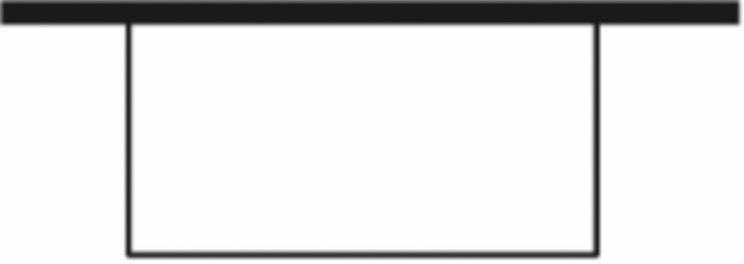
\includegraphics[width=0.28\textwidth]{figures/gao92_q8_fence.png}
\end{center}

\ifanswer
\solbegin
\step{设矩形的长为 $x$ 米，宽为 $y$，则 $xy=18$，}
\step{需要用栅栏长为 $x+2y\geqslant2\sqrt{2xy}=12$，}
\step{当且仅当 $x=2y$，即 $y=3$，$x=6$ 时取等号，故至少需要 $12$ 米栅栏.}
\solend
\fi

\item 已知 $a$ 为正整数，若关于 $x$ 的不等式 $\lvert x-2025\rvert\leqslant a$ 的解集中有且仅有 $7$ 个整数，则 $a$ 的值为\blankline[4.4em].

\ifanswer
\solbegin
\step{不等式 $\lvert x-2025\rvert\leqslant a$，则 $-a\leqslant x-2025\leqslant a$，即 $2025-a\leqslant x\leqslant2025+a$，}
\step{所以不等式 $\lvert x-2025\rvert\leqslant a$ 的解集为 $\{x\mid2025-a\leqslant x\leqslant2025+a\}$，}
\step{若不等式解集中有且仅有 $7$ 个整数，且 $a$ 为正整数，}
\step{由解集的对称性得这 $7$ 个整数以 $2025$ 为中心，向左右两边各延伸 $3$ 个整数，}
\step{即这 $7$ 个整数为 $2022,2023,2024,2025,2026,2027,2028$，所以 $a=3$.}
\solend
\fi

\item 已知关于 $x$ 的一元二次方程 $x^2-x+a=0$ 有两个不相等的正根 $m$、$n$，则 $\dfrac1m+\dfrac9n$ 的最小值为\blankline[4.4em].

\ifanswer
\solbegin
\step{因为一元二次方程 $x^2-x+a=0$ 有两个不相等的正根 $m$、$n$，}
\step{所以判别式 $\Delta=(-1)^2-4a>0\Rightarrow a<\dfrac14$，$m+n=1$，$mn=a>0$，}
\step{因此 $0<a<\dfrac14$ 且 $m+n=1(m,n>0)$.}
\step{$\dfrac1m+\dfrac9n=\left(\dfrac1m+\dfrac9n\right)(m+n)=1+\dfrac nm+\dfrac{9m}{n}+9=10+\dfrac nm+\dfrac{9m}{n}\geqslant10+2\sqrt9=16$，}
\step{等号成立条件为 $\dfrac nm=\dfrac{9m}{n}\Rightarrow n^2=9m^2\Rightarrow n=3m$，}
\step{$m$、$n>0$，结合 $m+n=1$，代入 $n=3m$ 得 $m+3m=1\Rightarrow m=\dfrac14$，$n=\dfrac34$，}
\step{此时 $mn=\dfrac14\cdot\dfrac34=\dfrac3{16}$，满足 $0<a<\dfrac14$，等号可取，因此 $\dfrac1m+\dfrac9n$ 的最小值为 $16$.}
\solend
\fi

\item 对任意 $A$、$B\subseteq R$，记 $A\oplus B=\{x\mid x\in A\cup B,x\notin A\cap B\}$，并称 $A\oplus B$ 为集合 $A$，$B$ 的对称差. 例如：若 $A=\{1,2,3\},B=\{2,3,4\}$，则 $A\oplus B=\{1,4\}$. 下列命题中，为真命题的有\blankline[4.4em].

①若 $A$、$B\subseteq R$ 且 $A\oplus B\subseteq A$，则 $A\subseteq B$

②若 $A$、$B\subseteq R$ 且 $A\oplus B=\varnothing$，则 $A=B$

③若 $A$、$B\subseteq R$ 且 $A\oplus B=B$，则 $A=\varnothing$

④对任意 $A$、$B\subseteq R$，都有 $A\oplus B=\complement_{R}A\oplus\complement_{R}B$

\ifanswer
\solbegin
\step{对于①，因为 $A\oplus B\subseteq A$，所以 $\{x\mid x\in A\cup B,x\notin A\cap B\}\subseteq A$，故 $B\subseteq A$，}
\step{故①错误；}
\step{对于②，$A$、$B\subseteq R$ 且 $A\oplus B=\varnothing$，则 $\varnothing=\{x\mid x\in A\cup B,x\notin A\cap B\}$，}
\step{即 $A\cup B=A\cap B$，所以 $A=B$，故②正确；}
\step{对于③，$A$、$B\subseteq R$ 且 $A\oplus B=B$，则 $B=\{x\mid x\in A\cup B,x\notin A\cap B\}$，}
\step{故 $A\subseteq B$，且 $B$ 中元素不在 $A\cap B$ 中，故 $A=\varnothing$，故③正确；}
\step{对于④，$\complement_{R}A\oplus\complement_{R}B=\{x\mid x\in\complement_{R}A\cup\complement_{R}B,x\notin\complement_{R}A\cap\complement_{R}B\}$，}
\step{其中 $\complement_{R}A\cup\complement_{R}B=\complement_{R}(A\cap B)$，$\complement_{R}A\cap\complement_{R}B=\complement_{R}(A\cup B)$，}
\step{故 $\complement_{R}A\oplus\complement_{R}B=\{x\mid x\in\complement_{R}(A\cap B)$，}
\step{$x\notin\complement_{R}(A\cup B)\}=\{x\mid x\in A\cup B,x\notin A\cap B\}$，}
\step{而 $A\oplus B=\{x\mid x\in A\cup B,x\notin A\cap B\}$，故 $A\oplus B=\complement_{R}A\oplus\complement_{R}B$，故④正确.}
\step{故正确的是②③④.}
\solend
\fi

\item 若不等式 $x^2-2ax+a^2-1\geqslant0$ 对任意 $x\in[0,2]$ 恒成立，则实数 $a$ 的取值范围是\blankline[4.4em].

\ifanswer
\solbegin
\step{由题意不等式 $x^2-2ax+a^2-1\geqslant0$ 对任意 $x\in[0,2]$ 恒成立，}
\step{解得 $x\leqslant a-1$ 或 $x\geqslant a+1$，要使此不等式对任意 $x\in[0,2]$ 恒成立，}
\step{则区间 $[0,2]$ 必须完全包含在解集 $(-\infty,a-1]\cup[a+1,+\infty)$ 中，}
\step{等价于 $[0,2]$ 与开区间 $(a-1,a+1)$ 的交集为空集，}
\step{区间 $[0,2]$ 在 $a-1$ 左侧，即 $2\leqslant a-1$，解得 $a\geqslant3$，}
\step{区间 $[0,2]$ 在 $a+1$ 右侧，即 $a+1\leqslant0$，解得 $a\leqslant-1$，}
\step{当 $a\in(-1,3)$，则 $(a-1,a+1)$ 与 $[0,2]$ 必有交集，不满足条件，}
\step{综上，实数 $a$ 的取值范围是 $(-\infty,-1]\cup[3,+\infty)$.}
\solend
\fi

\end{enumerate}

\bigsec{二、选择题}

\begin{enumerate}
\setcounter{enumi}{12}

\item 若 $a<b<0$，则下列不等式成立的是\mbox{（\quad）}% 原卷括号内已印“D”，试卷版按惯例留空

\keepwithprev
A. $a^2<b^2$\qquad B. $\dfrac1a<\dfrac1b$\qquad C. $ab<b^2$\qquad D. $ab<a^2$

\ifanswer
\ans{$D$}
\fi

\item 已知全集 $U=\{1,2,3,4,5\}$，集合 $A,B$ 是 $U$ 子集，满足 $\overline{A\cup B}=\{4,5\}$，$B=\{2,3\}$，则 $A\cap\overline B=\mbox{（\quad）}$

\keepwithprev
A. $\{1\}$\qquad B. $\{1,2\}$\qquad C. $\{1,4,5\}$\qquad D. $\varnothing$

\ifanswer
\solbegin
\step{因为全集 $U=\{1,2,3,4,5\}$，集合 $A$、$B$ 是 $U$ 子集，$\overline{A\cup B}=\{4,5\}$，$B=\{2,3\}$，}
\step{所以 $A\cup B=\{1,2,3\}$，故 $1\in A$，$1\notin B$，$4\notin A$，$5\notin A$，$4\notin B$，$5\notin B$，}
\step{故 $A\cap\overline B=\{1\}$. 故选 $A$.}
\solend
\fi

\item 设 $a>0$，若关于 $x$ 的不等式 $x^2-(2a-1)x-2a<0$ 的解集中恰有 $3$ 个整数，则实数 $a$ 的取值范围是\mbox{（\quad）}

\keepwithprev
A. $\left[1,\dfrac32\right]$\qquad B. $\left(1,\dfrac32\right]$\qquad C. $\left[\dfrac12,1\right]$\qquad D. $\left(\dfrac12,1\right]$

\ifanswer
\solbegin
\step{已知关于 $x$ 的不等式 $x^2-(2a-1)x-2a<0$，则 $(x+1)(x-2a)<0$，}
\step{则 $-1<x<2a$，又解集中恰有 $3$ 个整数，则 $2<2a\leqslant3$，则 $1<a\leqslant\dfrac32$，}
\step{则 $a$ 的取值范围为 $\left(1,\dfrac32\right]$. 故选 $B$.}
\solend
\fi

\item 已知集合 $U=\{1,2,3,\cdots,2027\}$，$M\subseteq U$，若对于 $M$ 中的任意两个不同的元素 $x$、$y$，都有 $\lvert x-y\rvert>2$，则 $M$ 中元素个数的最大值为\mbox{（\quad）}

\keepwithprev
A. $675$\qquad B. $676$\qquad C. $2025$\qquad D. $2026$

\ifanswer
\solbegin
\step{对于 $M$ 中的任意两个不同的元素 $x$、$y$，都有 $\lvert x-y\rvert>2$，}
\step{不妨设 $x>y$，都有 $x-y\geqslant3$，}
\step{要想 $M$ 所含元素个数最大，则要 $x-y$ 尽可能小，故需使得 $x-y$ 的最小值为 $3$，}
\step{将 $1\sim2027$ 这 $2027$ 个元素按如下分组：}
\step{$\{1,2,3\},\{4,5,6\},\cdots,\{2023,2024,2025\},\{2026,2027\}$，}
\step{故应在前 $675$ 组中按周期 $3$ 每组取一个元素，且第一组中不能取 $3$，}
\step{第一组中取 $1$ 时，得 $M=\{1,4,7,\cdots,2023,2026\}$}
\step{或 $M=\{1,4,7,\cdots,2023,2027\}$ 这样的集合，}
\step{第一组取 $2$ 时，得 $M=\{2,5,8,\cdots,2024,2027\}$，}
\step{其中任意两元素差值 $x-y(x>y)$ 都大于 $2$，满足题意，}
\step{故 $M$ 所含元素个数的最大值为 $\dfrac{2025}{3}+1=676$. 故选 $B$.}
\solend
\fi

\end{enumerate}

\bigsec{三、解答题}

\begin{enumerate}
\setcounter{enumi}{16}

\item 已知集合 $M=\{x\mid a-1\leqslant x\leqslant2a+3\}$，$P=\{x\mid-2<x\leqslant4\}$，全集 $U=R$.

（1）当 $a=2$ 时，求 $M\cap P$；

（2）若 $x\in P$ 是 $x\in M$ 的必要不充分条件，求实数 $a$ 的取值范围.

\ansspace*[9]

\ifanswer
\solbegin
\stepm{（1）}{当 $a=2$ 时，集合 $M=\{x\mid1\leqslant x\leqslant7\}$，所以 $M\cap P=\{x\mid1\leqslant x\leqslant4\}$；}
\stepm{（2）}{因为 $x\in P$ 是 $x\in M$ 的必要不充分条件，所以 $M\subsetneqq P$，}
\step{当 $M=\varnothing$ 时，$a-1>2a+3$，解得 $a<-4$，}
\step{当 $M\neq\varnothing$ 时，则 $\begin{cases}a-1\leqslant2a+3\\ a-1>-2\\ 2a+3\leqslant4\end{cases}$，解得 $-1<a\leqslant\dfrac12$，}
\step{综上所述，实数 $a$ 的取值范围为 $(-\infty,-4)\cup\left(-1,\dfrac12\right]$.}
\solend
\fi

\item 命题甲：关于 $x$ 的方程 $(a-1)x^2+(2a-4)x+a=0$ 有两个不相等的实数根；

命题乙：关于 $x$ 的不等式 $ax^2-2ax+a+1>0$ 的解集为 $R$.

（1）若命题甲为真命题，求实数 $a$ 的取值范围；

（2）若命题甲、乙中至多有一个为真命题，求实数 $a$ 的取值范围.

\ansspace*[12]

\ifanswer
\solbegin
\stepm{（1）}{命题甲：关于 $x$ 的方程 $(a-1)x^2+(2a-4)x+a=0$ 有两个不相等的实数根，}
\step{则 $\begin{cases}a-1\neq0\\ \Delta=(2a-4)^2-4a(a-1)>0\end{cases}$，解得 $a<\dfrac43$ 且 $a\neq1$，}
\step{故 $a$ 的范围为 $\left\{a\left|a<\dfrac43\ \text{且}\ a\neq1\right.\right\}$；}
\stepm{（2）}{当 $a=0$ 时 $y=1>0$，符合题意；}
\step{当 $a\neq0$，由 $\begin{cases}a>0\\ \Delta=4a^2-4a(a+1)<0\end{cases}$，解得 $a>0$，}
\step{则 $a$ 的取值范围为 $a\geqslant0$，}
\step{故 $p$、$q$ 都为真时，$a$ 的范围为 $0\leqslant a<\dfrac43$ 且 $a\neq1$，}
\step{则命题甲、乙中至多有一个为真命题时，}
\step{$a$ 的取值范围为 $\left\{a\left|a<0\ \text{或}\ a=1\ \text{或}\ a\geqslant\dfrac43\right.\right\}$.}
\solend
\fi

\item 如图，$OA$、$OB$ 是两条长度足够长的互相垂直的笔直小路，矩形 $OCPD$ 的顶点 $C$，$D$ 分别在 $OA$、$OB$ 上，且该矩形区域内种满了荷花. 为了让观赏者有更好的观赏体验，现计划经过点 $P$ 修一条小路 $EF$，其中点 $E$ 在小路 $OA$ 上，点 $F$ 在小路 $OB$ 上，并在 $\triangle OEF$ 区域内种满荷花. 已知 $OD=25$ m，$OC=40$ m，且小路 $EF$ 要完全位于一个以 $O$ 为顶点的，边长为 $100$ m 的正方形内部（包括边界）. 记 $\triangle OEF$ 的面积为 $S$ m$^2$.

\begin{center}
\begin{tikzpicture}[x=0.46cm,y=0.42cm,line width=0.7pt]
\draw (0,0) -- (0,10.2) node[above,inner sep=3pt] {$A$};
\draw (0,0) -- (11.8,0) node[right,inner sep=3pt] {$B$};
\draw (0,4.83) -- (2.42,4.83) -- (2.42,0);
\draw (0,6.92) -- (8.01,0);
\node[below left,inner sep=2pt] at (0,0) {$O$};
\node[below,inner sep=2pt] at (2.42,0) {$D$};
\node[left,inner sep=3pt] at (0,4.83) {$C$};
\node[above right,inner sep=1pt] at (2.42,4.83) {$P$};
\node[left,inner sep=3pt] at (0,6.92) {$E$};
\node[below,inner sep=2pt] at (8.01,0) {$F$};
\end{tikzpicture}
\end{center}

（1）设 $EC=x\cdot m$，试用 $x$ 表示 $OF$，并求 $x$ 的取值范围.

（2）当 $EC$ 的长度为多少时，$S$ 取得最小值？最小值是多少？

\ansspace*[11]

\ifanswer
\solbegin
\stepm{（1）}{由题意得 $x\leqslant60$，}
\step{$\triangle PCE\backsim\triangle FDP$，所以 $\dfrac{EC}{CP}=\dfrac{PD}{DF}$，即 $\dfrac{x}{25}=\dfrac{40}{DF}$，得 $DF=\dfrac{1000}{x}$ m，}
\step{所以 $OF=OD+DF=\left(25+\dfrac{1000}{x}\right)$ m，}
\step{所以 $25+\dfrac{1000}{x}\leqslant100$，解得 $x\geqslant\dfrac{40}{3}$；}
\step{综上，$\dfrac{40}{3}\leqslant x\leqslant60$；}
\stepm{（2）}{由 $OE=OC+CE=(40+x)$ m，}
\step{所以 $S=\dfrac12\cdot OF\cdot OE=\dfrac12\left(25+\dfrac{1000}{x}\right)(40+x)$}
\step{$=\dfrac12\left(1000+25x+\dfrac{40000}{x}+1000\right)$ m$^2$，}
\step{由基本不等式得 $S\geqslant\dfrac12\left(2000+2\sqrt{25x\cdot\dfrac{40000}{x}}\right)=2000$ m$^2$，}
\step{当且仅当 $25x=\dfrac{40000}{x}$，即 $x=40$ 时取等号，}
\step{故 $EC=40$ m 时，$S$ 取得最小值，为 $2000$ m$^2$.}
\solend
\fi

\item 已知函数 $f(x)=x^2-(a-2)x+a-3$.

（1）若 $f(x)=0$ 的两根为 $\alpha,\beta$，$\alpha^2+\beta^2=2$，求 $a$ 的值；

（2）解关于 $x$ 的不等式 $f(x)\geqslant0$；

（3）是否存在整数 $m,n$，使得关于 $x$ 的不等式 $m\leqslant f(x)\leqslant n$ 的解集恰好为 $[m,n]$？若存在，求出 $m,n$ 的值. 若不存在，请说明理由.

\ansspace*[16]

\ifanswer
\solbegin
\stepm{（1）}{由韦达定理，$\alpha+\beta=a-2,\alpha\beta=a-3$，}
\step{因此 $\alpha^2+\beta^2=(a-2)^2-2(a-3)=2\Leftrightarrow(a-2)(a-4)=0$，}
\step{$a=2$ 时两根为 $1,-1$；$a=4$ 时两根均为 $1$，均满足条件，}
\step{所以 $a=2$ 或 $a=4$.}
\stepm{（2）}{因为 $f(x)=(x-1)[x-(a-3)]$，所以分三种情况：}
\step{当 $a<4$ 时，$a-3<1$，解集为 $(-\infty,a-3]\cup[1,+\infty)$.}
\step{当 $a=4$ 时，$f(x)=(x-1)^2\geqslant0$ 恒成立，解集为 $R$.}
\step{当 $a>4$ 时，$a-3>1$，解集为 $(-\infty,1]\cup[a-3,+\infty)$.}
\stepm{（3）}{区间 $[m,n]$ 要求 $m<n$. 记 $f(x)$ 的最小值为 $k$.}
\step{$[m,n]$ 非空，不等式 $f(x)\leqslant n$ 有解，其解集为闭区间 $[x_1,x_2]$，}
\step{其中 $x_1\leqslant x_2$ 是方程 $f(x)=n$ 的两根.}
\step{若 $k<m$，则 $f(x)<m$ 的解集是 $[x_1,x_2]$ 内部的一个开区间，}
\step{从 $[x_1,x_2]$ 中去掉它后剩下两段，原不等式的解集不是一个区间，矛盾，}
\step{所以 $k\geqslant m$，原不等式的解集就是 $[x_1,x_2]$，于是 $m=x_1,n=x_2$，}
\step{即 $f(m)=f(n)=n$，于是 $f(m)-f(n)=(m-n)(m+n-a+2)=0$.}
\step{因为 $m\neq n$，所以 $a=m+n+2$.}
\step{代入 $f(m)=n$，得 $(m-1)(1-n)=n\Leftrightarrow m(n-1)=-1$，$m,n$ 均为整数，}
\step{因此 $(m,n)=(-1,2)$ 或 $(m,n)=(1,0)$.}
\step{结合 $m<n$，只可能有 $m=-1,n=2$，此时 $a=3$.}
\step{检验：此时 $f(x)=x^2-x$，且 $x^2-x=\left(x-\dfrac12\right)^2-\dfrac14\geqslant-\dfrac14>-1$，}
\step{因此 $-1\leqslant f(x)\leqslant2\Leftrightarrow x^2-x\leqslant2\Leftrightarrow(x+1)(x-2)\leqslant0\Leftrightarrow x\in[-1,2]$，}
\step{所以存在符合条件的整数 $m=-1,n=2$.}
\solend
\fi

\item 给定数集 $M$，若对于任意 $a$、$b\in M$，有 $a+b\in M,a-b\in M$，则称集合 $M$ 为闭集合.

（1）判断集合 $A_1=\{-4,-2,0,2,4\}$，集合 $B=\{x\mid x=3k,k\in\Z\}$ 是否为闭集合；

（2）若集合 $C$、$D$ 为闭集合，则 $C\cup D$ 是否一定为闭集合？请说明理由；

（3）已知集合 $C$、$D$ 为闭集合，且 $C\subsetneq R,D\subsetneq R$，证明：$(C\cup D)\subsetneq R$.% 原卷印作 (C∪D)⊂R，按解析证明的是 C∪D≠R，排真子集

\ansspace*[14]

\ifanswer
\solbegin
\stepm{（1）}{因为 $4\in A_1$，$2\in A_1$，$4+2=6\notin A_1$，所以 $A_1$ 不是闭集合；}
\step{任取 $x,y\in B$，设 $x=3m,y=3n,m,n\in\Z$，}
\step{则 $x+y=3m+3n=3(m+n)$ 且 $m+n\in\Z$，}
\step{所以 $x+y\in B$，同理，$x-y\in B$，故 $B$ 为闭集合.}
\stepm{（2）}{结论：不一定.}
\step{不妨令 $C=\{x\mid x=2k,k\in\Z\},D=\{x\mid x=3k,k\in\Z\}$，}
\step{则由（1）得 $C$、$D$ 为闭集合，易得 $2,3\in C\cup D,2+3=5\notin C\cup D$，}
\step{因此，$C\cup D$ 不一定是闭集合.}
\stepm{（3）}{不妨假设 $C\cup D=R$，则由 $C\subsetneq R$，得存在 $a\in R$ 且 $a\notin C$，故 $a\in D$.}
\step{同理，存在 $b\in R$ 且 $b\notin D$，故 $b\in C$.}
\step{因为 $a+b\in R=C\cup D$，所以 $a+b\in C$ 或 $a+b\in D$.}
\step{若 $a+b\in C$，则由 $C$ 为闭集合且 $b\in C$，得 $a=(a+b)-b\in C$，}
\step{与 $a\notin C$ 矛盾.}
\step{若 $a+b\in D$，则由 $D$ 为闭集合且 $a\in D$，得 $b=(a+b)-a\in D$，}
\step{与 $b\notin D$ 矛盾.}
\step{综上，$C\cup D=R$ 不成立，故 $(C\cup D)\subsetneq R$.}
\solend
\fi

\end{enumerate}

\end{document}
"
% 紧凑版：xelatex "\def\iscompact{1}% 高一92_闵行实验_10月月考.tex
%   —— 高一上数学“2026-2027 年闵行实验高一上 10 月月考”（讲评版）
% 试卷版：xelatex 高一92_闵行实验_10月月考.tex
% 答案版：xelatex "\def\isanswer{1}\input{高一92_闵行实验_10月月考.tex}"
% 紧凑版：xelatex "\def\iscompact{1}\input{高一92_闵行实验_10月月考.tex}"
%
% 原始材料：微信公众号“魔都数学加油站”文章，连载“27学年高一92”；
% 原文标题“27学年高一92——2026-2027年上海市闵行实验高一上10月月考”；
% 原文链接：https://mp.weixin.qq.com/s/8HUyr3G7GpcHyczwu_XYCQ。
% 正文为 10 张 PNG 页（`原图/高一92_闵行实验_10月月考/01..10.png`），均 4762×6735，按页序读取。
%
% 篇幅与题号：原卷自第 3 题起编号（第 1、2 题不在原文内）。填空题 3—12（10 题）、
% 选择题 13—16（4 题）、解答题 17—21（5 题），共 19 题。
%
% 讲评版：第 6 题只印【答案】（“$[-1,3]$”），本稿只给 \ans{}；第 13 题无【解析】、
% 答案“D”直接印在题干括号内，本稿试卷版按惯例留空、答案版提 \ans{$D$}；其余 17 题印
% 【解析】，其中选择题答案在解析末句“故选 $A$／$B$／$B$”。
% 第 8 题题干右侧有一幅“围墙 + 三面栅栏”示意图（裁自第 2 页原图）；第 19 题题干带
% 与 高一88 第 19 题同型的示意图（$OA$／$OB$ 两条小路、矩形 $OCPD$、折线 $EF$），用 TikZ 重绘。
%
% 副标题：原卷未印副标题。本稿按内容标作“集合与常用逻辑用语、不等式”。
%
% 原卷笔误/存疑（均照录未改，正文对应处另有 % 注）：
%   ① 第 21 题 (3) 题干与解析末句把结论印作“$(C\cup D)\subset R$”，而解析证明的是
%      “$C\cup D=\R$ 不成立”，按文意应为“$(C\cup D)\subsetneq\R$”；本稿按真子集排
%      $\subsetneq$，原卷记号照录于文件头；
%   ② 第 7 题解析只列 $B=\varnothing$（$a=0$）、$B=\{1\}$（$a=1$）、$B=\{-3\}$（$a=-\frac13$）
%      三种情形，与结论 $\left\{0,1,-\frac13\right\}$ 相符，无笔误。
%
% 与原卷的排版差异：
%   ① 原卷每题下直接印【答案】/【解析】，本稿按全稿惯例将答案与解析置于答案版；
%   ② 原卷未印副标题，本稿补出；填空横线统一排 \blankline[4.4em]；
%   ③ 原卷数集记号排斜体 $R$、$Z$，本稿按全稿惯例改用 $\R$、$\Z$；
%   ④ 第 17—21 题的子问用行内“（1）（2）（3）”段，解析中的子问标号用 \stepm；
%   ⑤ 解答题按惯例加 \ansspace；选择题括号排 \mbox{（\quad）}；
%   ⑥ 第 8 题的示意图原卷排在题干右侧、文字绕排，本稿改排为题干后的居中图
%      （自原图裁切、去粉色水印后转灰度）；第 19 题的图按原图比例 TikZ 重绘。
%
% 行数核对：逐题数 \step/\stepm 条数，合计 128 条（Q3：2；Q4：3；Q5：2；Q6：0；Q7：6；
% Q8：3；Q9：5；Q10：7；Q11：12；Q12：8；Q13：0；Q14：3；Q15：3；Q16：11；Q17：5；
% Q18：9；Q19：11；Q20：22；Q21：16）。第 6 题只印答案、第 13 题无解析，均不计入 \step 账。
% 原卷解析的换行按语意合并，未逐行强拆。
%
\documentclass[a4paper,11pt]{article}
\usepackage{common}

\begin{document}

\examtitlest[7]{2026--2027 年闵行实验高一上 10 月月考}{集合与常用逻辑用语、不等式}

\bigsec{一、填空题}

\begin{enumerate}
\setcounter{enumi}{2}

\item 已知 $3<a<8$，$4<b<9$，则 $\dfrac ab$ 的取值范围是\blankline[4.4em].

\ifanswer
\solbegin
\step{因为 $4<b<9$，所以 $\dfrac19<\dfrac1b<\dfrac14$，又 $3<a<8$，所以 $\dfrac13<\dfrac ab<2$，}
\step{故 $\dfrac ab$ 的取值范围是 $\left(\dfrac13,2\right)$.}
\solend
\fi

\item 已知 $p:x>3$，$q:x>5$，则 $p$ 是 $q$ 的\blankline[4.4em]（选“充分不必要条件”“必要不充分条件”“充要条件”“既不充分也不必要条件”之一填空）.

\ifanswer
\solbegin
\step{当 $x>3$ 时，不能推出 $x>5$，充分性不成立；}
\step{当 $x>5$ 时，可以得到 $x>3$，必要性成立；}
\step{故 $p$ 是 $q$ 的必要不充分条件.}
\solend
\fi

\item 不等式 $\dfrac{x-1}{2x+1}\leqslant1$ 的解集为\blankline[4.4em].

\ifanswer
\solbegin
\step{因为 $\dfrac{x-1}{2x+1}\leqslant1$，所以 $\dfrac{x-1}{2x+1}-\dfrac{2x+1}{2x+1}\leqslant0$，所以 $\dfrac{x+2}{2x+1}\geqslant0$，}
\step{所以 $x>-\dfrac12$ 或 $x\leqslant-2$，即不等式的解集是 $(-\infty,-2]\cup\left(-\dfrac12,+\infty\right)$.}
\solend
\fi

\item 设 $x\in R$，则方程 $\lvert x+1\rvert+\lvert x-3\rvert=4$ 的解集为\blankline[4.4em].

\ifanswer
\ans{$[-1,3]$}
\fi

\item 若 $A=\{x\mid x^2+2x=3\}$，$B=\{x\mid ax=1\}$，且 $B\subseteq A$，则实数 $a$ 的值组成的集合为\blankline[4.4em].

\ifanswer
\solbegin
\step{由 $x^2+2x=3$ 得 $x^2+2x-3=0$，解得 $x=1$ 或 $x=-3$，所以 $A=\{1,-3\}$，}
\step{又因为 $B=\{x\mid ax=1\}$，且 $B\subseteq A$，}
\step{当 $B=\varnothing$，即 $a=0$ 时，显然符合题意；}
\step{当 $B=\{1\}$，即 $a=1$ 时，也符合题意；}
\step{当 $B=\{-3\}$，即 $a=-\dfrac13$ 时，也符合题意；}
\step{综上所述，实数 $a$ 的值组成的集合为 $\left\{0,1,-\dfrac13\right\}$.}
\solend
\fi

\item 某校欲在围墙边用栅栏围成一个 $18$ 平方米的矩形区域，作为天鹅的地面栖息地，矩形区域的一条边为围墙（如图），则至少需要\blankline[4.4em]米栅栏.

\begin{center}
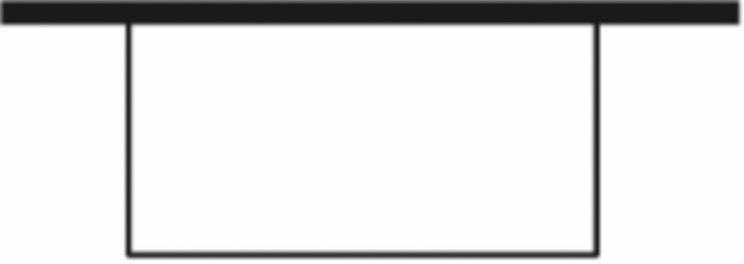
\includegraphics[width=0.28\textwidth]{figures/gao92_q8_fence.png}
\end{center}

\ifanswer
\solbegin
\step{设矩形的长为 $x$ 米，宽为 $y$，则 $xy=18$，}
\step{需要用栅栏长为 $x+2y\geqslant2\sqrt{2xy}=12$，}
\step{当且仅当 $x=2y$，即 $y=3$，$x=6$ 时取等号，故至少需要 $12$ 米栅栏.}
\solend
\fi

\item 已知 $a$ 为正整数，若关于 $x$ 的不等式 $\lvert x-2025\rvert\leqslant a$ 的解集中有且仅有 $7$ 个整数，则 $a$ 的值为\blankline[4.4em].

\ifanswer
\solbegin
\step{不等式 $\lvert x-2025\rvert\leqslant a$，则 $-a\leqslant x-2025\leqslant a$，即 $2025-a\leqslant x\leqslant2025+a$，}
\step{所以不等式 $\lvert x-2025\rvert\leqslant a$ 的解集为 $\{x\mid2025-a\leqslant x\leqslant2025+a\}$，}
\step{若不等式解集中有且仅有 $7$ 个整数，且 $a$ 为正整数，}
\step{由解集的对称性得这 $7$ 个整数以 $2025$ 为中心，向左右两边各延伸 $3$ 个整数，}
\step{即这 $7$ 个整数为 $2022,2023,2024,2025,2026,2027,2028$，所以 $a=3$.}
\solend
\fi

\item 已知关于 $x$ 的一元二次方程 $x^2-x+a=0$ 有两个不相等的正根 $m$、$n$，则 $\dfrac1m+\dfrac9n$ 的最小值为\blankline[4.4em].

\ifanswer
\solbegin
\step{因为一元二次方程 $x^2-x+a=0$ 有两个不相等的正根 $m$、$n$，}
\step{所以判别式 $\Delta=(-1)^2-4a>0\Rightarrow a<\dfrac14$，$m+n=1$，$mn=a>0$，}
\step{因此 $0<a<\dfrac14$ 且 $m+n=1(m,n>0)$.}
\step{$\dfrac1m+\dfrac9n=\left(\dfrac1m+\dfrac9n\right)(m+n)=1+\dfrac nm+\dfrac{9m}{n}+9=10+\dfrac nm+\dfrac{9m}{n}\geqslant10+2\sqrt9=16$，}
\step{等号成立条件为 $\dfrac nm=\dfrac{9m}{n}\Rightarrow n^2=9m^2\Rightarrow n=3m$，}
\step{$m$、$n>0$，结合 $m+n=1$，代入 $n=3m$ 得 $m+3m=1\Rightarrow m=\dfrac14$，$n=\dfrac34$，}
\step{此时 $mn=\dfrac14\cdot\dfrac34=\dfrac3{16}$，满足 $0<a<\dfrac14$，等号可取，因此 $\dfrac1m+\dfrac9n$ 的最小值为 $16$.}
\solend
\fi

\item 对任意 $A$、$B\subseteq R$，记 $A\oplus B=\{x\mid x\in A\cup B,x\notin A\cap B\}$，并称 $A\oplus B$ 为集合 $A$，$B$ 的对称差. 例如：若 $A=\{1,2,3\},B=\{2,3,4\}$，则 $A\oplus B=\{1,4\}$. 下列命题中，为真命题的有\blankline[4.4em].

①若 $A$、$B\subseteq R$ 且 $A\oplus B\subseteq A$，则 $A\subseteq B$

②若 $A$、$B\subseteq R$ 且 $A\oplus B=\varnothing$，则 $A=B$

③若 $A$、$B\subseteq R$ 且 $A\oplus B=B$，则 $A=\varnothing$

④对任意 $A$、$B\subseteq R$，都有 $A\oplus B=\complement_{R}A\oplus\complement_{R}B$

\ifanswer
\solbegin
\step{对于①，因为 $A\oplus B\subseteq A$，所以 $\{x\mid x\in A\cup B,x\notin A\cap B\}\subseteq A$，故 $B\subseteq A$，}
\step{故①错误；}
\step{对于②，$A$、$B\subseteq R$ 且 $A\oplus B=\varnothing$，则 $\varnothing=\{x\mid x\in A\cup B,x\notin A\cap B\}$，}
\step{即 $A\cup B=A\cap B$，所以 $A=B$，故②正确；}
\step{对于③，$A$、$B\subseteq R$ 且 $A\oplus B=B$，则 $B=\{x\mid x\in A\cup B,x\notin A\cap B\}$，}
\step{故 $A\subseteq B$，且 $B$ 中元素不在 $A\cap B$ 中，故 $A=\varnothing$，故③正确；}
\step{对于④，$\complement_{R}A\oplus\complement_{R}B=\{x\mid x\in\complement_{R}A\cup\complement_{R}B,x\notin\complement_{R}A\cap\complement_{R}B\}$，}
\step{其中 $\complement_{R}A\cup\complement_{R}B=\complement_{R}(A\cap B)$，$\complement_{R}A\cap\complement_{R}B=\complement_{R}(A\cup B)$，}
\step{故 $\complement_{R}A\oplus\complement_{R}B=\{x\mid x\in\complement_{R}(A\cap B)$，}
\step{$x\notin\complement_{R}(A\cup B)\}=\{x\mid x\in A\cup B,x\notin A\cap B\}$，}
\step{而 $A\oplus B=\{x\mid x\in A\cup B,x\notin A\cap B\}$，故 $A\oplus B=\complement_{R}A\oplus\complement_{R}B$，故④正确.}
\step{故正确的是②③④.}
\solend
\fi

\item 若不等式 $x^2-2ax+a^2-1\geqslant0$ 对任意 $x\in[0,2]$ 恒成立，则实数 $a$ 的取值范围是\blankline[4.4em].

\ifanswer
\solbegin
\step{由题意不等式 $x^2-2ax+a^2-1\geqslant0$ 对任意 $x\in[0,2]$ 恒成立，}
\step{解得 $x\leqslant a-1$ 或 $x\geqslant a+1$，要使此不等式对任意 $x\in[0,2]$ 恒成立，}
\step{则区间 $[0,2]$ 必须完全包含在解集 $(-\infty,a-1]\cup[a+1,+\infty)$ 中，}
\step{等价于 $[0,2]$ 与开区间 $(a-1,a+1)$ 的交集为空集，}
\step{区间 $[0,2]$ 在 $a-1$ 左侧，即 $2\leqslant a-1$，解得 $a\geqslant3$，}
\step{区间 $[0,2]$ 在 $a+1$ 右侧，即 $a+1\leqslant0$，解得 $a\leqslant-1$，}
\step{当 $a\in(-1,3)$，则 $(a-1,a+1)$ 与 $[0,2]$ 必有交集，不满足条件，}
\step{综上，实数 $a$ 的取值范围是 $(-\infty,-1]\cup[3,+\infty)$.}
\solend
\fi

\end{enumerate}

\bigsec{二、选择题}

\begin{enumerate}
\setcounter{enumi}{12}

\item 若 $a<b<0$，则下列不等式成立的是\mbox{（\quad）}% 原卷括号内已印“D”，试卷版按惯例留空

\keepwithprev
A. $a^2<b^2$\qquad B. $\dfrac1a<\dfrac1b$\qquad C. $ab<b^2$\qquad D. $ab<a^2$

\ifanswer
\ans{$D$}
\fi

\item 已知全集 $U=\{1,2,3,4,5\}$，集合 $A,B$ 是 $U$ 子集，满足 $\overline{A\cup B}=\{4,5\}$，$B=\{2,3\}$，则 $A\cap\overline B=\mbox{（\quad）}$

\keepwithprev
A. $\{1\}$\qquad B. $\{1,2\}$\qquad C. $\{1,4,5\}$\qquad D. $\varnothing$

\ifanswer
\solbegin
\step{因为全集 $U=\{1,2,3,4,5\}$，集合 $A$、$B$ 是 $U$ 子集，$\overline{A\cup B}=\{4,5\}$，$B=\{2,3\}$，}
\step{所以 $A\cup B=\{1,2,3\}$，故 $1\in A$，$1\notin B$，$4\notin A$，$5\notin A$，$4\notin B$，$5\notin B$，}
\step{故 $A\cap\overline B=\{1\}$. 故选 $A$.}
\solend
\fi

\item 设 $a>0$，若关于 $x$ 的不等式 $x^2-(2a-1)x-2a<0$ 的解集中恰有 $3$ 个整数，则实数 $a$ 的取值范围是\mbox{（\quad）}

\keepwithprev
A. $\left[1,\dfrac32\right]$\qquad B. $\left(1,\dfrac32\right]$\qquad C. $\left[\dfrac12,1\right]$\qquad D. $\left(\dfrac12,1\right]$

\ifanswer
\solbegin
\step{已知关于 $x$ 的不等式 $x^2-(2a-1)x-2a<0$，则 $(x+1)(x-2a)<0$，}
\step{则 $-1<x<2a$，又解集中恰有 $3$ 个整数，则 $2<2a\leqslant3$，则 $1<a\leqslant\dfrac32$，}
\step{则 $a$ 的取值范围为 $\left(1,\dfrac32\right]$. 故选 $B$.}
\solend
\fi

\item 已知集合 $U=\{1,2,3,\cdots,2027\}$，$M\subseteq U$，若对于 $M$ 中的任意两个不同的元素 $x$、$y$，都有 $\lvert x-y\rvert>2$，则 $M$ 中元素个数的最大值为\mbox{（\quad）}

\keepwithprev
A. $675$\qquad B. $676$\qquad C. $2025$\qquad D. $2026$

\ifanswer
\solbegin
\step{对于 $M$ 中的任意两个不同的元素 $x$、$y$，都有 $\lvert x-y\rvert>2$，}
\step{不妨设 $x>y$，都有 $x-y\geqslant3$，}
\step{要想 $M$ 所含元素个数最大，则要 $x-y$ 尽可能小，故需使得 $x-y$ 的最小值为 $3$，}
\step{将 $1\sim2027$ 这 $2027$ 个元素按如下分组：}
\step{$\{1,2,3\},\{4,5,6\},\cdots,\{2023,2024,2025\},\{2026,2027\}$，}
\step{故应在前 $675$ 组中按周期 $3$ 每组取一个元素，且第一组中不能取 $3$，}
\step{第一组中取 $1$ 时，得 $M=\{1,4,7,\cdots,2023,2026\}$}
\step{或 $M=\{1,4,7,\cdots,2023,2027\}$ 这样的集合，}
\step{第一组取 $2$ 时，得 $M=\{2,5,8,\cdots,2024,2027\}$，}
\step{其中任意两元素差值 $x-y(x>y)$ 都大于 $2$，满足题意，}
\step{故 $M$ 所含元素个数的最大值为 $\dfrac{2025}{3}+1=676$. 故选 $B$.}
\solend
\fi

\end{enumerate}

\bigsec{三、解答题}

\begin{enumerate}
\setcounter{enumi}{16}

\item 已知集合 $M=\{x\mid a-1\leqslant x\leqslant2a+3\}$，$P=\{x\mid-2<x\leqslant4\}$，全集 $U=R$.

（1）当 $a=2$ 时，求 $M\cap P$；

（2）若 $x\in P$ 是 $x\in M$ 的必要不充分条件，求实数 $a$ 的取值范围.

\ansspace*[9]

\ifanswer
\solbegin
\stepm{（1）}{当 $a=2$ 时，集合 $M=\{x\mid1\leqslant x\leqslant7\}$，所以 $M\cap P=\{x\mid1\leqslant x\leqslant4\}$；}
\stepm{（2）}{因为 $x\in P$ 是 $x\in M$ 的必要不充分条件，所以 $M\subsetneqq P$，}
\step{当 $M=\varnothing$ 时，$a-1>2a+3$，解得 $a<-4$，}
\step{当 $M\neq\varnothing$ 时，则 $\begin{cases}a-1\leqslant2a+3\\ a-1>-2\\ 2a+3\leqslant4\end{cases}$，解得 $-1<a\leqslant\dfrac12$，}
\step{综上所述，实数 $a$ 的取值范围为 $(-\infty,-4)\cup\left(-1,\dfrac12\right]$.}
\solend
\fi

\item 命题甲：关于 $x$ 的方程 $(a-1)x^2+(2a-4)x+a=0$ 有两个不相等的实数根；

命题乙：关于 $x$ 的不等式 $ax^2-2ax+a+1>0$ 的解集为 $R$.

（1）若命题甲为真命题，求实数 $a$ 的取值范围；

（2）若命题甲、乙中至多有一个为真命题，求实数 $a$ 的取值范围.

\ansspace*[12]

\ifanswer
\solbegin
\stepm{（1）}{命题甲：关于 $x$ 的方程 $(a-1)x^2+(2a-4)x+a=0$ 有两个不相等的实数根，}
\step{则 $\begin{cases}a-1\neq0\\ \Delta=(2a-4)^2-4a(a-1)>0\end{cases}$，解得 $a<\dfrac43$ 且 $a\neq1$，}
\step{故 $a$ 的范围为 $\left\{a\left|a<\dfrac43\ \text{且}\ a\neq1\right.\right\}$；}
\stepm{（2）}{当 $a=0$ 时 $y=1>0$，符合题意；}
\step{当 $a\neq0$，由 $\begin{cases}a>0\\ \Delta=4a^2-4a(a+1)<0\end{cases}$，解得 $a>0$，}
\step{则 $a$ 的取值范围为 $a\geqslant0$，}
\step{故 $p$、$q$ 都为真时，$a$ 的范围为 $0\leqslant a<\dfrac43$ 且 $a\neq1$，}
\step{则命题甲、乙中至多有一个为真命题时，}
\step{$a$ 的取值范围为 $\left\{a\left|a<0\ \text{或}\ a=1\ \text{或}\ a\geqslant\dfrac43\right.\right\}$.}
\solend
\fi

\item 如图，$OA$、$OB$ 是两条长度足够长的互相垂直的笔直小路，矩形 $OCPD$ 的顶点 $C$，$D$ 分别在 $OA$、$OB$ 上，且该矩形区域内种满了荷花. 为了让观赏者有更好的观赏体验，现计划经过点 $P$ 修一条小路 $EF$，其中点 $E$ 在小路 $OA$ 上，点 $F$ 在小路 $OB$ 上，并在 $\triangle OEF$ 区域内种满荷花. 已知 $OD=25$ m，$OC=40$ m，且小路 $EF$ 要完全位于一个以 $O$ 为顶点的，边长为 $100$ m 的正方形内部（包括边界）. 记 $\triangle OEF$ 的面积为 $S$ m$^2$.

\begin{center}
\begin{tikzpicture}[x=0.46cm,y=0.42cm,line width=0.7pt]
\draw (0,0) -- (0,10.2) node[above,inner sep=3pt] {$A$};
\draw (0,0) -- (11.8,0) node[right,inner sep=3pt] {$B$};
\draw (0,4.83) -- (2.42,4.83) -- (2.42,0);
\draw (0,6.92) -- (8.01,0);
\node[below left,inner sep=2pt] at (0,0) {$O$};
\node[below,inner sep=2pt] at (2.42,0) {$D$};
\node[left,inner sep=3pt] at (0,4.83) {$C$};
\node[above right,inner sep=1pt] at (2.42,4.83) {$P$};
\node[left,inner sep=3pt] at (0,6.92) {$E$};
\node[below,inner sep=2pt] at (8.01,0) {$F$};
\end{tikzpicture}
\end{center}

（1）设 $EC=x\cdot m$，试用 $x$ 表示 $OF$，并求 $x$ 的取值范围.

（2）当 $EC$ 的长度为多少时，$S$ 取得最小值？最小值是多少？

\ansspace*[11]

\ifanswer
\solbegin
\stepm{（1）}{由题意得 $x\leqslant60$，}
\step{$\triangle PCE\backsim\triangle FDP$，所以 $\dfrac{EC}{CP}=\dfrac{PD}{DF}$，即 $\dfrac{x}{25}=\dfrac{40}{DF}$，得 $DF=\dfrac{1000}{x}$ m，}
\step{所以 $OF=OD+DF=\left(25+\dfrac{1000}{x}\right)$ m，}
\step{所以 $25+\dfrac{1000}{x}\leqslant100$，解得 $x\geqslant\dfrac{40}{3}$；}
\step{综上，$\dfrac{40}{3}\leqslant x\leqslant60$；}
\stepm{（2）}{由 $OE=OC+CE=(40+x)$ m，}
\step{所以 $S=\dfrac12\cdot OF\cdot OE=\dfrac12\left(25+\dfrac{1000}{x}\right)(40+x)$}
\step{$=\dfrac12\left(1000+25x+\dfrac{40000}{x}+1000\right)$ m$^2$，}
\step{由基本不等式得 $S\geqslant\dfrac12\left(2000+2\sqrt{25x\cdot\dfrac{40000}{x}}\right)=2000$ m$^2$，}
\step{当且仅当 $25x=\dfrac{40000}{x}$，即 $x=40$ 时取等号，}
\step{故 $EC=40$ m 时，$S$ 取得最小值，为 $2000$ m$^2$.}
\solend
\fi

\item 已知函数 $f(x)=x^2-(a-2)x+a-3$.

（1）若 $f(x)=0$ 的两根为 $\alpha,\beta$，$\alpha^2+\beta^2=2$，求 $a$ 的值；

（2）解关于 $x$ 的不等式 $f(x)\geqslant0$；

（3）是否存在整数 $m,n$，使得关于 $x$ 的不等式 $m\leqslant f(x)\leqslant n$ 的解集恰好为 $[m,n]$？若存在，求出 $m,n$ 的值. 若不存在，请说明理由.

\ansspace*[16]

\ifanswer
\solbegin
\stepm{（1）}{由韦达定理，$\alpha+\beta=a-2,\alpha\beta=a-3$，}
\step{因此 $\alpha^2+\beta^2=(a-2)^2-2(a-3)=2\Leftrightarrow(a-2)(a-4)=0$，}
\step{$a=2$ 时两根为 $1,-1$；$a=4$ 时两根均为 $1$，均满足条件，}
\step{所以 $a=2$ 或 $a=4$.}
\stepm{（2）}{因为 $f(x)=(x-1)[x-(a-3)]$，所以分三种情况：}
\step{当 $a<4$ 时，$a-3<1$，解集为 $(-\infty,a-3]\cup[1,+\infty)$.}
\step{当 $a=4$ 时，$f(x)=(x-1)^2\geqslant0$ 恒成立，解集为 $R$.}
\step{当 $a>4$ 时，$a-3>1$，解集为 $(-\infty,1]\cup[a-3,+\infty)$.}
\stepm{（3）}{区间 $[m,n]$ 要求 $m<n$. 记 $f(x)$ 的最小值为 $k$.}
\step{$[m,n]$ 非空，不等式 $f(x)\leqslant n$ 有解，其解集为闭区间 $[x_1,x_2]$，}
\step{其中 $x_1\leqslant x_2$ 是方程 $f(x)=n$ 的两根.}
\step{若 $k<m$，则 $f(x)<m$ 的解集是 $[x_1,x_2]$ 内部的一个开区间，}
\step{从 $[x_1,x_2]$ 中去掉它后剩下两段，原不等式的解集不是一个区间，矛盾，}
\step{所以 $k\geqslant m$，原不等式的解集就是 $[x_1,x_2]$，于是 $m=x_1,n=x_2$，}
\step{即 $f(m)=f(n)=n$，于是 $f(m)-f(n)=(m-n)(m+n-a+2)=0$.}
\step{因为 $m\neq n$，所以 $a=m+n+2$.}
\step{代入 $f(m)=n$，得 $(m-1)(1-n)=n\Leftrightarrow m(n-1)=-1$，$m,n$ 均为整数，}
\step{因此 $(m,n)=(-1,2)$ 或 $(m,n)=(1,0)$.}
\step{结合 $m<n$，只可能有 $m=-1,n=2$，此时 $a=3$.}
\step{检验：此时 $f(x)=x^2-x$，且 $x^2-x=\left(x-\dfrac12\right)^2-\dfrac14\geqslant-\dfrac14>-1$，}
\step{因此 $-1\leqslant f(x)\leqslant2\Leftrightarrow x^2-x\leqslant2\Leftrightarrow(x+1)(x-2)\leqslant0\Leftrightarrow x\in[-1,2]$，}
\step{所以存在符合条件的整数 $m=-1,n=2$.}
\solend
\fi

\item 给定数集 $M$，若对于任意 $a$、$b\in M$，有 $a+b\in M,a-b\in M$，则称集合 $M$ 为闭集合.

（1）判断集合 $A_1=\{-4,-2,0,2,4\}$，集合 $B=\{x\mid x=3k,k\in\Z\}$ 是否为闭集合；

（2）若集合 $C$、$D$ 为闭集合，则 $C\cup D$ 是否一定为闭集合？请说明理由；

（3）已知集合 $C$、$D$ 为闭集合，且 $C\subsetneq R,D\subsetneq R$，证明：$(C\cup D)\subsetneq R$.% 原卷印作 (C∪D)⊂R，按解析证明的是 C∪D≠R，排真子集

\ansspace*[14]

\ifanswer
\solbegin
\stepm{（1）}{因为 $4\in A_1$，$2\in A_1$，$4+2=6\notin A_1$，所以 $A_1$ 不是闭集合；}
\step{任取 $x,y\in B$，设 $x=3m,y=3n,m,n\in\Z$，}
\step{则 $x+y=3m+3n=3(m+n)$ 且 $m+n\in\Z$，}
\step{所以 $x+y\in B$，同理，$x-y\in B$，故 $B$ 为闭集合.}
\stepm{（2）}{结论：不一定.}
\step{不妨令 $C=\{x\mid x=2k,k\in\Z\},D=\{x\mid x=3k,k\in\Z\}$，}
\step{则由（1）得 $C$、$D$ 为闭集合，易得 $2,3\in C\cup D,2+3=5\notin C\cup D$，}
\step{因此，$C\cup D$ 不一定是闭集合.}
\stepm{（3）}{不妨假设 $C\cup D=R$，则由 $C\subsetneq R$，得存在 $a\in R$ 且 $a\notin C$，故 $a\in D$.}
\step{同理，存在 $b\in R$ 且 $b\notin D$，故 $b\in C$.}
\step{因为 $a+b\in R=C\cup D$，所以 $a+b\in C$ 或 $a+b\in D$.}
\step{若 $a+b\in C$，则由 $C$ 为闭集合且 $b\in C$，得 $a=(a+b)-b\in C$，}
\step{与 $a\notin C$ 矛盾.}
\step{若 $a+b\in D$，则由 $D$ 为闭集合且 $a\in D$，得 $b=(a+b)-a\in D$，}
\step{与 $b\notin D$ 矛盾.}
\step{综上，$C\cup D=R$ 不成立，故 $(C\cup D)\subsetneq R$.}
\solend
\fi

\end{enumerate}

\end{document}
"
%
% 原始材料：微信公众号“魔都数学加油站”文章，连载“27学年高一92”；
% 原文标题“27学年高一92——2026-2027年上海市闵行实验高一上10月月考”；
% 原文链接：https://mp.weixin.qq.com/s/8HUyr3G7GpcHyczwu_XYCQ。
% 正文为 10 张 PNG 页（`原图/高一92_闵行实验_10月月考/01..10.png`），均 4762×6735，按页序读取。
%
% 篇幅与题号：原卷自第 3 题起编号（第 1、2 题不在原文内）。填空题 3—12（10 题）、
% 选择题 13—16（4 题）、解答题 17—21（5 题），共 19 题。
%
% 讲评版：第 6 题只印【答案】（“$[-1,3]$”），本稿只给 \ans{}；第 13 题无【解析】、
% 答案“D”直接印在题干括号内，本稿试卷版按惯例留空、答案版提 \ans{$D$}；其余 17 题印
% 【解析】，其中选择题答案在解析末句“故选 $A$／$B$／$B$”。
% 第 8 题题干右侧有一幅“围墙 + 三面栅栏”示意图（裁自第 2 页原图）；第 19 题题干带
% 与 高一88 第 19 题同型的示意图（$OA$／$OB$ 两条小路、矩形 $OCPD$、折线 $EF$），用 TikZ 重绘。
%
% 副标题：原卷未印副标题。本稿按内容标作“集合与常用逻辑用语、不等式”。
%
% 原卷笔误/存疑（均照录未改，正文对应处另有 % 注）：
%   ① 第 21 题 (3) 题干与解析末句把结论印作“$(C\cup D)\subset R$”，而解析证明的是
%      “$C\cup D=\R$ 不成立”，按文意应为“$(C\cup D)\subsetneq\R$”；本稿按真子集排
%      $\subsetneq$，原卷记号照录于文件头；
%   ② 第 7 题解析只列 $B=\varnothing$（$a=0$）、$B=\{1\}$（$a=1$）、$B=\{-3\}$（$a=-\frac13$）
%      三种情形，与结论 $\left\{0,1,-\frac13\right\}$ 相符，无笔误。
%
% 与原卷的排版差异：
%   ① 原卷每题下直接印【答案】/【解析】，本稿按全稿惯例将答案与解析置于答案版；
%   ② 原卷未印副标题，本稿补出；填空横线统一排 \blankline[4.4em]；
%   ③ 原卷数集记号排斜体 $R$、$Z$，本稿按全稿惯例改用 $\R$、$\Z$；
%   ④ 第 17—21 题的子问用行内“（1）（2）（3）”段，解析中的子问标号用 \stepm；
%   ⑤ 解答题按惯例加 \ansspace；选择题括号排 \mbox{（\quad）}；
%   ⑥ 第 8 题的示意图原卷排在题干右侧、文字绕排，本稿改排为题干后的居中图
%      （自原图裁切、去粉色水印后转灰度）；第 19 题的图按原图比例 TikZ 重绘。
%
% 行数核对：逐题数 \step/\stepm 条数，合计 128 条（Q3：2；Q4：3；Q5：2；Q6：0；Q7：6；
% Q8：3；Q9：5；Q10：7；Q11：12；Q12：8；Q13：0；Q14：3；Q15：3；Q16：11；Q17：5；
% Q18：9；Q19：11；Q20：22；Q21：16）。第 6 题只印答案、第 13 题无解析，均不计入 \step 账。
% 原卷解析的换行按语意合并，未逐行强拆。
%
\documentclass[a4paper,11pt]{article}
\usepackage{common}

\begin{document}

\examtitlest[7]{2026--2027 年闵行实验高一上 10 月月考}{集合与常用逻辑用语、不等式}

\bigsec{一、填空题}

\begin{enumerate}
\setcounter{enumi}{2}

\item 已知 $3<a<8$，$4<b<9$，则 $\dfrac ab$ 的取值范围是\blankline[4.4em].

\ifanswer
\solbegin
\step{因为 $4<b<9$，所以 $\dfrac19<\dfrac1b<\dfrac14$，又 $3<a<8$，所以 $\dfrac13<\dfrac ab<2$，}
\step{故 $\dfrac ab$ 的取值范围是 $\left(\dfrac13,2\right)$.}
\solend
\fi

\item 已知 $p:x>3$，$q:x>5$，则 $p$ 是 $q$ 的\blankline[4.4em]（选“充分不必要条件”“必要不充分条件”“充要条件”“既不充分也不必要条件”之一填空）.

\ifanswer
\solbegin
\step{当 $x>3$ 时，不能推出 $x>5$，充分性不成立；}
\step{当 $x>5$ 时，可以得到 $x>3$，必要性成立；}
\step{故 $p$ 是 $q$ 的必要不充分条件.}
\solend
\fi

\item 不等式 $\dfrac{x-1}{2x+1}\leqslant1$ 的解集为\blankline[4.4em].

\ifanswer
\solbegin
\step{因为 $\dfrac{x-1}{2x+1}\leqslant1$，所以 $\dfrac{x-1}{2x+1}-\dfrac{2x+1}{2x+1}\leqslant0$，所以 $\dfrac{x+2}{2x+1}\geqslant0$，}
\step{所以 $x>-\dfrac12$ 或 $x\leqslant-2$，即不等式的解集是 $(-\infty,-2]\cup\left(-\dfrac12,+\infty\right)$.}
\solend
\fi

\item 设 $x\in R$，则方程 $\lvert x+1\rvert+\lvert x-3\rvert=4$ 的解集为\blankline[4.4em].

\ifanswer
\ans{$[-1,3]$}
\fi

\item 若 $A=\{x\mid x^2+2x=3\}$，$B=\{x\mid ax=1\}$，且 $B\subseteq A$，则实数 $a$ 的值组成的集合为\blankline[4.4em].

\ifanswer
\solbegin
\step{由 $x^2+2x=3$ 得 $x^2+2x-3=0$，解得 $x=1$ 或 $x=-3$，所以 $A=\{1,-3\}$，}
\step{又因为 $B=\{x\mid ax=1\}$，且 $B\subseteq A$，}
\step{当 $B=\varnothing$，即 $a=0$ 时，显然符合题意；}
\step{当 $B=\{1\}$，即 $a=1$ 时，也符合题意；}
\step{当 $B=\{-3\}$，即 $a=-\dfrac13$ 时，也符合题意；}
\step{综上所述，实数 $a$ 的值组成的集合为 $\left\{0,1,-\dfrac13\right\}$.}
\solend
\fi

\item 某校欲在围墙边用栅栏围成一个 $18$ 平方米的矩形区域，作为天鹅的地面栖息地，矩形区域的一条边为围墙（如图），则至少需要\blankline[4.4em]米栅栏.

\begin{center}
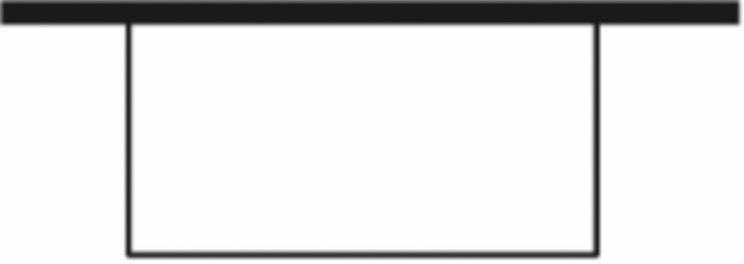
\includegraphics[width=0.28\textwidth]{figures/gao92_q8_fence.png}
\end{center}

\ifanswer
\solbegin
\step{设矩形的长为 $x$ 米，宽为 $y$，则 $xy=18$，}
\step{需要用栅栏长为 $x+2y\geqslant2\sqrt{2xy}=12$，}
\step{当且仅当 $x=2y$，即 $y=3$，$x=6$ 时取等号，故至少需要 $12$ 米栅栏.}
\solend
\fi

\item 已知 $a$ 为正整数，若关于 $x$ 的不等式 $\lvert x-2025\rvert\leqslant a$ 的解集中有且仅有 $7$ 个整数，则 $a$ 的值为\blankline[4.4em].

\ifanswer
\solbegin
\step{不等式 $\lvert x-2025\rvert\leqslant a$，则 $-a\leqslant x-2025\leqslant a$，即 $2025-a\leqslant x\leqslant2025+a$，}
\step{所以不等式 $\lvert x-2025\rvert\leqslant a$ 的解集为 $\{x\mid2025-a\leqslant x\leqslant2025+a\}$，}
\step{若不等式解集中有且仅有 $7$ 个整数，且 $a$ 为正整数，}
\step{由解集的对称性得这 $7$ 个整数以 $2025$ 为中心，向左右两边各延伸 $3$ 个整数，}
\step{即这 $7$ 个整数为 $2022,2023,2024,2025,2026,2027,2028$，所以 $a=3$.}
\solend
\fi

\item 已知关于 $x$ 的一元二次方程 $x^2-x+a=0$ 有两个不相等的正根 $m$、$n$，则 $\dfrac1m+\dfrac9n$ 的最小值为\blankline[4.4em].

\ifanswer
\solbegin
\step{因为一元二次方程 $x^2-x+a=0$ 有两个不相等的正根 $m$、$n$，}
\step{所以判别式 $\Delta=(-1)^2-4a>0\Rightarrow a<\dfrac14$，$m+n=1$，$mn=a>0$，}
\step{因此 $0<a<\dfrac14$ 且 $m+n=1(m,n>0)$.}
\step{$\dfrac1m+\dfrac9n=\left(\dfrac1m+\dfrac9n\right)(m+n)=1+\dfrac nm+\dfrac{9m}{n}+9=10+\dfrac nm+\dfrac{9m}{n}\geqslant10+2\sqrt9=16$，}
\step{等号成立条件为 $\dfrac nm=\dfrac{9m}{n}\Rightarrow n^2=9m^2\Rightarrow n=3m$，}
\step{$m$、$n>0$，结合 $m+n=1$，代入 $n=3m$ 得 $m+3m=1\Rightarrow m=\dfrac14$，$n=\dfrac34$，}
\step{此时 $mn=\dfrac14\cdot\dfrac34=\dfrac3{16}$，满足 $0<a<\dfrac14$，等号可取，因此 $\dfrac1m+\dfrac9n$ 的最小值为 $16$.}
\solend
\fi

\item 对任意 $A$、$B\subseteq R$，记 $A\oplus B=\{x\mid x\in A\cup B,x\notin A\cap B\}$，并称 $A\oplus B$ 为集合 $A$，$B$ 的对称差. 例如：若 $A=\{1,2,3\},B=\{2,3,4\}$，则 $A\oplus B=\{1,4\}$. 下列命题中，为真命题的有\blankline[4.4em].

①若 $A$、$B\subseteq R$ 且 $A\oplus B\subseteq A$，则 $A\subseteq B$

②若 $A$、$B\subseteq R$ 且 $A\oplus B=\varnothing$，则 $A=B$

③若 $A$、$B\subseteq R$ 且 $A\oplus B=B$，则 $A=\varnothing$

④对任意 $A$、$B\subseteq R$，都有 $A\oplus B=\complement_{R}A\oplus\complement_{R}B$

\ifanswer
\solbegin
\step{对于①，因为 $A\oplus B\subseteq A$，所以 $\{x\mid x\in A\cup B,x\notin A\cap B\}\subseteq A$，故 $B\subseteq A$，}
\step{故①错误；}
\step{对于②，$A$、$B\subseteq R$ 且 $A\oplus B=\varnothing$，则 $\varnothing=\{x\mid x\in A\cup B,x\notin A\cap B\}$，}
\step{即 $A\cup B=A\cap B$，所以 $A=B$，故②正确；}
\step{对于③，$A$、$B\subseteq R$ 且 $A\oplus B=B$，则 $B=\{x\mid x\in A\cup B,x\notin A\cap B\}$，}
\step{故 $A\subseteq B$，且 $B$ 中元素不在 $A\cap B$ 中，故 $A=\varnothing$，故③正确；}
\step{对于④，$\complement_{R}A\oplus\complement_{R}B=\{x\mid x\in\complement_{R}A\cup\complement_{R}B,x\notin\complement_{R}A\cap\complement_{R}B\}$，}
\step{其中 $\complement_{R}A\cup\complement_{R}B=\complement_{R}(A\cap B)$，$\complement_{R}A\cap\complement_{R}B=\complement_{R}(A\cup B)$，}
\step{故 $\complement_{R}A\oplus\complement_{R}B=\{x\mid x\in\complement_{R}(A\cap B)$，}
\step{$x\notin\complement_{R}(A\cup B)\}=\{x\mid x\in A\cup B,x\notin A\cap B\}$，}
\step{而 $A\oplus B=\{x\mid x\in A\cup B,x\notin A\cap B\}$，故 $A\oplus B=\complement_{R}A\oplus\complement_{R}B$，故④正确.}
\step{故正确的是②③④.}
\solend
\fi

\item 若不等式 $x^2-2ax+a^2-1\geqslant0$ 对任意 $x\in[0,2]$ 恒成立，则实数 $a$ 的取值范围是\blankline[4.4em].

\ifanswer
\solbegin
\step{由题意不等式 $x^2-2ax+a^2-1\geqslant0$ 对任意 $x\in[0,2]$ 恒成立，}
\step{解得 $x\leqslant a-1$ 或 $x\geqslant a+1$，要使此不等式对任意 $x\in[0,2]$ 恒成立，}
\step{则区间 $[0,2]$ 必须完全包含在解集 $(-\infty,a-1]\cup[a+1,+\infty)$ 中，}
\step{等价于 $[0,2]$ 与开区间 $(a-1,a+1)$ 的交集为空集，}
\step{区间 $[0,2]$ 在 $a-1$ 左侧，即 $2\leqslant a-1$，解得 $a\geqslant3$，}
\step{区间 $[0,2]$ 在 $a+1$ 右侧，即 $a+1\leqslant0$，解得 $a\leqslant-1$，}
\step{当 $a\in(-1,3)$，则 $(a-1,a+1)$ 与 $[0,2]$ 必有交集，不满足条件，}
\step{综上，实数 $a$ 的取值范围是 $(-\infty,-1]\cup[3,+\infty)$.}
\solend
\fi

\end{enumerate}

\bigsec{二、选择题}

\begin{enumerate}
\setcounter{enumi}{12}

\item 若 $a<b<0$，则下列不等式成立的是\mbox{（\quad）}% 原卷括号内已印“D”，试卷版按惯例留空

\keepwithprev
A. $a^2<b^2$\qquad B. $\dfrac1a<\dfrac1b$\qquad C. $ab<b^2$\qquad D. $ab<a^2$

\ifanswer
\ans{$D$}
\fi

\item 已知全集 $U=\{1,2,3,4,5\}$，集合 $A,B$ 是 $U$ 子集，满足 $\overline{A\cup B}=\{4,5\}$，$B=\{2,3\}$，则 $A\cap\overline B=\mbox{（\quad）}$

\keepwithprev
A. $\{1\}$\qquad B. $\{1,2\}$\qquad C. $\{1,4,5\}$\qquad D. $\varnothing$

\ifanswer
\solbegin
\step{因为全集 $U=\{1,2,3,4,5\}$，集合 $A$、$B$ 是 $U$ 子集，$\overline{A\cup B}=\{4,5\}$，$B=\{2,3\}$，}
\step{所以 $A\cup B=\{1,2,3\}$，故 $1\in A$，$1\notin B$，$4\notin A$，$5\notin A$，$4\notin B$，$5\notin B$，}
\step{故 $A\cap\overline B=\{1\}$. 故选 $A$.}
\solend
\fi

\item 设 $a>0$，若关于 $x$ 的不等式 $x^2-(2a-1)x-2a<0$ 的解集中恰有 $3$ 个整数，则实数 $a$ 的取值范围是\mbox{（\quad）}

\keepwithprev
A. $\left[1,\dfrac32\right]$\qquad B. $\left(1,\dfrac32\right]$\qquad C. $\left[\dfrac12,1\right]$\qquad D. $\left(\dfrac12,1\right]$

\ifanswer
\solbegin
\step{已知关于 $x$ 的不等式 $x^2-(2a-1)x-2a<0$，则 $(x+1)(x-2a)<0$，}
\step{则 $-1<x<2a$，又解集中恰有 $3$ 个整数，则 $2<2a\leqslant3$，则 $1<a\leqslant\dfrac32$，}
\step{则 $a$ 的取值范围为 $\left(1,\dfrac32\right]$. 故选 $B$.}
\solend
\fi

\item 已知集合 $U=\{1,2,3,\cdots,2027\}$，$M\subseteq U$，若对于 $M$ 中的任意两个不同的元素 $x$、$y$，都有 $\lvert x-y\rvert>2$，则 $M$ 中元素个数的最大值为\mbox{（\quad）}

\keepwithprev
A. $675$\qquad B. $676$\qquad C. $2025$\qquad D. $2026$

\ifanswer
\solbegin
\step{对于 $M$ 中的任意两个不同的元素 $x$、$y$，都有 $\lvert x-y\rvert>2$，}
\step{不妨设 $x>y$，都有 $x-y\geqslant3$，}
\step{要想 $M$ 所含元素个数最大，则要 $x-y$ 尽可能小，故需使得 $x-y$ 的最小值为 $3$，}
\step{将 $1\sim2027$ 这 $2027$ 个元素按如下分组：}
\step{$\{1,2,3\},\{4,5,6\},\cdots,\{2023,2024,2025\},\{2026,2027\}$，}
\step{故应在前 $675$ 组中按周期 $3$ 每组取一个元素，且第一组中不能取 $3$，}
\step{第一组中取 $1$ 时，得 $M=\{1,4,7,\cdots,2023,2026\}$}
\step{或 $M=\{1,4,7,\cdots,2023,2027\}$ 这样的集合，}
\step{第一组取 $2$ 时，得 $M=\{2,5,8,\cdots,2024,2027\}$，}
\step{其中任意两元素差值 $x-y(x>y)$ 都大于 $2$，满足题意，}
\step{故 $M$ 所含元素个数的最大值为 $\dfrac{2025}{3}+1=676$. 故选 $B$.}
\solend
\fi

\end{enumerate}

\bigsec{三、解答题}

\begin{enumerate}
\setcounter{enumi}{16}

\item 已知集合 $M=\{x\mid a-1\leqslant x\leqslant2a+3\}$，$P=\{x\mid-2<x\leqslant4\}$，全集 $U=R$.

（1）当 $a=2$ 时，求 $M\cap P$；

（2）若 $x\in P$ 是 $x\in M$ 的必要不充分条件，求实数 $a$ 的取值范围.

\ansspace*[9]

\ifanswer
\solbegin
\stepm{（1）}{当 $a=2$ 时，集合 $M=\{x\mid1\leqslant x\leqslant7\}$，所以 $M\cap P=\{x\mid1\leqslant x\leqslant4\}$；}
\stepm{（2）}{因为 $x\in P$ 是 $x\in M$ 的必要不充分条件，所以 $M\subsetneqq P$，}
\step{当 $M=\varnothing$ 时，$a-1>2a+3$，解得 $a<-4$，}
\step{当 $M\neq\varnothing$ 时，则 $\begin{cases}a-1\leqslant2a+3\\ a-1>-2\\ 2a+3\leqslant4\end{cases}$，解得 $-1<a\leqslant\dfrac12$，}
\step{综上所述，实数 $a$ 的取值范围为 $(-\infty,-4)\cup\left(-1,\dfrac12\right]$.}
\solend
\fi

\item 命题甲：关于 $x$ 的方程 $(a-1)x^2+(2a-4)x+a=0$ 有两个不相等的实数根；

命题乙：关于 $x$ 的不等式 $ax^2-2ax+a+1>0$ 的解集为 $R$.

（1）若命题甲为真命题，求实数 $a$ 的取值范围；

（2）若命题甲、乙中至多有一个为真命题，求实数 $a$ 的取值范围.

\ansspace*[12]

\ifanswer
\solbegin
\stepm{（1）}{命题甲：关于 $x$ 的方程 $(a-1)x^2+(2a-4)x+a=0$ 有两个不相等的实数根，}
\step{则 $\begin{cases}a-1\neq0\\ \Delta=(2a-4)^2-4a(a-1)>0\end{cases}$，解得 $a<\dfrac43$ 且 $a\neq1$，}
\step{故 $a$ 的范围为 $\left\{a\left|a<\dfrac43\ \text{且}\ a\neq1\right.\right\}$；}
\stepm{（2）}{当 $a=0$ 时 $y=1>0$，符合题意；}
\step{当 $a\neq0$，由 $\begin{cases}a>0\\ \Delta=4a^2-4a(a+1)<0\end{cases}$，解得 $a>0$，}
\step{则 $a$ 的取值范围为 $a\geqslant0$，}
\step{故 $p$、$q$ 都为真时，$a$ 的范围为 $0\leqslant a<\dfrac43$ 且 $a\neq1$，}
\step{则命题甲、乙中至多有一个为真命题时，}
\step{$a$ 的取值范围为 $\left\{a\left|a<0\ \text{或}\ a=1\ \text{或}\ a\geqslant\dfrac43\right.\right\}$.}
\solend
\fi

\item 如图，$OA$、$OB$ 是两条长度足够长的互相垂直的笔直小路，矩形 $OCPD$ 的顶点 $C$，$D$ 分别在 $OA$、$OB$ 上，且该矩形区域内种满了荷花. 为了让观赏者有更好的观赏体验，现计划经过点 $P$ 修一条小路 $EF$，其中点 $E$ 在小路 $OA$ 上，点 $F$ 在小路 $OB$ 上，并在 $\triangle OEF$ 区域内种满荷花. 已知 $OD=25$ m，$OC=40$ m，且小路 $EF$ 要完全位于一个以 $O$ 为顶点的，边长为 $100$ m 的正方形内部（包括边界）. 记 $\triangle OEF$ 的面积为 $S$ m$^2$.

\begin{center}
\begin{tikzpicture}[x=0.46cm,y=0.42cm,line width=0.7pt]
\draw (0,0) -- (0,10.2) node[above,inner sep=3pt] {$A$};
\draw (0,0) -- (11.8,0) node[right,inner sep=3pt] {$B$};
\draw (0,4.83) -- (2.42,4.83) -- (2.42,0);
\draw (0,6.92) -- (8.01,0);
\node[below left,inner sep=2pt] at (0,0) {$O$};
\node[below,inner sep=2pt] at (2.42,0) {$D$};
\node[left,inner sep=3pt] at (0,4.83) {$C$};
\node[above right,inner sep=1pt] at (2.42,4.83) {$P$};
\node[left,inner sep=3pt] at (0,6.92) {$E$};
\node[below,inner sep=2pt] at (8.01,0) {$F$};
\end{tikzpicture}
\end{center}

（1）设 $EC=x\cdot m$，试用 $x$ 表示 $OF$，并求 $x$ 的取值范围.

（2）当 $EC$ 的长度为多少时，$S$ 取得最小值？最小值是多少？

\ansspace*[11]

\ifanswer
\solbegin
\stepm{（1）}{由题意得 $x\leqslant60$，}
\step{$\triangle PCE\backsim\triangle FDP$，所以 $\dfrac{EC}{CP}=\dfrac{PD}{DF}$，即 $\dfrac{x}{25}=\dfrac{40}{DF}$，得 $DF=\dfrac{1000}{x}$ m，}
\step{所以 $OF=OD+DF=\left(25+\dfrac{1000}{x}\right)$ m，}
\step{所以 $25+\dfrac{1000}{x}\leqslant100$，解得 $x\geqslant\dfrac{40}{3}$；}
\step{综上，$\dfrac{40}{3}\leqslant x\leqslant60$；}
\stepm{（2）}{由 $OE=OC+CE=(40+x)$ m，}
\step{所以 $S=\dfrac12\cdot OF\cdot OE=\dfrac12\left(25+\dfrac{1000}{x}\right)(40+x)$}
\step{$=\dfrac12\left(1000+25x+\dfrac{40000}{x}+1000\right)$ m$^2$，}
\step{由基本不等式得 $S\geqslant\dfrac12\left(2000+2\sqrt{25x\cdot\dfrac{40000}{x}}\right)=2000$ m$^2$，}
\step{当且仅当 $25x=\dfrac{40000}{x}$，即 $x=40$ 时取等号，}
\step{故 $EC=40$ m 时，$S$ 取得最小值，为 $2000$ m$^2$.}
\solend
\fi

\item 已知函数 $f(x)=x^2-(a-2)x+a-3$.

（1）若 $f(x)=0$ 的两根为 $\alpha,\beta$，$\alpha^2+\beta^2=2$，求 $a$ 的值；

（2）解关于 $x$ 的不等式 $f(x)\geqslant0$；

（3）是否存在整数 $m,n$，使得关于 $x$ 的不等式 $m\leqslant f(x)\leqslant n$ 的解集恰好为 $[m,n]$？若存在，求出 $m,n$ 的值. 若不存在，请说明理由.

\ansspace*[16]

\ifanswer
\solbegin
\stepm{（1）}{由韦达定理，$\alpha+\beta=a-2,\alpha\beta=a-3$，}
\step{因此 $\alpha^2+\beta^2=(a-2)^2-2(a-3)=2\Leftrightarrow(a-2)(a-4)=0$，}
\step{$a=2$ 时两根为 $1,-1$；$a=4$ 时两根均为 $1$，均满足条件，}
\step{所以 $a=2$ 或 $a=4$.}
\stepm{（2）}{因为 $f(x)=(x-1)[x-(a-3)]$，所以分三种情况：}
\step{当 $a<4$ 时，$a-3<1$，解集为 $(-\infty,a-3]\cup[1,+\infty)$.}
\step{当 $a=4$ 时，$f(x)=(x-1)^2\geqslant0$ 恒成立，解集为 $R$.}
\step{当 $a>4$ 时，$a-3>1$，解集为 $(-\infty,1]\cup[a-3,+\infty)$.}
\stepm{（3）}{区间 $[m,n]$ 要求 $m<n$. 记 $f(x)$ 的最小值为 $k$.}
\step{$[m,n]$ 非空，不等式 $f(x)\leqslant n$ 有解，其解集为闭区间 $[x_1,x_2]$，}
\step{其中 $x_1\leqslant x_2$ 是方程 $f(x)=n$ 的两根.}
\step{若 $k<m$，则 $f(x)<m$ 的解集是 $[x_1,x_2]$ 内部的一个开区间，}
\step{从 $[x_1,x_2]$ 中去掉它后剩下两段，原不等式的解集不是一个区间，矛盾，}
\step{所以 $k\geqslant m$，原不等式的解集就是 $[x_1,x_2]$，于是 $m=x_1,n=x_2$，}
\step{即 $f(m)=f(n)=n$，于是 $f(m)-f(n)=(m-n)(m+n-a+2)=0$.}
\step{因为 $m\neq n$，所以 $a=m+n+2$.}
\step{代入 $f(m)=n$，得 $(m-1)(1-n)=n\Leftrightarrow m(n-1)=-1$，$m,n$ 均为整数，}
\step{因此 $(m,n)=(-1,2)$ 或 $(m,n)=(1,0)$.}
\step{结合 $m<n$，只可能有 $m=-1,n=2$，此时 $a=3$.}
\step{检验：此时 $f(x)=x^2-x$，且 $x^2-x=\left(x-\dfrac12\right)^2-\dfrac14\geqslant-\dfrac14>-1$，}
\step{因此 $-1\leqslant f(x)\leqslant2\Leftrightarrow x^2-x\leqslant2\Leftrightarrow(x+1)(x-2)\leqslant0\Leftrightarrow x\in[-1,2]$，}
\step{所以存在符合条件的整数 $m=-1,n=2$.}
\solend
\fi

\item 给定数集 $M$，若对于任意 $a$、$b\in M$，有 $a+b\in M,a-b\in M$，则称集合 $M$ 为闭集合.

（1）判断集合 $A_1=\{-4,-2,0,2,4\}$，集合 $B=\{x\mid x=3k,k\in\Z\}$ 是否为闭集合；

（2）若集合 $C$、$D$ 为闭集合，则 $C\cup D$ 是否一定为闭集合？请说明理由；

（3）已知集合 $C$、$D$ 为闭集合，且 $C\subsetneq R,D\subsetneq R$，证明：$(C\cup D)\subsetneq R$.% 原卷印作 (C∪D)⊂R，按解析证明的是 C∪D≠R，排真子集

\ansspace*[14]

\ifanswer
\solbegin
\stepm{（1）}{因为 $4\in A_1$，$2\in A_1$，$4+2=6\notin A_1$，所以 $A_1$ 不是闭集合；}
\step{任取 $x,y\in B$，设 $x=3m,y=3n,m,n\in\Z$，}
\step{则 $x+y=3m+3n=3(m+n)$ 且 $m+n\in\Z$，}
\step{所以 $x+y\in B$，同理，$x-y\in B$，故 $B$ 为闭集合.}
\stepm{（2）}{结论：不一定.}
\step{不妨令 $C=\{x\mid x=2k,k\in\Z\},D=\{x\mid x=3k,k\in\Z\}$，}
\step{则由（1）得 $C$、$D$ 为闭集合，易得 $2,3\in C\cup D,2+3=5\notin C\cup D$，}
\step{因此，$C\cup D$ 不一定是闭集合.}
\stepm{（3）}{不妨假设 $C\cup D=R$，则由 $C\subsetneq R$，得存在 $a\in R$ 且 $a\notin C$，故 $a\in D$.}
\step{同理，存在 $b\in R$ 且 $b\notin D$，故 $b\in C$.}
\step{因为 $a+b\in R=C\cup D$，所以 $a+b\in C$ 或 $a+b\in D$.}
\step{若 $a+b\in C$，则由 $C$ 为闭集合且 $b\in C$，得 $a=(a+b)-b\in C$，}
\step{与 $a\notin C$ 矛盾.}
\step{若 $a+b\in D$，则由 $D$ 为闭集合且 $a\in D$，得 $b=(a+b)-a\in D$，}
\step{与 $b\notin D$ 矛盾.}
\step{综上，$C\cup D=R$ 不成立，故 $(C\cup D)\subsetneq R$.}
\solend
\fi

\end{enumerate}

\end{document}
"
% 紧凑版：xelatex "\def\iscompact{1}% 高一92_闵行实验_10月月考.tex
%   —— 高一上数学“2026-2027 年闵行实验高一上 10 月月考”（讲评版）
% 试卷版：xelatex 高一92_闵行实验_10月月考.tex
% 答案版：xelatex "\def\isanswer{1}% 高一92_闵行实验_10月月考.tex
%   —— 高一上数学“2026-2027 年闵行实验高一上 10 月月考”（讲评版）
% 试卷版：xelatex 高一92_闵行实验_10月月考.tex
% 答案版：xelatex "\def\isanswer{1}\input{高一92_闵行实验_10月月考.tex}"
% 紧凑版：xelatex "\def\iscompact{1}\input{高一92_闵行实验_10月月考.tex}"
%
% 原始材料：微信公众号“魔都数学加油站”文章，连载“27学年高一92”；
% 原文标题“27学年高一92——2026-2027年上海市闵行实验高一上10月月考”；
% 原文链接：https://mp.weixin.qq.com/s/8HUyr3G7GpcHyczwu_XYCQ。
% 正文为 10 张 PNG 页（`原图/高一92_闵行实验_10月月考/01..10.png`），均 4762×6735，按页序读取。
%
% 篇幅与题号：原卷自第 3 题起编号（第 1、2 题不在原文内）。填空题 3—12（10 题）、
% 选择题 13—16（4 题）、解答题 17—21（5 题），共 19 题。
%
% 讲评版：第 6 题只印【答案】（“$[-1,3]$”），本稿只给 \ans{}；第 13 题无【解析】、
% 答案“D”直接印在题干括号内，本稿试卷版按惯例留空、答案版提 \ans{$D$}；其余 17 题印
% 【解析】，其中选择题答案在解析末句“故选 $A$／$B$／$B$”。
% 第 8 题题干右侧有一幅“围墙 + 三面栅栏”示意图（裁自第 2 页原图）；第 19 题题干带
% 与 高一88 第 19 题同型的示意图（$OA$／$OB$ 两条小路、矩形 $OCPD$、折线 $EF$），用 TikZ 重绘。
%
% 副标题：原卷未印副标题。本稿按内容标作“集合与常用逻辑用语、不等式”。
%
% 原卷笔误/存疑（均照录未改，正文对应处另有 % 注）：
%   ① 第 21 题 (3) 题干与解析末句把结论印作“$(C\cup D)\subset R$”，而解析证明的是
%      “$C\cup D=\R$ 不成立”，按文意应为“$(C\cup D)\subsetneq\R$”；本稿按真子集排
%      $\subsetneq$，原卷记号照录于文件头；
%   ② 第 7 题解析只列 $B=\varnothing$（$a=0$）、$B=\{1\}$（$a=1$）、$B=\{-3\}$（$a=-\frac13$）
%      三种情形，与结论 $\left\{0,1,-\frac13\right\}$ 相符，无笔误。
%
% 与原卷的排版差异：
%   ① 原卷每题下直接印【答案】/【解析】，本稿按全稿惯例将答案与解析置于答案版；
%   ② 原卷未印副标题，本稿补出；填空横线统一排 \blankline[4.4em]；
%   ③ 原卷数集记号排斜体 $R$、$Z$，本稿按全稿惯例改用 $\R$、$\Z$；
%   ④ 第 17—21 题的子问用行内“（1）（2）（3）”段，解析中的子问标号用 \stepm；
%   ⑤ 解答题按惯例加 \ansspace；选择题括号排 \mbox{（\quad）}；
%   ⑥ 第 8 题的示意图原卷排在题干右侧、文字绕排，本稿改排为题干后的居中图
%      （自原图裁切、去粉色水印后转灰度）；第 19 题的图按原图比例 TikZ 重绘。
%
% 行数核对：逐题数 \step/\stepm 条数，合计 128 条（Q3：2；Q4：3；Q5：2；Q6：0；Q7：6；
% Q8：3；Q9：5；Q10：7；Q11：12；Q12：8；Q13：0；Q14：3；Q15：3；Q16：11；Q17：5；
% Q18：9；Q19：11；Q20：22；Q21：16）。第 6 题只印答案、第 13 题无解析，均不计入 \step 账。
% 原卷解析的换行按语意合并，未逐行强拆。
%
\documentclass[a4paper,11pt]{article}
\usepackage{common}

\begin{document}

\examtitlest[7]{2026--2027 年闵行实验高一上 10 月月考}{集合与常用逻辑用语、不等式}

\bigsec{一、填空题}

\begin{enumerate}
\setcounter{enumi}{2}

\item 已知 $3<a<8$，$4<b<9$，则 $\dfrac ab$ 的取值范围是\blankline[4.4em].

\ifanswer
\solbegin
\step{因为 $4<b<9$，所以 $\dfrac19<\dfrac1b<\dfrac14$，又 $3<a<8$，所以 $\dfrac13<\dfrac ab<2$，}
\step{故 $\dfrac ab$ 的取值范围是 $\left(\dfrac13,2\right)$.}
\solend
\fi

\item 已知 $p:x>3$，$q:x>5$，则 $p$ 是 $q$ 的\blankline[4.4em]（选“充分不必要条件”“必要不充分条件”“充要条件”“既不充分也不必要条件”之一填空）.

\ifanswer
\solbegin
\step{当 $x>3$ 时，不能推出 $x>5$，充分性不成立；}
\step{当 $x>5$ 时，可以得到 $x>3$，必要性成立；}
\step{故 $p$ 是 $q$ 的必要不充分条件.}
\solend
\fi

\item 不等式 $\dfrac{x-1}{2x+1}\leqslant1$ 的解集为\blankline[4.4em].

\ifanswer
\solbegin
\step{因为 $\dfrac{x-1}{2x+1}\leqslant1$，所以 $\dfrac{x-1}{2x+1}-\dfrac{2x+1}{2x+1}\leqslant0$，所以 $\dfrac{x+2}{2x+1}\geqslant0$，}
\step{所以 $x>-\dfrac12$ 或 $x\leqslant-2$，即不等式的解集是 $(-\infty,-2]\cup\left(-\dfrac12,+\infty\right)$.}
\solend
\fi

\item 设 $x\in R$，则方程 $\lvert x+1\rvert+\lvert x-3\rvert=4$ 的解集为\blankline[4.4em].

\ifanswer
\ans{$[-1,3]$}
\fi

\item 若 $A=\{x\mid x^2+2x=3\}$，$B=\{x\mid ax=1\}$，且 $B\subseteq A$，则实数 $a$ 的值组成的集合为\blankline[4.4em].

\ifanswer
\solbegin
\step{由 $x^2+2x=3$ 得 $x^2+2x-3=0$，解得 $x=1$ 或 $x=-3$，所以 $A=\{1,-3\}$，}
\step{又因为 $B=\{x\mid ax=1\}$，且 $B\subseteq A$，}
\step{当 $B=\varnothing$，即 $a=0$ 时，显然符合题意；}
\step{当 $B=\{1\}$，即 $a=1$ 时，也符合题意；}
\step{当 $B=\{-3\}$，即 $a=-\dfrac13$ 时，也符合题意；}
\step{综上所述，实数 $a$ 的值组成的集合为 $\left\{0,1,-\dfrac13\right\}$.}
\solend
\fi

\item 某校欲在围墙边用栅栏围成一个 $18$ 平方米的矩形区域，作为天鹅的地面栖息地，矩形区域的一条边为围墙（如图），则至少需要\blankline[4.4em]米栅栏.

\begin{center}
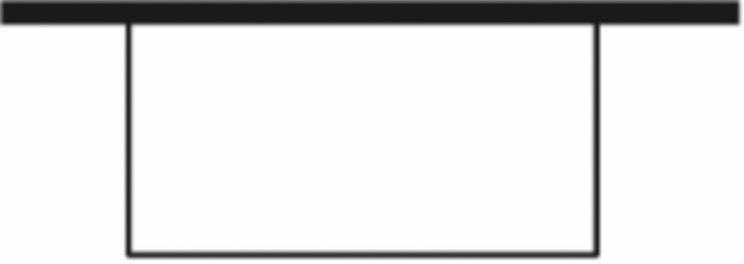
\includegraphics[width=0.28\textwidth]{figures/gao92_q8_fence.png}
\end{center}

\ifanswer
\solbegin
\step{设矩形的长为 $x$ 米，宽为 $y$，则 $xy=18$，}
\step{需要用栅栏长为 $x+2y\geqslant2\sqrt{2xy}=12$，}
\step{当且仅当 $x=2y$，即 $y=3$，$x=6$ 时取等号，故至少需要 $12$ 米栅栏.}
\solend
\fi

\item 已知 $a$ 为正整数，若关于 $x$ 的不等式 $\lvert x-2025\rvert\leqslant a$ 的解集中有且仅有 $7$ 个整数，则 $a$ 的值为\blankline[4.4em].

\ifanswer
\solbegin
\step{不等式 $\lvert x-2025\rvert\leqslant a$，则 $-a\leqslant x-2025\leqslant a$，即 $2025-a\leqslant x\leqslant2025+a$，}
\step{所以不等式 $\lvert x-2025\rvert\leqslant a$ 的解集为 $\{x\mid2025-a\leqslant x\leqslant2025+a\}$，}
\step{若不等式解集中有且仅有 $7$ 个整数，且 $a$ 为正整数，}
\step{由解集的对称性得这 $7$ 个整数以 $2025$ 为中心，向左右两边各延伸 $3$ 个整数，}
\step{即这 $7$ 个整数为 $2022,2023,2024,2025,2026,2027,2028$，所以 $a=3$.}
\solend
\fi

\item 已知关于 $x$ 的一元二次方程 $x^2-x+a=0$ 有两个不相等的正根 $m$、$n$，则 $\dfrac1m+\dfrac9n$ 的最小值为\blankline[4.4em].

\ifanswer
\solbegin
\step{因为一元二次方程 $x^2-x+a=0$ 有两个不相等的正根 $m$、$n$，}
\step{所以判别式 $\Delta=(-1)^2-4a>0\Rightarrow a<\dfrac14$，$m+n=1$，$mn=a>0$，}
\step{因此 $0<a<\dfrac14$ 且 $m+n=1(m,n>0)$.}
\step{$\dfrac1m+\dfrac9n=\left(\dfrac1m+\dfrac9n\right)(m+n)=1+\dfrac nm+\dfrac{9m}{n}+9=10+\dfrac nm+\dfrac{9m}{n}\geqslant10+2\sqrt9=16$，}
\step{等号成立条件为 $\dfrac nm=\dfrac{9m}{n}\Rightarrow n^2=9m^2\Rightarrow n=3m$，}
\step{$m$、$n>0$，结合 $m+n=1$，代入 $n=3m$ 得 $m+3m=1\Rightarrow m=\dfrac14$，$n=\dfrac34$，}
\step{此时 $mn=\dfrac14\cdot\dfrac34=\dfrac3{16}$，满足 $0<a<\dfrac14$，等号可取，因此 $\dfrac1m+\dfrac9n$ 的最小值为 $16$.}
\solend
\fi

\item 对任意 $A$、$B\subseteq R$，记 $A\oplus B=\{x\mid x\in A\cup B,x\notin A\cap B\}$，并称 $A\oplus B$ 为集合 $A$，$B$ 的对称差. 例如：若 $A=\{1,2,3\},B=\{2,3,4\}$，则 $A\oplus B=\{1,4\}$. 下列命题中，为真命题的有\blankline[4.4em].

①若 $A$、$B\subseteq R$ 且 $A\oplus B\subseteq A$，则 $A\subseteq B$

②若 $A$、$B\subseteq R$ 且 $A\oplus B=\varnothing$，则 $A=B$

③若 $A$、$B\subseteq R$ 且 $A\oplus B=B$，则 $A=\varnothing$

④对任意 $A$、$B\subseteq R$，都有 $A\oplus B=\complement_{R}A\oplus\complement_{R}B$

\ifanswer
\solbegin
\step{对于①，因为 $A\oplus B\subseteq A$，所以 $\{x\mid x\in A\cup B,x\notin A\cap B\}\subseteq A$，故 $B\subseteq A$，}
\step{故①错误；}
\step{对于②，$A$、$B\subseteq R$ 且 $A\oplus B=\varnothing$，则 $\varnothing=\{x\mid x\in A\cup B,x\notin A\cap B\}$，}
\step{即 $A\cup B=A\cap B$，所以 $A=B$，故②正确；}
\step{对于③，$A$、$B\subseteq R$ 且 $A\oplus B=B$，则 $B=\{x\mid x\in A\cup B,x\notin A\cap B\}$，}
\step{故 $A\subseteq B$，且 $B$ 中元素不在 $A\cap B$ 中，故 $A=\varnothing$，故③正确；}
\step{对于④，$\complement_{R}A\oplus\complement_{R}B=\{x\mid x\in\complement_{R}A\cup\complement_{R}B,x\notin\complement_{R}A\cap\complement_{R}B\}$，}
\step{其中 $\complement_{R}A\cup\complement_{R}B=\complement_{R}(A\cap B)$，$\complement_{R}A\cap\complement_{R}B=\complement_{R}(A\cup B)$，}
\step{故 $\complement_{R}A\oplus\complement_{R}B=\{x\mid x\in\complement_{R}(A\cap B)$，}
\step{$x\notin\complement_{R}(A\cup B)\}=\{x\mid x\in A\cup B,x\notin A\cap B\}$，}
\step{而 $A\oplus B=\{x\mid x\in A\cup B,x\notin A\cap B\}$，故 $A\oplus B=\complement_{R}A\oplus\complement_{R}B$，故④正确.}
\step{故正确的是②③④.}
\solend
\fi

\item 若不等式 $x^2-2ax+a^2-1\geqslant0$ 对任意 $x\in[0,2]$ 恒成立，则实数 $a$ 的取值范围是\blankline[4.4em].

\ifanswer
\solbegin
\step{由题意不等式 $x^2-2ax+a^2-1\geqslant0$ 对任意 $x\in[0,2]$ 恒成立，}
\step{解得 $x\leqslant a-1$ 或 $x\geqslant a+1$，要使此不等式对任意 $x\in[0,2]$ 恒成立，}
\step{则区间 $[0,2]$ 必须完全包含在解集 $(-\infty,a-1]\cup[a+1,+\infty)$ 中，}
\step{等价于 $[0,2]$ 与开区间 $(a-1,a+1)$ 的交集为空集，}
\step{区间 $[0,2]$ 在 $a-1$ 左侧，即 $2\leqslant a-1$，解得 $a\geqslant3$，}
\step{区间 $[0,2]$ 在 $a+1$ 右侧，即 $a+1\leqslant0$，解得 $a\leqslant-1$，}
\step{当 $a\in(-1,3)$，则 $(a-1,a+1)$ 与 $[0,2]$ 必有交集，不满足条件，}
\step{综上，实数 $a$ 的取值范围是 $(-\infty,-1]\cup[3,+\infty)$.}
\solend
\fi

\end{enumerate}

\bigsec{二、选择题}

\begin{enumerate}
\setcounter{enumi}{12}

\item 若 $a<b<0$，则下列不等式成立的是\mbox{（\quad）}% 原卷括号内已印“D”，试卷版按惯例留空

\keepwithprev
A. $a^2<b^2$\qquad B. $\dfrac1a<\dfrac1b$\qquad C. $ab<b^2$\qquad D. $ab<a^2$

\ifanswer
\ans{$D$}
\fi

\item 已知全集 $U=\{1,2,3,4,5\}$，集合 $A,B$ 是 $U$ 子集，满足 $\overline{A\cup B}=\{4,5\}$，$B=\{2,3\}$，则 $A\cap\overline B=\mbox{（\quad）}$

\keepwithprev
A. $\{1\}$\qquad B. $\{1,2\}$\qquad C. $\{1,4,5\}$\qquad D. $\varnothing$

\ifanswer
\solbegin
\step{因为全集 $U=\{1,2,3,4,5\}$，集合 $A$、$B$ 是 $U$ 子集，$\overline{A\cup B}=\{4,5\}$，$B=\{2,3\}$，}
\step{所以 $A\cup B=\{1,2,3\}$，故 $1\in A$，$1\notin B$，$4\notin A$，$5\notin A$，$4\notin B$，$5\notin B$，}
\step{故 $A\cap\overline B=\{1\}$. 故选 $A$.}
\solend
\fi

\item 设 $a>0$，若关于 $x$ 的不等式 $x^2-(2a-1)x-2a<0$ 的解集中恰有 $3$ 个整数，则实数 $a$ 的取值范围是\mbox{（\quad）}

\keepwithprev
A. $\left[1,\dfrac32\right]$\qquad B. $\left(1,\dfrac32\right]$\qquad C. $\left[\dfrac12,1\right]$\qquad D. $\left(\dfrac12,1\right]$

\ifanswer
\solbegin
\step{已知关于 $x$ 的不等式 $x^2-(2a-1)x-2a<0$，则 $(x+1)(x-2a)<0$，}
\step{则 $-1<x<2a$，又解集中恰有 $3$ 个整数，则 $2<2a\leqslant3$，则 $1<a\leqslant\dfrac32$，}
\step{则 $a$ 的取值范围为 $\left(1,\dfrac32\right]$. 故选 $B$.}
\solend
\fi

\item 已知集合 $U=\{1,2,3,\cdots,2027\}$，$M\subseteq U$，若对于 $M$ 中的任意两个不同的元素 $x$、$y$，都有 $\lvert x-y\rvert>2$，则 $M$ 中元素个数的最大值为\mbox{（\quad）}

\keepwithprev
A. $675$\qquad B. $676$\qquad C. $2025$\qquad D. $2026$

\ifanswer
\solbegin
\step{对于 $M$ 中的任意两个不同的元素 $x$、$y$，都有 $\lvert x-y\rvert>2$，}
\step{不妨设 $x>y$，都有 $x-y\geqslant3$，}
\step{要想 $M$ 所含元素个数最大，则要 $x-y$ 尽可能小，故需使得 $x-y$ 的最小值为 $3$，}
\step{将 $1\sim2027$ 这 $2027$ 个元素按如下分组：}
\step{$\{1,2,3\},\{4,5,6\},\cdots,\{2023,2024,2025\},\{2026,2027\}$，}
\step{故应在前 $675$ 组中按周期 $3$ 每组取一个元素，且第一组中不能取 $3$，}
\step{第一组中取 $1$ 时，得 $M=\{1,4,7,\cdots,2023,2026\}$}
\step{或 $M=\{1,4,7,\cdots,2023,2027\}$ 这样的集合，}
\step{第一组取 $2$ 时，得 $M=\{2,5,8,\cdots,2024,2027\}$，}
\step{其中任意两元素差值 $x-y(x>y)$ 都大于 $2$，满足题意，}
\step{故 $M$ 所含元素个数的最大值为 $\dfrac{2025}{3}+1=676$. 故选 $B$.}
\solend
\fi

\end{enumerate}

\bigsec{三、解答题}

\begin{enumerate}
\setcounter{enumi}{16}

\item 已知集合 $M=\{x\mid a-1\leqslant x\leqslant2a+3\}$，$P=\{x\mid-2<x\leqslant4\}$，全集 $U=R$.

（1）当 $a=2$ 时，求 $M\cap P$；

（2）若 $x\in P$ 是 $x\in M$ 的必要不充分条件，求实数 $a$ 的取值范围.

\ansspace*[9]

\ifanswer
\solbegin
\stepm{（1）}{当 $a=2$ 时，集合 $M=\{x\mid1\leqslant x\leqslant7\}$，所以 $M\cap P=\{x\mid1\leqslant x\leqslant4\}$；}
\stepm{（2）}{因为 $x\in P$ 是 $x\in M$ 的必要不充分条件，所以 $M\subsetneqq P$，}
\step{当 $M=\varnothing$ 时，$a-1>2a+3$，解得 $a<-4$，}
\step{当 $M\neq\varnothing$ 时，则 $\begin{cases}a-1\leqslant2a+3\\ a-1>-2\\ 2a+3\leqslant4\end{cases}$，解得 $-1<a\leqslant\dfrac12$，}
\step{综上所述，实数 $a$ 的取值范围为 $(-\infty,-4)\cup\left(-1,\dfrac12\right]$.}
\solend
\fi

\item 命题甲：关于 $x$ 的方程 $(a-1)x^2+(2a-4)x+a=0$ 有两个不相等的实数根；

命题乙：关于 $x$ 的不等式 $ax^2-2ax+a+1>0$ 的解集为 $R$.

（1）若命题甲为真命题，求实数 $a$ 的取值范围；

（2）若命题甲、乙中至多有一个为真命题，求实数 $a$ 的取值范围.

\ansspace*[12]

\ifanswer
\solbegin
\stepm{（1）}{命题甲：关于 $x$ 的方程 $(a-1)x^2+(2a-4)x+a=0$ 有两个不相等的实数根，}
\step{则 $\begin{cases}a-1\neq0\\ \Delta=(2a-4)^2-4a(a-1)>0\end{cases}$，解得 $a<\dfrac43$ 且 $a\neq1$，}
\step{故 $a$ 的范围为 $\left\{a\left|a<\dfrac43\ \text{且}\ a\neq1\right.\right\}$；}
\stepm{（2）}{当 $a=0$ 时 $y=1>0$，符合题意；}
\step{当 $a\neq0$，由 $\begin{cases}a>0\\ \Delta=4a^2-4a(a+1)<0\end{cases}$，解得 $a>0$，}
\step{则 $a$ 的取值范围为 $a\geqslant0$，}
\step{故 $p$、$q$ 都为真时，$a$ 的范围为 $0\leqslant a<\dfrac43$ 且 $a\neq1$，}
\step{则命题甲、乙中至多有一个为真命题时，}
\step{$a$ 的取值范围为 $\left\{a\left|a<0\ \text{或}\ a=1\ \text{或}\ a\geqslant\dfrac43\right.\right\}$.}
\solend
\fi

\item 如图，$OA$、$OB$ 是两条长度足够长的互相垂直的笔直小路，矩形 $OCPD$ 的顶点 $C$，$D$ 分别在 $OA$、$OB$ 上，且该矩形区域内种满了荷花. 为了让观赏者有更好的观赏体验，现计划经过点 $P$ 修一条小路 $EF$，其中点 $E$ 在小路 $OA$ 上，点 $F$ 在小路 $OB$ 上，并在 $\triangle OEF$ 区域内种满荷花. 已知 $OD=25$ m，$OC=40$ m，且小路 $EF$ 要完全位于一个以 $O$ 为顶点的，边长为 $100$ m 的正方形内部（包括边界）. 记 $\triangle OEF$ 的面积为 $S$ m$^2$.

\begin{center}
\begin{tikzpicture}[x=0.46cm,y=0.42cm,line width=0.7pt]
\draw (0,0) -- (0,10.2) node[above,inner sep=3pt] {$A$};
\draw (0,0) -- (11.8,0) node[right,inner sep=3pt] {$B$};
\draw (0,4.83) -- (2.42,4.83) -- (2.42,0);
\draw (0,6.92) -- (8.01,0);
\node[below left,inner sep=2pt] at (0,0) {$O$};
\node[below,inner sep=2pt] at (2.42,0) {$D$};
\node[left,inner sep=3pt] at (0,4.83) {$C$};
\node[above right,inner sep=1pt] at (2.42,4.83) {$P$};
\node[left,inner sep=3pt] at (0,6.92) {$E$};
\node[below,inner sep=2pt] at (8.01,0) {$F$};
\end{tikzpicture}
\end{center}

（1）设 $EC=x\cdot m$，试用 $x$ 表示 $OF$，并求 $x$ 的取值范围.

（2）当 $EC$ 的长度为多少时，$S$ 取得最小值？最小值是多少？

\ansspace*[11]

\ifanswer
\solbegin
\stepm{（1）}{由题意得 $x\leqslant60$，}
\step{$\triangle PCE\backsim\triangle FDP$，所以 $\dfrac{EC}{CP}=\dfrac{PD}{DF}$，即 $\dfrac{x}{25}=\dfrac{40}{DF}$，得 $DF=\dfrac{1000}{x}$ m，}
\step{所以 $OF=OD+DF=\left(25+\dfrac{1000}{x}\right)$ m，}
\step{所以 $25+\dfrac{1000}{x}\leqslant100$，解得 $x\geqslant\dfrac{40}{3}$；}
\step{综上，$\dfrac{40}{3}\leqslant x\leqslant60$；}
\stepm{（2）}{由 $OE=OC+CE=(40+x)$ m，}
\step{所以 $S=\dfrac12\cdot OF\cdot OE=\dfrac12\left(25+\dfrac{1000}{x}\right)(40+x)$}
\step{$=\dfrac12\left(1000+25x+\dfrac{40000}{x}+1000\right)$ m$^2$，}
\step{由基本不等式得 $S\geqslant\dfrac12\left(2000+2\sqrt{25x\cdot\dfrac{40000}{x}}\right)=2000$ m$^2$，}
\step{当且仅当 $25x=\dfrac{40000}{x}$，即 $x=40$ 时取等号，}
\step{故 $EC=40$ m 时，$S$ 取得最小值，为 $2000$ m$^2$.}
\solend
\fi

\item 已知函数 $f(x)=x^2-(a-2)x+a-3$.

（1）若 $f(x)=0$ 的两根为 $\alpha,\beta$，$\alpha^2+\beta^2=2$，求 $a$ 的值；

（2）解关于 $x$ 的不等式 $f(x)\geqslant0$；

（3）是否存在整数 $m,n$，使得关于 $x$ 的不等式 $m\leqslant f(x)\leqslant n$ 的解集恰好为 $[m,n]$？若存在，求出 $m,n$ 的值. 若不存在，请说明理由.

\ansspace*[16]

\ifanswer
\solbegin
\stepm{（1）}{由韦达定理，$\alpha+\beta=a-2,\alpha\beta=a-3$，}
\step{因此 $\alpha^2+\beta^2=(a-2)^2-2(a-3)=2\Leftrightarrow(a-2)(a-4)=0$，}
\step{$a=2$ 时两根为 $1,-1$；$a=4$ 时两根均为 $1$，均满足条件，}
\step{所以 $a=2$ 或 $a=4$.}
\stepm{（2）}{因为 $f(x)=(x-1)[x-(a-3)]$，所以分三种情况：}
\step{当 $a<4$ 时，$a-3<1$，解集为 $(-\infty,a-3]\cup[1,+\infty)$.}
\step{当 $a=4$ 时，$f(x)=(x-1)^2\geqslant0$ 恒成立，解集为 $R$.}
\step{当 $a>4$ 时，$a-3>1$，解集为 $(-\infty,1]\cup[a-3,+\infty)$.}
\stepm{（3）}{区间 $[m,n]$ 要求 $m<n$. 记 $f(x)$ 的最小值为 $k$.}
\step{$[m,n]$ 非空，不等式 $f(x)\leqslant n$ 有解，其解集为闭区间 $[x_1,x_2]$，}
\step{其中 $x_1\leqslant x_2$ 是方程 $f(x)=n$ 的两根.}
\step{若 $k<m$，则 $f(x)<m$ 的解集是 $[x_1,x_2]$ 内部的一个开区间，}
\step{从 $[x_1,x_2]$ 中去掉它后剩下两段，原不等式的解集不是一个区间，矛盾，}
\step{所以 $k\geqslant m$，原不等式的解集就是 $[x_1,x_2]$，于是 $m=x_1,n=x_2$，}
\step{即 $f(m)=f(n)=n$，于是 $f(m)-f(n)=(m-n)(m+n-a+2)=0$.}
\step{因为 $m\neq n$，所以 $a=m+n+2$.}
\step{代入 $f(m)=n$，得 $(m-1)(1-n)=n\Leftrightarrow m(n-1)=-1$，$m,n$ 均为整数，}
\step{因此 $(m,n)=(-1,2)$ 或 $(m,n)=(1,0)$.}
\step{结合 $m<n$，只可能有 $m=-1,n=2$，此时 $a=3$.}
\step{检验：此时 $f(x)=x^2-x$，且 $x^2-x=\left(x-\dfrac12\right)^2-\dfrac14\geqslant-\dfrac14>-1$，}
\step{因此 $-1\leqslant f(x)\leqslant2\Leftrightarrow x^2-x\leqslant2\Leftrightarrow(x+1)(x-2)\leqslant0\Leftrightarrow x\in[-1,2]$，}
\step{所以存在符合条件的整数 $m=-1,n=2$.}
\solend
\fi

\item 给定数集 $M$，若对于任意 $a$、$b\in M$，有 $a+b\in M,a-b\in M$，则称集合 $M$ 为闭集合.

（1）判断集合 $A_1=\{-4,-2,0,2,4\}$，集合 $B=\{x\mid x=3k,k\in\Z\}$ 是否为闭集合；

（2）若集合 $C$、$D$ 为闭集合，则 $C\cup D$ 是否一定为闭集合？请说明理由；

（3）已知集合 $C$、$D$ 为闭集合，且 $C\subsetneq R,D\subsetneq R$，证明：$(C\cup D)\subsetneq R$.% 原卷印作 (C∪D)⊂R，按解析证明的是 C∪D≠R，排真子集

\ansspace*[14]

\ifanswer
\solbegin
\stepm{（1）}{因为 $4\in A_1$，$2\in A_1$，$4+2=6\notin A_1$，所以 $A_1$ 不是闭集合；}
\step{任取 $x,y\in B$，设 $x=3m,y=3n,m,n\in\Z$，}
\step{则 $x+y=3m+3n=3(m+n)$ 且 $m+n\in\Z$，}
\step{所以 $x+y\in B$，同理，$x-y\in B$，故 $B$ 为闭集合.}
\stepm{（2）}{结论：不一定.}
\step{不妨令 $C=\{x\mid x=2k,k\in\Z\},D=\{x\mid x=3k,k\in\Z\}$，}
\step{则由（1）得 $C$、$D$ 为闭集合，易得 $2,3\in C\cup D,2+3=5\notin C\cup D$，}
\step{因此，$C\cup D$ 不一定是闭集合.}
\stepm{（3）}{不妨假设 $C\cup D=R$，则由 $C\subsetneq R$，得存在 $a\in R$ 且 $a\notin C$，故 $a\in D$.}
\step{同理，存在 $b\in R$ 且 $b\notin D$，故 $b\in C$.}
\step{因为 $a+b\in R=C\cup D$，所以 $a+b\in C$ 或 $a+b\in D$.}
\step{若 $a+b\in C$，则由 $C$ 为闭集合且 $b\in C$，得 $a=(a+b)-b\in C$，}
\step{与 $a\notin C$ 矛盾.}
\step{若 $a+b\in D$，则由 $D$ 为闭集合且 $a\in D$，得 $b=(a+b)-a\in D$，}
\step{与 $b\notin D$ 矛盾.}
\step{综上，$C\cup D=R$ 不成立，故 $(C\cup D)\subsetneq R$.}
\solend
\fi

\end{enumerate}

\end{document}
"
% 紧凑版：xelatex "\def\iscompact{1}% 高一92_闵行实验_10月月考.tex
%   —— 高一上数学“2026-2027 年闵行实验高一上 10 月月考”（讲评版）
% 试卷版：xelatex 高一92_闵行实验_10月月考.tex
% 答案版：xelatex "\def\isanswer{1}\input{高一92_闵行实验_10月月考.tex}"
% 紧凑版：xelatex "\def\iscompact{1}\input{高一92_闵行实验_10月月考.tex}"
%
% 原始材料：微信公众号“魔都数学加油站”文章，连载“27学年高一92”；
% 原文标题“27学年高一92——2026-2027年上海市闵行实验高一上10月月考”；
% 原文链接：https://mp.weixin.qq.com/s/8HUyr3G7GpcHyczwu_XYCQ。
% 正文为 10 张 PNG 页（`原图/高一92_闵行实验_10月月考/01..10.png`），均 4762×6735，按页序读取。
%
% 篇幅与题号：原卷自第 3 题起编号（第 1、2 题不在原文内）。填空题 3—12（10 题）、
% 选择题 13—16（4 题）、解答题 17—21（5 题），共 19 题。
%
% 讲评版：第 6 题只印【答案】（“$[-1,3]$”），本稿只给 \ans{}；第 13 题无【解析】、
% 答案“D”直接印在题干括号内，本稿试卷版按惯例留空、答案版提 \ans{$D$}；其余 17 题印
% 【解析】，其中选择题答案在解析末句“故选 $A$／$B$／$B$”。
% 第 8 题题干右侧有一幅“围墙 + 三面栅栏”示意图（裁自第 2 页原图）；第 19 题题干带
% 与 高一88 第 19 题同型的示意图（$OA$／$OB$ 两条小路、矩形 $OCPD$、折线 $EF$），用 TikZ 重绘。
%
% 副标题：原卷未印副标题。本稿按内容标作“集合与常用逻辑用语、不等式”。
%
% 原卷笔误/存疑（均照录未改，正文对应处另有 % 注）：
%   ① 第 21 题 (3) 题干与解析末句把结论印作“$(C\cup D)\subset R$”，而解析证明的是
%      “$C\cup D=\R$ 不成立”，按文意应为“$(C\cup D)\subsetneq\R$”；本稿按真子集排
%      $\subsetneq$，原卷记号照录于文件头；
%   ② 第 7 题解析只列 $B=\varnothing$（$a=0$）、$B=\{1\}$（$a=1$）、$B=\{-3\}$（$a=-\frac13$）
%      三种情形，与结论 $\left\{0,1,-\frac13\right\}$ 相符，无笔误。
%
% 与原卷的排版差异：
%   ① 原卷每题下直接印【答案】/【解析】，本稿按全稿惯例将答案与解析置于答案版；
%   ② 原卷未印副标题，本稿补出；填空横线统一排 \blankline[4.4em]；
%   ③ 原卷数集记号排斜体 $R$、$Z$，本稿按全稿惯例改用 $\R$、$\Z$；
%   ④ 第 17—21 题的子问用行内“（1）（2）（3）”段，解析中的子问标号用 \stepm；
%   ⑤ 解答题按惯例加 \ansspace；选择题括号排 \mbox{（\quad）}；
%   ⑥ 第 8 题的示意图原卷排在题干右侧、文字绕排，本稿改排为题干后的居中图
%      （自原图裁切、去粉色水印后转灰度）；第 19 题的图按原图比例 TikZ 重绘。
%
% 行数核对：逐题数 \step/\stepm 条数，合计 128 条（Q3：2；Q4：3；Q5：2；Q6：0；Q7：6；
% Q8：3；Q9：5；Q10：7；Q11：12；Q12：8；Q13：0；Q14：3；Q15：3；Q16：11；Q17：5；
% Q18：9；Q19：11；Q20：22；Q21：16）。第 6 题只印答案、第 13 题无解析，均不计入 \step 账。
% 原卷解析的换行按语意合并，未逐行强拆。
%
\documentclass[a4paper,11pt]{article}
\usepackage{common}

\begin{document}

\examtitlest[7]{2026--2027 年闵行实验高一上 10 月月考}{集合与常用逻辑用语、不等式}

\bigsec{一、填空题}

\begin{enumerate}
\setcounter{enumi}{2}

\item 已知 $3<a<8$，$4<b<9$，则 $\dfrac ab$ 的取值范围是\blankline[4.4em].

\ifanswer
\solbegin
\step{因为 $4<b<9$，所以 $\dfrac19<\dfrac1b<\dfrac14$，又 $3<a<8$，所以 $\dfrac13<\dfrac ab<2$，}
\step{故 $\dfrac ab$ 的取值范围是 $\left(\dfrac13,2\right)$.}
\solend
\fi

\item 已知 $p:x>3$，$q:x>5$，则 $p$ 是 $q$ 的\blankline[4.4em]（选“充分不必要条件”“必要不充分条件”“充要条件”“既不充分也不必要条件”之一填空）.

\ifanswer
\solbegin
\step{当 $x>3$ 时，不能推出 $x>5$，充分性不成立；}
\step{当 $x>5$ 时，可以得到 $x>3$，必要性成立；}
\step{故 $p$ 是 $q$ 的必要不充分条件.}
\solend
\fi

\item 不等式 $\dfrac{x-1}{2x+1}\leqslant1$ 的解集为\blankline[4.4em].

\ifanswer
\solbegin
\step{因为 $\dfrac{x-1}{2x+1}\leqslant1$，所以 $\dfrac{x-1}{2x+1}-\dfrac{2x+1}{2x+1}\leqslant0$，所以 $\dfrac{x+2}{2x+1}\geqslant0$，}
\step{所以 $x>-\dfrac12$ 或 $x\leqslant-2$，即不等式的解集是 $(-\infty,-2]\cup\left(-\dfrac12,+\infty\right)$.}
\solend
\fi

\item 设 $x\in R$，则方程 $\lvert x+1\rvert+\lvert x-3\rvert=4$ 的解集为\blankline[4.4em].

\ifanswer
\ans{$[-1,3]$}
\fi

\item 若 $A=\{x\mid x^2+2x=3\}$，$B=\{x\mid ax=1\}$，且 $B\subseteq A$，则实数 $a$ 的值组成的集合为\blankline[4.4em].

\ifanswer
\solbegin
\step{由 $x^2+2x=3$ 得 $x^2+2x-3=0$，解得 $x=1$ 或 $x=-3$，所以 $A=\{1,-3\}$，}
\step{又因为 $B=\{x\mid ax=1\}$，且 $B\subseteq A$，}
\step{当 $B=\varnothing$，即 $a=0$ 时，显然符合题意；}
\step{当 $B=\{1\}$，即 $a=1$ 时，也符合题意；}
\step{当 $B=\{-3\}$，即 $a=-\dfrac13$ 时，也符合题意；}
\step{综上所述，实数 $a$ 的值组成的集合为 $\left\{0,1,-\dfrac13\right\}$.}
\solend
\fi

\item 某校欲在围墙边用栅栏围成一个 $18$ 平方米的矩形区域，作为天鹅的地面栖息地，矩形区域的一条边为围墙（如图），则至少需要\blankline[4.4em]米栅栏.

\begin{center}
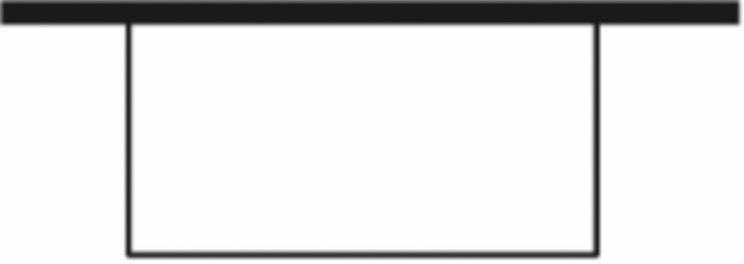
\includegraphics[width=0.28\textwidth]{figures/gao92_q8_fence.png}
\end{center}

\ifanswer
\solbegin
\step{设矩形的长为 $x$ 米，宽为 $y$，则 $xy=18$，}
\step{需要用栅栏长为 $x+2y\geqslant2\sqrt{2xy}=12$，}
\step{当且仅当 $x=2y$，即 $y=3$，$x=6$ 时取等号，故至少需要 $12$ 米栅栏.}
\solend
\fi

\item 已知 $a$ 为正整数，若关于 $x$ 的不等式 $\lvert x-2025\rvert\leqslant a$ 的解集中有且仅有 $7$ 个整数，则 $a$ 的值为\blankline[4.4em].

\ifanswer
\solbegin
\step{不等式 $\lvert x-2025\rvert\leqslant a$，则 $-a\leqslant x-2025\leqslant a$，即 $2025-a\leqslant x\leqslant2025+a$，}
\step{所以不等式 $\lvert x-2025\rvert\leqslant a$ 的解集为 $\{x\mid2025-a\leqslant x\leqslant2025+a\}$，}
\step{若不等式解集中有且仅有 $7$ 个整数，且 $a$ 为正整数，}
\step{由解集的对称性得这 $7$ 个整数以 $2025$ 为中心，向左右两边各延伸 $3$ 个整数，}
\step{即这 $7$ 个整数为 $2022,2023,2024,2025,2026,2027,2028$，所以 $a=3$.}
\solend
\fi

\item 已知关于 $x$ 的一元二次方程 $x^2-x+a=0$ 有两个不相等的正根 $m$、$n$，则 $\dfrac1m+\dfrac9n$ 的最小值为\blankline[4.4em].

\ifanswer
\solbegin
\step{因为一元二次方程 $x^2-x+a=0$ 有两个不相等的正根 $m$、$n$，}
\step{所以判别式 $\Delta=(-1)^2-4a>0\Rightarrow a<\dfrac14$，$m+n=1$，$mn=a>0$，}
\step{因此 $0<a<\dfrac14$ 且 $m+n=1(m,n>0)$.}
\step{$\dfrac1m+\dfrac9n=\left(\dfrac1m+\dfrac9n\right)(m+n)=1+\dfrac nm+\dfrac{9m}{n}+9=10+\dfrac nm+\dfrac{9m}{n}\geqslant10+2\sqrt9=16$，}
\step{等号成立条件为 $\dfrac nm=\dfrac{9m}{n}\Rightarrow n^2=9m^2\Rightarrow n=3m$，}
\step{$m$、$n>0$，结合 $m+n=1$，代入 $n=3m$ 得 $m+3m=1\Rightarrow m=\dfrac14$，$n=\dfrac34$，}
\step{此时 $mn=\dfrac14\cdot\dfrac34=\dfrac3{16}$，满足 $0<a<\dfrac14$，等号可取，因此 $\dfrac1m+\dfrac9n$ 的最小值为 $16$.}
\solend
\fi

\item 对任意 $A$、$B\subseteq R$，记 $A\oplus B=\{x\mid x\in A\cup B,x\notin A\cap B\}$，并称 $A\oplus B$ 为集合 $A$，$B$ 的对称差. 例如：若 $A=\{1,2,3\},B=\{2,3,4\}$，则 $A\oplus B=\{1,4\}$. 下列命题中，为真命题的有\blankline[4.4em].

①若 $A$、$B\subseteq R$ 且 $A\oplus B\subseteq A$，则 $A\subseteq B$

②若 $A$、$B\subseteq R$ 且 $A\oplus B=\varnothing$，则 $A=B$

③若 $A$、$B\subseteq R$ 且 $A\oplus B=B$，则 $A=\varnothing$

④对任意 $A$、$B\subseteq R$，都有 $A\oplus B=\complement_{R}A\oplus\complement_{R}B$

\ifanswer
\solbegin
\step{对于①，因为 $A\oplus B\subseteq A$，所以 $\{x\mid x\in A\cup B,x\notin A\cap B\}\subseteq A$，故 $B\subseteq A$，}
\step{故①错误；}
\step{对于②，$A$、$B\subseteq R$ 且 $A\oplus B=\varnothing$，则 $\varnothing=\{x\mid x\in A\cup B,x\notin A\cap B\}$，}
\step{即 $A\cup B=A\cap B$，所以 $A=B$，故②正确；}
\step{对于③，$A$、$B\subseteq R$ 且 $A\oplus B=B$，则 $B=\{x\mid x\in A\cup B,x\notin A\cap B\}$，}
\step{故 $A\subseteq B$，且 $B$ 中元素不在 $A\cap B$ 中，故 $A=\varnothing$，故③正确；}
\step{对于④，$\complement_{R}A\oplus\complement_{R}B=\{x\mid x\in\complement_{R}A\cup\complement_{R}B,x\notin\complement_{R}A\cap\complement_{R}B\}$，}
\step{其中 $\complement_{R}A\cup\complement_{R}B=\complement_{R}(A\cap B)$，$\complement_{R}A\cap\complement_{R}B=\complement_{R}(A\cup B)$，}
\step{故 $\complement_{R}A\oplus\complement_{R}B=\{x\mid x\in\complement_{R}(A\cap B)$，}
\step{$x\notin\complement_{R}(A\cup B)\}=\{x\mid x\in A\cup B,x\notin A\cap B\}$，}
\step{而 $A\oplus B=\{x\mid x\in A\cup B,x\notin A\cap B\}$，故 $A\oplus B=\complement_{R}A\oplus\complement_{R}B$，故④正确.}
\step{故正确的是②③④.}
\solend
\fi

\item 若不等式 $x^2-2ax+a^2-1\geqslant0$ 对任意 $x\in[0,2]$ 恒成立，则实数 $a$ 的取值范围是\blankline[4.4em].

\ifanswer
\solbegin
\step{由题意不等式 $x^2-2ax+a^2-1\geqslant0$ 对任意 $x\in[0,2]$ 恒成立，}
\step{解得 $x\leqslant a-1$ 或 $x\geqslant a+1$，要使此不等式对任意 $x\in[0,2]$ 恒成立，}
\step{则区间 $[0,2]$ 必须完全包含在解集 $(-\infty,a-1]\cup[a+1,+\infty)$ 中，}
\step{等价于 $[0,2]$ 与开区间 $(a-1,a+1)$ 的交集为空集，}
\step{区间 $[0,2]$ 在 $a-1$ 左侧，即 $2\leqslant a-1$，解得 $a\geqslant3$，}
\step{区间 $[0,2]$ 在 $a+1$ 右侧，即 $a+1\leqslant0$，解得 $a\leqslant-1$，}
\step{当 $a\in(-1,3)$，则 $(a-1,a+1)$ 与 $[0,2]$ 必有交集，不满足条件，}
\step{综上，实数 $a$ 的取值范围是 $(-\infty,-1]\cup[3,+\infty)$.}
\solend
\fi

\end{enumerate}

\bigsec{二、选择题}

\begin{enumerate}
\setcounter{enumi}{12}

\item 若 $a<b<0$，则下列不等式成立的是\mbox{（\quad）}% 原卷括号内已印“D”，试卷版按惯例留空

\keepwithprev
A. $a^2<b^2$\qquad B. $\dfrac1a<\dfrac1b$\qquad C. $ab<b^2$\qquad D. $ab<a^2$

\ifanswer
\ans{$D$}
\fi

\item 已知全集 $U=\{1,2,3,4,5\}$，集合 $A,B$ 是 $U$ 子集，满足 $\overline{A\cup B}=\{4,5\}$，$B=\{2,3\}$，则 $A\cap\overline B=\mbox{（\quad）}$

\keepwithprev
A. $\{1\}$\qquad B. $\{1,2\}$\qquad C. $\{1,4,5\}$\qquad D. $\varnothing$

\ifanswer
\solbegin
\step{因为全集 $U=\{1,2,3,4,5\}$，集合 $A$、$B$ 是 $U$ 子集，$\overline{A\cup B}=\{4,5\}$，$B=\{2,3\}$，}
\step{所以 $A\cup B=\{1,2,3\}$，故 $1\in A$，$1\notin B$，$4\notin A$，$5\notin A$，$4\notin B$，$5\notin B$，}
\step{故 $A\cap\overline B=\{1\}$. 故选 $A$.}
\solend
\fi

\item 设 $a>0$，若关于 $x$ 的不等式 $x^2-(2a-1)x-2a<0$ 的解集中恰有 $3$ 个整数，则实数 $a$ 的取值范围是\mbox{（\quad）}

\keepwithprev
A. $\left[1,\dfrac32\right]$\qquad B. $\left(1,\dfrac32\right]$\qquad C. $\left[\dfrac12,1\right]$\qquad D. $\left(\dfrac12,1\right]$

\ifanswer
\solbegin
\step{已知关于 $x$ 的不等式 $x^2-(2a-1)x-2a<0$，则 $(x+1)(x-2a)<0$，}
\step{则 $-1<x<2a$，又解集中恰有 $3$ 个整数，则 $2<2a\leqslant3$，则 $1<a\leqslant\dfrac32$，}
\step{则 $a$ 的取值范围为 $\left(1,\dfrac32\right]$. 故选 $B$.}
\solend
\fi

\item 已知集合 $U=\{1,2,3,\cdots,2027\}$，$M\subseteq U$，若对于 $M$ 中的任意两个不同的元素 $x$、$y$，都有 $\lvert x-y\rvert>2$，则 $M$ 中元素个数的最大值为\mbox{（\quad）}

\keepwithprev
A. $675$\qquad B. $676$\qquad C. $2025$\qquad D. $2026$

\ifanswer
\solbegin
\step{对于 $M$ 中的任意两个不同的元素 $x$、$y$，都有 $\lvert x-y\rvert>2$，}
\step{不妨设 $x>y$，都有 $x-y\geqslant3$，}
\step{要想 $M$ 所含元素个数最大，则要 $x-y$ 尽可能小，故需使得 $x-y$ 的最小值为 $3$，}
\step{将 $1\sim2027$ 这 $2027$ 个元素按如下分组：}
\step{$\{1,2,3\},\{4,5,6\},\cdots,\{2023,2024,2025\},\{2026,2027\}$，}
\step{故应在前 $675$ 组中按周期 $3$ 每组取一个元素，且第一组中不能取 $3$，}
\step{第一组中取 $1$ 时，得 $M=\{1,4,7,\cdots,2023,2026\}$}
\step{或 $M=\{1,4,7,\cdots,2023,2027\}$ 这样的集合，}
\step{第一组取 $2$ 时，得 $M=\{2,5,8,\cdots,2024,2027\}$，}
\step{其中任意两元素差值 $x-y(x>y)$ 都大于 $2$，满足题意，}
\step{故 $M$ 所含元素个数的最大值为 $\dfrac{2025}{3}+1=676$. 故选 $B$.}
\solend
\fi

\end{enumerate}

\bigsec{三、解答题}

\begin{enumerate}
\setcounter{enumi}{16}

\item 已知集合 $M=\{x\mid a-1\leqslant x\leqslant2a+3\}$，$P=\{x\mid-2<x\leqslant4\}$，全集 $U=R$.

（1）当 $a=2$ 时，求 $M\cap P$；

（2）若 $x\in P$ 是 $x\in M$ 的必要不充分条件，求实数 $a$ 的取值范围.

\ansspace*[9]

\ifanswer
\solbegin
\stepm{（1）}{当 $a=2$ 时，集合 $M=\{x\mid1\leqslant x\leqslant7\}$，所以 $M\cap P=\{x\mid1\leqslant x\leqslant4\}$；}
\stepm{（2）}{因为 $x\in P$ 是 $x\in M$ 的必要不充分条件，所以 $M\subsetneqq P$，}
\step{当 $M=\varnothing$ 时，$a-1>2a+3$，解得 $a<-4$，}
\step{当 $M\neq\varnothing$ 时，则 $\begin{cases}a-1\leqslant2a+3\\ a-1>-2\\ 2a+3\leqslant4\end{cases}$，解得 $-1<a\leqslant\dfrac12$，}
\step{综上所述，实数 $a$ 的取值范围为 $(-\infty,-4)\cup\left(-1,\dfrac12\right]$.}
\solend
\fi

\item 命题甲：关于 $x$ 的方程 $(a-1)x^2+(2a-4)x+a=0$ 有两个不相等的实数根；

命题乙：关于 $x$ 的不等式 $ax^2-2ax+a+1>0$ 的解集为 $R$.

（1）若命题甲为真命题，求实数 $a$ 的取值范围；

（2）若命题甲、乙中至多有一个为真命题，求实数 $a$ 的取值范围.

\ansspace*[12]

\ifanswer
\solbegin
\stepm{（1）}{命题甲：关于 $x$ 的方程 $(a-1)x^2+(2a-4)x+a=0$ 有两个不相等的实数根，}
\step{则 $\begin{cases}a-1\neq0\\ \Delta=(2a-4)^2-4a(a-1)>0\end{cases}$，解得 $a<\dfrac43$ 且 $a\neq1$，}
\step{故 $a$ 的范围为 $\left\{a\left|a<\dfrac43\ \text{且}\ a\neq1\right.\right\}$；}
\stepm{（2）}{当 $a=0$ 时 $y=1>0$，符合题意；}
\step{当 $a\neq0$，由 $\begin{cases}a>0\\ \Delta=4a^2-4a(a+1)<0\end{cases}$，解得 $a>0$，}
\step{则 $a$ 的取值范围为 $a\geqslant0$，}
\step{故 $p$、$q$ 都为真时，$a$ 的范围为 $0\leqslant a<\dfrac43$ 且 $a\neq1$，}
\step{则命题甲、乙中至多有一个为真命题时，}
\step{$a$ 的取值范围为 $\left\{a\left|a<0\ \text{或}\ a=1\ \text{或}\ a\geqslant\dfrac43\right.\right\}$.}
\solend
\fi

\item 如图，$OA$、$OB$ 是两条长度足够长的互相垂直的笔直小路，矩形 $OCPD$ 的顶点 $C$，$D$ 分别在 $OA$、$OB$ 上，且该矩形区域内种满了荷花. 为了让观赏者有更好的观赏体验，现计划经过点 $P$ 修一条小路 $EF$，其中点 $E$ 在小路 $OA$ 上，点 $F$ 在小路 $OB$ 上，并在 $\triangle OEF$ 区域内种满荷花. 已知 $OD=25$ m，$OC=40$ m，且小路 $EF$ 要完全位于一个以 $O$ 为顶点的，边长为 $100$ m 的正方形内部（包括边界）. 记 $\triangle OEF$ 的面积为 $S$ m$^2$.

\begin{center}
\begin{tikzpicture}[x=0.46cm,y=0.42cm,line width=0.7pt]
\draw (0,0) -- (0,10.2) node[above,inner sep=3pt] {$A$};
\draw (0,0) -- (11.8,0) node[right,inner sep=3pt] {$B$};
\draw (0,4.83) -- (2.42,4.83) -- (2.42,0);
\draw (0,6.92) -- (8.01,0);
\node[below left,inner sep=2pt] at (0,0) {$O$};
\node[below,inner sep=2pt] at (2.42,0) {$D$};
\node[left,inner sep=3pt] at (0,4.83) {$C$};
\node[above right,inner sep=1pt] at (2.42,4.83) {$P$};
\node[left,inner sep=3pt] at (0,6.92) {$E$};
\node[below,inner sep=2pt] at (8.01,0) {$F$};
\end{tikzpicture}
\end{center}

（1）设 $EC=x\cdot m$，试用 $x$ 表示 $OF$，并求 $x$ 的取值范围.

（2）当 $EC$ 的长度为多少时，$S$ 取得最小值？最小值是多少？

\ansspace*[11]

\ifanswer
\solbegin
\stepm{（1）}{由题意得 $x\leqslant60$，}
\step{$\triangle PCE\backsim\triangle FDP$，所以 $\dfrac{EC}{CP}=\dfrac{PD}{DF}$，即 $\dfrac{x}{25}=\dfrac{40}{DF}$，得 $DF=\dfrac{1000}{x}$ m，}
\step{所以 $OF=OD+DF=\left(25+\dfrac{1000}{x}\right)$ m，}
\step{所以 $25+\dfrac{1000}{x}\leqslant100$，解得 $x\geqslant\dfrac{40}{3}$；}
\step{综上，$\dfrac{40}{3}\leqslant x\leqslant60$；}
\stepm{（2）}{由 $OE=OC+CE=(40+x)$ m，}
\step{所以 $S=\dfrac12\cdot OF\cdot OE=\dfrac12\left(25+\dfrac{1000}{x}\right)(40+x)$}
\step{$=\dfrac12\left(1000+25x+\dfrac{40000}{x}+1000\right)$ m$^2$，}
\step{由基本不等式得 $S\geqslant\dfrac12\left(2000+2\sqrt{25x\cdot\dfrac{40000}{x}}\right)=2000$ m$^2$，}
\step{当且仅当 $25x=\dfrac{40000}{x}$，即 $x=40$ 时取等号，}
\step{故 $EC=40$ m 时，$S$ 取得最小值，为 $2000$ m$^2$.}
\solend
\fi

\item 已知函数 $f(x)=x^2-(a-2)x+a-3$.

（1）若 $f(x)=0$ 的两根为 $\alpha,\beta$，$\alpha^2+\beta^2=2$，求 $a$ 的值；

（2）解关于 $x$ 的不等式 $f(x)\geqslant0$；

（3）是否存在整数 $m,n$，使得关于 $x$ 的不等式 $m\leqslant f(x)\leqslant n$ 的解集恰好为 $[m,n]$？若存在，求出 $m,n$ 的值. 若不存在，请说明理由.

\ansspace*[16]

\ifanswer
\solbegin
\stepm{（1）}{由韦达定理，$\alpha+\beta=a-2,\alpha\beta=a-3$，}
\step{因此 $\alpha^2+\beta^2=(a-2)^2-2(a-3)=2\Leftrightarrow(a-2)(a-4)=0$，}
\step{$a=2$ 时两根为 $1,-1$；$a=4$ 时两根均为 $1$，均满足条件，}
\step{所以 $a=2$ 或 $a=4$.}
\stepm{（2）}{因为 $f(x)=(x-1)[x-(a-3)]$，所以分三种情况：}
\step{当 $a<4$ 时，$a-3<1$，解集为 $(-\infty,a-3]\cup[1,+\infty)$.}
\step{当 $a=4$ 时，$f(x)=(x-1)^2\geqslant0$ 恒成立，解集为 $R$.}
\step{当 $a>4$ 时，$a-3>1$，解集为 $(-\infty,1]\cup[a-3,+\infty)$.}
\stepm{（3）}{区间 $[m,n]$ 要求 $m<n$. 记 $f(x)$ 的最小值为 $k$.}
\step{$[m,n]$ 非空，不等式 $f(x)\leqslant n$ 有解，其解集为闭区间 $[x_1,x_2]$，}
\step{其中 $x_1\leqslant x_2$ 是方程 $f(x)=n$ 的两根.}
\step{若 $k<m$，则 $f(x)<m$ 的解集是 $[x_1,x_2]$ 内部的一个开区间，}
\step{从 $[x_1,x_2]$ 中去掉它后剩下两段，原不等式的解集不是一个区间，矛盾，}
\step{所以 $k\geqslant m$，原不等式的解集就是 $[x_1,x_2]$，于是 $m=x_1,n=x_2$，}
\step{即 $f(m)=f(n)=n$，于是 $f(m)-f(n)=(m-n)(m+n-a+2)=0$.}
\step{因为 $m\neq n$，所以 $a=m+n+2$.}
\step{代入 $f(m)=n$，得 $(m-1)(1-n)=n\Leftrightarrow m(n-1)=-1$，$m,n$ 均为整数，}
\step{因此 $(m,n)=(-1,2)$ 或 $(m,n)=(1,0)$.}
\step{结合 $m<n$，只可能有 $m=-1,n=2$，此时 $a=3$.}
\step{检验：此时 $f(x)=x^2-x$，且 $x^2-x=\left(x-\dfrac12\right)^2-\dfrac14\geqslant-\dfrac14>-1$，}
\step{因此 $-1\leqslant f(x)\leqslant2\Leftrightarrow x^2-x\leqslant2\Leftrightarrow(x+1)(x-2)\leqslant0\Leftrightarrow x\in[-1,2]$，}
\step{所以存在符合条件的整数 $m=-1,n=2$.}
\solend
\fi

\item 给定数集 $M$，若对于任意 $a$、$b\in M$，有 $a+b\in M,a-b\in M$，则称集合 $M$ 为闭集合.

（1）判断集合 $A_1=\{-4,-2,0,2,4\}$，集合 $B=\{x\mid x=3k,k\in\Z\}$ 是否为闭集合；

（2）若集合 $C$、$D$ 为闭集合，则 $C\cup D$ 是否一定为闭集合？请说明理由；

（3）已知集合 $C$、$D$ 为闭集合，且 $C\subsetneq R,D\subsetneq R$，证明：$(C\cup D)\subsetneq R$.% 原卷印作 (C∪D)⊂R，按解析证明的是 C∪D≠R，排真子集

\ansspace*[14]

\ifanswer
\solbegin
\stepm{（1）}{因为 $4\in A_1$，$2\in A_1$，$4+2=6\notin A_1$，所以 $A_1$ 不是闭集合；}
\step{任取 $x,y\in B$，设 $x=3m,y=3n,m,n\in\Z$，}
\step{则 $x+y=3m+3n=3(m+n)$ 且 $m+n\in\Z$，}
\step{所以 $x+y\in B$，同理，$x-y\in B$，故 $B$ 为闭集合.}
\stepm{（2）}{结论：不一定.}
\step{不妨令 $C=\{x\mid x=2k,k\in\Z\},D=\{x\mid x=3k,k\in\Z\}$，}
\step{则由（1）得 $C$、$D$ 为闭集合，易得 $2,3\in C\cup D,2+3=5\notin C\cup D$，}
\step{因此，$C\cup D$ 不一定是闭集合.}
\stepm{（3）}{不妨假设 $C\cup D=R$，则由 $C\subsetneq R$，得存在 $a\in R$ 且 $a\notin C$，故 $a\in D$.}
\step{同理，存在 $b\in R$ 且 $b\notin D$，故 $b\in C$.}
\step{因为 $a+b\in R=C\cup D$，所以 $a+b\in C$ 或 $a+b\in D$.}
\step{若 $a+b\in C$，则由 $C$ 为闭集合且 $b\in C$，得 $a=(a+b)-b\in C$，}
\step{与 $a\notin C$ 矛盾.}
\step{若 $a+b\in D$，则由 $D$ 为闭集合且 $a\in D$，得 $b=(a+b)-a\in D$，}
\step{与 $b\notin D$ 矛盾.}
\step{综上，$C\cup D=R$ 不成立，故 $(C\cup D)\subsetneq R$.}
\solend
\fi

\end{enumerate}

\end{document}
"
%
% 原始材料：微信公众号“魔都数学加油站”文章，连载“27学年高一92”；
% 原文标题“27学年高一92——2026-2027年上海市闵行实验高一上10月月考”；
% 原文链接：https://mp.weixin.qq.com/s/8HUyr3G7GpcHyczwu_XYCQ。
% 正文为 10 张 PNG 页（`原图/高一92_闵行实验_10月月考/01..10.png`），均 4762×6735，按页序读取。
%
% 篇幅与题号：原卷自第 3 题起编号（第 1、2 题不在原文内）。填空题 3—12（10 题）、
% 选择题 13—16（4 题）、解答题 17—21（5 题），共 19 题。
%
% 讲评版：第 6 题只印【答案】（“$[-1,3]$”），本稿只给 \ans{}；第 13 题无【解析】、
% 答案“D”直接印在题干括号内，本稿试卷版按惯例留空、答案版提 \ans{$D$}；其余 17 题印
% 【解析】，其中选择题答案在解析末句“故选 $A$／$B$／$B$”。
% 第 8 题题干右侧有一幅“围墙 + 三面栅栏”示意图（裁自第 2 页原图）；第 19 题题干带
% 与 高一88 第 19 题同型的示意图（$OA$／$OB$ 两条小路、矩形 $OCPD$、折线 $EF$），用 TikZ 重绘。
%
% 副标题：原卷未印副标题。本稿按内容标作“集合与常用逻辑用语、不等式”。
%
% 原卷笔误/存疑（均照录未改，正文对应处另有 % 注）：
%   ① 第 21 题 (3) 题干与解析末句把结论印作“$(C\cup D)\subset R$”，而解析证明的是
%      “$C\cup D=\R$ 不成立”，按文意应为“$(C\cup D)\subsetneq\R$”；本稿按真子集排
%      $\subsetneq$，原卷记号照录于文件头；
%   ② 第 7 题解析只列 $B=\varnothing$（$a=0$）、$B=\{1\}$（$a=1$）、$B=\{-3\}$（$a=-\frac13$）
%      三种情形，与结论 $\left\{0,1,-\frac13\right\}$ 相符，无笔误。
%
% 与原卷的排版差异：
%   ① 原卷每题下直接印【答案】/【解析】，本稿按全稿惯例将答案与解析置于答案版；
%   ② 原卷未印副标题，本稿补出；填空横线统一排 \blankline[4.4em]；
%   ③ 原卷数集记号排斜体 $R$、$Z$，本稿按全稿惯例改用 $\R$、$\Z$；
%   ④ 第 17—21 题的子问用行内“（1）（2）（3）”段，解析中的子问标号用 \stepm；
%   ⑤ 解答题按惯例加 \ansspace；选择题括号排 \mbox{（\quad）}；
%   ⑥ 第 8 题的示意图原卷排在题干右侧、文字绕排，本稿改排为题干后的居中图
%      （自原图裁切、去粉色水印后转灰度）；第 19 题的图按原图比例 TikZ 重绘。
%
% 行数核对：逐题数 \step/\stepm 条数，合计 128 条（Q3：2；Q4：3；Q5：2；Q6：0；Q7：6；
% Q8：3；Q9：5；Q10：7；Q11：12；Q12：8；Q13：0；Q14：3；Q15：3；Q16：11；Q17：5；
% Q18：9；Q19：11；Q20：22；Q21：16）。第 6 题只印答案、第 13 题无解析，均不计入 \step 账。
% 原卷解析的换行按语意合并，未逐行强拆。
%
\documentclass[a4paper,11pt]{article}
\usepackage{common}

\begin{document}

\examtitlest[7]{2026--2027 年闵行实验高一上 10 月月考}{集合与常用逻辑用语、不等式}

\bigsec{一、填空题}

\begin{enumerate}
\setcounter{enumi}{2}

\item 已知 $3<a<8$，$4<b<9$，则 $\dfrac ab$ 的取值范围是\blankline[4.4em].

\ifanswer
\solbegin
\step{因为 $4<b<9$，所以 $\dfrac19<\dfrac1b<\dfrac14$，又 $3<a<8$，所以 $\dfrac13<\dfrac ab<2$，}
\step{故 $\dfrac ab$ 的取值范围是 $\left(\dfrac13,2\right)$.}
\solend
\fi

\item 已知 $p:x>3$，$q:x>5$，则 $p$ 是 $q$ 的\blankline[4.4em]（选“充分不必要条件”“必要不充分条件”“充要条件”“既不充分也不必要条件”之一填空）.

\ifanswer
\solbegin
\step{当 $x>3$ 时，不能推出 $x>5$，充分性不成立；}
\step{当 $x>5$ 时，可以得到 $x>3$，必要性成立；}
\step{故 $p$ 是 $q$ 的必要不充分条件.}
\solend
\fi

\item 不等式 $\dfrac{x-1}{2x+1}\leqslant1$ 的解集为\blankline[4.4em].

\ifanswer
\solbegin
\step{因为 $\dfrac{x-1}{2x+1}\leqslant1$，所以 $\dfrac{x-1}{2x+1}-\dfrac{2x+1}{2x+1}\leqslant0$，所以 $\dfrac{x+2}{2x+1}\geqslant0$，}
\step{所以 $x>-\dfrac12$ 或 $x\leqslant-2$，即不等式的解集是 $(-\infty,-2]\cup\left(-\dfrac12,+\infty\right)$.}
\solend
\fi

\item 设 $x\in R$，则方程 $\lvert x+1\rvert+\lvert x-3\rvert=4$ 的解集为\blankline[4.4em].

\ifanswer
\ans{$[-1,3]$}
\fi

\item 若 $A=\{x\mid x^2+2x=3\}$，$B=\{x\mid ax=1\}$，且 $B\subseteq A$，则实数 $a$ 的值组成的集合为\blankline[4.4em].

\ifanswer
\solbegin
\step{由 $x^2+2x=3$ 得 $x^2+2x-3=0$，解得 $x=1$ 或 $x=-3$，所以 $A=\{1,-3\}$，}
\step{又因为 $B=\{x\mid ax=1\}$，且 $B\subseteq A$，}
\step{当 $B=\varnothing$，即 $a=0$ 时，显然符合题意；}
\step{当 $B=\{1\}$，即 $a=1$ 时，也符合题意；}
\step{当 $B=\{-3\}$，即 $a=-\dfrac13$ 时，也符合题意；}
\step{综上所述，实数 $a$ 的值组成的集合为 $\left\{0,1,-\dfrac13\right\}$.}
\solend
\fi

\item 某校欲在围墙边用栅栏围成一个 $18$ 平方米的矩形区域，作为天鹅的地面栖息地，矩形区域的一条边为围墙（如图），则至少需要\blankline[4.4em]米栅栏.

\begin{center}
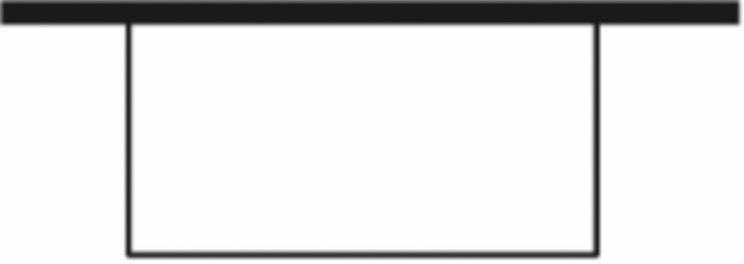
\includegraphics[width=0.28\textwidth]{figures/gao92_q8_fence.png}
\end{center}

\ifanswer
\solbegin
\step{设矩形的长为 $x$ 米，宽为 $y$，则 $xy=18$，}
\step{需要用栅栏长为 $x+2y\geqslant2\sqrt{2xy}=12$，}
\step{当且仅当 $x=2y$，即 $y=3$，$x=6$ 时取等号，故至少需要 $12$ 米栅栏.}
\solend
\fi

\item 已知 $a$ 为正整数，若关于 $x$ 的不等式 $\lvert x-2025\rvert\leqslant a$ 的解集中有且仅有 $7$ 个整数，则 $a$ 的值为\blankline[4.4em].

\ifanswer
\solbegin
\step{不等式 $\lvert x-2025\rvert\leqslant a$，则 $-a\leqslant x-2025\leqslant a$，即 $2025-a\leqslant x\leqslant2025+a$，}
\step{所以不等式 $\lvert x-2025\rvert\leqslant a$ 的解集为 $\{x\mid2025-a\leqslant x\leqslant2025+a\}$，}
\step{若不等式解集中有且仅有 $7$ 个整数，且 $a$ 为正整数，}
\step{由解集的对称性得这 $7$ 个整数以 $2025$ 为中心，向左右两边各延伸 $3$ 个整数，}
\step{即这 $7$ 个整数为 $2022,2023,2024,2025,2026,2027,2028$，所以 $a=3$.}
\solend
\fi

\item 已知关于 $x$ 的一元二次方程 $x^2-x+a=0$ 有两个不相等的正根 $m$、$n$，则 $\dfrac1m+\dfrac9n$ 的最小值为\blankline[4.4em].

\ifanswer
\solbegin
\step{因为一元二次方程 $x^2-x+a=0$ 有两个不相等的正根 $m$、$n$，}
\step{所以判别式 $\Delta=(-1)^2-4a>0\Rightarrow a<\dfrac14$，$m+n=1$，$mn=a>0$，}
\step{因此 $0<a<\dfrac14$ 且 $m+n=1(m,n>0)$.}
\step{$\dfrac1m+\dfrac9n=\left(\dfrac1m+\dfrac9n\right)(m+n)=1+\dfrac nm+\dfrac{9m}{n}+9=10+\dfrac nm+\dfrac{9m}{n}\geqslant10+2\sqrt9=16$，}
\step{等号成立条件为 $\dfrac nm=\dfrac{9m}{n}\Rightarrow n^2=9m^2\Rightarrow n=3m$，}
\step{$m$、$n>0$，结合 $m+n=1$，代入 $n=3m$ 得 $m+3m=1\Rightarrow m=\dfrac14$，$n=\dfrac34$，}
\step{此时 $mn=\dfrac14\cdot\dfrac34=\dfrac3{16}$，满足 $0<a<\dfrac14$，等号可取，因此 $\dfrac1m+\dfrac9n$ 的最小值为 $16$.}
\solend
\fi

\item 对任意 $A$、$B\subseteq R$，记 $A\oplus B=\{x\mid x\in A\cup B,x\notin A\cap B\}$，并称 $A\oplus B$ 为集合 $A$，$B$ 的对称差. 例如：若 $A=\{1,2,3\},B=\{2,3,4\}$，则 $A\oplus B=\{1,4\}$. 下列命题中，为真命题的有\blankline[4.4em].

①若 $A$、$B\subseteq R$ 且 $A\oplus B\subseteq A$，则 $A\subseteq B$

②若 $A$、$B\subseteq R$ 且 $A\oplus B=\varnothing$，则 $A=B$

③若 $A$、$B\subseteq R$ 且 $A\oplus B=B$，则 $A=\varnothing$

④对任意 $A$、$B\subseteq R$，都有 $A\oplus B=\complement_{R}A\oplus\complement_{R}B$

\ifanswer
\solbegin
\step{对于①，因为 $A\oplus B\subseteq A$，所以 $\{x\mid x\in A\cup B,x\notin A\cap B\}\subseteq A$，故 $B\subseteq A$，}
\step{故①错误；}
\step{对于②，$A$、$B\subseteq R$ 且 $A\oplus B=\varnothing$，则 $\varnothing=\{x\mid x\in A\cup B,x\notin A\cap B\}$，}
\step{即 $A\cup B=A\cap B$，所以 $A=B$，故②正确；}
\step{对于③，$A$、$B\subseteq R$ 且 $A\oplus B=B$，则 $B=\{x\mid x\in A\cup B,x\notin A\cap B\}$，}
\step{故 $A\subseteq B$，且 $B$ 中元素不在 $A\cap B$ 中，故 $A=\varnothing$，故③正确；}
\step{对于④，$\complement_{R}A\oplus\complement_{R}B=\{x\mid x\in\complement_{R}A\cup\complement_{R}B,x\notin\complement_{R}A\cap\complement_{R}B\}$，}
\step{其中 $\complement_{R}A\cup\complement_{R}B=\complement_{R}(A\cap B)$，$\complement_{R}A\cap\complement_{R}B=\complement_{R}(A\cup B)$，}
\step{故 $\complement_{R}A\oplus\complement_{R}B=\{x\mid x\in\complement_{R}(A\cap B)$，}
\step{$x\notin\complement_{R}(A\cup B)\}=\{x\mid x\in A\cup B,x\notin A\cap B\}$，}
\step{而 $A\oplus B=\{x\mid x\in A\cup B,x\notin A\cap B\}$，故 $A\oplus B=\complement_{R}A\oplus\complement_{R}B$，故④正确.}
\step{故正确的是②③④.}
\solend
\fi

\item 若不等式 $x^2-2ax+a^2-1\geqslant0$ 对任意 $x\in[0,2]$ 恒成立，则实数 $a$ 的取值范围是\blankline[4.4em].

\ifanswer
\solbegin
\step{由题意不等式 $x^2-2ax+a^2-1\geqslant0$ 对任意 $x\in[0,2]$ 恒成立，}
\step{解得 $x\leqslant a-1$ 或 $x\geqslant a+1$，要使此不等式对任意 $x\in[0,2]$ 恒成立，}
\step{则区间 $[0,2]$ 必须完全包含在解集 $(-\infty,a-1]\cup[a+1,+\infty)$ 中，}
\step{等价于 $[0,2]$ 与开区间 $(a-1,a+1)$ 的交集为空集，}
\step{区间 $[0,2]$ 在 $a-1$ 左侧，即 $2\leqslant a-1$，解得 $a\geqslant3$，}
\step{区间 $[0,2]$ 在 $a+1$ 右侧，即 $a+1\leqslant0$，解得 $a\leqslant-1$，}
\step{当 $a\in(-1,3)$，则 $(a-1,a+1)$ 与 $[0,2]$ 必有交集，不满足条件，}
\step{综上，实数 $a$ 的取值范围是 $(-\infty,-1]\cup[3,+\infty)$.}
\solend
\fi

\end{enumerate}

\bigsec{二、选择题}

\begin{enumerate}
\setcounter{enumi}{12}

\item 若 $a<b<0$，则下列不等式成立的是\mbox{（\quad）}% 原卷括号内已印“D”，试卷版按惯例留空

\keepwithprev
A. $a^2<b^2$\qquad B. $\dfrac1a<\dfrac1b$\qquad C. $ab<b^2$\qquad D. $ab<a^2$

\ifanswer
\ans{$D$}
\fi

\item 已知全集 $U=\{1,2,3,4,5\}$，集合 $A,B$ 是 $U$ 子集，满足 $\overline{A\cup B}=\{4,5\}$，$B=\{2,3\}$，则 $A\cap\overline B=\mbox{（\quad）}$

\keepwithprev
A. $\{1\}$\qquad B. $\{1,2\}$\qquad C. $\{1,4,5\}$\qquad D. $\varnothing$

\ifanswer
\solbegin
\step{因为全集 $U=\{1,2,3,4,5\}$，集合 $A$、$B$ 是 $U$ 子集，$\overline{A\cup B}=\{4,5\}$，$B=\{2,3\}$，}
\step{所以 $A\cup B=\{1,2,3\}$，故 $1\in A$，$1\notin B$，$4\notin A$，$5\notin A$，$4\notin B$，$5\notin B$，}
\step{故 $A\cap\overline B=\{1\}$. 故选 $A$.}
\solend
\fi

\item 设 $a>0$，若关于 $x$ 的不等式 $x^2-(2a-1)x-2a<0$ 的解集中恰有 $3$ 个整数，则实数 $a$ 的取值范围是\mbox{（\quad）}

\keepwithprev
A. $\left[1,\dfrac32\right]$\qquad B. $\left(1,\dfrac32\right]$\qquad C. $\left[\dfrac12,1\right]$\qquad D. $\left(\dfrac12,1\right]$

\ifanswer
\solbegin
\step{已知关于 $x$ 的不等式 $x^2-(2a-1)x-2a<0$，则 $(x+1)(x-2a)<0$，}
\step{则 $-1<x<2a$，又解集中恰有 $3$ 个整数，则 $2<2a\leqslant3$，则 $1<a\leqslant\dfrac32$，}
\step{则 $a$ 的取值范围为 $\left(1,\dfrac32\right]$. 故选 $B$.}
\solend
\fi

\item 已知集合 $U=\{1,2,3,\cdots,2027\}$，$M\subseteq U$，若对于 $M$ 中的任意两个不同的元素 $x$、$y$，都有 $\lvert x-y\rvert>2$，则 $M$ 中元素个数的最大值为\mbox{（\quad）}

\keepwithprev
A. $675$\qquad B. $676$\qquad C. $2025$\qquad D. $2026$

\ifanswer
\solbegin
\step{对于 $M$ 中的任意两个不同的元素 $x$、$y$，都有 $\lvert x-y\rvert>2$，}
\step{不妨设 $x>y$，都有 $x-y\geqslant3$，}
\step{要想 $M$ 所含元素个数最大，则要 $x-y$ 尽可能小，故需使得 $x-y$ 的最小值为 $3$，}
\step{将 $1\sim2027$ 这 $2027$ 个元素按如下分组：}
\step{$\{1,2,3\},\{4,5,6\},\cdots,\{2023,2024,2025\},\{2026,2027\}$，}
\step{故应在前 $675$ 组中按周期 $3$ 每组取一个元素，且第一组中不能取 $3$，}
\step{第一组中取 $1$ 时，得 $M=\{1,4,7,\cdots,2023,2026\}$}
\step{或 $M=\{1,4,7,\cdots,2023,2027\}$ 这样的集合，}
\step{第一组取 $2$ 时，得 $M=\{2,5,8,\cdots,2024,2027\}$，}
\step{其中任意两元素差值 $x-y(x>y)$ 都大于 $2$，满足题意，}
\step{故 $M$ 所含元素个数的最大值为 $\dfrac{2025}{3}+1=676$. 故选 $B$.}
\solend
\fi

\end{enumerate}

\bigsec{三、解答题}

\begin{enumerate}
\setcounter{enumi}{16}

\item 已知集合 $M=\{x\mid a-1\leqslant x\leqslant2a+3\}$，$P=\{x\mid-2<x\leqslant4\}$，全集 $U=R$.

（1）当 $a=2$ 时，求 $M\cap P$；

（2）若 $x\in P$ 是 $x\in M$ 的必要不充分条件，求实数 $a$ 的取值范围.

\ansspace*[9]

\ifanswer
\solbegin
\stepm{（1）}{当 $a=2$ 时，集合 $M=\{x\mid1\leqslant x\leqslant7\}$，所以 $M\cap P=\{x\mid1\leqslant x\leqslant4\}$；}
\stepm{（2）}{因为 $x\in P$ 是 $x\in M$ 的必要不充分条件，所以 $M\subsetneqq P$，}
\step{当 $M=\varnothing$ 时，$a-1>2a+3$，解得 $a<-4$，}
\step{当 $M\neq\varnothing$ 时，则 $\begin{cases}a-1\leqslant2a+3\\ a-1>-2\\ 2a+3\leqslant4\end{cases}$，解得 $-1<a\leqslant\dfrac12$，}
\step{综上所述，实数 $a$ 的取值范围为 $(-\infty,-4)\cup\left(-1,\dfrac12\right]$.}
\solend
\fi

\item 命题甲：关于 $x$ 的方程 $(a-1)x^2+(2a-4)x+a=0$ 有两个不相等的实数根；

命题乙：关于 $x$ 的不等式 $ax^2-2ax+a+1>0$ 的解集为 $R$.

（1）若命题甲为真命题，求实数 $a$ 的取值范围；

（2）若命题甲、乙中至多有一个为真命题，求实数 $a$ 的取值范围.

\ansspace*[12]

\ifanswer
\solbegin
\stepm{（1）}{命题甲：关于 $x$ 的方程 $(a-1)x^2+(2a-4)x+a=0$ 有两个不相等的实数根，}
\step{则 $\begin{cases}a-1\neq0\\ \Delta=(2a-4)^2-4a(a-1)>0\end{cases}$，解得 $a<\dfrac43$ 且 $a\neq1$，}
\step{故 $a$ 的范围为 $\left\{a\left|a<\dfrac43\ \text{且}\ a\neq1\right.\right\}$；}
\stepm{（2）}{当 $a=0$ 时 $y=1>0$，符合题意；}
\step{当 $a\neq0$，由 $\begin{cases}a>0\\ \Delta=4a^2-4a(a+1)<0\end{cases}$，解得 $a>0$，}
\step{则 $a$ 的取值范围为 $a\geqslant0$，}
\step{故 $p$、$q$ 都为真时，$a$ 的范围为 $0\leqslant a<\dfrac43$ 且 $a\neq1$，}
\step{则命题甲、乙中至多有一个为真命题时，}
\step{$a$ 的取值范围为 $\left\{a\left|a<0\ \text{或}\ a=1\ \text{或}\ a\geqslant\dfrac43\right.\right\}$.}
\solend
\fi

\item 如图，$OA$、$OB$ 是两条长度足够长的互相垂直的笔直小路，矩形 $OCPD$ 的顶点 $C$，$D$ 分别在 $OA$、$OB$ 上，且该矩形区域内种满了荷花. 为了让观赏者有更好的观赏体验，现计划经过点 $P$ 修一条小路 $EF$，其中点 $E$ 在小路 $OA$ 上，点 $F$ 在小路 $OB$ 上，并在 $\triangle OEF$ 区域内种满荷花. 已知 $OD=25$ m，$OC=40$ m，且小路 $EF$ 要完全位于一个以 $O$ 为顶点的，边长为 $100$ m 的正方形内部（包括边界）. 记 $\triangle OEF$ 的面积为 $S$ m$^2$.

\begin{center}
\begin{tikzpicture}[x=0.46cm,y=0.42cm,line width=0.7pt]
\draw (0,0) -- (0,10.2) node[above,inner sep=3pt] {$A$};
\draw (0,0) -- (11.8,0) node[right,inner sep=3pt] {$B$};
\draw (0,4.83) -- (2.42,4.83) -- (2.42,0);
\draw (0,6.92) -- (8.01,0);
\node[below left,inner sep=2pt] at (0,0) {$O$};
\node[below,inner sep=2pt] at (2.42,0) {$D$};
\node[left,inner sep=3pt] at (0,4.83) {$C$};
\node[above right,inner sep=1pt] at (2.42,4.83) {$P$};
\node[left,inner sep=3pt] at (0,6.92) {$E$};
\node[below,inner sep=2pt] at (8.01,0) {$F$};
\end{tikzpicture}
\end{center}

（1）设 $EC=x\cdot m$，试用 $x$ 表示 $OF$，并求 $x$ 的取值范围.

（2）当 $EC$ 的长度为多少时，$S$ 取得最小值？最小值是多少？

\ansspace*[11]

\ifanswer
\solbegin
\stepm{（1）}{由题意得 $x\leqslant60$，}
\step{$\triangle PCE\backsim\triangle FDP$，所以 $\dfrac{EC}{CP}=\dfrac{PD}{DF}$，即 $\dfrac{x}{25}=\dfrac{40}{DF}$，得 $DF=\dfrac{1000}{x}$ m，}
\step{所以 $OF=OD+DF=\left(25+\dfrac{1000}{x}\right)$ m，}
\step{所以 $25+\dfrac{1000}{x}\leqslant100$，解得 $x\geqslant\dfrac{40}{3}$；}
\step{综上，$\dfrac{40}{3}\leqslant x\leqslant60$；}
\stepm{（2）}{由 $OE=OC+CE=(40+x)$ m，}
\step{所以 $S=\dfrac12\cdot OF\cdot OE=\dfrac12\left(25+\dfrac{1000}{x}\right)(40+x)$}
\step{$=\dfrac12\left(1000+25x+\dfrac{40000}{x}+1000\right)$ m$^2$，}
\step{由基本不等式得 $S\geqslant\dfrac12\left(2000+2\sqrt{25x\cdot\dfrac{40000}{x}}\right)=2000$ m$^2$，}
\step{当且仅当 $25x=\dfrac{40000}{x}$，即 $x=40$ 时取等号，}
\step{故 $EC=40$ m 时，$S$ 取得最小值，为 $2000$ m$^2$.}
\solend
\fi

\item 已知函数 $f(x)=x^2-(a-2)x+a-3$.

（1）若 $f(x)=0$ 的两根为 $\alpha,\beta$，$\alpha^2+\beta^2=2$，求 $a$ 的值；

（2）解关于 $x$ 的不等式 $f(x)\geqslant0$；

（3）是否存在整数 $m,n$，使得关于 $x$ 的不等式 $m\leqslant f(x)\leqslant n$ 的解集恰好为 $[m,n]$？若存在，求出 $m,n$ 的值. 若不存在，请说明理由.

\ansspace*[16]

\ifanswer
\solbegin
\stepm{（1）}{由韦达定理，$\alpha+\beta=a-2,\alpha\beta=a-3$，}
\step{因此 $\alpha^2+\beta^2=(a-2)^2-2(a-3)=2\Leftrightarrow(a-2)(a-4)=0$，}
\step{$a=2$ 时两根为 $1,-1$；$a=4$ 时两根均为 $1$，均满足条件，}
\step{所以 $a=2$ 或 $a=4$.}
\stepm{（2）}{因为 $f(x)=(x-1)[x-(a-3)]$，所以分三种情况：}
\step{当 $a<4$ 时，$a-3<1$，解集为 $(-\infty,a-3]\cup[1,+\infty)$.}
\step{当 $a=4$ 时，$f(x)=(x-1)^2\geqslant0$ 恒成立，解集为 $R$.}
\step{当 $a>4$ 时，$a-3>1$，解集为 $(-\infty,1]\cup[a-3,+\infty)$.}
\stepm{（3）}{区间 $[m,n]$ 要求 $m<n$. 记 $f(x)$ 的最小值为 $k$.}
\step{$[m,n]$ 非空，不等式 $f(x)\leqslant n$ 有解，其解集为闭区间 $[x_1,x_2]$，}
\step{其中 $x_1\leqslant x_2$ 是方程 $f(x)=n$ 的两根.}
\step{若 $k<m$，则 $f(x)<m$ 的解集是 $[x_1,x_2]$ 内部的一个开区间，}
\step{从 $[x_1,x_2]$ 中去掉它后剩下两段，原不等式的解集不是一个区间，矛盾，}
\step{所以 $k\geqslant m$，原不等式的解集就是 $[x_1,x_2]$，于是 $m=x_1,n=x_2$，}
\step{即 $f(m)=f(n)=n$，于是 $f(m)-f(n)=(m-n)(m+n-a+2)=0$.}
\step{因为 $m\neq n$，所以 $a=m+n+2$.}
\step{代入 $f(m)=n$，得 $(m-1)(1-n)=n\Leftrightarrow m(n-1)=-1$，$m,n$ 均为整数，}
\step{因此 $(m,n)=(-1,2)$ 或 $(m,n)=(1,0)$.}
\step{结合 $m<n$，只可能有 $m=-1,n=2$，此时 $a=3$.}
\step{检验：此时 $f(x)=x^2-x$，且 $x^2-x=\left(x-\dfrac12\right)^2-\dfrac14\geqslant-\dfrac14>-1$，}
\step{因此 $-1\leqslant f(x)\leqslant2\Leftrightarrow x^2-x\leqslant2\Leftrightarrow(x+1)(x-2)\leqslant0\Leftrightarrow x\in[-1,2]$，}
\step{所以存在符合条件的整数 $m=-1,n=2$.}
\solend
\fi

\item 给定数集 $M$，若对于任意 $a$、$b\in M$，有 $a+b\in M,a-b\in M$，则称集合 $M$ 为闭集合.

（1）判断集合 $A_1=\{-4,-2,0,2,4\}$，集合 $B=\{x\mid x=3k,k\in\Z\}$ 是否为闭集合；

（2）若集合 $C$、$D$ 为闭集合，则 $C\cup D$ 是否一定为闭集合？请说明理由；

（3）已知集合 $C$、$D$ 为闭集合，且 $C\subsetneq R,D\subsetneq R$，证明：$(C\cup D)\subsetneq R$.% 原卷印作 (C∪D)⊂R，按解析证明的是 C∪D≠R，排真子集

\ansspace*[14]

\ifanswer
\solbegin
\stepm{（1）}{因为 $4\in A_1$，$2\in A_1$，$4+2=6\notin A_1$，所以 $A_1$ 不是闭集合；}
\step{任取 $x,y\in B$，设 $x=3m,y=3n,m,n\in\Z$，}
\step{则 $x+y=3m+3n=3(m+n)$ 且 $m+n\in\Z$，}
\step{所以 $x+y\in B$，同理，$x-y\in B$，故 $B$ 为闭集合.}
\stepm{（2）}{结论：不一定.}
\step{不妨令 $C=\{x\mid x=2k,k\in\Z\},D=\{x\mid x=3k,k\in\Z\}$，}
\step{则由（1）得 $C$、$D$ 为闭集合，易得 $2,3\in C\cup D,2+3=5\notin C\cup D$，}
\step{因此，$C\cup D$ 不一定是闭集合.}
\stepm{（3）}{不妨假设 $C\cup D=R$，则由 $C\subsetneq R$，得存在 $a\in R$ 且 $a\notin C$，故 $a\in D$.}
\step{同理，存在 $b\in R$ 且 $b\notin D$，故 $b\in C$.}
\step{因为 $a+b\in R=C\cup D$，所以 $a+b\in C$ 或 $a+b\in D$.}
\step{若 $a+b\in C$，则由 $C$ 为闭集合且 $b\in C$，得 $a=(a+b)-b\in C$，}
\step{与 $a\notin C$ 矛盾.}
\step{若 $a+b\in D$，则由 $D$ 为闭集合且 $a\in D$，得 $b=(a+b)-a\in D$，}
\step{与 $b\notin D$ 矛盾.}
\step{综上，$C\cup D=R$ 不成立，故 $(C\cup D)\subsetneq R$.}
\solend
\fi

\end{enumerate}

\end{document}
"
%
% 原始材料：微信公众号“魔都数学加油站”文章，连载“27学年高一92”；
% 原文标题“27学年高一92——2026-2027年上海市闵行实验高一上10月月考”；
% 原文链接：https://mp.weixin.qq.com/s/8HUyr3G7GpcHyczwu_XYCQ。
% 正文为 10 张 PNG 页（`原图/高一92_闵行实验_10月月考/01..10.png`），均 4762×6735，按页序读取。
%
% 篇幅与题号：原卷自第 3 题起编号（第 1、2 题不在原文内）。填空题 3—12（10 题）、
% 选择题 13—16（4 题）、解答题 17—21（5 题），共 19 题。
%
% 讲评版：第 6 题只印【答案】（“$[-1,3]$”），本稿只给 \ans{}；第 13 题无【解析】、
% 答案“D”直接印在题干括号内，本稿试卷版按惯例留空、答案版提 \ans{$D$}；其余 17 题印
% 【解析】，其中选择题答案在解析末句“故选 $A$／$B$／$B$”。
% 第 8 题题干右侧有一幅“围墙 + 三面栅栏”示意图（裁自第 2 页原图）；第 19 题题干带
% 与 高一88 第 19 题同型的示意图（$OA$／$OB$ 两条小路、矩形 $OCPD$、折线 $EF$），用 TikZ 重绘。
%
% 副标题：原卷未印副标题。本稿按内容标作“集合与常用逻辑用语、不等式”。
%
% 原卷笔误/存疑（均照录未改，正文对应处另有 % 注）：
%   ① 第 21 题 (3) 题干与解析末句把结论印作“$(C\cup D)\subset R$”，而解析证明的是
%      “$C\cup D=\R$ 不成立”，按文意应为“$(C\cup D)\subsetneq\R$”；本稿按真子集排
%      $\subsetneq$，原卷记号照录于文件头；
%   ② 第 7 题解析只列 $B=\varnothing$（$a=0$）、$B=\{1\}$（$a=1$）、$B=\{-3\}$（$a=-\frac13$）
%      三种情形，与结论 $\left\{0,1,-\frac13\right\}$ 相符，无笔误。
%
% 与原卷的排版差异：
%   ① 原卷每题下直接印【答案】/【解析】，本稿按全稿惯例将答案与解析置于答案版；
%   ② 原卷未印副标题，本稿补出；填空横线统一排 \blankline[4.4em]；
%   ③ 原卷数集记号排斜体 $R$、$Z$，本稿按全稿惯例改用 $\R$、$\Z$；
%   ④ 第 17—21 题的子问用行内“（1）（2）（3）”段，解析中的子问标号用 \stepm；
%   ⑤ 解答题按惯例加 \ansspace；选择题括号排 \mbox{（\quad）}；
%   ⑥ 第 8 题的示意图原卷排在题干右侧、文字绕排，本稿改排为题干后的居中图
%      （自原图裁切、去粉色水印后转灰度）；第 19 题的图按原图比例 TikZ 重绘。
%
% 行数核对：逐题数 \step/\stepm 条数，合计 128 条（Q3：2；Q4：3；Q5：2；Q6：0；Q7：6；
% Q8：3；Q9：5；Q10：7；Q11：12；Q12：8；Q13：0；Q14：3；Q15：3；Q16：11；Q17：5；
% Q18：9；Q19：11；Q20：22；Q21：16）。第 6 题只印答案、第 13 题无解析，均不计入 \step 账。
% 原卷解析的换行按语意合并，未逐行强拆。
%
\documentclass[a4paper,11pt]{article}
\usepackage{common}

\begin{document}

\examtitlest[7]{2026--2027 年闵行实验高一上 10 月月考}{集合与常用逻辑用语、不等式}

\bigsec{一、填空题}

\begin{enumerate}
\setcounter{enumi}{2}

\item 已知 $3<a<8$，$4<b<9$，则 $\dfrac ab$ 的取值范围是\blankline[4.4em].

\ifanswer
\solbegin
\step{因为 $4<b<9$，所以 $\dfrac19<\dfrac1b<\dfrac14$，又 $3<a<8$，所以 $\dfrac13<\dfrac ab<2$，}
\step{故 $\dfrac ab$ 的取值范围是 $\left(\dfrac13,2\right)$.}
\solend
\fi

\item 已知 $p:x>3$，$q:x>5$，则 $p$ 是 $q$ 的\blankline[4.4em]（选“充分不必要条件”“必要不充分条件”“充要条件”“既不充分也不必要条件”之一填空）.

\ifanswer
\solbegin
\step{当 $x>3$ 时，不能推出 $x>5$，充分性不成立；}
\step{当 $x>5$ 时，可以得到 $x>3$，必要性成立；}
\step{故 $p$ 是 $q$ 的必要不充分条件.}
\solend
\fi

\item 不等式 $\dfrac{x-1}{2x+1}\leqslant1$ 的解集为\blankline[4.4em].

\ifanswer
\solbegin
\step{因为 $\dfrac{x-1}{2x+1}\leqslant1$，所以 $\dfrac{x-1}{2x+1}-\dfrac{2x+1}{2x+1}\leqslant0$，所以 $\dfrac{x+2}{2x+1}\geqslant0$，}
\step{所以 $x>-\dfrac12$ 或 $x\leqslant-2$，即不等式的解集是 $(-\infty,-2]\cup\left(-\dfrac12,+\infty\right)$.}
\solend
\fi

\item 设 $x\in R$，则方程 $\lvert x+1\rvert+\lvert x-3\rvert=4$ 的解集为\blankline[4.4em].

\ifanswer
\ans{$[-1,3]$}
\fi

\item 若 $A=\{x\mid x^2+2x=3\}$，$B=\{x\mid ax=1\}$，且 $B\subseteq A$，则实数 $a$ 的值组成的集合为\blankline[4.4em].

\ifanswer
\solbegin
\step{由 $x^2+2x=3$ 得 $x^2+2x-3=0$，解得 $x=1$ 或 $x=-3$，所以 $A=\{1,-3\}$，}
\step{又因为 $B=\{x\mid ax=1\}$，且 $B\subseteq A$，}
\step{当 $B=\varnothing$，即 $a=0$ 时，显然符合题意；}
\step{当 $B=\{1\}$，即 $a=1$ 时，也符合题意；}
\step{当 $B=\{-3\}$，即 $a=-\dfrac13$ 时，也符合题意；}
\step{综上所述，实数 $a$ 的值组成的集合为 $\left\{0,1,-\dfrac13\right\}$.}
\solend
\fi

\item 某校欲在围墙边用栅栏围成一个 $18$ 平方米的矩形区域，作为天鹅的地面栖息地，矩形区域的一条边为围墙（如图），则至少需要\blankline[4.4em]米栅栏.

\begin{center}
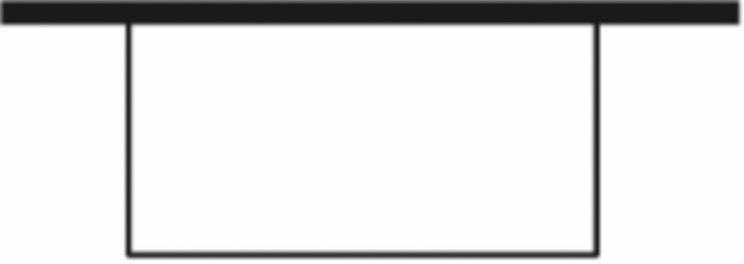
\includegraphics[width=0.28\textwidth]{figures/gao92_q8_fence.png}
\end{center}

\ifanswer
\solbegin
\step{设矩形的长为 $x$ 米，宽为 $y$，则 $xy=18$，}
\step{需要用栅栏长为 $x+2y\geqslant2\sqrt{2xy}=12$，}
\step{当且仅当 $x=2y$，即 $y=3$，$x=6$ 时取等号，故至少需要 $12$ 米栅栏.}
\solend
\fi

\item 已知 $a$ 为正整数，若关于 $x$ 的不等式 $\lvert x-2025\rvert\leqslant a$ 的解集中有且仅有 $7$ 个整数，则 $a$ 的值为\blankline[4.4em].

\ifanswer
\solbegin
\step{不等式 $\lvert x-2025\rvert\leqslant a$，则 $-a\leqslant x-2025\leqslant a$，即 $2025-a\leqslant x\leqslant2025+a$，}
\step{所以不等式 $\lvert x-2025\rvert\leqslant a$ 的解集为 $\{x\mid2025-a\leqslant x\leqslant2025+a\}$，}
\step{若不等式解集中有且仅有 $7$ 个整数，且 $a$ 为正整数，}
\step{由解集的对称性得这 $7$ 个整数以 $2025$ 为中心，向左右两边各延伸 $3$ 个整数，}
\step{即这 $7$ 个整数为 $2022,2023,2024,2025,2026,2027,2028$，所以 $a=3$.}
\solend
\fi

\item 已知关于 $x$ 的一元二次方程 $x^2-x+a=0$ 有两个不相等的正根 $m$、$n$，则 $\dfrac1m+\dfrac9n$ 的最小值为\blankline[4.4em].

\ifanswer
\solbegin
\step{因为一元二次方程 $x^2-x+a=0$ 有两个不相等的正根 $m$、$n$，}
\step{所以判别式 $\Delta=(-1)^2-4a>0\Rightarrow a<\dfrac14$，$m+n=1$，$mn=a>0$，}
\step{因此 $0<a<\dfrac14$ 且 $m+n=1(m,n>0)$.}
\step{$\dfrac1m+\dfrac9n=\left(\dfrac1m+\dfrac9n\right)(m+n)=1+\dfrac nm+\dfrac{9m}{n}+9=10+\dfrac nm+\dfrac{9m}{n}\geqslant10+2\sqrt9=16$，}
\step{等号成立条件为 $\dfrac nm=\dfrac{9m}{n}\Rightarrow n^2=9m^2\Rightarrow n=3m$，}
\step{$m$、$n>0$，结合 $m+n=1$，代入 $n=3m$ 得 $m+3m=1\Rightarrow m=\dfrac14$，$n=\dfrac34$，}
\step{此时 $mn=\dfrac14\cdot\dfrac34=\dfrac3{16}$，满足 $0<a<\dfrac14$，等号可取，因此 $\dfrac1m+\dfrac9n$ 的最小值为 $16$.}
\solend
\fi

\item 对任意 $A$、$B\subseteq R$，记 $A\oplus B=\{x\mid x\in A\cup B,x\notin A\cap B\}$，并称 $A\oplus B$ 为集合 $A$，$B$ 的对称差. 例如：若 $A=\{1,2,3\},B=\{2,3,4\}$，则 $A\oplus B=\{1,4\}$. 下列命题中，为真命题的有\blankline[4.4em].

①若 $A$、$B\subseteq R$ 且 $A\oplus B\subseteq A$，则 $A\subseteq B$

②若 $A$、$B\subseteq R$ 且 $A\oplus B=\varnothing$，则 $A=B$

③若 $A$、$B\subseteq R$ 且 $A\oplus B=B$，则 $A=\varnothing$

④对任意 $A$、$B\subseteq R$，都有 $A\oplus B=\complement_{R}A\oplus\complement_{R}B$

\ifanswer
\solbegin
\step{对于①，因为 $A\oplus B\subseteq A$，所以 $\{x\mid x\in A\cup B,x\notin A\cap B\}\subseteq A$，故 $B\subseteq A$，}
\step{故①错误；}
\step{对于②，$A$、$B\subseteq R$ 且 $A\oplus B=\varnothing$，则 $\varnothing=\{x\mid x\in A\cup B,x\notin A\cap B\}$，}
\step{即 $A\cup B=A\cap B$，所以 $A=B$，故②正确；}
\step{对于③，$A$、$B\subseteq R$ 且 $A\oplus B=B$，则 $B=\{x\mid x\in A\cup B,x\notin A\cap B\}$，}
\step{故 $A\subseteq B$，且 $B$ 中元素不在 $A\cap B$ 中，故 $A=\varnothing$，故③正确；}
\step{对于④，$\complement_{R}A\oplus\complement_{R}B=\{x\mid x\in\complement_{R}A\cup\complement_{R}B,x\notin\complement_{R}A\cap\complement_{R}B\}$，}
\step{其中 $\complement_{R}A\cup\complement_{R}B=\complement_{R}(A\cap B)$，$\complement_{R}A\cap\complement_{R}B=\complement_{R}(A\cup B)$，}
\step{故 $\complement_{R}A\oplus\complement_{R}B=\{x\mid x\in\complement_{R}(A\cap B)$，}
\step{$x\notin\complement_{R}(A\cup B)\}=\{x\mid x\in A\cup B,x\notin A\cap B\}$，}
\step{而 $A\oplus B=\{x\mid x\in A\cup B,x\notin A\cap B\}$，故 $A\oplus B=\complement_{R}A\oplus\complement_{R}B$，故④正确.}
\step{故正确的是②③④.}
\solend
\fi

\item 若不等式 $x^2-2ax+a^2-1\geqslant0$ 对任意 $x\in[0,2]$ 恒成立，则实数 $a$ 的取值范围是\blankline[4.4em].

\ifanswer
\solbegin
\step{由题意不等式 $x^2-2ax+a^2-1\geqslant0$ 对任意 $x\in[0,2]$ 恒成立，}
\step{解得 $x\leqslant a-1$ 或 $x\geqslant a+1$，要使此不等式对任意 $x\in[0,2]$ 恒成立，}
\step{则区间 $[0,2]$ 必须完全包含在解集 $(-\infty,a-1]\cup[a+1,+\infty)$ 中，}
\step{等价于 $[0,2]$ 与开区间 $(a-1,a+1)$ 的交集为空集，}
\step{区间 $[0,2]$ 在 $a-1$ 左侧，即 $2\leqslant a-1$，解得 $a\geqslant3$，}
\step{区间 $[0,2]$ 在 $a+1$ 右侧，即 $a+1\leqslant0$，解得 $a\leqslant-1$，}
\step{当 $a\in(-1,3)$，则 $(a-1,a+1)$ 与 $[0,2]$ 必有交集，不满足条件，}
\step{综上，实数 $a$ 的取值范围是 $(-\infty,-1]\cup[3,+\infty)$.}
\solend
\fi

\end{enumerate}

\bigsec{二、选择题}

\begin{enumerate}
\setcounter{enumi}{12}

\item 若 $a<b<0$，则下列不等式成立的是\mbox{（\quad）}% 原卷括号内已印“D”，试卷版按惯例留空

\keepwithprev
A. $a^2<b^2$\qquad B. $\dfrac1a<\dfrac1b$\qquad C. $ab<b^2$\qquad D. $ab<a^2$

\ifanswer
\ans{$D$}
\fi

\item 已知全集 $U=\{1,2,3,4,5\}$，集合 $A,B$ 是 $U$ 子集，满足 $\overline{A\cup B}=\{4,5\}$，$B=\{2,3\}$，则 $A\cap\overline B=\mbox{（\quad）}$

\keepwithprev
A. $\{1\}$\qquad B. $\{1,2\}$\qquad C. $\{1,4,5\}$\qquad D. $\varnothing$

\ifanswer
\solbegin
\step{因为全集 $U=\{1,2,3,4,5\}$，集合 $A$、$B$ 是 $U$ 子集，$\overline{A\cup B}=\{4,5\}$，$B=\{2,3\}$，}
\step{所以 $A\cup B=\{1,2,3\}$，故 $1\in A$，$1\notin B$，$4\notin A$，$5\notin A$，$4\notin B$，$5\notin B$，}
\step{故 $A\cap\overline B=\{1\}$. 故选 $A$.}
\solend
\fi

\item 设 $a>0$，若关于 $x$ 的不等式 $x^2-(2a-1)x-2a<0$ 的解集中恰有 $3$ 个整数，则实数 $a$ 的取值范围是\mbox{（\quad）}

\keepwithprev
A. $\left[1,\dfrac32\right]$\qquad B. $\left(1,\dfrac32\right]$\qquad C. $\left[\dfrac12,1\right]$\qquad D. $\left(\dfrac12,1\right]$

\ifanswer
\solbegin
\step{已知关于 $x$ 的不等式 $x^2-(2a-1)x-2a<0$，则 $(x+1)(x-2a)<0$，}
\step{则 $-1<x<2a$，又解集中恰有 $3$ 个整数，则 $2<2a\leqslant3$，则 $1<a\leqslant\dfrac32$，}
\step{则 $a$ 的取值范围为 $\left(1,\dfrac32\right]$. 故选 $B$.}
\solend
\fi

\item 已知集合 $U=\{1,2,3,\cdots,2027\}$，$M\subseteq U$，若对于 $M$ 中的任意两个不同的元素 $x$、$y$，都有 $\lvert x-y\rvert>2$，则 $M$ 中元素个数的最大值为\mbox{（\quad）}

\keepwithprev
A. $675$\qquad B. $676$\qquad C. $2025$\qquad D. $2026$

\ifanswer
\solbegin
\step{对于 $M$ 中的任意两个不同的元素 $x$、$y$，都有 $\lvert x-y\rvert>2$，}
\step{不妨设 $x>y$，都有 $x-y\geqslant3$，}
\step{要想 $M$ 所含元素个数最大，则要 $x-y$ 尽可能小，故需使得 $x-y$ 的最小值为 $3$，}
\step{将 $1\sim2027$ 这 $2027$ 个元素按如下分组：}
\step{$\{1,2,3\},\{4,5,6\},\cdots,\{2023,2024,2025\},\{2026,2027\}$，}
\step{故应在前 $675$ 组中按周期 $3$ 每组取一个元素，且第一组中不能取 $3$，}
\step{第一组中取 $1$ 时，得 $M=\{1,4,7,\cdots,2023,2026\}$}
\step{或 $M=\{1,4,7,\cdots,2023,2027\}$ 这样的集合，}
\step{第一组取 $2$ 时，得 $M=\{2,5,8,\cdots,2024,2027\}$，}
\step{其中任意两元素差值 $x-y(x>y)$ 都大于 $2$，满足题意，}
\step{故 $M$ 所含元素个数的最大值为 $\dfrac{2025}{3}+1=676$. 故选 $B$.}
\solend
\fi

\end{enumerate}

\bigsec{三、解答题}

\begin{enumerate}
\setcounter{enumi}{16}

\item 已知集合 $M=\{x\mid a-1\leqslant x\leqslant2a+3\}$，$P=\{x\mid-2<x\leqslant4\}$，全集 $U=R$.

（1）当 $a=2$ 时，求 $M\cap P$；

（2）若 $x\in P$ 是 $x\in M$ 的必要不充分条件，求实数 $a$ 的取值范围.

\ansspace*[9]

\ifanswer
\solbegin
\stepm{（1）}{当 $a=2$ 时，集合 $M=\{x\mid1\leqslant x\leqslant7\}$，所以 $M\cap P=\{x\mid1\leqslant x\leqslant4\}$；}
\stepm{（2）}{因为 $x\in P$ 是 $x\in M$ 的必要不充分条件，所以 $M\subsetneqq P$，}
\step{当 $M=\varnothing$ 时，$a-1>2a+3$，解得 $a<-4$，}
\step{当 $M\neq\varnothing$ 时，则 $\begin{cases}a-1\leqslant2a+3\\ a-1>-2\\ 2a+3\leqslant4\end{cases}$，解得 $-1<a\leqslant\dfrac12$，}
\step{综上所述，实数 $a$ 的取值范围为 $(-\infty,-4)\cup\left(-1,\dfrac12\right]$.}
\solend
\fi

\item 命题甲：关于 $x$ 的方程 $(a-1)x^2+(2a-4)x+a=0$ 有两个不相等的实数根；

命题乙：关于 $x$ 的不等式 $ax^2-2ax+a+1>0$ 的解集为 $R$.

（1）若命题甲为真命题，求实数 $a$ 的取值范围；

（2）若命题甲、乙中至多有一个为真命题，求实数 $a$ 的取值范围.

\ansspace*[12]

\ifanswer
\solbegin
\stepm{（1）}{命题甲：关于 $x$ 的方程 $(a-1)x^2+(2a-4)x+a=0$ 有两个不相等的实数根，}
\step{则 $\begin{cases}a-1\neq0\\ \Delta=(2a-4)^2-4a(a-1)>0\end{cases}$，解得 $a<\dfrac43$ 且 $a\neq1$，}
\step{故 $a$ 的范围为 $\left\{a\left|a<\dfrac43\ \text{且}\ a\neq1\right.\right\}$；}
\stepm{（2）}{当 $a=0$ 时 $y=1>0$，符合题意；}
\step{当 $a\neq0$，由 $\begin{cases}a>0\\ \Delta=4a^2-4a(a+1)<0\end{cases}$，解得 $a>0$，}
\step{则 $a$ 的取值范围为 $a\geqslant0$，}
\step{故 $p$、$q$ 都为真时，$a$ 的范围为 $0\leqslant a<\dfrac43$ 且 $a\neq1$，}
\step{则命题甲、乙中至多有一个为真命题时，}
\step{$a$ 的取值范围为 $\left\{a\left|a<0\ \text{或}\ a=1\ \text{或}\ a\geqslant\dfrac43\right.\right\}$.}
\solend
\fi

\item 如图，$OA$、$OB$ 是两条长度足够长的互相垂直的笔直小路，矩形 $OCPD$ 的顶点 $C$，$D$ 分别在 $OA$、$OB$ 上，且该矩形区域内种满了荷花. 为了让观赏者有更好的观赏体验，现计划经过点 $P$ 修一条小路 $EF$，其中点 $E$ 在小路 $OA$ 上，点 $F$ 在小路 $OB$ 上，并在 $\triangle OEF$ 区域内种满荷花. 已知 $OD=25$ m，$OC=40$ m，且小路 $EF$ 要完全位于一个以 $O$ 为顶点的，边长为 $100$ m 的正方形内部（包括边界）. 记 $\triangle OEF$ 的面积为 $S$ m$^2$.

\begin{center}
\begin{tikzpicture}[x=0.46cm,y=0.42cm,line width=0.7pt]
\draw (0,0) -- (0,10.2) node[above,inner sep=3pt] {$A$};
\draw (0,0) -- (11.8,0) node[right,inner sep=3pt] {$B$};
\draw (0,4.83) -- (2.42,4.83) -- (2.42,0);
\draw (0,6.92) -- (8.01,0);
\node[below left,inner sep=2pt] at (0,0) {$O$};
\node[below,inner sep=2pt] at (2.42,0) {$D$};
\node[left,inner sep=3pt] at (0,4.83) {$C$};
\node[above right,inner sep=1pt] at (2.42,4.83) {$P$};
\node[left,inner sep=3pt] at (0,6.92) {$E$};
\node[below,inner sep=2pt] at (8.01,0) {$F$};
\end{tikzpicture}
\end{center}

（1）设 $EC=x\cdot m$，试用 $x$ 表示 $OF$，并求 $x$ 的取值范围.

（2）当 $EC$ 的长度为多少时，$S$ 取得最小值？最小值是多少？

\ansspace*[11]

\ifanswer
\solbegin
\stepm{（1）}{由题意得 $x\leqslant60$，}
\step{$\triangle PCE\backsim\triangle FDP$，所以 $\dfrac{EC}{CP}=\dfrac{PD}{DF}$，即 $\dfrac{x}{25}=\dfrac{40}{DF}$，得 $DF=\dfrac{1000}{x}$ m，}
\step{所以 $OF=OD+DF=\left(25+\dfrac{1000}{x}\right)$ m，}
\step{所以 $25+\dfrac{1000}{x}\leqslant100$，解得 $x\geqslant\dfrac{40}{3}$；}
\step{综上，$\dfrac{40}{3}\leqslant x\leqslant60$；}
\stepm{（2）}{由 $OE=OC+CE=(40+x)$ m，}
\step{所以 $S=\dfrac12\cdot OF\cdot OE=\dfrac12\left(25+\dfrac{1000}{x}\right)(40+x)$}
\step{$=\dfrac12\left(1000+25x+\dfrac{40000}{x}+1000\right)$ m$^2$，}
\step{由基本不等式得 $S\geqslant\dfrac12\left(2000+2\sqrt{25x\cdot\dfrac{40000}{x}}\right)=2000$ m$^2$，}
\step{当且仅当 $25x=\dfrac{40000}{x}$，即 $x=40$ 时取等号，}
\step{故 $EC=40$ m 时，$S$ 取得最小值，为 $2000$ m$^2$.}
\solend
\fi

\item 已知函数 $f(x)=x^2-(a-2)x+a-3$.

（1）若 $f(x)=0$ 的两根为 $\alpha,\beta$，$\alpha^2+\beta^2=2$，求 $a$ 的值；

（2）解关于 $x$ 的不等式 $f(x)\geqslant0$；

（3）是否存在整数 $m,n$，使得关于 $x$ 的不等式 $m\leqslant f(x)\leqslant n$ 的解集恰好为 $[m,n]$？若存在，求出 $m,n$ 的值. 若不存在，请说明理由.

\ansspace*[16]

\ifanswer
\solbegin
\stepm{（1）}{由韦达定理，$\alpha+\beta=a-2,\alpha\beta=a-3$，}
\step{因此 $\alpha^2+\beta^2=(a-2)^2-2(a-3)=2\Leftrightarrow(a-2)(a-4)=0$，}
\step{$a=2$ 时两根为 $1,-1$；$a=4$ 时两根均为 $1$，均满足条件，}
\step{所以 $a=2$ 或 $a=4$.}
\stepm{（2）}{因为 $f(x)=(x-1)[x-(a-3)]$，所以分三种情况：}
\step{当 $a<4$ 时，$a-3<1$，解集为 $(-\infty,a-3]\cup[1,+\infty)$.}
\step{当 $a=4$ 时，$f(x)=(x-1)^2\geqslant0$ 恒成立，解集为 $R$.}
\step{当 $a>4$ 时，$a-3>1$，解集为 $(-\infty,1]\cup[a-3,+\infty)$.}
\stepm{（3）}{区间 $[m,n]$ 要求 $m<n$. 记 $f(x)$ 的最小值为 $k$.}
\step{$[m,n]$ 非空，不等式 $f(x)\leqslant n$ 有解，其解集为闭区间 $[x_1,x_2]$，}
\step{其中 $x_1\leqslant x_2$ 是方程 $f(x)=n$ 的两根.}
\step{若 $k<m$，则 $f(x)<m$ 的解集是 $[x_1,x_2]$ 内部的一个开区间，}
\step{从 $[x_1,x_2]$ 中去掉它后剩下两段，原不等式的解集不是一个区间，矛盾，}
\step{所以 $k\geqslant m$，原不等式的解集就是 $[x_1,x_2]$，于是 $m=x_1,n=x_2$，}
\step{即 $f(m)=f(n)=n$，于是 $f(m)-f(n)=(m-n)(m+n-a+2)=0$.}
\step{因为 $m\neq n$，所以 $a=m+n+2$.}
\step{代入 $f(m)=n$，得 $(m-1)(1-n)=n\Leftrightarrow m(n-1)=-1$，$m,n$ 均为整数，}
\step{因此 $(m,n)=(-1,2)$ 或 $(m,n)=(1,0)$.}
\step{结合 $m<n$，只可能有 $m=-1,n=2$，此时 $a=3$.}
\step{检验：此时 $f(x)=x^2-x$，且 $x^2-x=\left(x-\dfrac12\right)^2-\dfrac14\geqslant-\dfrac14>-1$，}
\step{因此 $-1\leqslant f(x)\leqslant2\Leftrightarrow x^2-x\leqslant2\Leftrightarrow(x+1)(x-2)\leqslant0\Leftrightarrow x\in[-1,2]$，}
\step{所以存在符合条件的整数 $m=-1,n=2$.}
\solend
\fi

\item 给定数集 $M$，若对于任意 $a$、$b\in M$，有 $a+b\in M,a-b\in M$，则称集合 $M$ 为闭集合.

（1）判断集合 $A_1=\{-4,-2,0,2,4\}$，集合 $B=\{x\mid x=3k,k\in\Z\}$ 是否为闭集合；

（2）若集合 $C$、$D$ 为闭集合，则 $C\cup D$ 是否一定为闭集合？请说明理由；

（3）已知集合 $C$、$D$ 为闭集合，且 $C\subsetneq R,D\subsetneq R$，证明：$(C\cup D)\subsetneq R$.% 原卷印作 (C∪D)⊂R，按解析证明的是 C∪D≠R，排真子集

\ansspace*[14]

\ifanswer
\solbegin
\stepm{（1）}{因为 $4\in A_1$，$2\in A_1$，$4+2=6\notin A_1$，所以 $A_1$ 不是闭集合；}
\step{任取 $x,y\in B$，设 $x=3m,y=3n,m,n\in\Z$，}
\step{则 $x+y=3m+3n=3(m+n)$ 且 $m+n\in\Z$，}
\step{所以 $x+y\in B$，同理，$x-y\in B$，故 $B$ 为闭集合.}
\stepm{（2）}{结论：不一定.}
\step{不妨令 $C=\{x\mid x=2k,k\in\Z\},D=\{x\mid x=3k,k\in\Z\}$，}
\step{则由（1）得 $C$、$D$ 为闭集合，易得 $2,3\in C\cup D,2+3=5\notin C\cup D$，}
\step{因此，$C\cup D$ 不一定是闭集合.}
\stepm{（3）}{不妨假设 $C\cup D=R$，则由 $C\subsetneq R$，得存在 $a\in R$ 且 $a\notin C$，故 $a\in D$.}
\step{同理，存在 $b\in R$ 且 $b\notin D$，故 $b\in C$.}
\step{因为 $a+b\in R=C\cup D$，所以 $a+b\in C$ 或 $a+b\in D$.}
\step{若 $a+b\in C$，则由 $C$ 为闭集合且 $b\in C$，得 $a=(a+b)-b\in C$，}
\step{与 $a\notin C$ 矛盾.}
\step{若 $a+b\in D$，则由 $D$ 为闭集合且 $a\in D$，得 $b=(a+b)-a\in D$，}
\step{与 $b\notin D$ 矛盾.}
\step{综上，$C\cup D=R$ 不成立，故 $(C\cup D)\subsetneq R$.}
\solend
\fi

\end{enumerate}

\end{document}
"
% 紧凑版：xelatex "\def\iscompact{1}% 高一92_闵行实验_10月月考.tex
%   —— 高一上数学“2026-2027 年闵行实验高一上 10 月月考”（讲评版）
% 试卷版：xelatex 高一92_闵行实验_10月月考.tex
% 答案版：xelatex "\def\isanswer{1}% 高一92_闵行实验_10月月考.tex
%   —— 高一上数学“2026-2027 年闵行实验高一上 10 月月考”（讲评版）
% 试卷版：xelatex 高一92_闵行实验_10月月考.tex
% 答案版：xelatex "\def\isanswer{1}% 高一92_闵行实验_10月月考.tex
%   —— 高一上数学“2026-2027 年闵行实验高一上 10 月月考”（讲评版）
% 试卷版：xelatex 高一92_闵行实验_10月月考.tex
% 答案版：xelatex "\def\isanswer{1}\input{高一92_闵行实验_10月月考.tex}"
% 紧凑版：xelatex "\def\iscompact{1}\input{高一92_闵行实验_10月月考.tex}"
%
% 原始材料：微信公众号“魔都数学加油站”文章，连载“27学年高一92”；
% 原文标题“27学年高一92——2026-2027年上海市闵行实验高一上10月月考”；
% 原文链接：https://mp.weixin.qq.com/s/8HUyr3G7GpcHyczwu_XYCQ。
% 正文为 10 张 PNG 页（`原图/高一92_闵行实验_10月月考/01..10.png`），均 4762×6735，按页序读取。
%
% 篇幅与题号：原卷自第 3 题起编号（第 1、2 题不在原文内）。填空题 3—12（10 题）、
% 选择题 13—16（4 题）、解答题 17—21（5 题），共 19 题。
%
% 讲评版：第 6 题只印【答案】（“$[-1,3]$”），本稿只给 \ans{}；第 13 题无【解析】、
% 答案“D”直接印在题干括号内，本稿试卷版按惯例留空、答案版提 \ans{$D$}；其余 17 题印
% 【解析】，其中选择题答案在解析末句“故选 $A$／$B$／$B$”。
% 第 8 题题干右侧有一幅“围墙 + 三面栅栏”示意图（裁自第 2 页原图）；第 19 题题干带
% 与 高一88 第 19 题同型的示意图（$OA$／$OB$ 两条小路、矩形 $OCPD$、折线 $EF$），用 TikZ 重绘。
%
% 副标题：原卷未印副标题。本稿按内容标作“集合与常用逻辑用语、不等式”。
%
% 原卷笔误/存疑（均照录未改，正文对应处另有 % 注）：
%   ① 第 21 题 (3) 题干与解析末句把结论印作“$(C\cup D)\subset R$”，而解析证明的是
%      “$C\cup D=\R$ 不成立”，按文意应为“$(C\cup D)\subsetneq\R$”；本稿按真子集排
%      $\subsetneq$，原卷记号照录于文件头；
%   ② 第 7 题解析只列 $B=\varnothing$（$a=0$）、$B=\{1\}$（$a=1$）、$B=\{-3\}$（$a=-\frac13$）
%      三种情形，与结论 $\left\{0,1,-\frac13\right\}$ 相符，无笔误。
%
% 与原卷的排版差异：
%   ① 原卷每题下直接印【答案】/【解析】，本稿按全稿惯例将答案与解析置于答案版；
%   ② 原卷未印副标题，本稿补出；填空横线统一排 \blankline[4.4em]；
%   ③ 原卷数集记号排斜体 $R$、$Z$，本稿按全稿惯例改用 $\R$、$\Z$；
%   ④ 第 17—21 题的子问用行内“（1）（2）（3）”段，解析中的子问标号用 \stepm；
%   ⑤ 解答题按惯例加 \ansspace；选择题括号排 \mbox{（\quad）}；
%   ⑥ 第 8 题的示意图原卷排在题干右侧、文字绕排，本稿改排为题干后的居中图
%      （自原图裁切、去粉色水印后转灰度）；第 19 题的图按原图比例 TikZ 重绘。
%
% 行数核对：逐题数 \step/\stepm 条数，合计 128 条（Q3：2；Q4：3；Q5：2；Q6：0；Q7：6；
% Q8：3；Q9：5；Q10：7；Q11：12；Q12：8；Q13：0；Q14：3；Q15：3；Q16：11；Q17：5；
% Q18：9；Q19：11；Q20：22；Q21：16）。第 6 题只印答案、第 13 题无解析，均不计入 \step 账。
% 原卷解析的换行按语意合并，未逐行强拆。
%
\documentclass[a4paper,11pt]{article}
\usepackage{common}

\begin{document}

\examtitlest[7]{2026--2027 年闵行实验高一上 10 月月考}{集合与常用逻辑用语、不等式}

\bigsec{一、填空题}

\begin{enumerate}
\setcounter{enumi}{2}

\item 已知 $3<a<8$，$4<b<9$，则 $\dfrac ab$ 的取值范围是\blankline[4.4em].

\ifanswer
\solbegin
\step{因为 $4<b<9$，所以 $\dfrac19<\dfrac1b<\dfrac14$，又 $3<a<8$，所以 $\dfrac13<\dfrac ab<2$，}
\step{故 $\dfrac ab$ 的取值范围是 $\left(\dfrac13,2\right)$.}
\solend
\fi

\item 已知 $p:x>3$，$q:x>5$，则 $p$ 是 $q$ 的\blankline[4.4em]（选“充分不必要条件”“必要不充分条件”“充要条件”“既不充分也不必要条件”之一填空）.

\ifanswer
\solbegin
\step{当 $x>3$ 时，不能推出 $x>5$，充分性不成立；}
\step{当 $x>5$ 时，可以得到 $x>3$，必要性成立；}
\step{故 $p$ 是 $q$ 的必要不充分条件.}
\solend
\fi

\item 不等式 $\dfrac{x-1}{2x+1}\leqslant1$ 的解集为\blankline[4.4em].

\ifanswer
\solbegin
\step{因为 $\dfrac{x-1}{2x+1}\leqslant1$，所以 $\dfrac{x-1}{2x+1}-\dfrac{2x+1}{2x+1}\leqslant0$，所以 $\dfrac{x+2}{2x+1}\geqslant0$，}
\step{所以 $x>-\dfrac12$ 或 $x\leqslant-2$，即不等式的解集是 $(-\infty,-2]\cup\left(-\dfrac12,+\infty\right)$.}
\solend
\fi

\item 设 $x\in R$，则方程 $\lvert x+1\rvert+\lvert x-3\rvert=4$ 的解集为\blankline[4.4em].

\ifanswer
\ans{$[-1,3]$}
\fi

\item 若 $A=\{x\mid x^2+2x=3\}$，$B=\{x\mid ax=1\}$，且 $B\subseteq A$，则实数 $a$ 的值组成的集合为\blankline[4.4em].

\ifanswer
\solbegin
\step{由 $x^2+2x=3$ 得 $x^2+2x-3=0$，解得 $x=1$ 或 $x=-3$，所以 $A=\{1,-3\}$，}
\step{又因为 $B=\{x\mid ax=1\}$，且 $B\subseteq A$，}
\step{当 $B=\varnothing$，即 $a=0$ 时，显然符合题意；}
\step{当 $B=\{1\}$，即 $a=1$ 时，也符合题意；}
\step{当 $B=\{-3\}$，即 $a=-\dfrac13$ 时，也符合题意；}
\step{综上所述，实数 $a$ 的值组成的集合为 $\left\{0,1,-\dfrac13\right\}$.}
\solend
\fi

\item 某校欲在围墙边用栅栏围成一个 $18$ 平方米的矩形区域，作为天鹅的地面栖息地，矩形区域的一条边为围墙（如图），则至少需要\blankline[4.4em]米栅栏.

\begin{center}
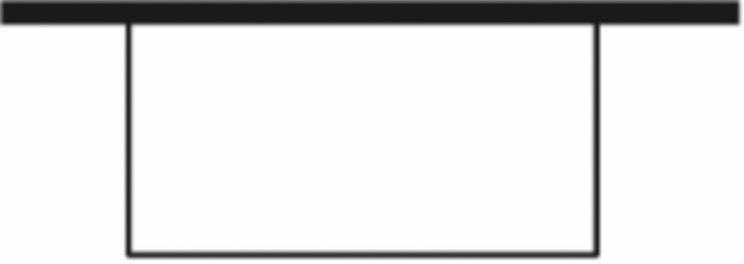
\includegraphics[width=0.28\textwidth]{figures/gao92_q8_fence.png}
\end{center}

\ifanswer
\solbegin
\step{设矩形的长为 $x$ 米，宽为 $y$，则 $xy=18$，}
\step{需要用栅栏长为 $x+2y\geqslant2\sqrt{2xy}=12$，}
\step{当且仅当 $x=2y$，即 $y=3$，$x=6$ 时取等号，故至少需要 $12$ 米栅栏.}
\solend
\fi

\item 已知 $a$ 为正整数，若关于 $x$ 的不等式 $\lvert x-2025\rvert\leqslant a$ 的解集中有且仅有 $7$ 个整数，则 $a$ 的值为\blankline[4.4em].

\ifanswer
\solbegin
\step{不等式 $\lvert x-2025\rvert\leqslant a$，则 $-a\leqslant x-2025\leqslant a$，即 $2025-a\leqslant x\leqslant2025+a$，}
\step{所以不等式 $\lvert x-2025\rvert\leqslant a$ 的解集为 $\{x\mid2025-a\leqslant x\leqslant2025+a\}$，}
\step{若不等式解集中有且仅有 $7$ 个整数，且 $a$ 为正整数，}
\step{由解集的对称性得这 $7$ 个整数以 $2025$ 为中心，向左右两边各延伸 $3$ 个整数，}
\step{即这 $7$ 个整数为 $2022,2023,2024,2025,2026,2027,2028$，所以 $a=3$.}
\solend
\fi

\item 已知关于 $x$ 的一元二次方程 $x^2-x+a=0$ 有两个不相等的正根 $m$、$n$，则 $\dfrac1m+\dfrac9n$ 的最小值为\blankline[4.4em].

\ifanswer
\solbegin
\step{因为一元二次方程 $x^2-x+a=0$ 有两个不相等的正根 $m$、$n$，}
\step{所以判别式 $\Delta=(-1)^2-4a>0\Rightarrow a<\dfrac14$，$m+n=1$，$mn=a>0$，}
\step{因此 $0<a<\dfrac14$ 且 $m+n=1(m,n>0)$.}
\step{$\dfrac1m+\dfrac9n=\left(\dfrac1m+\dfrac9n\right)(m+n)=1+\dfrac nm+\dfrac{9m}{n}+9=10+\dfrac nm+\dfrac{9m}{n}\geqslant10+2\sqrt9=16$，}
\step{等号成立条件为 $\dfrac nm=\dfrac{9m}{n}\Rightarrow n^2=9m^2\Rightarrow n=3m$，}
\step{$m$、$n>0$，结合 $m+n=1$，代入 $n=3m$ 得 $m+3m=1\Rightarrow m=\dfrac14$，$n=\dfrac34$，}
\step{此时 $mn=\dfrac14\cdot\dfrac34=\dfrac3{16}$，满足 $0<a<\dfrac14$，等号可取，因此 $\dfrac1m+\dfrac9n$ 的最小值为 $16$.}
\solend
\fi

\item 对任意 $A$、$B\subseteq R$，记 $A\oplus B=\{x\mid x\in A\cup B,x\notin A\cap B\}$，并称 $A\oplus B$ 为集合 $A$，$B$ 的对称差. 例如：若 $A=\{1,2,3\},B=\{2,3,4\}$，则 $A\oplus B=\{1,4\}$. 下列命题中，为真命题的有\blankline[4.4em].

①若 $A$、$B\subseteq R$ 且 $A\oplus B\subseteq A$，则 $A\subseteq B$

②若 $A$、$B\subseteq R$ 且 $A\oplus B=\varnothing$，则 $A=B$

③若 $A$、$B\subseteq R$ 且 $A\oplus B=B$，则 $A=\varnothing$

④对任意 $A$、$B\subseteq R$，都有 $A\oplus B=\complement_{R}A\oplus\complement_{R}B$

\ifanswer
\solbegin
\step{对于①，因为 $A\oplus B\subseteq A$，所以 $\{x\mid x\in A\cup B,x\notin A\cap B\}\subseteq A$，故 $B\subseteq A$，}
\step{故①错误；}
\step{对于②，$A$、$B\subseteq R$ 且 $A\oplus B=\varnothing$，则 $\varnothing=\{x\mid x\in A\cup B,x\notin A\cap B\}$，}
\step{即 $A\cup B=A\cap B$，所以 $A=B$，故②正确；}
\step{对于③，$A$、$B\subseteq R$ 且 $A\oplus B=B$，则 $B=\{x\mid x\in A\cup B,x\notin A\cap B\}$，}
\step{故 $A\subseteq B$，且 $B$ 中元素不在 $A\cap B$ 中，故 $A=\varnothing$，故③正确；}
\step{对于④，$\complement_{R}A\oplus\complement_{R}B=\{x\mid x\in\complement_{R}A\cup\complement_{R}B,x\notin\complement_{R}A\cap\complement_{R}B\}$，}
\step{其中 $\complement_{R}A\cup\complement_{R}B=\complement_{R}(A\cap B)$，$\complement_{R}A\cap\complement_{R}B=\complement_{R}(A\cup B)$，}
\step{故 $\complement_{R}A\oplus\complement_{R}B=\{x\mid x\in\complement_{R}(A\cap B)$，}
\step{$x\notin\complement_{R}(A\cup B)\}=\{x\mid x\in A\cup B,x\notin A\cap B\}$，}
\step{而 $A\oplus B=\{x\mid x\in A\cup B,x\notin A\cap B\}$，故 $A\oplus B=\complement_{R}A\oplus\complement_{R}B$，故④正确.}
\step{故正确的是②③④.}
\solend
\fi

\item 若不等式 $x^2-2ax+a^2-1\geqslant0$ 对任意 $x\in[0,2]$ 恒成立，则实数 $a$ 的取值范围是\blankline[4.4em].

\ifanswer
\solbegin
\step{由题意不等式 $x^2-2ax+a^2-1\geqslant0$ 对任意 $x\in[0,2]$ 恒成立，}
\step{解得 $x\leqslant a-1$ 或 $x\geqslant a+1$，要使此不等式对任意 $x\in[0,2]$ 恒成立，}
\step{则区间 $[0,2]$ 必须完全包含在解集 $(-\infty,a-1]\cup[a+1,+\infty)$ 中，}
\step{等价于 $[0,2]$ 与开区间 $(a-1,a+1)$ 的交集为空集，}
\step{区间 $[0,2]$ 在 $a-1$ 左侧，即 $2\leqslant a-1$，解得 $a\geqslant3$，}
\step{区间 $[0,2]$ 在 $a+1$ 右侧，即 $a+1\leqslant0$，解得 $a\leqslant-1$，}
\step{当 $a\in(-1,3)$，则 $(a-1,a+1)$ 与 $[0,2]$ 必有交集，不满足条件，}
\step{综上，实数 $a$ 的取值范围是 $(-\infty,-1]\cup[3,+\infty)$.}
\solend
\fi

\end{enumerate}

\bigsec{二、选择题}

\begin{enumerate}
\setcounter{enumi}{12}

\item 若 $a<b<0$，则下列不等式成立的是\mbox{（\quad）}% 原卷括号内已印“D”，试卷版按惯例留空

\keepwithprev
A. $a^2<b^2$\qquad B. $\dfrac1a<\dfrac1b$\qquad C. $ab<b^2$\qquad D. $ab<a^2$

\ifanswer
\ans{$D$}
\fi

\item 已知全集 $U=\{1,2,3,4,5\}$，集合 $A,B$ 是 $U$ 子集，满足 $\overline{A\cup B}=\{4,5\}$，$B=\{2,3\}$，则 $A\cap\overline B=\mbox{（\quad）}$

\keepwithprev
A. $\{1\}$\qquad B. $\{1,2\}$\qquad C. $\{1,4,5\}$\qquad D. $\varnothing$

\ifanswer
\solbegin
\step{因为全集 $U=\{1,2,3,4,5\}$，集合 $A$、$B$ 是 $U$ 子集，$\overline{A\cup B}=\{4,5\}$，$B=\{2,3\}$，}
\step{所以 $A\cup B=\{1,2,3\}$，故 $1\in A$，$1\notin B$，$4\notin A$，$5\notin A$，$4\notin B$，$5\notin B$，}
\step{故 $A\cap\overline B=\{1\}$. 故选 $A$.}
\solend
\fi

\item 设 $a>0$，若关于 $x$ 的不等式 $x^2-(2a-1)x-2a<0$ 的解集中恰有 $3$ 个整数，则实数 $a$ 的取值范围是\mbox{（\quad）}

\keepwithprev
A. $\left[1,\dfrac32\right]$\qquad B. $\left(1,\dfrac32\right]$\qquad C. $\left[\dfrac12,1\right]$\qquad D. $\left(\dfrac12,1\right]$

\ifanswer
\solbegin
\step{已知关于 $x$ 的不等式 $x^2-(2a-1)x-2a<0$，则 $(x+1)(x-2a)<0$，}
\step{则 $-1<x<2a$，又解集中恰有 $3$ 个整数，则 $2<2a\leqslant3$，则 $1<a\leqslant\dfrac32$，}
\step{则 $a$ 的取值范围为 $\left(1,\dfrac32\right]$. 故选 $B$.}
\solend
\fi

\item 已知集合 $U=\{1,2,3,\cdots,2027\}$，$M\subseteq U$，若对于 $M$ 中的任意两个不同的元素 $x$、$y$，都有 $\lvert x-y\rvert>2$，则 $M$ 中元素个数的最大值为\mbox{（\quad）}

\keepwithprev
A. $675$\qquad B. $676$\qquad C. $2025$\qquad D. $2026$

\ifanswer
\solbegin
\step{对于 $M$ 中的任意两个不同的元素 $x$、$y$，都有 $\lvert x-y\rvert>2$，}
\step{不妨设 $x>y$，都有 $x-y\geqslant3$，}
\step{要想 $M$ 所含元素个数最大，则要 $x-y$ 尽可能小，故需使得 $x-y$ 的最小值为 $3$，}
\step{将 $1\sim2027$ 这 $2027$ 个元素按如下分组：}
\step{$\{1,2,3\},\{4,5,6\},\cdots,\{2023,2024,2025\},\{2026,2027\}$，}
\step{故应在前 $675$ 组中按周期 $3$ 每组取一个元素，且第一组中不能取 $3$，}
\step{第一组中取 $1$ 时，得 $M=\{1,4,7,\cdots,2023,2026\}$}
\step{或 $M=\{1,4,7,\cdots,2023,2027\}$ 这样的集合，}
\step{第一组取 $2$ 时，得 $M=\{2,5,8,\cdots,2024,2027\}$，}
\step{其中任意两元素差值 $x-y(x>y)$ 都大于 $2$，满足题意，}
\step{故 $M$ 所含元素个数的最大值为 $\dfrac{2025}{3}+1=676$. 故选 $B$.}
\solend
\fi

\end{enumerate}

\bigsec{三、解答题}

\begin{enumerate}
\setcounter{enumi}{16}

\item 已知集合 $M=\{x\mid a-1\leqslant x\leqslant2a+3\}$，$P=\{x\mid-2<x\leqslant4\}$，全集 $U=R$.

（1）当 $a=2$ 时，求 $M\cap P$；

（2）若 $x\in P$ 是 $x\in M$ 的必要不充分条件，求实数 $a$ 的取值范围.

\ansspace*[9]

\ifanswer
\solbegin
\stepm{（1）}{当 $a=2$ 时，集合 $M=\{x\mid1\leqslant x\leqslant7\}$，所以 $M\cap P=\{x\mid1\leqslant x\leqslant4\}$；}
\stepm{（2）}{因为 $x\in P$ 是 $x\in M$ 的必要不充分条件，所以 $M\subsetneqq P$，}
\step{当 $M=\varnothing$ 时，$a-1>2a+3$，解得 $a<-4$，}
\step{当 $M\neq\varnothing$ 时，则 $\begin{cases}a-1\leqslant2a+3\\ a-1>-2\\ 2a+3\leqslant4\end{cases}$，解得 $-1<a\leqslant\dfrac12$，}
\step{综上所述，实数 $a$ 的取值范围为 $(-\infty,-4)\cup\left(-1,\dfrac12\right]$.}
\solend
\fi

\item 命题甲：关于 $x$ 的方程 $(a-1)x^2+(2a-4)x+a=0$ 有两个不相等的实数根；

命题乙：关于 $x$ 的不等式 $ax^2-2ax+a+1>0$ 的解集为 $R$.

（1）若命题甲为真命题，求实数 $a$ 的取值范围；

（2）若命题甲、乙中至多有一个为真命题，求实数 $a$ 的取值范围.

\ansspace*[12]

\ifanswer
\solbegin
\stepm{（1）}{命题甲：关于 $x$ 的方程 $(a-1)x^2+(2a-4)x+a=0$ 有两个不相等的实数根，}
\step{则 $\begin{cases}a-1\neq0\\ \Delta=(2a-4)^2-4a(a-1)>0\end{cases}$，解得 $a<\dfrac43$ 且 $a\neq1$，}
\step{故 $a$ 的范围为 $\left\{a\left|a<\dfrac43\ \text{且}\ a\neq1\right.\right\}$；}
\stepm{（2）}{当 $a=0$ 时 $y=1>0$，符合题意；}
\step{当 $a\neq0$，由 $\begin{cases}a>0\\ \Delta=4a^2-4a(a+1)<0\end{cases}$，解得 $a>0$，}
\step{则 $a$ 的取值范围为 $a\geqslant0$，}
\step{故 $p$、$q$ 都为真时，$a$ 的范围为 $0\leqslant a<\dfrac43$ 且 $a\neq1$，}
\step{则命题甲、乙中至多有一个为真命题时，}
\step{$a$ 的取值范围为 $\left\{a\left|a<0\ \text{或}\ a=1\ \text{或}\ a\geqslant\dfrac43\right.\right\}$.}
\solend
\fi

\item 如图，$OA$、$OB$ 是两条长度足够长的互相垂直的笔直小路，矩形 $OCPD$ 的顶点 $C$，$D$ 分别在 $OA$、$OB$ 上，且该矩形区域内种满了荷花. 为了让观赏者有更好的观赏体验，现计划经过点 $P$ 修一条小路 $EF$，其中点 $E$ 在小路 $OA$ 上，点 $F$ 在小路 $OB$ 上，并在 $\triangle OEF$ 区域内种满荷花. 已知 $OD=25$ m，$OC=40$ m，且小路 $EF$ 要完全位于一个以 $O$ 为顶点的，边长为 $100$ m 的正方形内部（包括边界）. 记 $\triangle OEF$ 的面积为 $S$ m$^2$.

\begin{center}
\begin{tikzpicture}[x=0.46cm,y=0.42cm,line width=0.7pt]
\draw (0,0) -- (0,10.2) node[above,inner sep=3pt] {$A$};
\draw (0,0) -- (11.8,0) node[right,inner sep=3pt] {$B$};
\draw (0,4.83) -- (2.42,4.83) -- (2.42,0);
\draw (0,6.92) -- (8.01,0);
\node[below left,inner sep=2pt] at (0,0) {$O$};
\node[below,inner sep=2pt] at (2.42,0) {$D$};
\node[left,inner sep=3pt] at (0,4.83) {$C$};
\node[above right,inner sep=1pt] at (2.42,4.83) {$P$};
\node[left,inner sep=3pt] at (0,6.92) {$E$};
\node[below,inner sep=2pt] at (8.01,0) {$F$};
\end{tikzpicture}
\end{center}

（1）设 $EC=x\cdot m$，试用 $x$ 表示 $OF$，并求 $x$ 的取值范围.

（2）当 $EC$ 的长度为多少时，$S$ 取得最小值？最小值是多少？

\ansspace*[11]

\ifanswer
\solbegin
\stepm{（1）}{由题意得 $x\leqslant60$，}
\step{$\triangle PCE\backsim\triangle FDP$，所以 $\dfrac{EC}{CP}=\dfrac{PD}{DF}$，即 $\dfrac{x}{25}=\dfrac{40}{DF}$，得 $DF=\dfrac{1000}{x}$ m，}
\step{所以 $OF=OD+DF=\left(25+\dfrac{1000}{x}\right)$ m，}
\step{所以 $25+\dfrac{1000}{x}\leqslant100$，解得 $x\geqslant\dfrac{40}{3}$；}
\step{综上，$\dfrac{40}{3}\leqslant x\leqslant60$；}
\stepm{（2）}{由 $OE=OC+CE=(40+x)$ m，}
\step{所以 $S=\dfrac12\cdot OF\cdot OE=\dfrac12\left(25+\dfrac{1000}{x}\right)(40+x)$}
\step{$=\dfrac12\left(1000+25x+\dfrac{40000}{x}+1000\right)$ m$^2$，}
\step{由基本不等式得 $S\geqslant\dfrac12\left(2000+2\sqrt{25x\cdot\dfrac{40000}{x}}\right)=2000$ m$^2$，}
\step{当且仅当 $25x=\dfrac{40000}{x}$，即 $x=40$ 时取等号，}
\step{故 $EC=40$ m 时，$S$ 取得最小值，为 $2000$ m$^2$.}
\solend
\fi

\item 已知函数 $f(x)=x^2-(a-2)x+a-3$.

（1）若 $f(x)=0$ 的两根为 $\alpha,\beta$，$\alpha^2+\beta^2=2$，求 $a$ 的值；

（2）解关于 $x$ 的不等式 $f(x)\geqslant0$；

（3）是否存在整数 $m,n$，使得关于 $x$ 的不等式 $m\leqslant f(x)\leqslant n$ 的解集恰好为 $[m,n]$？若存在，求出 $m,n$ 的值. 若不存在，请说明理由.

\ansspace*[16]

\ifanswer
\solbegin
\stepm{（1）}{由韦达定理，$\alpha+\beta=a-2,\alpha\beta=a-3$，}
\step{因此 $\alpha^2+\beta^2=(a-2)^2-2(a-3)=2\Leftrightarrow(a-2)(a-4)=0$，}
\step{$a=2$ 时两根为 $1,-1$；$a=4$ 时两根均为 $1$，均满足条件，}
\step{所以 $a=2$ 或 $a=4$.}
\stepm{（2）}{因为 $f(x)=(x-1)[x-(a-3)]$，所以分三种情况：}
\step{当 $a<4$ 时，$a-3<1$，解集为 $(-\infty,a-3]\cup[1,+\infty)$.}
\step{当 $a=4$ 时，$f(x)=(x-1)^2\geqslant0$ 恒成立，解集为 $R$.}
\step{当 $a>4$ 时，$a-3>1$，解集为 $(-\infty,1]\cup[a-3,+\infty)$.}
\stepm{（3）}{区间 $[m,n]$ 要求 $m<n$. 记 $f(x)$ 的最小值为 $k$.}
\step{$[m,n]$ 非空，不等式 $f(x)\leqslant n$ 有解，其解集为闭区间 $[x_1,x_2]$，}
\step{其中 $x_1\leqslant x_2$ 是方程 $f(x)=n$ 的两根.}
\step{若 $k<m$，则 $f(x)<m$ 的解集是 $[x_1,x_2]$ 内部的一个开区间，}
\step{从 $[x_1,x_2]$ 中去掉它后剩下两段，原不等式的解集不是一个区间，矛盾，}
\step{所以 $k\geqslant m$，原不等式的解集就是 $[x_1,x_2]$，于是 $m=x_1,n=x_2$，}
\step{即 $f(m)=f(n)=n$，于是 $f(m)-f(n)=(m-n)(m+n-a+2)=0$.}
\step{因为 $m\neq n$，所以 $a=m+n+2$.}
\step{代入 $f(m)=n$，得 $(m-1)(1-n)=n\Leftrightarrow m(n-1)=-1$，$m,n$ 均为整数，}
\step{因此 $(m,n)=(-1,2)$ 或 $(m,n)=(1,0)$.}
\step{结合 $m<n$，只可能有 $m=-1,n=2$，此时 $a=3$.}
\step{检验：此时 $f(x)=x^2-x$，且 $x^2-x=\left(x-\dfrac12\right)^2-\dfrac14\geqslant-\dfrac14>-1$，}
\step{因此 $-1\leqslant f(x)\leqslant2\Leftrightarrow x^2-x\leqslant2\Leftrightarrow(x+1)(x-2)\leqslant0\Leftrightarrow x\in[-1,2]$，}
\step{所以存在符合条件的整数 $m=-1,n=2$.}
\solend
\fi

\item 给定数集 $M$，若对于任意 $a$、$b\in M$，有 $a+b\in M,a-b\in M$，则称集合 $M$ 为闭集合.

（1）判断集合 $A_1=\{-4,-2,0,2,4\}$，集合 $B=\{x\mid x=3k,k\in\Z\}$ 是否为闭集合；

（2）若集合 $C$、$D$ 为闭集合，则 $C\cup D$ 是否一定为闭集合？请说明理由；

（3）已知集合 $C$、$D$ 为闭集合，且 $C\subsetneq R,D\subsetneq R$，证明：$(C\cup D)\subsetneq R$.% 原卷印作 (C∪D)⊂R，按解析证明的是 C∪D≠R，排真子集

\ansspace*[14]

\ifanswer
\solbegin
\stepm{（1）}{因为 $4\in A_1$，$2\in A_1$，$4+2=6\notin A_1$，所以 $A_1$ 不是闭集合；}
\step{任取 $x,y\in B$，设 $x=3m,y=3n,m,n\in\Z$，}
\step{则 $x+y=3m+3n=3(m+n)$ 且 $m+n\in\Z$，}
\step{所以 $x+y\in B$，同理，$x-y\in B$，故 $B$ 为闭集合.}
\stepm{（2）}{结论：不一定.}
\step{不妨令 $C=\{x\mid x=2k,k\in\Z\},D=\{x\mid x=3k,k\in\Z\}$，}
\step{则由（1）得 $C$、$D$ 为闭集合，易得 $2,3\in C\cup D,2+3=5\notin C\cup D$，}
\step{因此，$C\cup D$ 不一定是闭集合.}
\stepm{（3）}{不妨假设 $C\cup D=R$，则由 $C\subsetneq R$，得存在 $a\in R$ 且 $a\notin C$，故 $a\in D$.}
\step{同理，存在 $b\in R$ 且 $b\notin D$，故 $b\in C$.}
\step{因为 $a+b\in R=C\cup D$，所以 $a+b\in C$ 或 $a+b\in D$.}
\step{若 $a+b\in C$，则由 $C$ 为闭集合且 $b\in C$，得 $a=(a+b)-b\in C$，}
\step{与 $a\notin C$ 矛盾.}
\step{若 $a+b\in D$，则由 $D$ 为闭集合且 $a\in D$，得 $b=(a+b)-a\in D$，}
\step{与 $b\notin D$ 矛盾.}
\step{综上，$C\cup D=R$ 不成立，故 $(C\cup D)\subsetneq R$.}
\solend
\fi

\end{enumerate}

\end{document}
"
% 紧凑版：xelatex "\def\iscompact{1}% 高一92_闵行实验_10月月考.tex
%   —— 高一上数学“2026-2027 年闵行实验高一上 10 月月考”（讲评版）
% 试卷版：xelatex 高一92_闵行实验_10月月考.tex
% 答案版：xelatex "\def\isanswer{1}\input{高一92_闵行实验_10月月考.tex}"
% 紧凑版：xelatex "\def\iscompact{1}\input{高一92_闵行实验_10月月考.tex}"
%
% 原始材料：微信公众号“魔都数学加油站”文章，连载“27学年高一92”；
% 原文标题“27学年高一92——2026-2027年上海市闵行实验高一上10月月考”；
% 原文链接：https://mp.weixin.qq.com/s/8HUyr3G7GpcHyczwu_XYCQ。
% 正文为 10 张 PNG 页（`原图/高一92_闵行实验_10月月考/01..10.png`），均 4762×6735，按页序读取。
%
% 篇幅与题号：原卷自第 3 题起编号（第 1、2 题不在原文内）。填空题 3—12（10 题）、
% 选择题 13—16（4 题）、解答题 17—21（5 题），共 19 题。
%
% 讲评版：第 6 题只印【答案】（“$[-1,3]$”），本稿只给 \ans{}；第 13 题无【解析】、
% 答案“D”直接印在题干括号内，本稿试卷版按惯例留空、答案版提 \ans{$D$}；其余 17 题印
% 【解析】，其中选择题答案在解析末句“故选 $A$／$B$／$B$”。
% 第 8 题题干右侧有一幅“围墙 + 三面栅栏”示意图（裁自第 2 页原图）；第 19 题题干带
% 与 高一88 第 19 题同型的示意图（$OA$／$OB$ 两条小路、矩形 $OCPD$、折线 $EF$），用 TikZ 重绘。
%
% 副标题：原卷未印副标题。本稿按内容标作“集合与常用逻辑用语、不等式”。
%
% 原卷笔误/存疑（均照录未改，正文对应处另有 % 注）：
%   ① 第 21 题 (3) 题干与解析末句把结论印作“$(C\cup D)\subset R$”，而解析证明的是
%      “$C\cup D=\R$ 不成立”，按文意应为“$(C\cup D)\subsetneq\R$”；本稿按真子集排
%      $\subsetneq$，原卷记号照录于文件头；
%   ② 第 7 题解析只列 $B=\varnothing$（$a=0$）、$B=\{1\}$（$a=1$）、$B=\{-3\}$（$a=-\frac13$）
%      三种情形，与结论 $\left\{0,1,-\frac13\right\}$ 相符，无笔误。
%
% 与原卷的排版差异：
%   ① 原卷每题下直接印【答案】/【解析】，本稿按全稿惯例将答案与解析置于答案版；
%   ② 原卷未印副标题，本稿补出；填空横线统一排 \blankline[4.4em]；
%   ③ 原卷数集记号排斜体 $R$、$Z$，本稿按全稿惯例改用 $\R$、$\Z$；
%   ④ 第 17—21 题的子问用行内“（1）（2）（3）”段，解析中的子问标号用 \stepm；
%   ⑤ 解答题按惯例加 \ansspace；选择题括号排 \mbox{（\quad）}；
%   ⑥ 第 8 题的示意图原卷排在题干右侧、文字绕排，本稿改排为题干后的居中图
%      （自原图裁切、去粉色水印后转灰度）；第 19 题的图按原图比例 TikZ 重绘。
%
% 行数核对：逐题数 \step/\stepm 条数，合计 128 条（Q3：2；Q4：3；Q5：2；Q6：0；Q7：6；
% Q8：3；Q9：5；Q10：7；Q11：12；Q12：8；Q13：0；Q14：3；Q15：3；Q16：11；Q17：5；
% Q18：9；Q19：11；Q20：22；Q21：16）。第 6 题只印答案、第 13 题无解析，均不计入 \step 账。
% 原卷解析的换行按语意合并，未逐行强拆。
%
\documentclass[a4paper,11pt]{article}
\usepackage{common}

\begin{document}

\examtitlest[7]{2026--2027 年闵行实验高一上 10 月月考}{集合与常用逻辑用语、不等式}

\bigsec{一、填空题}

\begin{enumerate}
\setcounter{enumi}{2}

\item 已知 $3<a<8$，$4<b<9$，则 $\dfrac ab$ 的取值范围是\blankline[4.4em].

\ifanswer
\solbegin
\step{因为 $4<b<9$，所以 $\dfrac19<\dfrac1b<\dfrac14$，又 $3<a<8$，所以 $\dfrac13<\dfrac ab<2$，}
\step{故 $\dfrac ab$ 的取值范围是 $\left(\dfrac13,2\right)$.}
\solend
\fi

\item 已知 $p:x>3$，$q:x>5$，则 $p$ 是 $q$ 的\blankline[4.4em]（选“充分不必要条件”“必要不充分条件”“充要条件”“既不充分也不必要条件”之一填空）.

\ifanswer
\solbegin
\step{当 $x>3$ 时，不能推出 $x>5$，充分性不成立；}
\step{当 $x>5$ 时，可以得到 $x>3$，必要性成立；}
\step{故 $p$ 是 $q$ 的必要不充分条件.}
\solend
\fi

\item 不等式 $\dfrac{x-1}{2x+1}\leqslant1$ 的解集为\blankline[4.4em].

\ifanswer
\solbegin
\step{因为 $\dfrac{x-1}{2x+1}\leqslant1$，所以 $\dfrac{x-1}{2x+1}-\dfrac{2x+1}{2x+1}\leqslant0$，所以 $\dfrac{x+2}{2x+1}\geqslant0$，}
\step{所以 $x>-\dfrac12$ 或 $x\leqslant-2$，即不等式的解集是 $(-\infty,-2]\cup\left(-\dfrac12,+\infty\right)$.}
\solend
\fi

\item 设 $x\in R$，则方程 $\lvert x+1\rvert+\lvert x-3\rvert=4$ 的解集为\blankline[4.4em].

\ifanswer
\ans{$[-1,3]$}
\fi

\item 若 $A=\{x\mid x^2+2x=3\}$，$B=\{x\mid ax=1\}$，且 $B\subseteq A$，则实数 $a$ 的值组成的集合为\blankline[4.4em].

\ifanswer
\solbegin
\step{由 $x^2+2x=3$ 得 $x^2+2x-3=0$，解得 $x=1$ 或 $x=-3$，所以 $A=\{1,-3\}$，}
\step{又因为 $B=\{x\mid ax=1\}$，且 $B\subseteq A$，}
\step{当 $B=\varnothing$，即 $a=0$ 时，显然符合题意；}
\step{当 $B=\{1\}$，即 $a=1$ 时，也符合题意；}
\step{当 $B=\{-3\}$，即 $a=-\dfrac13$ 时，也符合题意；}
\step{综上所述，实数 $a$ 的值组成的集合为 $\left\{0,1,-\dfrac13\right\}$.}
\solend
\fi

\item 某校欲在围墙边用栅栏围成一个 $18$ 平方米的矩形区域，作为天鹅的地面栖息地，矩形区域的一条边为围墙（如图），则至少需要\blankline[4.4em]米栅栏.

\begin{center}
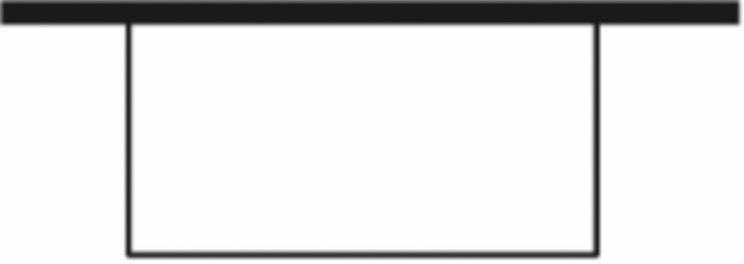
\includegraphics[width=0.28\textwidth]{figures/gao92_q8_fence.png}
\end{center}

\ifanswer
\solbegin
\step{设矩形的长为 $x$ 米，宽为 $y$，则 $xy=18$，}
\step{需要用栅栏长为 $x+2y\geqslant2\sqrt{2xy}=12$，}
\step{当且仅当 $x=2y$，即 $y=3$，$x=6$ 时取等号，故至少需要 $12$ 米栅栏.}
\solend
\fi

\item 已知 $a$ 为正整数，若关于 $x$ 的不等式 $\lvert x-2025\rvert\leqslant a$ 的解集中有且仅有 $7$ 个整数，则 $a$ 的值为\blankline[4.4em].

\ifanswer
\solbegin
\step{不等式 $\lvert x-2025\rvert\leqslant a$，则 $-a\leqslant x-2025\leqslant a$，即 $2025-a\leqslant x\leqslant2025+a$，}
\step{所以不等式 $\lvert x-2025\rvert\leqslant a$ 的解集为 $\{x\mid2025-a\leqslant x\leqslant2025+a\}$，}
\step{若不等式解集中有且仅有 $7$ 个整数，且 $a$ 为正整数，}
\step{由解集的对称性得这 $7$ 个整数以 $2025$ 为中心，向左右两边各延伸 $3$ 个整数，}
\step{即这 $7$ 个整数为 $2022,2023,2024,2025,2026,2027,2028$，所以 $a=3$.}
\solend
\fi

\item 已知关于 $x$ 的一元二次方程 $x^2-x+a=0$ 有两个不相等的正根 $m$、$n$，则 $\dfrac1m+\dfrac9n$ 的最小值为\blankline[4.4em].

\ifanswer
\solbegin
\step{因为一元二次方程 $x^2-x+a=0$ 有两个不相等的正根 $m$、$n$，}
\step{所以判别式 $\Delta=(-1)^2-4a>0\Rightarrow a<\dfrac14$，$m+n=1$，$mn=a>0$，}
\step{因此 $0<a<\dfrac14$ 且 $m+n=1(m,n>0)$.}
\step{$\dfrac1m+\dfrac9n=\left(\dfrac1m+\dfrac9n\right)(m+n)=1+\dfrac nm+\dfrac{9m}{n}+9=10+\dfrac nm+\dfrac{9m}{n}\geqslant10+2\sqrt9=16$，}
\step{等号成立条件为 $\dfrac nm=\dfrac{9m}{n}\Rightarrow n^2=9m^2\Rightarrow n=3m$，}
\step{$m$、$n>0$，结合 $m+n=1$，代入 $n=3m$ 得 $m+3m=1\Rightarrow m=\dfrac14$，$n=\dfrac34$，}
\step{此时 $mn=\dfrac14\cdot\dfrac34=\dfrac3{16}$，满足 $0<a<\dfrac14$，等号可取，因此 $\dfrac1m+\dfrac9n$ 的最小值为 $16$.}
\solend
\fi

\item 对任意 $A$、$B\subseteq R$，记 $A\oplus B=\{x\mid x\in A\cup B,x\notin A\cap B\}$，并称 $A\oplus B$ 为集合 $A$，$B$ 的对称差. 例如：若 $A=\{1,2,3\},B=\{2,3,4\}$，则 $A\oplus B=\{1,4\}$. 下列命题中，为真命题的有\blankline[4.4em].

①若 $A$、$B\subseteq R$ 且 $A\oplus B\subseteq A$，则 $A\subseteq B$

②若 $A$、$B\subseteq R$ 且 $A\oplus B=\varnothing$，则 $A=B$

③若 $A$、$B\subseteq R$ 且 $A\oplus B=B$，则 $A=\varnothing$

④对任意 $A$、$B\subseteq R$，都有 $A\oplus B=\complement_{R}A\oplus\complement_{R}B$

\ifanswer
\solbegin
\step{对于①，因为 $A\oplus B\subseteq A$，所以 $\{x\mid x\in A\cup B,x\notin A\cap B\}\subseteq A$，故 $B\subseteq A$，}
\step{故①错误；}
\step{对于②，$A$、$B\subseteq R$ 且 $A\oplus B=\varnothing$，则 $\varnothing=\{x\mid x\in A\cup B,x\notin A\cap B\}$，}
\step{即 $A\cup B=A\cap B$，所以 $A=B$，故②正确；}
\step{对于③，$A$、$B\subseteq R$ 且 $A\oplus B=B$，则 $B=\{x\mid x\in A\cup B,x\notin A\cap B\}$，}
\step{故 $A\subseteq B$，且 $B$ 中元素不在 $A\cap B$ 中，故 $A=\varnothing$，故③正确；}
\step{对于④，$\complement_{R}A\oplus\complement_{R}B=\{x\mid x\in\complement_{R}A\cup\complement_{R}B,x\notin\complement_{R}A\cap\complement_{R}B\}$，}
\step{其中 $\complement_{R}A\cup\complement_{R}B=\complement_{R}(A\cap B)$，$\complement_{R}A\cap\complement_{R}B=\complement_{R}(A\cup B)$，}
\step{故 $\complement_{R}A\oplus\complement_{R}B=\{x\mid x\in\complement_{R}(A\cap B)$，}
\step{$x\notin\complement_{R}(A\cup B)\}=\{x\mid x\in A\cup B,x\notin A\cap B\}$，}
\step{而 $A\oplus B=\{x\mid x\in A\cup B,x\notin A\cap B\}$，故 $A\oplus B=\complement_{R}A\oplus\complement_{R}B$，故④正确.}
\step{故正确的是②③④.}
\solend
\fi

\item 若不等式 $x^2-2ax+a^2-1\geqslant0$ 对任意 $x\in[0,2]$ 恒成立，则实数 $a$ 的取值范围是\blankline[4.4em].

\ifanswer
\solbegin
\step{由题意不等式 $x^2-2ax+a^2-1\geqslant0$ 对任意 $x\in[0,2]$ 恒成立，}
\step{解得 $x\leqslant a-1$ 或 $x\geqslant a+1$，要使此不等式对任意 $x\in[0,2]$ 恒成立，}
\step{则区间 $[0,2]$ 必须完全包含在解集 $(-\infty,a-1]\cup[a+1,+\infty)$ 中，}
\step{等价于 $[0,2]$ 与开区间 $(a-1,a+1)$ 的交集为空集，}
\step{区间 $[0,2]$ 在 $a-1$ 左侧，即 $2\leqslant a-1$，解得 $a\geqslant3$，}
\step{区间 $[0,2]$ 在 $a+1$ 右侧，即 $a+1\leqslant0$，解得 $a\leqslant-1$，}
\step{当 $a\in(-1,3)$，则 $(a-1,a+1)$ 与 $[0,2]$ 必有交集，不满足条件，}
\step{综上，实数 $a$ 的取值范围是 $(-\infty,-1]\cup[3,+\infty)$.}
\solend
\fi

\end{enumerate}

\bigsec{二、选择题}

\begin{enumerate}
\setcounter{enumi}{12}

\item 若 $a<b<0$，则下列不等式成立的是\mbox{（\quad）}% 原卷括号内已印“D”，试卷版按惯例留空

\keepwithprev
A. $a^2<b^2$\qquad B. $\dfrac1a<\dfrac1b$\qquad C. $ab<b^2$\qquad D. $ab<a^2$

\ifanswer
\ans{$D$}
\fi

\item 已知全集 $U=\{1,2,3,4,5\}$，集合 $A,B$ 是 $U$ 子集，满足 $\overline{A\cup B}=\{4,5\}$，$B=\{2,3\}$，则 $A\cap\overline B=\mbox{（\quad）}$

\keepwithprev
A. $\{1\}$\qquad B. $\{1,2\}$\qquad C. $\{1,4,5\}$\qquad D. $\varnothing$

\ifanswer
\solbegin
\step{因为全集 $U=\{1,2,3,4,5\}$，集合 $A$、$B$ 是 $U$ 子集，$\overline{A\cup B}=\{4,5\}$，$B=\{2,3\}$，}
\step{所以 $A\cup B=\{1,2,3\}$，故 $1\in A$，$1\notin B$，$4\notin A$，$5\notin A$，$4\notin B$，$5\notin B$，}
\step{故 $A\cap\overline B=\{1\}$. 故选 $A$.}
\solend
\fi

\item 设 $a>0$，若关于 $x$ 的不等式 $x^2-(2a-1)x-2a<0$ 的解集中恰有 $3$ 个整数，则实数 $a$ 的取值范围是\mbox{（\quad）}

\keepwithprev
A. $\left[1,\dfrac32\right]$\qquad B. $\left(1,\dfrac32\right]$\qquad C. $\left[\dfrac12,1\right]$\qquad D. $\left(\dfrac12,1\right]$

\ifanswer
\solbegin
\step{已知关于 $x$ 的不等式 $x^2-(2a-1)x-2a<0$，则 $(x+1)(x-2a)<0$，}
\step{则 $-1<x<2a$，又解集中恰有 $3$ 个整数，则 $2<2a\leqslant3$，则 $1<a\leqslant\dfrac32$，}
\step{则 $a$ 的取值范围为 $\left(1,\dfrac32\right]$. 故选 $B$.}
\solend
\fi

\item 已知集合 $U=\{1,2,3,\cdots,2027\}$，$M\subseteq U$，若对于 $M$ 中的任意两个不同的元素 $x$、$y$，都有 $\lvert x-y\rvert>2$，则 $M$ 中元素个数的最大值为\mbox{（\quad）}

\keepwithprev
A. $675$\qquad B. $676$\qquad C. $2025$\qquad D. $2026$

\ifanswer
\solbegin
\step{对于 $M$ 中的任意两个不同的元素 $x$、$y$，都有 $\lvert x-y\rvert>2$，}
\step{不妨设 $x>y$，都有 $x-y\geqslant3$，}
\step{要想 $M$ 所含元素个数最大，则要 $x-y$ 尽可能小，故需使得 $x-y$ 的最小值为 $3$，}
\step{将 $1\sim2027$ 这 $2027$ 个元素按如下分组：}
\step{$\{1,2,3\},\{4,5,6\},\cdots,\{2023,2024,2025\},\{2026,2027\}$，}
\step{故应在前 $675$ 组中按周期 $3$ 每组取一个元素，且第一组中不能取 $3$，}
\step{第一组中取 $1$ 时，得 $M=\{1,4,7,\cdots,2023,2026\}$}
\step{或 $M=\{1,4,7,\cdots,2023,2027\}$ 这样的集合，}
\step{第一组取 $2$ 时，得 $M=\{2,5,8,\cdots,2024,2027\}$，}
\step{其中任意两元素差值 $x-y(x>y)$ 都大于 $2$，满足题意，}
\step{故 $M$ 所含元素个数的最大值为 $\dfrac{2025}{3}+1=676$. 故选 $B$.}
\solend
\fi

\end{enumerate}

\bigsec{三、解答题}

\begin{enumerate}
\setcounter{enumi}{16}

\item 已知集合 $M=\{x\mid a-1\leqslant x\leqslant2a+3\}$，$P=\{x\mid-2<x\leqslant4\}$，全集 $U=R$.

（1）当 $a=2$ 时，求 $M\cap P$；

（2）若 $x\in P$ 是 $x\in M$ 的必要不充分条件，求实数 $a$ 的取值范围.

\ansspace*[9]

\ifanswer
\solbegin
\stepm{（1）}{当 $a=2$ 时，集合 $M=\{x\mid1\leqslant x\leqslant7\}$，所以 $M\cap P=\{x\mid1\leqslant x\leqslant4\}$；}
\stepm{（2）}{因为 $x\in P$ 是 $x\in M$ 的必要不充分条件，所以 $M\subsetneqq P$，}
\step{当 $M=\varnothing$ 时，$a-1>2a+3$，解得 $a<-4$，}
\step{当 $M\neq\varnothing$ 时，则 $\begin{cases}a-1\leqslant2a+3\\ a-1>-2\\ 2a+3\leqslant4\end{cases}$，解得 $-1<a\leqslant\dfrac12$，}
\step{综上所述，实数 $a$ 的取值范围为 $(-\infty,-4)\cup\left(-1,\dfrac12\right]$.}
\solend
\fi

\item 命题甲：关于 $x$ 的方程 $(a-1)x^2+(2a-4)x+a=0$ 有两个不相等的实数根；

命题乙：关于 $x$ 的不等式 $ax^2-2ax+a+1>0$ 的解集为 $R$.

（1）若命题甲为真命题，求实数 $a$ 的取值范围；

（2）若命题甲、乙中至多有一个为真命题，求实数 $a$ 的取值范围.

\ansspace*[12]

\ifanswer
\solbegin
\stepm{（1）}{命题甲：关于 $x$ 的方程 $(a-1)x^2+(2a-4)x+a=0$ 有两个不相等的实数根，}
\step{则 $\begin{cases}a-1\neq0\\ \Delta=(2a-4)^2-4a(a-1)>0\end{cases}$，解得 $a<\dfrac43$ 且 $a\neq1$，}
\step{故 $a$ 的范围为 $\left\{a\left|a<\dfrac43\ \text{且}\ a\neq1\right.\right\}$；}
\stepm{（2）}{当 $a=0$ 时 $y=1>0$，符合题意；}
\step{当 $a\neq0$，由 $\begin{cases}a>0\\ \Delta=4a^2-4a(a+1)<0\end{cases}$，解得 $a>0$，}
\step{则 $a$ 的取值范围为 $a\geqslant0$，}
\step{故 $p$、$q$ 都为真时，$a$ 的范围为 $0\leqslant a<\dfrac43$ 且 $a\neq1$，}
\step{则命题甲、乙中至多有一个为真命题时，}
\step{$a$ 的取值范围为 $\left\{a\left|a<0\ \text{或}\ a=1\ \text{或}\ a\geqslant\dfrac43\right.\right\}$.}
\solend
\fi

\item 如图，$OA$、$OB$ 是两条长度足够长的互相垂直的笔直小路，矩形 $OCPD$ 的顶点 $C$，$D$ 分别在 $OA$、$OB$ 上，且该矩形区域内种满了荷花. 为了让观赏者有更好的观赏体验，现计划经过点 $P$ 修一条小路 $EF$，其中点 $E$ 在小路 $OA$ 上，点 $F$ 在小路 $OB$ 上，并在 $\triangle OEF$ 区域内种满荷花. 已知 $OD=25$ m，$OC=40$ m，且小路 $EF$ 要完全位于一个以 $O$ 为顶点的，边长为 $100$ m 的正方形内部（包括边界）. 记 $\triangle OEF$ 的面积为 $S$ m$^2$.

\begin{center}
\begin{tikzpicture}[x=0.46cm,y=0.42cm,line width=0.7pt]
\draw (0,0) -- (0,10.2) node[above,inner sep=3pt] {$A$};
\draw (0,0) -- (11.8,0) node[right,inner sep=3pt] {$B$};
\draw (0,4.83) -- (2.42,4.83) -- (2.42,0);
\draw (0,6.92) -- (8.01,0);
\node[below left,inner sep=2pt] at (0,0) {$O$};
\node[below,inner sep=2pt] at (2.42,0) {$D$};
\node[left,inner sep=3pt] at (0,4.83) {$C$};
\node[above right,inner sep=1pt] at (2.42,4.83) {$P$};
\node[left,inner sep=3pt] at (0,6.92) {$E$};
\node[below,inner sep=2pt] at (8.01,0) {$F$};
\end{tikzpicture}
\end{center}

（1）设 $EC=x\cdot m$，试用 $x$ 表示 $OF$，并求 $x$ 的取值范围.

（2）当 $EC$ 的长度为多少时，$S$ 取得最小值？最小值是多少？

\ansspace*[11]

\ifanswer
\solbegin
\stepm{（1）}{由题意得 $x\leqslant60$，}
\step{$\triangle PCE\backsim\triangle FDP$，所以 $\dfrac{EC}{CP}=\dfrac{PD}{DF}$，即 $\dfrac{x}{25}=\dfrac{40}{DF}$，得 $DF=\dfrac{1000}{x}$ m，}
\step{所以 $OF=OD+DF=\left(25+\dfrac{1000}{x}\right)$ m，}
\step{所以 $25+\dfrac{1000}{x}\leqslant100$，解得 $x\geqslant\dfrac{40}{3}$；}
\step{综上，$\dfrac{40}{3}\leqslant x\leqslant60$；}
\stepm{（2）}{由 $OE=OC+CE=(40+x)$ m，}
\step{所以 $S=\dfrac12\cdot OF\cdot OE=\dfrac12\left(25+\dfrac{1000}{x}\right)(40+x)$}
\step{$=\dfrac12\left(1000+25x+\dfrac{40000}{x}+1000\right)$ m$^2$，}
\step{由基本不等式得 $S\geqslant\dfrac12\left(2000+2\sqrt{25x\cdot\dfrac{40000}{x}}\right)=2000$ m$^2$，}
\step{当且仅当 $25x=\dfrac{40000}{x}$，即 $x=40$ 时取等号，}
\step{故 $EC=40$ m 时，$S$ 取得最小值，为 $2000$ m$^2$.}
\solend
\fi

\item 已知函数 $f(x)=x^2-(a-2)x+a-3$.

（1）若 $f(x)=0$ 的两根为 $\alpha,\beta$，$\alpha^2+\beta^2=2$，求 $a$ 的值；

（2）解关于 $x$ 的不等式 $f(x)\geqslant0$；

（3）是否存在整数 $m,n$，使得关于 $x$ 的不等式 $m\leqslant f(x)\leqslant n$ 的解集恰好为 $[m,n]$？若存在，求出 $m,n$ 的值. 若不存在，请说明理由.

\ansspace*[16]

\ifanswer
\solbegin
\stepm{（1）}{由韦达定理，$\alpha+\beta=a-2,\alpha\beta=a-3$，}
\step{因此 $\alpha^2+\beta^2=(a-2)^2-2(a-3)=2\Leftrightarrow(a-2)(a-4)=0$，}
\step{$a=2$ 时两根为 $1,-1$；$a=4$ 时两根均为 $1$，均满足条件，}
\step{所以 $a=2$ 或 $a=4$.}
\stepm{（2）}{因为 $f(x)=(x-1)[x-(a-3)]$，所以分三种情况：}
\step{当 $a<4$ 时，$a-3<1$，解集为 $(-\infty,a-3]\cup[1,+\infty)$.}
\step{当 $a=4$ 时，$f(x)=(x-1)^2\geqslant0$ 恒成立，解集为 $R$.}
\step{当 $a>4$ 时，$a-3>1$，解集为 $(-\infty,1]\cup[a-3,+\infty)$.}
\stepm{（3）}{区间 $[m,n]$ 要求 $m<n$. 记 $f(x)$ 的最小值为 $k$.}
\step{$[m,n]$ 非空，不等式 $f(x)\leqslant n$ 有解，其解集为闭区间 $[x_1,x_2]$，}
\step{其中 $x_1\leqslant x_2$ 是方程 $f(x)=n$ 的两根.}
\step{若 $k<m$，则 $f(x)<m$ 的解集是 $[x_1,x_2]$ 内部的一个开区间，}
\step{从 $[x_1,x_2]$ 中去掉它后剩下两段，原不等式的解集不是一个区间，矛盾，}
\step{所以 $k\geqslant m$，原不等式的解集就是 $[x_1,x_2]$，于是 $m=x_1,n=x_2$，}
\step{即 $f(m)=f(n)=n$，于是 $f(m)-f(n)=(m-n)(m+n-a+2)=0$.}
\step{因为 $m\neq n$，所以 $a=m+n+2$.}
\step{代入 $f(m)=n$，得 $(m-1)(1-n)=n\Leftrightarrow m(n-1)=-1$，$m,n$ 均为整数，}
\step{因此 $(m,n)=(-1,2)$ 或 $(m,n)=(1,0)$.}
\step{结合 $m<n$，只可能有 $m=-1,n=2$，此时 $a=3$.}
\step{检验：此时 $f(x)=x^2-x$，且 $x^2-x=\left(x-\dfrac12\right)^2-\dfrac14\geqslant-\dfrac14>-1$，}
\step{因此 $-1\leqslant f(x)\leqslant2\Leftrightarrow x^2-x\leqslant2\Leftrightarrow(x+1)(x-2)\leqslant0\Leftrightarrow x\in[-1,2]$，}
\step{所以存在符合条件的整数 $m=-1,n=2$.}
\solend
\fi

\item 给定数集 $M$，若对于任意 $a$、$b\in M$，有 $a+b\in M,a-b\in M$，则称集合 $M$ 为闭集合.

（1）判断集合 $A_1=\{-4,-2,0,2,4\}$，集合 $B=\{x\mid x=3k,k\in\Z\}$ 是否为闭集合；

（2）若集合 $C$、$D$ 为闭集合，则 $C\cup D$ 是否一定为闭集合？请说明理由；

（3）已知集合 $C$、$D$ 为闭集合，且 $C\subsetneq R,D\subsetneq R$，证明：$(C\cup D)\subsetneq R$.% 原卷印作 (C∪D)⊂R，按解析证明的是 C∪D≠R，排真子集

\ansspace*[14]

\ifanswer
\solbegin
\stepm{（1）}{因为 $4\in A_1$，$2\in A_1$，$4+2=6\notin A_1$，所以 $A_1$ 不是闭集合；}
\step{任取 $x,y\in B$，设 $x=3m,y=3n,m,n\in\Z$，}
\step{则 $x+y=3m+3n=3(m+n)$ 且 $m+n\in\Z$，}
\step{所以 $x+y\in B$，同理，$x-y\in B$，故 $B$ 为闭集合.}
\stepm{（2）}{结论：不一定.}
\step{不妨令 $C=\{x\mid x=2k,k\in\Z\},D=\{x\mid x=3k,k\in\Z\}$，}
\step{则由（1）得 $C$、$D$ 为闭集合，易得 $2,3\in C\cup D,2+3=5\notin C\cup D$，}
\step{因此，$C\cup D$ 不一定是闭集合.}
\stepm{（3）}{不妨假设 $C\cup D=R$，则由 $C\subsetneq R$，得存在 $a\in R$ 且 $a\notin C$，故 $a\in D$.}
\step{同理，存在 $b\in R$ 且 $b\notin D$，故 $b\in C$.}
\step{因为 $a+b\in R=C\cup D$，所以 $a+b\in C$ 或 $a+b\in D$.}
\step{若 $a+b\in C$，则由 $C$ 为闭集合且 $b\in C$，得 $a=(a+b)-b\in C$，}
\step{与 $a\notin C$ 矛盾.}
\step{若 $a+b\in D$，则由 $D$ 为闭集合且 $a\in D$，得 $b=(a+b)-a\in D$，}
\step{与 $b\notin D$ 矛盾.}
\step{综上，$C\cup D=R$ 不成立，故 $(C\cup D)\subsetneq R$.}
\solend
\fi

\end{enumerate}

\end{document}
"
%
% 原始材料：微信公众号“魔都数学加油站”文章，连载“27学年高一92”；
% 原文标题“27学年高一92——2026-2027年上海市闵行实验高一上10月月考”；
% 原文链接：https://mp.weixin.qq.com/s/8HUyr3G7GpcHyczwu_XYCQ。
% 正文为 10 张 PNG 页（`原图/高一92_闵行实验_10月月考/01..10.png`），均 4762×6735，按页序读取。
%
% 篇幅与题号：原卷自第 3 题起编号（第 1、2 题不在原文内）。填空题 3—12（10 题）、
% 选择题 13—16（4 题）、解答题 17—21（5 题），共 19 题。
%
% 讲评版：第 6 题只印【答案】（“$[-1,3]$”），本稿只给 \ans{}；第 13 题无【解析】、
% 答案“D”直接印在题干括号内，本稿试卷版按惯例留空、答案版提 \ans{$D$}；其余 17 题印
% 【解析】，其中选择题答案在解析末句“故选 $A$／$B$／$B$”。
% 第 8 题题干右侧有一幅“围墙 + 三面栅栏”示意图（裁自第 2 页原图）；第 19 题题干带
% 与 高一88 第 19 题同型的示意图（$OA$／$OB$ 两条小路、矩形 $OCPD$、折线 $EF$），用 TikZ 重绘。
%
% 副标题：原卷未印副标题。本稿按内容标作“集合与常用逻辑用语、不等式”。
%
% 原卷笔误/存疑（均照录未改，正文对应处另有 % 注）：
%   ① 第 21 题 (3) 题干与解析末句把结论印作“$(C\cup D)\subset R$”，而解析证明的是
%      “$C\cup D=\R$ 不成立”，按文意应为“$(C\cup D)\subsetneq\R$”；本稿按真子集排
%      $\subsetneq$，原卷记号照录于文件头；
%   ② 第 7 题解析只列 $B=\varnothing$（$a=0$）、$B=\{1\}$（$a=1$）、$B=\{-3\}$（$a=-\frac13$）
%      三种情形，与结论 $\left\{0,1,-\frac13\right\}$ 相符，无笔误。
%
% 与原卷的排版差异：
%   ① 原卷每题下直接印【答案】/【解析】，本稿按全稿惯例将答案与解析置于答案版；
%   ② 原卷未印副标题，本稿补出；填空横线统一排 \blankline[4.4em]；
%   ③ 原卷数集记号排斜体 $R$、$Z$，本稿按全稿惯例改用 $\R$、$\Z$；
%   ④ 第 17—21 题的子问用行内“（1）（2）（3）”段，解析中的子问标号用 \stepm；
%   ⑤ 解答题按惯例加 \ansspace；选择题括号排 \mbox{（\quad）}；
%   ⑥ 第 8 题的示意图原卷排在题干右侧、文字绕排，本稿改排为题干后的居中图
%      （自原图裁切、去粉色水印后转灰度）；第 19 题的图按原图比例 TikZ 重绘。
%
% 行数核对：逐题数 \step/\stepm 条数，合计 128 条（Q3：2；Q4：3；Q5：2；Q6：0；Q7：6；
% Q8：3；Q9：5；Q10：7；Q11：12；Q12：8；Q13：0；Q14：3；Q15：3；Q16：11；Q17：5；
% Q18：9；Q19：11；Q20：22；Q21：16）。第 6 题只印答案、第 13 题无解析，均不计入 \step 账。
% 原卷解析的换行按语意合并，未逐行强拆。
%
\documentclass[a4paper,11pt]{article}
\usepackage{common}

\begin{document}

\examtitlest[7]{2026--2027 年闵行实验高一上 10 月月考}{集合与常用逻辑用语、不等式}

\bigsec{一、填空题}

\begin{enumerate}
\setcounter{enumi}{2}

\item 已知 $3<a<8$，$4<b<9$，则 $\dfrac ab$ 的取值范围是\blankline[4.4em].

\ifanswer
\solbegin
\step{因为 $4<b<9$，所以 $\dfrac19<\dfrac1b<\dfrac14$，又 $3<a<8$，所以 $\dfrac13<\dfrac ab<2$，}
\step{故 $\dfrac ab$ 的取值范围是 $\left(\dfrac13,2\right)$.}
\solend
\fi

\item 已知 $p:x>3$，$q:x>5$，则 $p$ 是 $q$ 的\blankline[4.4em]（选“充分不必要条件”“必要不充分条件”“充要条件”“既不充分也不必要条件”之一填空）.

\ifanswer
\solbegin
\step{当 $x>3$ 时，不能推出 $x>5$，充分性不成立；}
\step{当 $x>5$ 时，可以得到 $x>3$，必要性成立；}
\step{故 $p$ 是 $q$ 的必要不充分条件.}
\solend
\fi

\item 不等式 $\dfrac{x-1}{2x+1}\leqslant1$ 的解集为\blankline[4.4em].

\ifanswer
\solbegin
\step{因为 $\dfrac{x-1}{2x+1}\leqslant1$，所以 $\dfrac{x-1}{2x+1}-\dfrac{2x+1}{2x+1}\leqslant0$，所以 $\dfrac{x+2}{2x+1}\geqslant0$，}
\step{所以 $x>-\dfrac12$ 或 $x\leqslant-2$，即不等式的解集是 $(-\infty,-2]\cup\left(-\dfrac12,+\infty\right)$.}
\solend
\fi

\item 设 $x\in R$，则方程 $\lvert x+1\rvert+\lvert x-3\rvert=4$ 的解集为\blankline[4.4em].

\ifanswer
\ans{$[-1,3]$}
\fi

\item 若 $A=\{x\mid x^2+2x=3\}$，$B=\{x\mid ax=1\}$，且 $B\subseteq A$，则实数 $a$ 的值组成的集合为\blankline[4.4em].

\ifanswer
\solbegin
\step{由 $x^2+2x=3$ 得 $x^2+2x-3=0$，解得 $x=1$ 或 $x=-3$，所以 $A=\{1,-3\}$，}
\step{又因为 $B=\{x\mid ax=1\}$，且 $B\subseteq A$，}
\step{当 $B=\varnothing$，即 $a=0$ 时，显然符合题意；}
\step{当 $B=\{1\}$，即 $a=1$ 时，也符合题意；}
\step{当 $B=\{-3\}$，即 $a=-\dfrac13$ 时，也符合题意；}
\step{综上所述，实数 $a$ 的值组成的集合为 $\left\{0,1,-\dfrac13\right\}$.}
\solend
\fi

\item 某校欲在围墙边用栅栏围成一个 $18$ 平方米的矩形区域，作为天鹅的地面栖息地，矩形区域的一条边为围墙（如图），则至少需要\blankline[4.4em]米栅栏.

\begin{center}
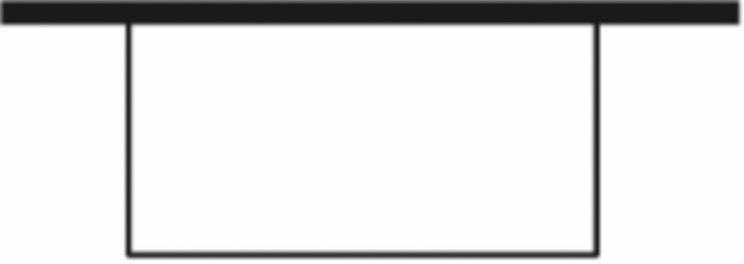
\includegraphics[width=0.28\textwidth]{figures/gao92_q8_fence.png}
\end{center}

\ifanswer
\solbegin
\step{设矩形的长为 $x$ 米，宽为 $y$，则 $xy=18$，}
\step{需要用栅栏长为 $x+2y\geqslant2\sqrt{2xy}=12$，}
\step{当且仅当 $x=2y$，即 $y=3$，$x=6$ 时取等号，故至少需要 $12$ 米栅栏.}
\solend
\fi

\item 已知 $a$ 为正整数，若关于 $x$ 的不等式 $\lvert x-2025\rvert\leqslant a$ 的解集中有且仅有 $7$ 个整数，则 $a$ 的值为\blankline[4.4em].

\ifanswer
\solbegin
\step{不等式 $\lvert x-2025\rvert\leqslant a$，则 $-a\leqslant x-2025\leqslant a$，即 $2025-a\leqslant x\leqslant2025+a$，}
\step{所以不等式 $\lvert x-2025\rvert\leqslant a$ 的解集为 $\{x\mid2025-a\leqslant x\leqslant2025+a\}$，}
\step{若不等式解集中有且仅有 $7$ 个整数，且 $a$ 为正整数，}
\step{由解集的对称性得这 $7$ 个整数以 $2025$ 为中心，向左右两边各延伸 $3$ 个整数，}
\step{即这 $7$ 个整数为 $2022,2023,2024,2025,2026,2027,2028$，所以 $a=3$.}
\solend
\fi

\item 已知关于 $x$ 的一元二次方程 $x^2-x+a=0$ 有两个不相等的正根 $m$、$n$，则 $\dfrac1m+\dfrac9n$ 的最小值为\blankline[4.4em].

\ifanswer
\solbegin
\step{因为一元二次方程 $x^2-x+a=0$ 有两个不相等的正根 $m$、$n$，}
\step{所以判别式 $\Delta=(-1)^2-4a>0\Rightarrow a<\dfrac14$，$m+n=1$，$mn=a>0$，}
\step{因此 $0<a<\dfrac14$ 且 $m+n=1(m,n>0)$.}
\step{$\dfrac1m+\dfrac9n=\left(\dfrac1m+\dfrac9n\right)(m+n)=1+\dfrac nm+\dfrac{9m}{n}+9=10+\dfrac nm+\dfrac{9m}{n}\geqslant10+2\sqrt9=16$，}
\step{等号成立条件为 $\dfrac nm=\dfrac{9m}{n}\Rightarrow n^2=9m^2\Rightarrow n=3m$，}
\step{$m$、$n>0$，结合 $m+n=1$，代入 $n=3m$ 得 $m+3m=1\Rightarrow m=\dfrac14$，$n=\dfrac34$，}
\step{此时 $mn=\dfrac14\cdot\dfrac34=\dfrac3{16}$，满足 $0<a<\dfrac14$，等号可取，因此 $\dfrac1m+\dfrac9n$ 的最小值为 $16$.}
\solend
\fi

\item 对任意 $A$、$B\subseteq R$，记 $A\oplus B=\{x\mid x\in A\cup B,x\notin A\cap B\}$，并称 $A\oplus B$ 为集合 $A$，$B$ 的对称差. 例如：若 $A=\{1,2,3\},B=\{2,3,4\}$，则 $A\oplus B=\{1,4\}$. 下列命题中，为真命题的有\blankline[4.4em].

①若 $A$、$B\subseteq R$ 且 $A\oplus B\subseteq A$，则 $A\subseteq B$

②若 $A$、$B\subseteq R$ 且 $A\oplus B=\varnothing$，则 $A=B$

③若 $A$、$B\subseteq R$ 且 $A\oplus B=B$，则 $A=\varnothing$

④对任意 $A$、$B\subseteq R$，都有 $A\oplus B=\complement_{R}A\oplus\complement_{R}B$

\ifanswer
\solbegin
\step{对于①，因为 $A\oplus B\subseteq A$，所以 $\{x\mid x\in A\cup B,x\notin A\cap B\}\subseteq A$，故 $B\subseteq A$，}
\step{故①错误；}
\step{对于②，$A$、$B\subseteq R$ 且 $A\oplus B=\varnothing$，则 $\varnothing=\{x\mid x\in A\cup B,x\notin A\cap B\}$，}
\step{即 $A\cup B=A\cap B$，所以 $A=B$，故②正确；}
\step{对于③，$A$、$B\subseteq R$ 且 $A\oplus B=B$，则 $B=\{x\mid x\in A\cup B,x\notin A\cap B\}$，}
\step{故 $A\subseteq B$，且 $B$ 中元素不在 $A\cap B$ 中，故 $A=\varnothing$，故③正确；}
\step{对于④，$\complement_{R}A\oplus\complement_{R}B=\{x\mid x\in\complement_{R}A\cup\complement_{R}B,x\notin\complement_{R}A\cap\complement_{R}B\}$，}
\step{其中 $\complement_{R}A\cup\complement_{R}B=\complement_{R}(A\cap B)$，$\complement_{R}A\cap\complement_{R}B=\complement_{R}(A\cup B)$，}
\step{故 $\complement_{R}A\oplus\complement_{R}B=\{x\mid x\in\complement_{R}(A\cap B)$，}
\step{$x\notin\complement_{R}(A\cup B)\}=\{x\mid x\in A\cup B,x\notin A\cap B\}$，}
\step{而 $A\oplus B=\{x\mid x\in A\cup B,x\notin A\cap B\}$，故 $A\oplus B=\complement_{R}A\oplus\complement_{R}B$，故④正确.}
\step{故正确的是②③④.}
\solend
\fi

\item 若不等式 $x^2-2ax+a^2-1\geqslant0$ 对任意 $x\in[0,2]$ 恒成立，则实数 $a$ 的取值范围是\blankline[4.4em].

\ifanswer
\solbegin
\step{由题意不等式 $x^2-2ax+a^2-1\geqslant0$ 对任意 $x\in[0,2]$ 恒成立，}
\step{解得 $x\leqslant a-1$ 或 $x\geqslant a+1$，要使此不等式对任意 $x\in[0,2]$ 恒成立，}
\step{则区间 $[0,2]$ 必须完全包含在解集 $(-\infty,a-1]\cup[a+1,+\infty)$ 中，}
\step{等价于 $[0,2]$ 与开区间 $(a-1,a+1)$ 的交集为空集，}
\step{区间 $[0,2]$ 在 $a-1$ 左侧，即 $2\leqslant a-1$，解得 $a\geqslant3$，}
\step{区间 $[0,2]$ 在 $a+1$ 右侧，即 $a+1\leqslant0$，解得 $a\leqslant-1$，}
\step{当 $a\in(-1,3)$，则 $(a-1,a+1)$ 与 $[0,2]$ 必有交集，不满足条件，}
\step{综上，实数 $a$ 的取值范围是 $(-\infty,-1]\cup[3,+\infty)$.}
\solend
\fi

\end{enumerate}

\bigsec{二、选择题}

\begin{enumerate}
\setcounter{enumi}{12}

\item 若 $a<b<0$，则下列不等式成立的是\mbox{（\quad）}% 原卷括号内已印“D”，试卷版按惯例留空

\keepwithprev
A. $a^2<b^2$\qquad B. $\dfrac1a<\dfrac1b$\qquad C. $ab<b^2$\qquad D. $ab<a^2$

\ifanswer
\ans{$D$}
\fi

\item 已知全集 $U=\{1,2,3,4,5\}$，集合 $A,B$ 是 $U$ 子集，满足 $\overline{A\cup B}=\{4,5\}$，$B=\{2,3\}$，则 $A\cap\overline B=\mbox{（\quad）}$

\keepwithprev
A. $\{1\}$\qquad B. $\{1,2\}$\qquad C. $\{1,4,5\}$\qquad D. $\varnothing$

\ifanswer
\solbegin
\step{因为全集 $U=\{1,2,3,4,5\}$，集合 $A$、$B$ 是 $U$ 子集，$\overline{A\cup B}=\{4,5\}$，$B=\{2,3\}$，}
\step{所以 $A\cup B=\{1,2,3\}$，故 $1\in A$，$1\notin B$，$4\notin A$，$5\notin A$，$4\notin B$，$5\notin B$，}
\step{故 $A\cap\overline B=\{1\}$. 故选 $A$.}
\solend
\fi

\item 设 $a>0$，若关于 $x$ 的不等式 $x^2-(2a-1)x-2a<0$ 的解集中恰有 $3$ 个整数，则实数 $a$ 的取值范围是\mbox{（\quad）}

\keepwithprev
A. $\left[1,\dfrac32\right]$\qquad B. $\left(1,\dfrac32\right]$\qquad C. $\left[\dfrac12,1\right]$\qquad D. $\left(\dfrac12,1\right]$

\ifanswer
\solbegin
\step{已知关于 $x$ 的不等式 $x^2-(2a-1)x-2a<0$，则 $(x+1)(x-2a)<0$，}
\step{则 $-1<x<2a$，又解集中恰有 $3$ 个整数，则 $2<2a\leqslant3$，则 $1<a\leqslant\dfrac32$，}
\step{则 $a$ 的取值范围为 $\left(1,\dfrac32\right]$. 故选 $B$.}
\solend
\fi

\item 已知集合 $U=\{1,2,3,\cdots,2027\}$，$M\subseteq U$，若对于 $M$ 中的任意两个不同的元素 $x$、$y$，都有 $\lvert x-y\rvert>2$，则 $M$ 中元素个数的最大值为\mbox{（\quad）}

\keepwithprev
A. $675$\qquad B. $676$\qquad C. $2025$\qquad D. $2026$

\ifanswer
\solbegin
\step{对于 $M$ 中的任意两个不同的元素 $x$、$y$，都有 $\lvert x-y\rvert>2$，}
\step{不妨设 $x>y$，都有 $x-y\geqslant3$，}
\step{要想 $M$ 所含元素个数最大，则要 $x-y$ 尽可能小，故需使得 $x-y$ 的最小值为 $3$，}
\step{将 $1\sim2027$ 这 $2027$ 个元素按如下分组：}
\step{$\{1,2,3\},\{4,5,6\},\cdots,\{2023,2024,2025\},\{2026,2027\}$，}
\step{故应在前 $675$ 组中按周期 $3$ 每组取一个元素，且第一组中不能取 $3$，}
\step{第一组中取 $1$ 时，得 $M=\{1,4,7,\cdots,2023,2026\}$}
\step{或 $M=\{1,4,7,\cdots,2023,2027\}$ 这样的集合，}
\step{第一组取 $2$ 时，得 $M=\{2,5,8,\cdots,2024,2027\}$，}
\step{其中任意两元素差值 $x-y(x>y)$ 都大于 $2$，满足题意，}
\step{故 $M$ 所含元素个数的最大值为 $\dfrac{2025}{3}+1=676$. 故选 $B$.}
\solend
\fi

\end{enumerate}

\bigsec{三、解答题}

\begin{enumerate}
\setcounter{enumi}{16}

\item 已知集合 $M=\{x\mid a-1\leqslant x\leqslant2a+3\}$，$P=\{x\mid-2<x\leqslant4\}$，全集 $U=R$.

（1）当 $a=2$ 时，求 $M\cap P$；

（2）若 $x\in P$ 是 $x\in M$ 的必要不充分条件，求实数 $a$ 的取值范围.

\ansspace*[9]

\ifanswer
\solbegin
\stepm{（1）}{当 $a=2$ 时，集合 $M=\{x\mid1\leqslant x\leqslant7\}$，所以 $M\cap P=\{x\mid1\leqslant x\leqslant4\}$；}
\stepm{（2）}{因为 $x\in P$ 是 $x\in M$ 的必要不充分条件，所以 $M\subsetneqq P$，}
\step{当 $M=\varnothing$ 时，$a-1>2a+3$，解得 $a<-4$，}
\step{当 $M\neq\varnothing$ 时，则 $\begin{cases}a-1\leqslant2a+3\\ a-1>-2\\ 2a+3\leqslant4\end{cases}$，解得 $-1<a\leqslant\dfrac12$，}
\step{综上所述，实数 $a$ 的取值范围为 $(-\infty,-4)\cup\left(-1,\dfrac12\right]$.}
\solend
\fi

\item 命题甲：关于 $x$ 的方程 $(a-1)x^2+(2a-4)x+a=0$ 有两个不相等的实数根；

命题乙：关于 $x$ 的不等式 $ax^2-2ax+a+1>0$ 的解集为 $R$.

（1）若命题甲为真命题，求实数 $a$ 的取值范围；

（2）若命题甲、乙中至多有一个为真命题，求实数 $a$ 的取值范围.

\ansspace*[12]

\ifanswer
\solbegin
\stepm{（1）}{命题甲：关于 $x$ 的方程 $(a-1)x^2+(2a-4)x+a=0$ 有两个不相等的实数根，}
\step{则 $\begin{cases}a-1\neq0\\ \Delta=(2a-4)^2-4a(a-1)>0\end{cases}$，解得 $a<\dfrac43$ 且 $a\neq1$，}
\step{故 $a$ 的范围为 $\left\{a\left|a<\dfrac43\ \text{且}\ a\neq1\right.\right\}$；}
\stepm{（2）}{当 $a=0$ 时 $y=1>0$，符合题意；}
\step{当 $a\neq0$，由 $\begin{cases}a>0\\ \Delta=4a^2-4a(a+1)<0\end{cases}$，解得 $a>0$，}
\step{则 $a$ 的取值范围为 $a\geqslant0$，}
\step{故 $p$、$q$ 都为真时，$a$ 的范围为 $0\leqslant a<\dfrac43$ 且 $a\neq1$，}
\step{则命题甲、乙中至多有一个为真命题时，}
\step{$a$ 的取值范围为 $\left\{a\left|a<0\ \text{或}\ a=1\ \text{或}\ a\geqslant\dfrac43\right.\right\}$.}
\solend
\fi

\item 如图，$OA$、$OB$ 是两条长度足够长的互相垂直的笔直小路，矩形 $OCPD$ 的顶点 $C$，$D$ 分别在 $OA$、$OB$ 上，且该矩形区域内种满了荷花. 为了让观赏者有更好的观赏体验，现计划经过点 $P$ 修一条小路 $EF$，其中点 $E$ 在小路 $OA$ 上，点 $F$ 在小路 $OB$ 上，并在 $\triangle OEF$ 区域内种满荷花. 已知 $OD=25$ m，$OC=40$ m，且小路 $EF$ 要完全位于一个以 $O$ 为顶点的，边长为 $100$ m 的正方形内部（包括边界）. 记 $\triangle OEF$ 的面积为 $S$ m$^2$.

\begin{center}
\begin{tikzpicture}[x=0.46cm,y=0.42cm,line width=0.7pt]
\draw (0,0) -- (0,10.2) node[above,inner sep=3pt] {$A$};
\draw (0,0) -- (11.8,0) node[right,inner sep=3pt] {$B$};
\draw (0,4.83) -- (2.42,4.83) -- (2.42,0);
\draw (0,6.92) -- (8.01,0);
\node[below left,inner sep=2pt] at (0,0) {$O$};
\node[below,inner sep=2pt] at (2.42,0) {$D$};
\node[left,inner sep=3pt] at (0,4.83) {$C$};
\node[above right,inner sep=1pt] at (2.42,4.83) {$P$};
\node[left,inner sep=3pt] at (0,6.92) {$E$};
\node[below,inner sep=2pt] at (8.01,0) {$F$};
\end{tikzpicture}
\end{center}

（1）设 $EC=x\cdot m$，试用 $x$ 表示 $OF$，并求 $x$ 的取值范围.

（2）当 $EC$ 的长度为多少时，$S$ 取得最小值？最小值是多少？

\ansspace*[11]

\ifanswer
\solbegin
\stepm{（1）}{由题意得 $x\leqslant60$，}
\step{$\triangle PCE\backsim\triangle FDP$，所以 $\dfrac{EC}{CP}=\dfrac{PD}{DF}$，即 $\dfrac{x}{25}=\dfrac{40}{DF}$，得 $DF=\dfrac{1000}{x}$ m，}
\step{所以 $OF=OD+DF=\left(25+\dfrac{1000}{x}\right)$ m，}
\step{所以 $25+\dfrac{1000}{x}\leqslant100$，解得 $x\geqslant\dfrac{40}{3}$；}
\step{综上，$\dfrac{40}{3}\leqslant x\leqslant60$；}
\stepm{（2）}{由 $OE=OC+CE=(40+x)$ m，}
\step{所以 $S=\dfrac12\cdot OF\cdot OE=\dfrac12\left(25+\dfrac{1000}{x}\right)(40+x)$}
\step{$=\dfrac12\left(1000+25x+\dfrac{40000}{x}+1000\right)$ m$^2$，}
\step{由基本不等式得 $S\geqslant\dfrac12\left(2000+2\sqrt{25x\cdot\dfrac{40000}{x}}\right)=2000$ m$^2$，}
\step{当且仅当 $25x=\dfrac{40000}{x}$，即 $x=40$ 时取等号，}
\step{故 $EC=40$ m 时，$S$ 取得最小值，为 $2000$ m$^2$.}
\solend
\fi

\item 已知函数 $f(x)=x^2-(a-2)x+a-3$.

（1）若 $f(x)=0$ 的两根为 $\alpha,\beta$，$\alpha^2+\beta^2=2$，求 $a$ 的值；

（2）解关于 $x$ 的不等式 $f(x)\geqslant0$；

（3）是否存在整数 $m,n$，使得关于 $x$ 的不等式 $m\leqslant f(x)\leqslant n$ 的解集恰好为 $[m,n]$？若存在，求出 $m,n$ 的值. 若不存在，请说明理由.

\ansspace*[16]

\ifanswer
\solbegin
\stepm{（1）}{由韦达定理，$\alpha+\beta=a-2,\alpha\beta=a-3$，}
\step{因此 $\alpha^2+\beta^2=(a-2)^2-2(a-3)=2\Leftrightarrow(a-2)(a-4)=0$，}
\step{$a=2$ 时两根为 $1,-1$；$a=4$ 时两根均为 $1$，均满足条件，}
\step{所以 $a=2$ 或 $a=4$.}
\stepm{（2）}{因为 $f(x)=(x-1)[x-(a-3)]$，所以分三种情况：}
\step{当 $a<4$ 时，$a-3<1$，解集为 $(-\infty,a-3]\cup[1,+\infty)$.}
\step{当 $a=4$ 时，$f(x)=(x-1)^2\geqslant0$ 恒成立，解集为 $R$.}
\step{当 $a>4$ 时，$a-3>1$，解集为 $(-\infty,1]\cup[a-3,+\infty)$.}
\stepm{（3）}{区间 $[m,n]$ 要求 $m<n$. 记 $f(x)$ 的最小值为 $k$.}
\step{$[m,n]$ 非空，不等式 $f(x)\leqslant n$ 有解，其解集为闭区间 $[x_1,x_2]$，}
\step{其中 $x_1\leqslant x_2$ 是方程 $f(x)=n$ 的两根.}
\step{若 $k<m$，则 $f(x)<m$ 的解集是 $[x_1,x_2]$ 内部的一个开区间，}
\step{从 $[x_1,x_2]$ 中去掉它后剩下两段，原不等式的解集不是一个区间，矛盾，}
\step{所以 $k\geqslant m$，原不等式的解集就是 $[x_1,x_2]$，于是 $m=x_1,n=x_2$，}
\step{即 $f(m)=f(n)=n$，于是 $f(m)-f(n)=(m-n)(m+n-a+2)=0$.}
\step{因为 $m\neq n$，所以 $a=m+n+2$.}
\step{代入 $f(m)=n$，得 $(m-1)(1-n)=n\Leftrightarrow m(n-1)=-1$，$m,n$ 均为整数，}
\step{因此 $(m,n)=(-1,2)$ 或 $(m,n)=(1,0)$.}
\step{结合 $m<n$，只可能有 $m=-1,n=2$，此时 $a=3$.}
\step{检验：此时 $f(x)=x^2-x$，且 $x^2-x=\left(x-\dfrac12\right)^2-\dfrac14\geqslant-\dfrac14>-1$，}
\step{因此 $-1\leqslant f(x)\leqslant2\Leftrightarrow x^2-x\leqslant2\Leftrightarrow(x+1)(x-2)\leqslant0\Leftrightarrow x\in[-1,2]$，}
\step{所以存在符合条件的整数 $m=-1,n=2$.}
\solend
\fi

\item 给定数集 $M$，若对于任意 $a$、$b\in M$，有 $a+b\in M,a-b\in M$，则称集合 $M$ 为闭集合.

（1）判断集合 $A_1=\{-4,-2,0,2,4\}$，集合 $B=\{x\mid x=3k,k\in\Z\}$ 是否为闭集合；

（2）若集合 $C$、$D$ 为闭集合，则 $C\cup D$ 是否一定为闭集合？请说明理由；

（3）已知集合 $C$、$D$ 为闭集合，且 $C\subsetneq R,D\subsetneq R$，证明：$(C\cup D)\subsetneq R$.% 原卷印作 (C∪D)⊂R，按解析证明的是 C∪D≠R，排真子集

\ansspace*[14]

\ifanswer
\solbegin
\stepm{（1）}{因为 $4\in A_1$，$2\in A_1$，$4+2=6\notin A_1$，所以 $A_1$ 不是闭集合；}
\step{任取 $x,y\in B$，设 $x=3m,y=3n,m,n\in\Z$，}
\step{则 $x+y=3m+3n=3(m+n)$ 且 $m+n\in\Z$，}
\step{所以 $x+y\in B$，同理，$x-y\in B$，故 $B$ 为闭集合.}
\stepm{（2）}{结论：不一定.}
\step{不妨令 $C=\{x\mid x=2k,k\in\Z\},D=\{x\mid x=3k,k\in\Z\}$，}
\step{则由（1）得 $C$、$D$ 为闭集合，易得 $2,3\in C\cup D,2+3=5\notin C\cup D$，}
\step{因此，$C\cup D$ 不一定是闭集合.}
\stepm{（3）}{不妨假设 $C\cup D=R$，则由 $C\subsetneq R$，得存在 $a\in R$ 且 $a\notin C$，故 $a\in D$.}
\step{同理，存在 $b\in R$ 且 $b\notin D$，故 $b\in C$.}
\step{因为 $a+b\in R=C\cup D$，所以 $a+b\in C$ 或 $a+b\in D$.}
\step{若 $a+b\in C$，则由 $C$ 为闭集合且 $b\in C$，得 $a=(a+b)-b\in C$，}
\step{与 $a\notin C$ 矛盾.}
\step{若 $a+b\in D$，则由 $D$ 为闭集合且 $a\in D$，得 $b=(a+b)-a\in D$，}
\step{与 $b\notin D$ 矛盾.}
\step{综上，$C\cup D=R$ 不成立，故 $(C\cup D)\subsetneq R$.}
\solend
\fi

\end{enumerate}

\end{document}
"
% 紧凑版：xelatex "\def\iscompact{1}% 高一92_闵行实验_10月月考.tex
%   —— 高一上数学“2026-2027 年闵行实验高一上 10 月月考”（讲评版）
% 试卷版：xelatex 高一92_闵行实验_10月月考.tex
% 答案版：xelatex "\def\isanswer{1}% 高一92_闵行实验_10月月考.tex
%   —— 高一上数学“2026-2027 年闵行实验高一上 10 月月考”（讲评版）
% 试卷版：xelatex 高一92_闵行实验_10月月考.tex
% 答案版：xelatex "\def\isanswer{1}\input{高一92_闵行实验_10月月考.tex}"
% 紧凑版：xelatex "\def\iscompact{1}\input{高一92_闵行实验_10月月考.tex}"
%
% 原始材料：微信公众号“魔都数学加油站”文章，连载“27学年高一92”；
% 原文标题“27学年高一92——2026-2027年上海市闵行实验高一上10月月考”；
% 原文链接：https://mp.weixin.qq.com/s/8HUyr3G7GpcHyczwu_XYCQ。
% 正文为 10 张 PNG 页（`原图/高一92_闵行实验_10月月考/01..10.png`），均 4762×6735，按页序读取。
%
% 篇幅与题号：原卷自第 3 题起编号（第 1、2 题不在原文内）。填空题 3—12（10 题）、
% 选择题 13—16（4 题）、解答题 17—21（5 题），共 19 题。
%
% 讲评版：第 6 题只印【答案】（“$[-1,3]$”），本稿只给 \ans{}；第 13 题无【解析】、
% 答案“D”直接印在题干括号内，本稿试卷版按惯例留空、答案版提 \ans{$D$}；其余 17 题印
% 【解析】，其中选择题答案在解析末句“故选 $A$／$B$／$B$”。
% 第 8 题题干右侧有一幅“围墙 + 三面栅栏”示意图（裁自第 2 页原图）；第 19 题题干带
% 与 高一88 第 19 题同型的示意图（$OA$／$OB$ 两条小路、矩形 $OCPD$、折线 $EF$），用 TikZ 重绘。
%
% 副标题：原卷未印副标题。本稿按内容标作“集合与常用逻辑用语、不等式”。
%
% 原卷笔误/存疑（均照录未改，正文对应处另有 % 注）：
%   ① 第 21 题 (3) 题干与解析末句把结论印作“$(C\cup D)\subset R$”，而解析证明的是
%      “$C\cup D=\R$ 不成立”，按文意应为“$(C\cup D)\subsetneq\R$”；本稿按真子集排
%      $\subsetneq$，原卷记号照录于文件头；
%   ② 第 7 题解析只列 $B=\varnothing$（$a=0$）、$B=\{1\}$（$a=1$）、$B=\{-3\}$（$a=-\frac13$）
%      三种情形，与结论 $\left\{0,1,-\frac13\right\}$ 相符，无笔误。
%
% 与原卷的排版差异：
%   ① 原卷每题下直接印【答案】/【解析】，本稿按全稿惯例将答案与解析置于答案版；
%   ② 原卷未印副标题，本稿补出；填空横线统一排 \blankline[4.4em]；
%   ③ 原卷数集记号排斜体 $R$、$Z$，本稿按全稿惯例改用 $\R$、$\Z$；
%   ④ 第 17—21 题的子问用行内“（1）（2）（3）”段，解析中的子问标号用 \stepm；
%   ⑤ 解答题按惯例加 \ansspace；选择题括号排 \mbox{（\quad）}；
%   ⑥ 第 8 题的示意图原卷排在题干右侧、文字绕排，本稿改排为题干后的居中图
%      （自原图裁切、去粉色水印后转灰度）；第 19 题的图按原图比例 TikZ 重绘。
%
% 行数核对：逐题数 \step/\stepm 条数，合计 128 条（Q3：2；Q4：3；Q5：2；Q6：0；Q7：6；
% Q8：3；Q9：5；Q10：7；Q11：12；Q12：8；Q13：0；Q14：3；Q15：3；Q16：11；Q17：5；
% Q18：9；Q19：11；Q20：22；Q21：16）。第 6 题只印答案、第 13 题无解析，均不计入 \step 账。
% 原卷解析的换行按语意合并，未逐行强拆。
%
\documentclass[a4paper,11pt]{article}
\usepackage{common}

\begin{document}

\examtitlest[7]{2026--2027 年闵行实验高一上 10 月月考}{集合与常用逻辑用语、不等式}

\bigsec{一、填空题}

\begin{enumerate}
\setcounter{enumi}{2}

\item 已知 $3<a<8$，$4<b<9$，则 $\dfrac ab$ 的取值范围是\blankline[4.4em].

\ifanswer
\solbegin
\step{因为 $4<b<9$，所以 $\dfrac19<\dfrac1b<\dfrac14$，又 $3<a<8$，所以 $\dfrac13<\dfrac ab<2$，}
\step{故 $\dfrac ab$ 的取值范围是 $\left(\dfrac13,2\right)$.}
\solend
\fi

\item 已知 $p:x>3$，$q:x>5$，则 $p$ 是 $q$ 的\blankline[4.4em]（选“充分不必要条件”“必要不充分条件”“充要条件”“既不充分也不必要条件”之一填空）.

\ifanswer
\solbegin
\step{当 $x>3$ 时，不能推出 $x>5$，充分性不成立；}
\step{当 $x>5$ 时，可以得到 $x>3$，必要性成立；}
\step{故 $p$ 是 $q$ 的必要不充分条件.}
\solend
\fi

\item 不等式 $\dfrac{x-1}{2x+1}\leqslant1$ 的解集为\blankline[4.4em].

\ifanswer
\solbegin
\step{因为 $\dfrac{x-1}{2x+1}\leqslant1$，所以 $\dfrac{x-1}{2x+1}-\dfrac{2x+1}{2x+1}\leqslant0$，所以 $\dfrac{x+2}{2x+1}\geqslant0$，}
\step{所以 $x>-\dfrac12$ 或 $x\leqslant-2$，即不等式的解集是 $(-\infty,-2]\cup\left(-\dfrac12,+\infty\right)$.}
\solend
\fi

\item 设 $x\in R$，则方程 $\lvert x+1\rvert+\lvert x-3\rvert=4$ 的解集为\blankline[4.4em].

\ifanswer
\ans{$[-1,3]$}
\fi

\item 若 $A=\{x\mid x^2+2x=3\}$，$B=\{x\mid ax=1\}$，且 $B\subseteq A$，则实数 $a$ 的值组成的集合为\blankline[4.4em].

\ifanswer
\solbegin
\step{由 $x^2+2x=3$ 得 $x^2+2x-3=0$，解得 $x=1$ 或 $x=-3$，所以 $A=\{1,-3\}$，}
\step{又因为 $B=\{x\mid ax=1\}$，且 $B\subseteq A$，}
\step{当 $B=\varnothing$，即 $a=0$ 时，显然符合题意；}
\step{当 $B=\{1\}$，即 $a=1$ 时，也符合题意；}
\step{当 $B=\{-3\}$，即 $a=-\dfrac13$ 时，也符合题意；}
\step{综上所述，实数 $a$ 的值组成的集合为 $\left\{0,1,-\dfrac13\right\}$.}
\solend
\fi

\item 某校欲在围墙边用栅栏围成一个 $18$ 平方米的矩形区域，作为天鹅的地面栖息地，矩形区域的一条边为围墙（如图），则至少需要\blankline[4.4em]米栅栏.

\begin{center}
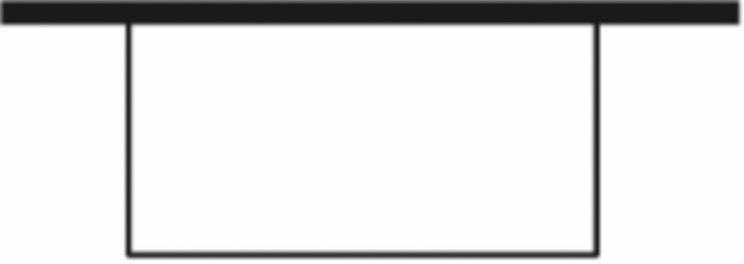
\includegraphics[width=0.28\textwidth]{figures/gao92_q8_fence.png}
\end{center}

\ifanswer
\solbegin
\step{设矩形的长为 $x$ 米，宽为 $y$，则 $xy=18$，}
\step{需要用栅栏长为 $x+2y\geqslant2\sqrt{2xy}=12$，}
\step{当且仅当 $x=2y$，即 $y=3$，$x=6$ 时取等号，故至少需要 $12$ 米栅栏.}
\solend
\fi

\item 已知 $a$ 为正整数，若关于 $x$ 的不等式 $\lvert x-2025\rvert\leqslant a$ 的解集中有且仅有 $7$ 个整数，则 $a$ 的值为\blankline[4.4em].

\ifanswer
\solbegin
\step{不等式 $\lvert x-2025\rvert\leqslant a$，则 $-a\leqslant x-2025\leqslant a$，即 $2025-a\leqslant x\leqslant2025+a$，}
\step{所以不等式 $\lvert x-2025\rvert\leqslant a$ 的解集为 $\{x\mid2025-a\leqslant x\leqslant2025+a\}$，}
\step{若不等式解集中有且仅有 $7$ 个整数，且 $a$ 为正整数，}
\step{由解集的对称性得这 $7$ 个整数以 $2025$ 为中心，向左右两边各延伸 $3$ 个整数，}
\step{即这 $7$ 个整数为 $2022,2023,2024,2025,2026,2027,2028$，所以 $a=3$.}
\solend
\fi

\item 已知关于 $x$ 的一元二次方程 $x^2-x+a=0$ 有两个不相等的正根 $m$、$n$，则 $\dfrac1m+\dfrac9n$ 的最小值为\blankline[4.4em].

\ifanswer
\solbegin
\step{因为一元二次方程 $x^2-x+a=0$ 有两个不相等的正根 $m$、$n$，}
\step{所以判别式 $\Delta=(-1)^2-4a>0\Rightarrow a<\dfrac14$，$m+n=1$，$mn=a>0$，}
\step{因此 $0<a<\dfrac14$ 且 $m+n=1(m,n>0)$.}
\step{$\dfrac1m+\dfrac9n=\left(\dfrac1m+\dfrac9n\right)(m+n)=1+\dfrac nm+\dfrac{9m}{n}+9=10+\dfrac nm+\dfrac{9m}{n}\geqslant10+2\sqrt9=16$，}
\step{等号成立条件为 $\dfrac nm=\dfrac{9m}{n}\Rightarrow n^2=9m^2\Rightarrow n=3m$，}
\step{$m$、$n>0$，结合 $m+n=1$，代入 $n=3m$ 得 $m+3m=1\Rightarrow m=\dfrac14$，$n=\dfrac34$，}
\step{此时 $mn=\dfrac14\cdot\dfrac34=\dfrac3{16}$，满足 $0<a<\dfrac14$，等号可取，因此 $\dfrac1m+\dfrac9n$ 的最小值为 $16$.}
\solend
\fi

\item 对任意 $A$、$B\subseteq R$，记 $A\oplus B=\{x\mid x\in A\cup B,x\notin A\cap B\}$，并称 $A\oplus B$ 为集合 $A$，$B$ 的对称差. 例如：若 $A=\{1,2,3\},B=\{2,3,4\}$，则 $A\oplus B=\{1,4\}$. 下列命题中，为真命题的有\blankline[4.4em].

①若 $A$、$B\subseteq R$ 且 $A\oplus B\subseteq A$，则 $A\subseteq B$

②若 $A$、$B\subseteq R$ 且 $A\oplus B=\varnothing$，则 $A=B$

③若 $A$、$B\subseteq R$ 且 $A\oplus B=B$，则 $A=\varnothing$

④对任意 $A$、$B\subseteq R$，都有 $A\oplus B=\complement_{R}A\oplus\complement_{R}B$

\ifanswer
\solbegin
\step{对于①，因为 $A\oplus B\subseteq A$，所以 $\{x\mid x\in A\cup B,x\notin A\cap B\}\subseteq A$，故 $B\subseteq A$，}
\step{故①错误；}
\step{对于②，$A$、$B\subseteq R$ 且 $A\oplus B=\varnothing$，则 $\varnothing=\{x\mid x\in A\cup B,x\notin A\cap B\}$，}
\step{即 $A\cup B=A\cap B$，所以 $A=B$，故②正确；}
\step{对于③，$A$、$B\subseteq R$ 且 $A\oplus B=B$，则 $B=\{x\mid x\in A\cup B,x\notin A\cap B\}$，}
\step{故 $A\subseteq B$，且 $B$ 中元素不在 $A\cap B$ 中，故 $A=\varnothing$，故③正确；}
\step{对于④，$\complement_{R}A\oplus\complement_{R}B=\{x\mid x\in\complement_{R}A\cup\complement_{R}B,x\notin\complement_{R}A\cap\complement_{R}B\}$，}
\step{其中 $\complement_{R}A\cup\complement_{R}B=\complement_{R}(A\cap B)$，$\complement_{R}A\cap\complement_{R}B=\complement_{R}(A\cup B)$，}
\step{故 $\complement_{R}A\oplus\complement_{R}B=\{x\mid x\in\complement_{R}(A\cap B)$，}
\step{$x\notin\complement_{R}(A\cup B)\}=\{x\mid x\in A\cup B,x\notin A\cap B\}$，}
\step{而 $A\oplus B=\{x\mid x\in A\cup B,x\notin A\cap B\}$，故 $A\oplus B=\complement_{R}A\oplus\complement_{R}B$，故④正确.}
\step{故正确的是②③④.}
\solend
\fi

\item 若不等式 $x^2-2ax+a^2-1\geqslant0$ 对任意 $x\in[0,2]$ 恒成立，则实数 $a$ 的取值范围是\blankline[4.4em].

\ifanswer
\solbegin
\step{由题意不等式 $x^2-2ax+a^2-1\geqslant0$ 对任意 $x\in[0,2]$ 恒成立，}
\step{解得 $x\leqslant a-1$ 或 $x\geqslant a+1$，要使此不等式对任意 $x\in[0,2]$ 恒成立，}
\step{则区间 $[0,2]$ 必须完全包含在解集 $(-\infty,a-1]\cup[a+1,+\infty)$ 中，}
\step{等价于 $[0,2]$ 与开区间 $(a-1,a+1)$ 的交集为空集，}
\step{区间 $[0,2]$ 在 $a-1$ 左侧，即 $2\leqslant a-1$，解得 $a\geqslant3$，}
\step{区间 $[0,2]$ 在 $a+1$ 右侧，即 $a+1\leqslant0$，解得 $a\leqslant-1$，}
\step{当 $a\in(-1,3)$，则 $(a-1,a+1)$ 与 $[0,2]$ 必有交集，不满足条件，}
\step{综上，实数 $a$ 的取值范围是 $(-\infty,-1]\cup[3,+\infty)$.}
\solend
\fi

\end{enumerate}

\bigsec{二、选择题}

\begin{enumerate}
\setcounter{enumi}{12}

\item 若 $a<b<0$，则下列不等式成立的是\mbox{（\quad）}% 原卷括号内已印“D”，试卷版按惯例留空

\keepwithprev
A. $a^2<b^2$\qquad B. $\dfrac1a<\dfrac1b$\qquad C. $ab<b^2$\qquad D. $ab<a^2$

\ifanswer
\ans{$D$}
\fi

\item 已知全集 $U=\{1,2,3,4,5\}$，集合 $A,B$ 是 $U$ 子集，满足 $\overline{A\cup B}=\{4,5\}$，$B=\{2,3\}$，则 $A\cap\overline B=\mbox{（\quad）}$

\keepwithprev
A. $\{1\}$\qquad B. $\{1,2\}$\qquad C. $\{1,4,5\}$\qquad D. $\varnothing$

\ifanswer
\solbegin
\step{因为全集 $U=\{1,2,3,4,5\}$，集合 $A$、$B$ 是 $U$ 子集，$\overline{A\cup B}=\{4,5\}$，$B=\{2,3\}$，}
\step{所以 $A\cup B=\{1,2,3\}$，故 $1\in A$，$1\notin B$，$4\notin A$，$5\notin A$，$4\notin B$，$5\notin B$，}
\step{故 $A\cap\overline B=\{1\}$. 故选 $A$.}
\solend
\fi

\item 设 $a>0$，若关于 $x$ 的不等式 $x^2-(2a-1)x-2a<0$ 的解集中恰有 $3$ 个整数，则实数 $a$ 的取值范围是\mbox{（\quad）}

\keepwithprev
A. $\left[1,\dfrac32\right]$\qquad B. $\left(1,\dfrac32\right]$\qquad C. $\left[\dfrac12,1\right]$\qquad D. $\left(\dfrac12,1\right]$

\ifanswer
\solbegin
\step{已知关于 $x$ 的不等式 $x^2-(2a-1)x-2a<0$，则 $(x+1)(x-2a)<0$，}
\step{则 $-1<x<2a$，又解集中恰有 $3$ 个整数，则 $2<2a\leqslant3$，则 $1<a\leqslant\dfrac32$，}
\step{则 $a$ 的取值范围为 $\left(1,\dfrac32\right]$. 故选 $B$.}
\solend
\fi

\item 已知集合 $U=\{1,2,3,\cdots,2027\}$，$M\subseteq U$，若对于 $M$ 中的任意两个不同的元素 $x$、$y$，都有 $\lvert x-y\rvert>2$，则 $M$ 中元素个数的最大值为\mbox{（\quad）}

\keepwithprev
A. $675$\qquad B. $676$\qquad C. $2025$\qquad D. $2026$

\ifanswer
\solbegin
\step{对于 $M$ 中的任意两个不同的元素 $x$、$y$，都有 $\lvert x-y\rvert>2$，}
\step{不妨设 $x>y$，都有 $x-y\geqslant3$，}
\step{要想 $M$ 所含元素个数最大，则要 $x-y$ 尽可能小，故需使得 $x-y$ 的最小值为 $3$，}
\step{将 $1\sim2027$ 这 $2027$ 个元素按如下分组：}
\step{$\{1,2,3\},\{4,5,6\},\cdots,\{2023,2024,2025\},\{2026,2027\}$，}
\step{故应在前 $675$ 组中按周期 $3$ 每组取一个元素，且第一组中不能取 $3$，}
\step{第一组中取 $1$ 时，得 $M=\{1,4,7,\cdots,2023,2026\}$}
\step{或 $M=\{1,4,7,\cdots,2023,2027\}$ 这样的集合，}
\step{第一组取 $2$ 时，得 $M=\{2,5,8,\cdots,2024,2027\}$，}
\step{其中任意两元素差值 $x-y(x>y)$ 都大于 $2$，满足题意，}
\step{故 $M$ 所含元素个数的最大值为 $\dfrac{2025}{3}+1=676$. 故选 $B$.}
\solend
\fi

\end{enumerate}

\bigsec{三、解答题}

\begin{enumerate}
\setcounter{enumi}{16}

\item 已知集合 $M=\{x\mid a-1\leqslant x\leqslant2a+3\}$，$P=\{x\mid-2<x\leqslant4\}$，全集 $U=R$.

（1）当 $a=2$ 时，求 $M\cap P$；

（2）若 $x\in P$ 是 $x\in M$ 的必要不充分条件，求实数 $a$ 的取值范围.

\ansspace*[9]

\ifanswer
\solbegin
\stepm{（1）}{当 $a=2$ 时，集合 $M=\{x\mid1\leqslant x\leqslant7\}$，所以 $M\cap P=\{x\mid1\leqslant x\leqslant4\}$；}
\stepm{（2）}{因为 $x\in P$ 是 $x\in M$ 的必要不充分条件，所以 $M\subsetneqq P$，}
\step{当 $M=\varnothing$ 时，$a-1>2a+3$，解得 $a<-4$，}
\step{当 $M\neq\varnothing$ 时，则 $\begin{cases}a-1\leqslant2a+3\\ a-1>-2\\ 2a+3\leqslant4\end{cases}$，解得 $-1<a\leqslant\dfrac12$，}
\step{综上所述，实数 $a$ 的取值范围为 $(-\infty,-4)\cup\left(-1,\dfrac12\right]$.}
\solend
\fi

\item 命题甲：关于 $x$ 的方程 $(a-1)x^2+(2a-4)x+a=0$ 有两个不相等的实数根；

命题乙：关于 $x$ 的不等式 $ax^2-2ax+a+1>0$ 的解集为 $R$.

（1）若命题甲为真命题，求实数 $a$ 的取值范围；

（2）若命题甲、乙中至多有一个为真命题，求实数 $a$ 的取值范围.

\ansspace*[12]

\ifanswer
\solbegin
\stepm{（1）}{命题甲：关于 $x$ 的方程 $(a-1)x^2+(2a-4)x+a=0$ 有两个不相等的实数根，}
\step{则 $\begin{cases}a-1\neq0\\ \Delta=(2a-4)^2-4a(a-1)>0\end{cases}$，解得 $a<\dfrac43$ 且 $a\neq1$，}
\step{故 $a$ 的范围为 $\left\{a\left|a<\dfrac43\ \text{且}\ a\neq1\right.\right\}$；}
\stepm{（2）}{当 $a=0$ 时 $y=1>0$，符合题意；}
\step{当 $a\neq0$，由 $\begin{cases}a>0\\ \Delta=4a^2-4a(a+1)<0\end{cases}$，解得 $a>0$，}
\step{则 $a$ 的取值范围为 $a\geqslant0$，}
\step{故 $p$、$q$ 都为真时，$a$ 的范围为 $0\leqslant a<\dfrac43$ 且 $a\neq1$，}
\step{则命题甲、乙中至多有一个为真命题时，}
\step{$a$ 的取值范围为 $\left\{a\left|a<0\ \text{或}\ a=1\ \text{或}\ a\geqslant\dfrac43\right.\right\}$.}
\solend
\fi

\item 如图，$OA$、$OB$ 是两条长度足够长的互相垂直的笔直小路，矩形 $OCPD$ 的顶点 $C$，$D$ 分别在 $OA$、$OB$ 上，且该矩形区域内种满了荷花. 为了让观赏者有更好的观赏体验，现计划经过点 $P$ 修一条小路 $EF$，其中点 $E$ 在小路 $OA$ 上，点 $F$ 在小路 $OB$ 上，并在 $\triangle OEF$ 区域内种满荷花. 已知 $OD=25$ m，$OC=40$ m，且小路 $EF$ 要完全位于一个以 $O$ 为顶点的，边长为 $100$ m 的正方形内部（包括边界）. 记 $\triangle OEF$ 的面积为 $S$ m$^2$.

\begin{center}
\begin{tikzpicture}[x=0.46cm,y=0.42cm,line width=0.7pt]
\draw (0,0) -- (0,10.2) node[above,inner sep=3pt] {$A$};
\draw (0,0) -- (11.8,0) node[right,inner sep=3pt] {$B$};
\draw (0,4.83) -- (2.42,4.83) -- (2.42,0);
\draw (0,6.92) -- (8.01,0);
\node[below left,inner sep=2pt] at (0,0) {$O$};
\node[below,inner sep=2pt] at (2.42,0) {$D$};
\node[left,inner sep=3pt] at (0,4.83) {$C$};
\node[above right,inner sep=1pt] at (2.42,4.83) {$P$};
\node[left,inner sep=3pt] at (0,6.92) {$E$};
\node[below,inner sep=2pt] at (8.01,0) {$F$};
\end{tikzpicture}
\end{center}

（1）设 $EC=x\cdot m$，试用 $x$ 表示 $OF$，并求 $x$ 的取值范围.

（2）当 $EC$ 的长度为多少时，$S$ 取得最小值？最小值是多少？

\ansspace*[11]

\ifanswer
\solbegin
\stepm{（1）}{由题意得 $x\leqslant60$，}
\step{$\triangle PCE\backsim\triangle FDP$，所以 $\dfrac{EC}{CP}=\dfrac{PD}{DF}$，即 $\dfrac{x}{25}=\dfrac{40}{DF}$，得 $DF=\dfrac{1000}{x}$ m，}
\step{所以 $OF=OD+DF=\left(25+\dfrac{1000}{x}\right)$ m，}
\step{所以 $25+\dfrac{1000}{x}\leqslant100$，解得 $x\geqslant\dfrac{40}{3}$；}
\step{综上，$\dfrac{40}{3}\leqslant x\leqslant60$；}
\stepm{（2）}{由 $OE=OC+CE=(40+x)$ m，}
\step{所以 $S=\dfrac12\cdot OF\cdot OE=\dfrac12\left(25+\dfrac{1000}{x}\right)(40+x)$}
\step{$=\dfrac12\left(1000+25x+\dfrac{40000}{x}+1000\right)$ m$^2$，}
\step{由基本不等式得 $S\geqslant\dfrac12\left(2000+2\sqrt{25x\cdot\dfrac{40000}{x}}\right)=2000$ m$^2$，}
\step{当且仅当 $25x=\dfrac{40000}{x}$，即 $x=40$ 时取等号，}
\step{故 $EC=40$ m 时，$S$ 取得最小值，为 $2000$ m$^2$.}
\solend
\fi

\item 已知函数 $f(x)=x^2-(a-2)x+a-3$.

（1）若 $f(x)=0$ 的两根为 $\alpha,\beta$，$\alpha^2+\beta^2=2$，求 $a$ 的值；

（2）解关于 $x$ 的不等式 $f(x)\geqslant0$；

（3）是否存在整数 $m,n$，使得关于 $x$ 的不等式 $m\leqslant f(x)\leqslant n$ 的解集恰好为 $[m,n]$？若存在，求出 $m,n$ 的值. 若不存在，请说明理由.

\ansspace*[16]

\ifanswer
\solbegin
\stepm{（1）}{由韦达定理，$\alpha+\beta=a-2,\alpha\beta=a-3$，}
\step{因此 $\alpha^2+\beta^2=(a-2)^2-2(a-3)=2\Leftrightarrow(a-2)(a-4)=0$，}
\step{$a=2$ 时两根为 $1,-1$；$a=4$ 时两根均为 $1$，均满足条件，}
\step{所以 $a=2$ 或 $a=4$.}
\stepm{（2）}{因为 $f(x)=(x-1)[x-(a-3)]$，所以分三种情况：}
\step{当 $a<4$ 时，$a-3<1$，解集为 $(-\infty,a-3]\cup[1,+\infty)$.}
\step{当 $a=4$ 时，$f(x)=(x-1)^2\geqslant0$ 恒成立，解集为 $R$.}
\step{当 $a>4$ 时，$a-3>1$，解集为 $(-\infty,1]\cup[a-3,+\infty)$.}
\stepm{（3）}{区间 $[m,n]$ 要求 $m<n$. 记 $f(x)$ 的最小值为 $k$.}
\step{$[m,n]$ 非空，不等式 $f(x)\leqslant n$ 有解，其解集为闭区间 $[x_1,x_2]$，}
\step{其中 $x_1\leqslant x_2$ 是方程 $f(x)=n$ 的两根.}
\step{若 $k<m$，则 $f(x)<m$ 的解集是 $[x_1,x_2]$ 内部的一个开区间，}
\step{从 $[x_1,x_2]$ 中去掉它后剩下两段，原不等式的解集不是一个区间，矛盾，}
\step{所以 $k\geqslant m$，原不等式的解集就是 $[x_1,x_2]$，于是 $m=x_1,n=x_2$，}
\step{即 $f(m)=f(n)=n$，于是 $f(m)-f(n)=(m-n)(m+n-a+2)=0$.}
\step{因为 $m\neq n$，所以 $a=m+n+2$.}
\step{代入 $f(m)=n$，得 $(m-1)(1-n)=n\Leftrightarrow m(n-1)=-1$，$m,n$ 均为整数，}
\step{因此 $(m,n)=(-1,2)$ 或 $(m,n)=(1,0)$.}
\step{结合 $m<n$，只可能有 $m=-1,n=2$，此时 $a=3$.}
\step{检验：此时 $f(x)=x^2-x$，且 $x^2-x=\left(x-\dfrac12\right)^2-\dfrac14\geqslant-\dfrac14>-1$，}
\step{因此 $-1\leqslant f(x)\leqslant2\Leftrightarrow x^2-x\leqslant2\Leftrightarrow(x+1)(x-2)\leqslant0\Leftrightarrow x\in[-1,2]$，}
\step{所以存在符合条件的整数 $m=-1,n=2$.}
\solend
\fi

\item 给定数集 $M$，若对于任意 $a$、$b\in M$，有 $a+b\in M,a-b\in M$，则称集合 $M$ 为闭集合.

（1）判断集合 $A_1=\{-4,-2,0,2,4\}$，集合 $B=\{x\mid x=3k,k\in\Z\}$ 是否为闭集合；

（2）若集合 $C$、$D$ 为闭集合，则 $C\cup D$ 是否一定为闭集合？请说明理由；

（3）已知集合 $C$、$D$ 为闭集合，且 $C\subsetneq R,D\subsetneq R$，证明：$(C\cup D)\subsetneq R$.% 原卷印作 (C∪D)⊂R，按解析证明的是 C∪D≠R，排真子集

\ansspace*[14]

\ifanswer
\solbegin
\stepm{（1）}{因为 $4\in A_1$，$2\in A_1$，$4+2=6\notin A_1$，所以 $A_1$ 不是闭集合；}
\step{任取 $x,y\in B$，设 $x=3m,y=3n,m,n\in\Z$，}
\step{则 $x+y=3m+3n=3(m+n)$ 且 $m+n\in\Z$，}
\step{所以 $x+y\in B$，同理，$x-y\in B$，故 $B$ 为闭集合.}
\stepm{（2）}{结论：不一定.}
\step{不妨令 $C=\{x\mid x=2k,k\in\Z\},D=\{x\mid x=3k,k\in\Z\}$，}
\step{则由（1）得 $C$、$D$ 为闭集合，易得 $2,3\in C\cup D,2+3=5\notin C\cup D$，}
\step{因此，$C\cup D$ 不一定是闭集合.}
\stepm{（3）}{不妨假设 $C\cup D=R$，则由 $C\subsetneq R$，得存在 $a\in R$ 且 $a\notin C$，故 $a\in D$.}
\step{同理，存在 $b\in R$ 且 $b\notin D$，故 $b\in C$.}
\step{因为 $a+b\in R=C\cup D$，所以 $a+b\in C$ 或 $a+b\in D$.}
\step{若 $a+b\in C$，则由 $C$ 为闭集合且 $b\in C$，得 $a=(a+b)-b\in C$，}
\step{与 $a\notin C$ 矛盾.}
\step{若 $a+b\in D$，则由 $D$ 为闭集合且 $a\in D$，得 $b=(a+b)-a\in D$，}
\step{与 $b\notin D$ 矛盾.}
\step{综上，$C\cup D=R$ 不成立，故 $(C\cup D)\subsetneq R$.}
\solend
\fi

\end{enumerate}

\end{document}
"
% 紧凑版：xelatex "\def\iscompact{1}% 高一92_闵行实验_10月月考.tex
%   —— 高一上数学“2026-2027 年闵行实验高一上 10 月月考”（讲评版）
% 试卷版：xelatex 高一92_闵行实验_10月月考.tex
% 答案版：xelatex "\def\isanswer{1}\input{高一92_闵行实验_10月月考.tex}"
% 紧凑版：xelatex "\def\iscompact{1}\input{高一92_闵行实验_10月月考.tex}"
%
% 原始材料：微信公众号“魔都数学加油站”文章，连载“27学年高一92”；
% 原文标题“27学年高一92——2026-2027年上海市闵行实验高一上10月月考”；
% 原文链接：https://mp.weixin.qq.com/s/8HUyr3G7GpcHyczwu_XYCQ。
% 正文为 10 张 PNG 页（`原图/高一92_闵行实验_10月月考/01..10.png`），均 4762×6735，按页序读取。
%
% 篇幅与题号：原卷自第 3 题起编号（第 1、2 题不在原文内）。填空题 3—12（10 题）、
% 选择题 13—16（4 题）、解答题 17—21（5 题），共 19 题。
%
% 讲评版：第 6 题只印【答案】（“$[-1,3]$”），本稿只给 \ans{}；第 13 题无【解析】、
% 答案“D”直接印在题干括号内，本稿试卷版按惯例留空、答案版提 \ans{$D$}；其余 17 题印
% 【解析】，其中选择题答案在解析末句“故选 $A$／$B$／$B$”。
% 第 8 题题干右侧有一幅“围墙 + 三面栅栏”示意图（裁自第 2 页原图）；第 19 题题干带
% 与 高一88 第 19 题同型的示意图（$OA$／$OB$ 两条小路、矩形 $OCPD$、折线 $EF$），用 TikZ 重绘。
%
% 副标题：原卷未印副标题。本稿按内容标作“集合与常用逻辑用语、不等式”。
%
% 原卷笔误/存疑（均照录未改，正文对应处另有 % 注）：
%   ① 第 21 题 (3) 题干与解析末句把结论印作“$(C\cup D)\subset R$”，而解析证明的是
%      “$C\cup D=\R$ 不成立”，按文意应为“$(C\cup D)\subsetneq\R$”；本稿按真子集排
%      $\subsetneq$，原卷记号照录于文件头；
%   ② 第 7 题解析只列 $B=\varnothing$（$a=0$）、$B=\{1\}$（$a=1$）、$B=\{-3\}$（$a=-\frac13$）
%      三种情形，与结论 $\left\{0,1,-\frac13\right\}$ 相符，无笔误。
%
% 与原卷的排版差异：
%   ① 原卷每题下直接印【答案】/【解析】，本稿按全稿惯例将答案与解析置于答案版；
%   ② 原卷未印副标题，本稿补出；填空横线统一排 \blankline[4.4em]；
%   ③ 原卷数集记号排斜体 $R$、$Z$，本稿按全稿惯例改用 $\R$、$\Z$；
%   ④ 第 17—21 题的子问用行内“（1）（2）（3）”段，解析中的子问标号用 \stepm；
%   ⑤ 解答题按惯例加 \ansspace；选择题括号排 \mbox{（\quad）}；
%   ⑥ 第 8 题的示意图原卷排在题干右侧、文字绕排，本稿改排为题干后的居中图
%      （自原图裁切、去粉色水印后转灰度）；第 19 题的图按原图比例 TikZ 重绘。
%
% 行数核对：逐题数 \step/\stepm 条数，合计 128 条（Q3：2；Q4：3；Q5：2；Q6：0；Q7：6；
% Q8：3；Q9：5；Q10：7；Q11：12；Q12：8；Q13：0；Q14：3；Q15：3；Q16：11；Q17：5；
% Q18：9；Q19：11；Q20：22；Q21：16）。第 6 题只印答案、第 13 题无解析，均不计入 \step 账。
% 原卷解析的换行按语意合并，未逐行强拆。
%
\documentclass[a4paper,11pt]{article}
\usepackage{common}

\begin{document}

\examtitlest[7]{2026--2027 年闵行实验高一上 10 月月考}{集合与常用逻辑用语、不等式}

\bigsec{一、填空题}

\begin{enumerate}
\setcounter{enumi}{2}

\item 已知 $3<a<8$，$4<b<9$，则 $\dfrac ab$ 的取值范围是\blankline[4.4em].

\ifanswer
\solbegin
\step{因为 $4<b<9$，所以 $\dfrac19<\dfrac1b<\dfrac14$，又 $3<a<8$，所以 $\dfrac13<\dfrac ab<2$，}
\step{故 $\dfrac ab$ 的取值范围是 $\left(\dfrac13,2\right)$.}
\solend
\fi

\item 已知 $p:x>3$，$q:x>5$，则 $p$ 是 $q$ 的\blankline[4.4em]（选“充分不必要条件”“必要不充分条件”“充要条件”“既不充分也不必要条件”之一填空）.

\ifanswer
\solbegin
\step{当 $x>3$ 时，不能推出 $x>5$，充分性不成立；}
\step{当 $x>5$ 时，可以得到 $x>3$，必要性成立；}
\step{故 $p$ 是 $q$ 的必要不充分条件.}
\solend
\fi

\item 不等式 $\dfrac{x-1}{2x+1}\leqslant1$ 的解集为\blankline[4.4em].

\ifanswer
\solbegin
\step{因为 $\dfrac{x-1}{2x+1}\leqslant1$，所以 $\dfrac{x-1}{2x+1}-\dfrac{2x+1}{2x+1}\leqslant0$，所以 $\dfrac{x+2}{2x+1}\geqslant0$，}
\step{所以 $x>-\dfrac12$ 或 $x\leqslant-2$，即不等式的解集是 $(-\infty,-2]\cup\left(-\dfrac12,+\infty\right)$.}
\solend
\fi

\item 设 $x\in R$，则方程 $\lvert x+1\rvert+\lvert x-3\rvert=4$ 的解集为\blankline[4.4em].

\ifanswer
\ans{$[-1,3]$}
\fi

\item 若 $A=\{x\mid x^2+2x=3\}$，$B=\{x\mid ax=1\}$，且 $B\subseteq A$，则实数 $a$ 的值组成的集合为\blankline[4.4em].

\ifanswer
\solbegin
\step{由 $x^2+2x=3$ 得 $x^2+2x-3=0$，解得 $x=1$ 或 $x=-3$，所以 $A=\{1,-3\}$，}
\step{又因为 $B=\{x\mid ax=1\}$，且 $B\subseteq A$，}
\step{当 $B=\varnothing$，即 $a=0$ 时，显然符合题意；}
\step{当 $B=\{1\}$，即 $a=1$ 时，也符合题意；}
\step{当 $B=\{-3\}$，即 $a=-\dfrac13$ 时，也符合题意；}
\step{综上所述，实数 $a$ 的值组成的集合为 $\left\{0,1,-\dfrac13\right\}$.}
\solend
\fi

\item 某校欲在围墙边用栅栏围成一个 $18$ 平方米的矩形区域，作为天鹅的地面栖息地，矩形区域的一条边为围墙（如图），则至少需要\blankline[4.4em]米栅栏.

\begin{center}
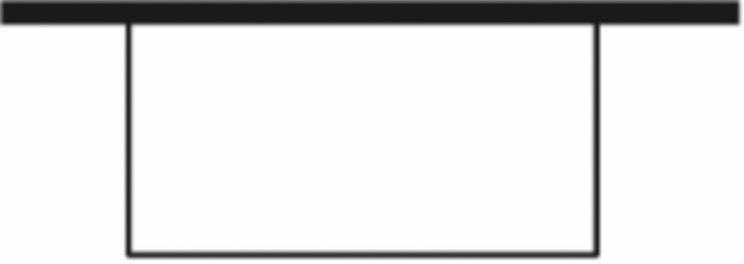
\includegraphics[width=0.28\textwidth]{figures/gao92_q8_fence.png}
\end{center}

\ifanswer
\solbegin
\step{设矩形的长为 $x$ 米，宽为 $y$，则 $xy=18$，}
\step{需要用栅栏长为 $x+2y\geqslant2\sqrt{2xy}=12$，}
\step{当且仅当 $x=2y$，即 $y=3$，$x=6$ 时取等号，故至少需要 $12$ 米栅栏.}
\solend
\fi

\item 已知 $a$ 为正整数，若关于 $x$ 的不等式 $\lvert x-2025\rvert\leqslant a$ 的解集中有且仅有 $7$ 个整数，则 $a$ 的值为\blankline[4.4em].

\ifanswer
\solbegin
\step{不等式 $\lvert x-2025\rvert\leqslant a$，则 $-a\leqslant x-2025\leqslant a$，即 $2025-a\leqslant x\leqslant2025+a$，}
\step{所以不等式 $\lvert x-2025\rvert\leqslant a$ 的解集为 $\{x\mid2025-a\leqslant x\leqslant2025+a\}$，}
\step{若不等式解集中有且仅有 $7$ 个整数，且 $a$ 为正整数，}
\step{由解集的对称性得这 $7$ 个整数以 $2025$ 为中心，向左右两边各延伸 $3$ 个整数，}
\step{即这 $7$ 个整数为 $2022,2023,2024,2025,2026,2027,2028$，所以 $a=3$.}
\solend
\fi

\item 已知关于 $x$ 的一元二次方程 $x^2-x+a=0$ 有两个不相等的正根 $m$、$n$，则 $\dfrac1m+\dfrac9n$ 的最小值为\blankline[4.4em].

\ifanswer
\solbegin
\step{因为一元二次方程 $x^2-x+a=0$ 有两个不相等的正根 $m$、$n$，}
\step{所以判别式 $\Delta=(-1)^2-4a>0\Rightarrow a<\dfrac14$，$m+n=1$，$mn=a>0$，}
\step{因此 $0<a<\dfrac14$ 且 $m+n=1(m,n>0)$.}
\step{$\dfrac1m+\dfrac9n=\left(\dfrac1m+\dfrac9n\right)(m+n)=1+\dfrac nm+\dfrac{9m}{n}+9=10+\dfrac nm+\dfrac{9m}{n}\geqslant10+2\sqrt9=16$，}
\step{等号成立条件为 $\dfrac nm=\dfrac{9m}{n}\Rightarrow n^2=9m^2\Rightarrow n=3m$，}
\step{$m$、$n>0$，结合 $m+n=1$，代入 $n=3m$ 得 $m+3m=1\Rightarrow m=\dfrac14$，$n=\dfrac34$，}
\step{此时 $mn=\dfrac14\cdot\dfrac34=\dfrac3{16}$，满足 $0<a<\dfrac14$，等号可取，因此 $\dfrac1m+\dfrac9n$ 的最小值为 $16$.}
\solend
\fi

\item 对任意 $A$、$B\subseteq R$，记 $A\oplus B=\{x\mid x\in A\cup B,x\notin A\cap B\}$，并称 $A\oplus B$ 为集合 $A$，$B$ 的对称差. 例如：若 $A=\{1,2,3\},B=\{2,3,4\}$，则 $A\oplus B=\{1,4\}$. 下列命题中，为真命题的有\blankline[4.4em].

①若 $A$、$B\subseteq R$ 且 $A\oplus B\subseteq A$，则 $A\subseteq B$

②若 $A$、$B\subseteq R$ 且 $A\oplus B=\varnothing$，则 $A=B$

③若 $A$、$B\subseteq R$ 且 $A\oplus B=B$，则 $A=\varnothing$

④对任意 $A$、$B\subseteq R$，都有 $A\oplus B=\complement_{R}A\oplus\complement_{R}B$

\ifanswer
\solbegin
\step{对于①，因为 $A\oplus B\subseteq A$，所以 $\{x\mid x\in A\cup B,x\notin A\cap B\}\subseteq A$，故 $B\subseteq A$，}
\step{故①错误；}
\step{对于②，$A$、$B\subseteq R$ 且 $A\oplus B=\varnothing$，则 $\varnothing=\{x\mid x\in A\cup B,x\notin A\cap B\}$，}
\step{即 $A\cup B=A\cap B$，所以 $A=B$，故②正确；}
\step{对于③，$A$、$B\subseteq R$ 且 $A\oplus B=B$，则 $B=\{x\mid x\in A\cup B,x\notin A\cap B\}$，}
\step{故 $A\subseteq B$，且 $B$ 中元素不在 $A\cap B$ 中，故 $A=\varnothing$，故③正确；}
\step{对于④，$\complement_{R}A\oplus\complement_{R}B=\{x\mid x\in\complement_{R}A\cup\complement_{R}B,x\notin\complement_{R}A\cap\complement_{R}B\}$，}
\step{其中 $\complement_{R}A\cup\complement_{R}B=\complement_{R}(A\cap B)$，$\complement_{R}A\cap\complement_{R}B=\complement_{R}(A\cup B)$，}
\step{故 $\complement_{R}A\oplus\complement_{R}B=\{x\mid x\in\complement_{R}(A\cap B)$，}
\step{$x\notin\complement_{R}(A\cup B)\}=\{x\mid x\in A\cup B,x\notin A\cap B\}$，}
\step{而 $A\oplus B=\{x\mid x\in A\cup B,x\notin A\cap B\}$，故 $A\oplus B=\complement_{R}A\oplus\complement_{R}B$，故④正确.}
\step{故正确的是②③④.}
\solend
\fi

\item 若不等式 $x^2-2ax+a^2-1\geqslant0$ 对任意 $x\in[0,2]$ 恒成立，则实数 $a$ 的取值范围是\blankline[4.4em].

\ifanswer
\solbegin
\step{由题意不等式 $x^2-2ax+a^2-1\geqslant0$ 对任意 $x\in[0,2]$ 恒成立，}
\step{解得 $x\leqslant a-1$ 或 $x\geqslant a+1$，要使此不等式对任意 $x\in[0,2]$ 恒成立，}
\step{则区间 $[0,2]$ 必须完全包含在解集 $(-\infty,a-1]\cup[a+1,+\infty)$ 中，}
\step{等价于 $[0,2]$ 与开区间 $(a-1,a+1)$ 的交集为空集，}
\step{区间 $[0,2]$ 在 $a-1$ 左侧，即 $2\leqslant a-1$，解得 $a\geqslant3$，}
\step{区间 $[0,2]$ 在 $a+1$ 右侧，即 $a+1\leqslant0$，解得 $a\leqslant-1$，}
\step{当 $a\in(-1,3)$，则 $(a-1,a+1)$ 与 $[0,2]$ 必有交集，不满足条件，}
\step{综上，实数 $a$ 的取值范围是 $(-\infty,-1]\cup[3,+\infty)$.}
\solend
\fi

\end{enumerate}

\bigsec{二、选择题}

\begin{enumerate}
\setcounter{enumi}{12}

\item 若 $a<b<0$，则下列不等式成立的是\mbox{（\quad）}% 原卷括号内已印“D”，试卷版按惯例留空

\keepwithprev
A. $a^2<b^2$\qquad B. $\dfrac1a<\dfrac1b$\qquad C. $ab<b^2$\qquad D. $ab<a^2$

\ifanswer
\ans{$D$}
\fi

\item 已知全集 $U=\{1,2,3,4,5\}$，集合 $A,B$ 是 $U$ 子集，满足 $\overline{A\cup B}=\{4,5\}$，$B=\{2,3\}$，则 $A\cap\overline B=\mbox{（\quad）}$

\keepwithprev
A. $\{1\}$\qquad B. $\{1,2\}$\qquad C. $\{1,4,5\}$\qquad D. $\varnothing$

\ifanswer
\solbegin
\step{因为全集 $U=\{1,2,3,4,5\}$，集合 $A$、$B$ 是 $U$ 子集，$\overline{A\cup B}=\{4,5\}$，$B=\{2,3\}$，}
\step{所以 $A\cup B=\{1,2,3\}$，故 $1\in A$，$1\notin B$，$4\notin A$，$5\notin A$，$4\notin B$，$5\notin B$，}
\step{故 $A\cap\overline B=\{1\}$. 故选 $A$.}
\solend
\fi

\item 设 $a>0$，若关于 $x$ 的不等式 $x^2-(2a-1)x-2a<0$ 的解集中恰有 $3$ 个整数，则实数 $a$ 的取值范围是\mbox{（\quad）}

\keepwithprev
A. $\left[1,\dfrac32\right]$\qquad B. $\left(1,\dfrac32\right]$\qquad C. $\left[\dfrac12,1\right]$\qquad D. $\left(\dfrac12,1\right]$

\ifanswer
\solbegin
\step{已知关于 $x$ 的不等式 $x^2-(2a-1)x-2a<0$，则 $(x+1)(x-2a)<0$，}
\step{则 $-1<x<2a$，又解集中恰有 $3$ 个整数，则 $2<2a\leqslant3$，则 $1<a\leqslant\dfrac32$，}
\step{则 $a$ 的取值范围为 $\left(1,\dfrac32\right]$. 故选 $B$.}
\solend
\fi

\item 已知集合 $U=\{1,2,3,\cdots,2027\}$，$M\subseteq U$，若对于 $M$ 中的任意两个不同的元素 $x$、$y$，都有 $\lvert x-y\rvert>2$，则 $M$ 中元素个数的最大值为\mbox{（\quad）}

\keepwithprev
A. $675$\qquad B. $676$\qquad C. $2025$\qquad D. $2026$

\ifanswer
\solbegin
\step{对于 $M$ 中的任意两个不同的元素 $x$、$y$，都有 $\lvert x-y\rvert>2$，}
\step{不妨设 $x>y$，都有 $x-y\geqslant3$，}
\step{要想 $M$ 所含元素个数最大，则要 $x-y$ 尽可能小，故需使得 $x-y$ 的最小值为 $3$，}
\step{将 $1\sim2027$ 这 $2027$ 个元素按如下分组：}
\step{$\{1,2,3\},\{4,5,6\},\cdots,\{2023,2024,2025\},\{2026,2027\}$，}
\step{故应在前 $675$ 组中按周期 $3$ 每组取一个元素，且第一组中不能取 $3$，}
\step{第一组中取 $1$ 时，得 $M=\{1,4,7,\cdots,2023,2026\}$}
\step{或 $M=\{1,4,7,\cdots,2023,2027\}$ 这样的集合，}
\step{第一组取 $2$ 时，得 $M=\{2,5,8,\cdots,2024,2027\}$，}
\step{其中任意两元素差值 $x-y(x>y)$ 都大于 $2$，满足题意，}
\step{故 $M$ 所含元素个数的最大值为 $\dfrac{2025}{3}+1=676$. 故选 $B$.}
\solend
\fi

\end{enumerate}

\bigsec{三、解答题}

\begin{enumerate}
\setcounter{enumi}{16}

\item 已知集合 $M=\{x\mid a-1\leqslant x\leqslant2a+3\}$，$P=\{x\mid-2<x\leqslant4\}$，全集 $U=R$.

（1）当 $a=2$ 时，求 $M\cap P$；

（2）若 $x\in P$ 是 $x\in M$ 的必要不充分条件，求实数 $a$ 的取值范围.

\ansspace*[9]

\ifanswer
\solbegin
\stepm{（1）}{当 $a=2$ 时，集合 $M=\{x\mid1\leqslant x\leqslant7\}$，所以 $M\cap P=\{x\mid1\leqslant x\leqslant4\}$；}
\stepm{（2）}{因为 $x\in P$ 是 $x\in M$ 的必要不充分条件，所以 $M\subsetneqq P$，}
\step{当 $M=\varnothing$ 时，$a-1>2a+3$，解得 $a<-4$，}
\step{当 $M\neq\varnothing$ 时，则 $\begin{cases}a-1\leqslant2a+3\\ a-1>-2\\ 2a+3\leqslant4\end{cases}$，解得 $-1<a\leqslant\dfrac12$，}
\step{综上所述，实数 $a$ 的取值范围为 $(-\infty,-4)\cup\left(-1,\dfrac12\right]$.}
\solend
\fi

\item 命题甲：关于 $x$ 的方程 $(a-1)x^2+(2a-4)x+a=0$ 有两个不相等的实数根；

命题乙：关于 $x$ 的不等式 $ax^2-2ax+a+1>0$ 的解集为 $R$.

（1）若命题甲为真命题，求实数 $a$ 的取值范围；

（2）若命题甲、乙中至多有一个为真命题，求实数 $a$ 的取值范围.

\ansspace*[12]

\ifanswer
\solbegin
\stepm{（1）}{命题甲：关于 $x$ 的方程 $(a-1)x^2+(2a-4)x+a=0$ 有两个不相等的实数根，}
\step{则 $\begin{cases}a-1\neq0\\ \Delta=(2a-4)^2-4a(a-1)>0\end{cases}$，解得 $a<\dfrac43$ 且 $a\neq1$，}
\step{故 $a$ 的范围为 $\left\{a\left|a<\dfrac43\ \text{且}\ a\neq1\right.\right\}$；}
\stepm{（2）}{当 $a=0$ 时 $y=1>0$，符合题意；}
\step{当 $a\neq0$，由 $\begin{cases}a>0\\ \Delta=4a^2-4a(a+1)<0\end{cases}$，解得 $a>0$，}
\step{则 $a$ 的取值范围为 $a\geqslant0$，}
\step{故 $p$、$q$ 都为真时，$a$ 的范围为 $0\leqslant a<\dfrac43$ 且 $a\neq1$，}
\step{则命题甲、乙中至多有一个为真命题时，}
\step{$a$ 的取值范围为 $\left\{a\left|a<0\ \text{或}\ a=1\ \text{或}\ a\geqslant\dfrac43\right.\right\}$.}
\solend
\fi

\item 如图，$OA$、$OB$ 是两条长度足够长的互相垂直的笔直小路，矩形 $OCPD$ 的顶点 $C$，$D$ 分别在 $OA$、$OB$ 上，且该矩形区域内种满了荷花. 为了让观赏者有更好的观赏体验，现计划经过点 $P$ 修一条小路 $EF$，其中点 $E$ 在小路 $OA$ 上，点 $F$ 在小路 $OB$ 上，并在 $\triangle OEF$ 区域内种满荷花. 已知 $OD=25$ m，$OC=40$ m，且小路 $EF$ 要完全位于一个以 $O$ 为顶点的，边长为 $100$ m 的正方形内部（包括边界）. 记 $\triangle OEF$ 的面积为 $S$ m$^2$.

\begin{center}
\begin{tikzpicture}[x=0.46cm,y=0.42cm,line width=0.7pt]
\draw (0,0) -- (0,10.2) node[above,inner sep=3pt] {$A$};
\draw (0,0) -- (11.8,0) node[right,inner sep=3pt] {$B$};
\draw (0,4.83) -- (2.42,4.83) -- (2.42,0);
\draw (0,6.92) -- (8.01,0);
\node[below left,inner sep=2pt] at (0,0) {$O$};
\node[below,inner sep=2pt] at (2.42,0) {$D$};
\node[left,inner sep=3pt] at (0,4.83) {$C$};
\node[above right,inner sep=1pt] at (2.42,4.83) {$P$};
\node[left,inner sep=3pt] at (0,6.92) {$E$};
\node[below,inner sep=2pt] at (8.01,0) {$F$};
\end{tikzpicture}
\end{center}

（1）设 $EC=x\cdot m$，试用 $x$ 表示 $OF$，并求 $x$ 的取值范围.

（2）当 $EC$ 的长度为多少时，$S$ 取得最小值？最小值是多少？

\ansspace*[11]

\ifanswer
\solbegin
\stepm{（1）}{由题意得 $x\leqslant60$，}
\step{$\triangle PCE\backsim\triangle FDP$，所以 $\dfrac{EC}{CP}=\dfrac{PD}{DF}$，即 $\dfrac{x}{25}=\dfrac{40}{DF}$，得 $DF=\dfrac{1000}{x}$ m，}
\step{所以 $OF=OD+DF=\left(25+\dfrac{1000}{x}\right)$ m，}
\step{所以 $25+\dfrac{1000}{x}\leqslant100$，解得 $x\geqslant\dfrac{40}{3}$；}
\step{综上，$\dfrac{40}{3}\leqslant x\leqslant60$；}
\stepm{（2）}{由 $OE=OC+CE=(40+x)$ m，}
\step{所以 $S=\dfrac12\cdot OF\cdot OE=\dfrac12\left(25+\dfrac{1000}{x}\right)(40+x)$}
\step{$=\dfrac12\left(1000+25x+\dfrac{40000}{x}+1000\right)$ m$^2$，}
\step{由基本不等式得 $S\geqslant\dfrac12\left(2000+2\sqrt{25x\cdot\dfrac{40000}{x}}\right)=2000$ m$^2$，}
\step{当且仅当 $25x=\dfrac{40000}{x}$，即 $x=40$ 时取等号，}
\step{故 $EC=40$ m 时，$S$ 取得最小值，为 $2000$ m$^2$.}
\solend
\fi

\item 已知函数 $f(x)=x^2-(a-2)x+a-3$.

（1）若 $f(x)=0$ 的两根为 $\alpha,\beta$，$\alpha^2+\beta^2=2$，求 $a$ 的值；

（2）解关于 $x$ 的不等式 $f(x)\geqslant0$；

（3）是否存在整数 $m,n$，使得关于 $x$ 的不等式 $m\leqslant f(x)\leqslant n$ 的解集恰好为 $[m,n]$？若存在，求出 $m,n$ 的值. 若不存在，请说明理由.

\ansspace*[16]

\ifanswer
\solbegin
\stepm{（1）}{由韦达定理，$\alpha+\beta=a-2,\alpha\beta=a-3$，}
\step{因此 $\alpha^2+\beta^2=(a-2)^2-2(a-3)=2\Leftrightarrow(a-2)(a-4)=0$，}
\step{$a=2$ 时两根为 $1,-1$；$a=4$ 时两根均为 $1$，均满足条件，}
\step{所以 $a=2$ 或 $a=4$.}
\stepm{（2）}{因为 $f(x)=(x-1)[x-(a-3)]$，所以分三种情况：}
\step{当 $a<4$ 时，$a-3<1$，解集为 $(-\infty,a-3]\cup[1,+\infty)$.}
\step{当 $a=4$ 时，$f(x)=(x-1)^2\geqslant0$ 恒成立，解集为 $R$.}
\step{当 $a>4$ 时，$a-3>1$，解集为 $(-\infty,1]\cup[a-3,+\infty)$.}
\stepm{（3）}{区间 $[m,n]$ 要求 $m<n$. 记 $f(x)$ 的最小值为 $k$.}
\step{$[m,n]$ 非空，不等式 $f(x)\leqslant n$ 有解，其解集为闭区间 $[x_1,x_2]$，}
\step{其中 $x_1\leqslant x_2$ 是方程 $f(x)=n$ 的两根.}
\step{若 $k<m$，则 $f(x)<m$ 的解集是 $[x_1,x_2]$ 内部的一个开区间，}
\step{从 $[x_1,x_2]$ 中去掉它后剩下两段，原不等式的解集不是一个区间，矛盾，}
\step{所以 $k\geqslant m$，原不等式的解集就是 $[x_1,x_2]$，于是 $m=x_1,n=x_2$，}
\step{即 $f(m)=f(n)=n$，于是 $f(m)-f(n)=(m-n)(m+n-a+2)=0$.}
\step{因为 $m\neq n$，所以 $a=m+n+2$.}
\step{代入 $f(m)=n$，得 $(m-1)(1-n)=n\Leftrightarrow m(n-1)=-1$，$m,n$ 均为整数，}
\step{因此 $(m,n)=(-1,2)$ 或 $(m,n)=(1,0)$.}
\step{结合 $m<n$，只可能有 $m=-1,n=2$，此时 $a=3$.}
\step{检验：此时 $f(x)=x^2-x$，且 $x^2-x=\left(x-\dfrac12\right)^2-\dfrac14\geqslant-\dfrac14>-1$，}
\step{因此 $-1\leqslant f(x)\leqslant2\Leftrightarrow x^2-x\leqslant2\Leftrightarrow(x+1)(x-2)\leqslant0\Leftrightarrow x\in[-1,2]$，}
\step{所以存在符合条件的整数 $m=-1,n=2$.}
\solend
\fi

\item 给定数集 $M$，若对于任意 $a$、$b\in M$，有 $a+b\in M,a-b\in M$，则称集合 $M$ 为闭集合.

（1）判断集合 $A_1=\{-4,-2,0,2,4\}$，集合 $B=\{x\mid x=3k,k\in\Z\}$ 是否为闭集合；

（2）若集合 $C$、$D$ 为闭集合，则 $C\cup D$ 是否一定为闭集合？请说明理由；

（3）已知集合 $C$、$D$ 为闭集合，且 $C\subsetneq R,D\subsetneq R$，证明：$(C\cup D)\subsetneq R$.% 原卷印作 (C∪D)⊂R，按解析证明的是 C∪D≠R，排真子集

\ansspace*[14]

\ifanswer
\solbegin
\stepm{（1）}{因为 $4\in A_1$，$2\in A_1$，$4+2=6\notin A_1$，所以 $A_1$ 不是闭集合；}
\step{任取 $x,y\in B$，设 $x=3m,y=3n,m,n\in\Z$，}
\step{则 $x+y=3m+3n=3(m+n)$ 且 $m+n\in\Z$，}
\step{所以 $x+y\in B$，同理，$x-y\in B$，故 $B$ 为闭集合.}
\stepm{（2）}{结论：不一定.}
\step{不妨令 $C=\{x\mid x=2k,k\in\Z\},D=\{x\mid x=3k,k\in\Z\}$，}
\step{则由（1）得 $C$、$D$ 为闭集合，易得 $2,3\in C\cup D,2+3=5\notin C\cup D$，}
\step{因此，$C\cup D$ 不一定是闭集合.}
\stepm{（3）}{不妨假设 $C\cup D=R$，则由 $C\subsetneq R$，得存在 $a\in R$ 且 $a\notin C$，故 $a\in D$.}
\step{同理，存在 $b\in R$ 且 $b\notin D$，故 $b\in C$.}
\step{因为 $a+b\in R=C\cup D$，所以 $a+b\in C$ 或 $a+b\in D$.}
\step{若 $a+b\in C$，则由 $C$ 为闭集合且 $b\in C$，得 $a=(a+b)-b\in C$，}
\step{与 $a\notin C$ 矛盾.}
\step{若 $a+b\in D$，则由 $D$ 为闭集合且 $a\in D$，得 $b=(a+b)-a\in D$，}
\step{与 $b\notin D$ 矛盾.}
\step{综上，$C\cup D=R$ 不成立，故 $(C\cup D)\subsetneq R$.}
\solend
\fi

\end{enumerate}

\end{document}
"
%
% 原始材料：微信公众号“魔都数学加油站”文章，连载“27学年高一92”；
% 原文标题“27学年高一92——2026-2027年上海市闵行实验高一上10月月考”；
% 原文链接：https://mp.weixin.qq.com/s/8HUyr3G7GpcHyczwu_XYCQ。
% 正文为 10 张 PNG 页（`原图/高一92_闵行实验_10月月考/01..10.png`），均 4762×6735，按页序读取。
%
% 篇幅与题号：原卷自第 3 题起编号（第 1、2 题不在原文内）。填空题 3—12（10 题）、
% 选择题 13—16（4 题）、解答题 17—21（5 题），共 19 题。
%
% 讲评版：第 6 题只印【答案】（“$[-1,3]$”），本稿只给 \ans{}；第 13 题无【解析】、
% 答案“D”直接印在题干括号内，本稿试卷版按惯例留空、答案版提 \ans{$D$}；其余 17 题印
% 【解析】，其中选择题答案在解析末句“故选 $A$／$B$／$B$”。
% 第 8 题题干右侧有一幅“围墙 + 三面栅栏”示意图（裁自第 2 页原图）；第 19 题题干带
% 与 高一88 第 19 题同型的示意图（$OA$／$OB$ 两条小路、矩形 $OCPD$、折线 $EF$），用 TikZ 重绘。
%
% 副标题：原卷未印副标题。本稿按内容标作“集合与常用逻辑用语、不等式”。
%
% 原卷笔误/存疑（均照录未改，正文对应处另有 % 注）：
%   ① 第 21 题 (3) 题干与解析末句把结论印作“$(C\cup D)\subset R$”，而解析证明的是
%      “$C\cup D=\R$ 不成立”，按文意应为“$(C\cup D)\subsetneq\R$”；本稿按真子集排
%      $\subsetneq$，原卷记号照录于文件头；
%   ② 第 7 题解析只列 $B=\varnothing$（$a=0$）、$B=\{1\}$（$a=1$）、$B=\{-3\}$（$a=-\frac13$）
%      三种情形，与结论 $\left\{0,1,-\frac13\right\}$ 相符，无笔误。
%
% 与原卷的排版差异：
%   ① 原卷每题下直接印【答案】/【解析】，本稿按全稿惯例将答案与解析置于答案版；
%   ② 原卷未印副标题，本稿补出；填空横线统一排 \blankline[4.4em]；
%   ③ 原卷数集记号排斜体 $R$、$Z$，本稿按全稿惯例改用 $\R$、$\Z$；
%   ④ 第 17—21 题的子问用行内“（1）（2）（3）”段，解析中的子问标号用 \stepm；
%   ⑤ 解答题按惯例加 \ansspace；选择题括号排 \mbox{（\quad）}；
%   ⑥ 第 8 题的示意图原卷排在题干右侧、文字绕排，本稿改排为题干后的居中图
%      （自原图裁切、去粉色水印后转灰度）；第 19 题的图按原图比例 TikZ 重绘。
%
% 行数核对：逐题数 \step/\stepm 条数，合计 128 条（Q3：2；Q4：3；Q5：2；Q6：0；Q7：6；
% Q8：3；Q9：5；Q10：7；Q11：12；Q12：8；Q13：0；Q14：3；Q15：3；Q16：11；Q17：5；
% Q18：9；Q19：11；Q20：22；Q21：16）。第 6 题只印答案、第 13 题无解析，均不计入 \step 账。
% 原卷解析的换行按语意合并，未逐行强拆。
%
\documentclass[a4paper,11pt]{article}
\usepackage{common}

\begin{document}

\examtitlest[7]{2026--2027 年闵行实验高一上 10 月月考}{集合与常用逻辑用语、不等式}

\bigsec{一、填空题}

\begin{enumerate}
\setcounter{enumi}{2}

\item 已知 $3<a<8$，$4<b<9$，则 $\dfrac ab$ 的取值范围是\blankline[4.4em].

\ifanswer
\solbegin
\step{因为 $4<b<9$，所以 $\dfrac19<\dfrac1b<\dfrac14$，又 $3<a<8$，所以 $\dfrac13<\dfrac ab<2$，}
\step{故 $\dfrac ab$ 的取值范围是 $\left(\dfrac13,2\right)$.}
\solend
\fi

\item 已知 $p:x>3$，$q:x>5$，则 $p$ 是 $q$ 的\blankline[4.4em]（选“充分不必要条件”“必要不充分条件”“充要条件”“既不充分也不必要条件”之一填空）.

\ifanswer
\solbegin
\step{当 $x>3$ 时，不能推出 $x>5$，充分性不成立；}
\step{当 $x>5$ 时，可以得到 $x>3$，必要性成立；}
\step{故 $p$ 是 $q$ 的必要不充分条件.}
\solend
\fi

\item 不等式 $\dfrac{x-1}{2x+1}\leqslant1$ 的解集为\blankline[4.4em].

\ifanswer
\solbegin
\step{因为 $\dfrac{x-1}{2x+1}\leqslant1$，所以 $\dfrac{x-1}{2x+1}-\dfrac{2x+1}{2x+1}\leqslant0$，所以 $\dfrac{x+2}{2x+1}\geqslant0$，}
\step{所以 $x>-\dfrac12$ 或 $x\leqslant-2$，即不等式的解集是 $(-\infty,-2]\cup\left(-\dfrac12,+\infty\right)$.}
\solend
\fi

\item 设 $x\in R$，则方程 $\lvert x+1\rvert+\lvert x-3\rvert=4$ 的解集为\blankline[4.4em].

\ifanswer
\ans{$[-1,3]$}
\fi

\item 若 $A=\{x\mid x^2+2x=3\}$，$B=\{x\mid ax=1\}$，且 $B\subseteq A$，则实数 $a$ 的值组成的集合为\blankline[4.4em].

\ifanswer
\solbegin
\step{由 $x^2+2x=3$ 得 $x^2+2x-3=0$，解得 $x=1$ 或 $x=-3$，所以 $A=\{1,-3\}$，}
\step{又因为 $B=\{x\mid ax=1\}$，且 $B\subseteq A$，}
\step{当 $B=\varnothing$，即 $a=0$ 时，显然符合题意；}
\step{当 $B=\{1\}$，即 $a=1$ 时，也符合题意；}
\step{当 $B=\{-3\}$，即 $a=-\dfrac13$ 时，也符合题意；}
\step{综上所述，实数 $a$ 的值组成的集合为 $\left\{0,1,-\dfrac13\right\}$.}
\solend
\fi

\item 某校欲在围墙边用栅栏围成一个 $18$ 平方米的矩形区域，作为天鹅的地面栖息地，矩形区域的一条边为围墙（如图），则至少需要\blankline[4.4em]米栅栏.

\begin{center}
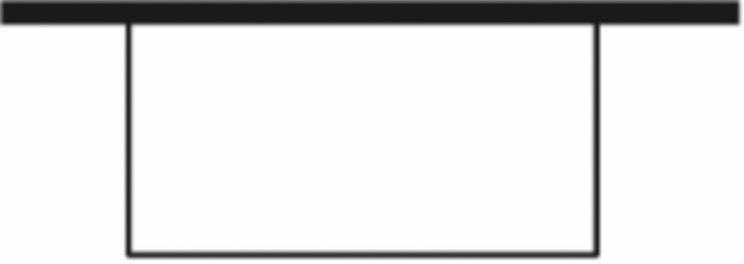
\includegraphics[width=0.28\textwidth]{figures/gao92_q8_fence.png}
\end{center}

\ifanswer
\solbegin
\step{设矩形的长为 $x$ 米，宽为 $y$，则 $xy=18$，}
\step{需要用栅栏长为 $x+2y\geqslant2\sqrt{2xy}=12$，}
\step{当且仅当 $x=2y$，即 $y=3$，$x=6$ 时取等号，故至少需要 $12$ 米栅栏.}
\solend
\fi

\item 已知 $a$ 为正整数，若关于 $x$ 的不等式 $\lvert x-2025\rvert\leqslant a$ 的解集中有且仅有 $7$ 个整数，则 $a$ 的值为\blankline[4.4em].

\ifanswer
\solbegin
\step{不等式 $\lvert x-2025\rvert\leqslant a$，则 $-a\leqslant x-2025\leqslant a$，即 $2025-a\leqslant x\leqslant2025+a$，}
\step{所以不等式 $\lvert x-2025\rvert\leqslant a$ 的解集为 $\{x\mid2025-a\leqslant x\leqslant2025+a\}$，}
\step{若不等式解集中有且仅有 $7$ 个整数，且 $a$ 为正整数，}
\step{由解集的对称性得这 $7$ 个整数以 $2025$ 为中心，向左右两边各延伸 $3$ 个整数，}
\step{即这 $7$ 个整数为 $2022,2023,2024,2025,2026,2027,2028$，所以 $a=3$.}
\solend
\fi

\item 已知关于 $x$ 的一元二次方程 $x^2-x+a=0$ 有两个不相等的正根 $m$、$n$，则 $\dfrac1m+\dfrac9n$ 的最小值为\blankline[4.4em].

\ifanswer
\solbegin
\step{因为一元二次方程 $x^2-x+a=0$ 有两个不相等的正根 $m$、$n$，}
\step{所以判别式 $\Delta=(-1)^2-4a>0\Rightarrow a<\dfrac14$，$m+n=1$，$mn=a>0$，}
\step{因此 $0<a<\dfrac14$ 且 $m+n=1(m,n>0)$.}
\step{$\dfrac1m+\dfrac9n=\left(\dfrac1m+\dfrac9n\right)(m+n)=1+\dfrac nm+\dfrac{9m}{n}+9=10+\dfrac nm+\dfrac{9m}{n}\geqslant10+2\sqrt9=16$，}
\step{等号成立条件为 $\dfrac nm=\dfrac{9m}{n}\Rightarrow n^2=9m^2\Rightarrow n=3m$，}
\step{$m$、$n>0$，结合 $m+n=1$，代入 $n=3m$ 得 $m+3m=1\Rightarrow m=\dfrac14$，$n=\dfrac34$，}
\step{此时 $mn=\dfrac14\cdot\dfrac34=\dfrac3{16}$，满足 $0<a<\dfrac14$，等号可取，因此 $\dfrac1m+\dfrac9n$ 的最小值为 $16$.}
\solend
\fi

\item 对任意 $A$、$B\subseteq R$，记 $A\oplus B=\{x\mid x\in A\cup B,x\notin A\cap B\}$，并称 $A\oplus B$ 为集合 $A$，$B$ 的对称差. 例如：若 $A=\{1,2,3\},B=\{2,3,4\}$，则 $A\oplus B=\{1,4\}$. 下列命题中，为真命题的有\blankline[4.4em].

①若 $A$、$B\subseteq R$ 且 $A\oplus B\subseteq A$，则 $A\subseteq B$

②若 $A$、$B\subseteq R$ 且 $A\oplus B=\varnothing$，则 $A=B$

③若 $A$、$B\subseteq R$ 且 $A\oplus B=B$，则 $A=\varnothing$

④对任意 $A$、$B\subseteq R$，都有 $A\oplus B=\complement_{R}A\oplus\complement_{R}B$

\ifanswer
\solbegin
\step{对于①，因为 $A\oplus B\subseteq A$，所以 $\{x\mid x\in A\cup B,x\notin A\cap B\}\subseteq A$，故 $B\subseteq A$，}
\step{故①错误；}
\step{对于②，$A$、$B\subseteq R$ 且 $A\oplus B=\varnothing$，则 $\varnothing=\{x\mid x\in A\cup B,x\notin A\cap B\}$，}
\step{即 $A\cup B=A\cap B$，所以 $A=B$，故②正确；}
\step{对于③，$A$、$B\subseteq R$ 且 $A\oplus B=B$，则 $B=\{x\mid x\in A\cup B,x\notin A\cap B\}$，}
\step{故 $A\subseteq B$，且 $B$ 中元素不在 $A\cap B$ 中，故 $A=\varnothing$，故③正确；}
\step{对于④，$\complement_{R}A\oplus\complement_{R}B=\{x\mid x\in\complement_{R}A\cup\complement_{R}B,x\notin\complement_{R}A\cap\complement_{R}B\}$，}
\step{其中 $\complement_{R}A\cup\complement_{R}B=\complement_{R}(A\cap B)$，$\complement_{R}A\cap\complement_{R}B=\complement_{R}(A\cup B)$，}
\step{故 $\complement_{R}A\oplus\complement_{R}B=\{x\mid x\in\complement_{R}(A\cap B)$，}
\step{$x\notin\complement_{R}(A\cup B)\}=\{x\mid x\in A\cup B,x\notin A\cap B\}$，}
\step{而 $A\oplus B=\{x\mid x\in A\cup B,x\notin A\cap B\}$，故 $A\oplus B=\complement_{R}A\oplus\complement_{R}B$，故④正确.}
\step{故正确的是②③④.}
\solend
\fi

\item 若不等式 $x^2-2ax+a^2-1\geqslant0$ 对任意 $x\in[0,2]$ 恒成立，则实数 $a$ 的取值范围是\blankline[4.4em].

\ifanswer
\solbegin
\step{由题意不等式 $x^2-2ax+a^2-1\geqslant0$ 对任意 $x\in[0,2]$ 恒成立，}
\step{解得 $x\leqslant a-1$ 或 $x\geqslant a+1$，要使此不等式对任意 $x\in[0,2]$ 恒成立，}
\step{则区间 $[0,2]$ 必须完全包含在解集 $(-\infty,a-1]\cup[a+1,+\infty)$ 中，}
\step{等价于 $[0,2]$ 与开区间 $(a-1,a+1)$ 的交集为空集，}
\step{区间 $[0,2]$ 在 $a-1$ 左侧，即 $2\leqslant a-1$，解得 $a\geqslant3$，}
\step{区间 $[0,2]$ 在 $a+1$ 右侧，即 $a+1\leqslant0$，解得 $a\leqslant-1$，}
\step{当 $a\in(-1,3)$，则 $(a-1,a+1)$ 与 $[0,2]$ 必有交集，不满足条件，}
\step{综上，实数 $a$ 的取值范围是 $(-\infty,-1]\cup[3,+\infty)$.}
\solend
\fi

\end{enumerate}

\bigsec{二、选择题}

\begin{enumerate}
\setcounter{enumi}{12}

\item 若 $a<b<0$，则下列不等式成立的是\mbox{（\quad）}% 原卷括号内已印“D”，试卷版按惯例留空

\keepwithprev
A. $a^2<b^2$\qquad B. $\dfrac1a<\dfrac1b$\qquad C. $ab<b^2$\qquad D. $ab<a^2$

\ifanswer
\ans{$D$}
\fi

\item 已知全集 $U=\{1,2,3,4,5\}$，集合 $A,B$ 是 $U$ 子集，满足 $\overline{A\cup B}=\{4,5\}$，$B=\{2,3\}$，则 $A\cap\overline B=\mbox{（\quad）}$

\keepwithprev
A. $\{1\}$\qquad B. $\{1,2\}$\qquad C. $\{1,4,5\}$\qquad D. $\varnothing$

\ifanswer
\solbegin
\step{因为全集 $U=\{1,2,3,4,5\}$，集合 $A$、$B$ 是 $U$ 子集，$\overline{A\cup B}=\{4,5\}$，$B=\{2,3\}$，}
\step{所以 $A\cup B=\{1,2,3\}$，故 $1\in A$，$1\notin B$，$4\notin A$，$5\notin A$，$4\notin B$，$5\notin B$，}
\step{故 $A\cap\overline B=\{1\}$. 故选 $A$.}
\solend
\fi

\item 设 $a>0$，若关于 $x$ 的不等式 $x^2-(2a-1)x-2a<0$ 的解集中恰有 $3$ 个整数，则实数 $a$ 的取值范围是\mbox{（\quad）}

\keepwithprev
A. $\left[1,\dfrac32\right]$\qquad B. $\left(1,\dfrac32\right]$\qquad C. $\left[\dfrac12,1\right]$\qquad D. $\left(\dfrac12,1\right]$

\ifanswer
\solbegin
\step{已知关于 $x$ 的不等式 $x^2-(2a-1)x-2a<0$，则 $(x+1)(x-2a)<0$，}
\step{则 $-1<x<2a$，又解集中恰有 $3$ 个整数，则 $2<2a\leqslant3$，则 $1<a\leqslant\dfrac32$，}
\step{则 $a$ 的取值范围为 $\left(1,\dfrac32\right]$. 故选 $B$.}
\solend
\fi

\item 已知集合 $U=\{1,2,3,\cdots,2027\}$，$M\subseteq U$，若对于 $M$ 中的任意两个不同的元素 $x$、$y$，都有 $\lvert x-y\rvert>2$，则 $M$ 中元素个数的最大值为\mbox{（\quad）}

\keepwithprev
A. $675$\qquad B. $676$\qquad C. $2025$\qquad D. $2026$

\ifanswer
\solbegin
\step{对于 $M$ 中的任意两个不同的元素 $x$、$y$，都有 $\lvert x-y\rvert>2$，}
\step{不妨设 $x>y$，都有 $x-y\geqslant3$，}
\step{要想 $M$ 所含元素个数最大，则要 $x-y$ 尽可能小，故需使得 $x-y$ 的最小值为 $3$，}
\step{将 $1\sim2027$ 这 $2027$ 个元素按如下分组：}
\step{$\{1,2,3\},\{4,5,6\},\cdots,\{2023,2024,2025\},\{2026,2027\}$，}
\step{故应在前 $675$ 组中按周期 $3$ 每组取一个元素，且第一组中不能取 $3$，}
\step{第一组中取 $1$ 时，得 $M=\{1,4,7,\cdots,2023,2026\}$}
\step{或 $M=\{1,4,7,\cdots,2023,2027\}$ 这样的集合，}
\step{第一组取 $2$ 时，得 $M=\{2,5,8,\cdots,2024,2027\}$，}
\step{其中任意两元素差值 $x-y(x>y)$ 都大于 $2$，满足题意，}
\step{故 $M$ 所含元素个数的最大值为 $\dfrac{2025}{3}+1=676$. 故选 $B$.}
\solend
\fi

\end{enumerate}

\bigsec{三、解答题}

\begin{enumerate}
\setcounter{enumi}{16}

\item 已知集合 $M=\{x\mid a-1\leqslant x\leqslant2a+3\}$，$P=\{x\mid-2<x\leqslant4\}$，全集 $U=R$.

（1）当 $a=2$ 时，求 $M\cap P$；

（2）若 $x\in P$ 是 $x\in M$ 的必要不充分条件，求实数 $a$ 的取值范围.

\ansspace*[9]

\ifanswer
\solbegin
\stepm{（1）}{当 $a=2$ 时，集合 $M=\{x\mid1\leqslant x\leqslant7\}$，所以 $M\cap P=\{x\mid1\leqslant x\leqslant4\}$；}
\stepm{（2）}{因为 $x\in P$ 是 $x\in M$ 的必要不充分条件，所以 $M\subsetneqq P$，}
\step{当 $M=\varnothing$ 时，$a-1>2a+3$，解得 $a<-4$，}
\step{当 $M\neq\varnothing$ 时，则 $\begin{cases}a-1\leqslant2a+3\\ a-1>-2\\ 2a+3\leqslant4\end{cases}$，解得 $-1<a\leqslant\dfrac12$，}
\step{综上所述，实数 $a$ 的取值范围为 $(-\infty,-4)\cup\left(-1,\dfrac12\right]$.}
\solend
\fi

\item 命题甲：关于 $x$ 的方程 $(a-1)x^2+(2a-4)x+a=0$ 有两个不相等的实数根；

命题乙：关于 $x$ 的不等式 $ax^2-2ax+a+1>0$ 的解集为 $R$.

（1）若命题甲为真命题，求实数 $a$ 的取值范围；

（2）若命题甲、乙中至多有一个为真命题，求实数 $a$ 的取值范围.

\ansspace*[12]

\ifanswer
\solbegin
\stepm{（1）}{命题甲：关于 $x$ 的方程 $(a-1)x^2+(2a-4)x+a=0$ 有两个不相等的实数根，}
\step{则 $\begin{cases}a-1\neq0\\ \Delta=(2a-4)^2-4a(a-1)>0\end{cases}$，解得 $a<\dfrac43$ 且 $a\neq1$，}
\step{故 $a$ 的范围为 $\left\{a\left|a<\dfrac43\ \text{且}\ a\neq1\right.\right\}$；}
\stepm{（2）}{当 $a=0$ 时 $y=1>0$，符合题意；}
\step{当 $a\neq0$，由 $\begin{cases}a>0\\ \Delta=4a^2-4a(a+1)<0\end{cases}$，解得 $a>0$，}
\step{则 $a$ 的取值范围为 $a\geqslant0$，}
\step{故 $p$、$q$ 都为真时，$a$ 的范围为 $0\leqslant a<\dfrac43$ 且 $a\neq1$，}
\step{则命题甲、乙中至多有一个为真命题时，}
\step{$a$ 的取值范围为 $\left\{a\left|a<0\ \text{或}\ a=1\ \text{或}\ a\geqslant\dfrac43\right.\right\}$.}
\solend
\fi

\item 如图，$OA$、$OB$ 是两条长度足够长的互相垂直的笔直小路，矩形 $OCPD$ 的顶点 $C$，$D$ 分别在 $OA$、$OB$ 上，且该矩形区域内种满了荷花. 为了让观赏者有更好的观赏体验，现计划经过点 $P$ 修一条小路 $EF$，其中点 $E$ 在小路 $OA$ 上，点 $F$ 在小路 $OB$ 上，并在 $\triangle OEF$ 区域内种满荷花. 已知 $OD=25$ m，$OC=40$ m，且小路 $EF$ 要完全位于一个以 $O$ 为顶点的，边长为 $100$ m 的正方形内部（包括边界）. 记 $\triangle OEF$ 的面积为 $S$ m$^2$.

\begin{center}
\begin{tikzpicture}[x=0.46cm,y=0.42cm,line width=0.7pt]
\draw (0,0) -- (0,10.2) node[above,inner sep=3pt] {$A$};
\draw (0,0) -- (11.8,0) node[right,inner sep=3pt] {$B$};
\draw (0,4.83) -- (2.42,4.83) -- (2.42,0);
\draw (0,6.92) -- (8.01,0);
\node[below left,inner sep=2pt] at (0,0) {$O$};
\node[below,inner sep=2pt] at (2.42,0) {$D$};
\node[left,inner sep=3pt] at (0,4.83) {$C$};
\node[above right,inner sep=1pt] at (2.42,4.83) {$P$};
\node[left,inner sep=3pt] at (0,6.92) {$E$};
\node[below,inner sep=2pt] at (8.01,0) {$F$};
\end{tikzpicture}
\end{center}

（1）设 $EC=x\cdot m$，试用 $x$ 表示 $OF$，并求 $x$ 的取值范围.

（2）当 $EC$ 的长度为多少时，$S$ 取得最小值？最小值是多少？

\ansspace*[11]

\ifanswer
\solbegin
\stepm{（1）}{由题意得 $x\leqslant60$，}
\step{$\triangle PCE\backsim\triangle FDP$，所以 $\dfrac{EC}{CP}=\dfrac{PD}{DF}$，即 $\dfrac{x}{25}=\dfrac{40}{DF}$，得 $DF=\dfrac{1000}{x}$ m，}
\step{所以 $OF=OD+DF=\left(25+\dfrac{1000}{x}\right)$ m，}
\step{所以 $25+\dfrac{1000}{x}\leqslant100$，解得 $x\geqslant\dfrac{40}{3}$；}
\step{综上，$\dfrac{40}{3}\leqslant x\leqslant60$；}
\stepm{（2）}{由 $OE=OC+CE=(40+x)$ m，}
\step{所以 $S=\dfrac12\cdot OF\cdot OE=\dfrac12\left(25+\dfrac{1000}{x}\right)(40+x)$}
\step{$=\dfrac12\left(1000+25x+\dfrac{40000}{x}+1000\right)$ m$^2$，}
\step{由基本不等式得 $S\geqslant\dfrac12\left(2000+2\sqrt{25x\cdot\dfrac{40000}{x}}\right)=2000$ m$^2$，}
\step{当且仅当 $25x=\dfrac{40000}{x}$，即 $x=40$ 时取等号，}
\step{故 $EC=40$ m 时，$S$ 取得最小值，为 $2000$ m$^2$.}
\solend
\fi

\item 已知函数 $f(x)=x^2-(a-2)x+a-3$.

（1）若 $f(x)=0$ 的两根为 $\alpha,\beta$，$\alpha^2+\beta^2=2$，求 $a$ 的值；

（2）解关于 $x$ 的不等式 $f(x)\geqslant0$；

（3）是否存在整数 $m,n$，使得关于 $x$ 的不等式 $m\leqslant f(x)\leqslant n$ 的解集恰好为 $[m,n]$？若存在，求出 $m,n$ 的值. 若不存在，请说明理由.

\ansspace*[16]

\ifanswer
\solbegin
\stepm{（1）}{由韦达定理，$\alpha+\beta=a-2,\alpha\beta=a-3$，}
\step{因此 $\alpha^2+\beta^2=(a-2)^2-2(a-3)=2\Leftrightarrow(a-2)(a-4)=0$，}
\step{$a=2$ 时两根为 $1,-1$；$a=4$ 时两根均为 $1$，均满足条件，}
\step{所以 $a=2$ 或 $a=4$.}
\stepm{（2）}{因为 $f(x)=(x-1)[x-(a-3)]$，所以分三种情况：}
\step{当 $a<4$ 时，$a-3<1$，解集为 $(-\infty,a-3]\cup[1,+\infty)$.}
\step{当 $a=4$ 时，$f(x)=(x-1)^2\geqslant0$ 恒成立，解集为 $R$.}
\step{当 $a>4$ 时，$a-3>1$，解集为 $(-\infty,1]\cup[a-3,+\infty)$.}
\stepm{（3）}{区间 $[m,n]$ 要求 $m<n$. 记 $f(x)$ 的最小值为 $k$.}
\step{$[m,n]$ 非空，不等式 $f(x)\leqslant n$ 有解，其解集为闭区间 $[x_1,x_2]$，}
\step{其中 $x_1\leqslant x_2$ 是方程 $f(x)=n$ 的两根.}
\step{若 $k<m$，则 $f(x)<m$ 的解集是 $[x_1,x_2]$ 内部的一个开区间，}
\step{从 $[x_1,x_2]$ 中去掉它后剩下两段，原不等式的解集不是一个区间，矛盾，}
\step{所以 $k\geqslant m$，原不等式的解集就是 $[x_1,x_2]$，于是 $m=x_1,n=x_2$，}
\step{即 $f(m)=f(n)=n$，于是 $f(m)-f(n)=(m-n)(m+n-a+2)=0$.}
\step{因为 $m\neq n$，所以 $a=m+n+2$.}
\step{代入 $f(m)=n$，得 $(m-1)(1-n)=n\Leftrightarrow m(n-1)=-1$，$m,n$ 均为整数，}
\step{因此 $(m,n)=(-1,2)$ 或 $(m,n)=(1,0)$.}
\step{结合 $m<n$，只可能有 $m=-1,n=2$，此时 $a=3$.}
\step{检验：此时 $f(x)=x^2-x$，且 $x^2-x=\left(x-\dfrac12\right)^2-\dfrac14\geqslant-\dfrac14>-1$，}
\step{因此 $-1\leqslant f(x)\leqslant2\Leftrightarrow x^2-x\leqslant2\Leftrightarrow(x+1)(x-2)\leqslant0\Leftrightarrow x\in[-1,2]$，}
\step{所以存在符合条件的整数 $m=-1,n=2$.}
\solend
\fi

\item 给定数集 $M$，若对于任意 $a$、$b\in M$，有 $a+b\in M,a-b\in M$，则称集合 $M$ 为闭集合.

（1）判断集合 $A_1=\{-4,-2,0,2,4\}$，集合 $B=\{x\mid x=3k,k\in\Z\}$ 是否为闭集合；

（2）若集合 $C$、$D$ 为闭集合，则 $C\cup D$ 是否一定为闭集合？请说明理由；

（3）已知集合 $C$、$D$ 为闭集合，且 $C\subsetneq R,D\subsetneq R$，证明：$(C\cup D)\subsetneq R$.% 原卷印作 (C∪D)⊂R，按解析证明的是 C∪D≠R，排真子集

\ansspace*[14]

\ifanswer
\solbegin
\stepm{（1）}{因为 $4\in A_1$，$2\in A_1$，$4+2=6\notin A_1$，所以 $A_1$ 不是闭集合；}
\step{任取 $x,y\in B$，设 $x=3m,y=3n,m,n\in\Z$，}
\step{则 $x+y=3m+3n=3(m+n)$ 且 $m+n\in\Z$，}
\step{所以 $x+y\in B$，同理，$x-y\in B$，故 $B$ 为闭集合.}
\stepm{（2）}{结论：不一定.}
\step{不妨令 $C=\{x\mid x=2k,k\in\Z\},D=\{x\mid x=3k,k\in\Z\}$，}
\step{则由（1）得 $C$、$D$ 为闭集合，易得 $2,3\in C\cup D,2+3=5\notin C\cup D$，}
\step{因此，$C\cup D$ 不一定是闭集合.}
\stepm{（3）}{不妨假设 $C\cup D=R$，则由 $C\subsetneq R$，得存在 $a\in R$ 且 $a\notin C$，故 $a\in D$.}
\step{同理，存在 $b\in R$ 且 $b\notin D$，故 $b\in C$.}
\step{因为 $a+b\in R=C\cup D$，所以 $a+b\in C$ 或 $a+b\in D$.}
\step{若 $a+b\in C$，则由 $C$ 为闭集合且 $b\in C$，得 $a=(a+b)-b\in C$，}
\step{与 $a\notin C$ 矛盾.}
\step{若 $a+b\in D$，则由 $D$ 为闭集合且 $a\in D$，得 $b=(a+b)-a\in D$，}
\step{与 $b\notin D$ 矛盾.}
\step{综上，$C\cup D=R$ 不成立，故 $(C\cup D)\subsetneq R$.}
\solend
\fi

\end{enumerate}

\end{document}
"
%
% 原始材料：微信公众号“魔都数学加油站”文章，连载“27学年高一92”；
% 原文标题“27学年高一92——2026-2027年上海市闵行实验高一上10月月考”；
% 原文链接：https://mp.weixin.qq.com/s/8HUyr3G7GpcHyczwu_XYCQ。
% 正文为 10 张 PNG 页（`原图/高一92_闵行实验_10月月考/01..10.png`），均 4762×6735，按页序读取。
%
% 篇幅与题号：原卷自第 3 题起编号（第 1、2 题不在原文内）。填空题 3—12（10 题）、
% 选择题 13—16（4 题）、解答题 17—21（5 题），共 19 题。
%
% 讲评版：第 6 题只印【答案】（“$[-1,3]$”），本稿只给 \ans{}；第 13 题无【解析】、
% 答案“D”直接印在题干括号内，本稿试卷版按惯例留空、答案版提 \ans{$D$}；其余 17 题印
% 【解析】，其中选择题答案在解析末句“故选 $A$／$B$／$B$”。
% 第 8 题题干右侧有一幅“围墙 + 三面栅栏”示意图（裁自第 2 页原图）；第 19 题题干带
% 与 高一88 第 19 题同型的示意图（$OA$／$OB$ 两条小路、矩形 $OCPD$、折线 $EF$），用 TikZ 重绘。
%
% 副标题：原卷未印副标题。本稿按内容标作“集合与常用逻辑用语、不等式”。
%
% 原卷笔误/存疑（均照录未改，正文对应处另有 % 注）：
%   ① 第 21 题 (3) 题干与解析末句把结论印作“$(C\cup D)\subset R$”，而解析证明的是
%      “$C\cup D=\R$ 不成立”，按文意应为“$(C\cup D)\subsetneq\R$”；本稿按真子集排
%      $\subsetneq$，原卷记号照录于文件头；
%   ② 第 7 题解析只列 $B=\varnothing$（$a=0$）、$B=\{1\}$（$a=1$）、$B=\{-3\}$（$a=-\frac13$）
%      三种情形，与结论 $\left\{0,1,-\frac13\right\}$ 相符，无笔误。
%
% 与原卷的排版差异：
%   ① 原卷每题下直接印【答案】/【解析】，本稿按全稿惯例将答案与解析置于答案版；
%   ② 原卷未印副标题，本稿补出；填空横线统一排 \blankline[4.4em]；
%   ③ 原卷数集记号排斜体 $R$、$Z$，本稿按全稿惯例改用 $\R$、$\Z$；
%   ④ 第 17—21 题的子问用行内“（1）（2）（3）”段，解析中的子问标号用 \stepm；
%   ⑤ 解答题按惯例加 \ansspace；选择题括号排 \mbox{（\quad）}；
%   ⑥ 第 8 题的示意图原卷排在题干右侧、文字绕排，本稿改排为题干后的居中图
%      （自原图裁切、去粉色水印后转灰度）；第 19 题的图按原图比例 TikZ 重绘。
%
% 行数核对：逐题数 \step/\stepm 条数，合计 128 条（Q3：2；Q4：3；Q5：2；Q6：0；Q7：6；
% Q8：3；Q9：5；Q10：7；Q11：12；Q12：8；Q13：0；Q14：3；Q15：3；Q16：11；Q17：5；
% Q18：9；Q19：11；Q20：22；Q21：16）。第 6 题只印答案、第 13 题无解析，均不计入 \step 账。
% 原卷解析的换行按语意合并，未逐行强拆。
%
\documentclass[a4paper,11pt]{article}
\usepackage{common}

\begin{document}

\examtitlest[7]{2026--2027 年闵行实验高一上 10 月月考}{集合与常用逻辑用语、不等式}

\bigsec{一、填空题}

\begin{enumerate}
\setcounter{enumi}{2}

\item 已知 $3<a<8$，$4<b<9$，则 $\dfrac ab$ 的取值范围是\blankline[4.4em].

\ifanswer
\solbegin
\step{因为 $4<b<9$，所以 $\dfrac19<\dfrac1b<\dfrac14$，又 $3<a<8$，所以 $\dfrac13<\dfrac ab<2$，}
\step{故 $\dfrac ab$ 的取值范围是 $\left(\dfrac13,2\right)$.}
\solend
\fi

\item 已知 $p:x>3$，$q:x>5$，则 $p$ 是 $q$ 的\blankline[4.4em]（选“充分不必要条件”“必要不充分条件”“充要条件”“既不充分也不必要条件”之一填空）.

\ifanswer
\solbegin
\step{当 $x>3$ 时，不能推出 $x>5$，充分性不成立；}
\step{当 $x>5$ 时，可以得到 $x>3$，必要性成立；}
\step{故 $p$ 是 $q$ 的必要不充分条件.}
\solend
\fi

\item 不等式 $\dfrac{x-1}{2x+1}\leqslant1$ 的解集为\blankline[4.4em].

\ifanswer
\solbegin
\step{因为 $\dfrac{x-1}{2x+1}\leqslant1$，所以 $\dfrac{x-1}{2x+1}-\dfrac{2x+1}{2x+1}\leqslant0$，所以 $\dfrac{x+2}{2x+1}\geqslant0$，}
\step{所以 $x>-\dfrac12$ 或 $x\leqslant-2$，即不等式的解集是 $(-\infty,-2]\cup\left(-\dfrac12,+\infty\right)$.}
\solend
\fi

\item 设 $x\in R$，则方程 $\lvert x+1\rvert+\lvert x-3\rvert=4$ 的解集为\blankline[4.4em].

\ifanswer
\ans{$[-1,3]$}
\fi

\item 若 $A=\{x\mid x^2+2x=3\}$，$B=\{x\mid ax=1\}$，且 $B\subseteq A$，则实数 $a$ 的值组成的集合为\blankline[4.4em].

\ifanswer
\solbegin
\step{由 $x^2+2x=3$ 得 $x^2+2x-3=0$，解得 $x=1$ 或 $x=-3$，所以 $A=\{1,-3\}$，}
\step{又因为 $B=\{x\mid ax=1\}$，且 $B\subseteq A$，}
\step{当 $B=\varnothing$，即 $a=0$ 时，显然符合题意；}
\step{当 $B=\{1\}$，即 $a=1$ 时，也符合题意；}
\step{当 $B=\{-3\}$，即 $a=-\dfrac13$ 时，也符合题意；}
\step{综上所述，实数 $a$ 的值组成的集合为 $\left\{0,1,-\dfrac13\right\}$.}
\solend
\fi

\item 某校欲在围墙边用栅栏围成一个 $18$ 平方米的矩形区域，作为天鹅的地面栖息地，矩形区域的一条边为围墙（如图），则至少需要\blankline[4.4em]米栅栏.

\begin{center}
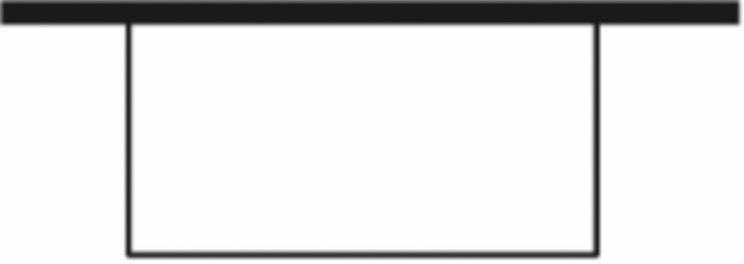
\includegraphics[width=0.28\textwidth]{figures/gao92_q8_fence.png}
\end{center}

\ifanswer
\solbegin
\step{设矩形的长为 $x$ 米，宽为 $y$，则 $xy=18$，}
\step{需要用栅栏长为 $x+2y\geqslant2\sqrt{2xy}=12$，}
\step{当且仅当 $x=2y$，即 $y=3$，$x=6$ 时取等号，故至少需要 $12$ 米栅栏.}
\solend
\fi

\item 已知 $a$ 为正整数，若关于 $x$ 的不等式 $\lvert x-2025\rvert\leqslant a$ 的解集中有且仅有 $7$ 个整数，则 $a$ 的值为\blankline[4.4em].

\ifanswer
\solbegin
\step{不等式 $\lvert x-2025\rvert\leqslant a$，则 $-a\leqslant x-2025\leqslant a$，即 $2025-a\leqslant x\leqslant2025+a$，}
\step{所以不等式 $\lvert x-2025\rvert\leqslant a$ 的解集为 $\{x\mid2025-a\leqslant x\leqslant2025+a\}$，}
\step{若不等式解集中有且仅有 $7$ 个整数，且 $a$ 为正整数，}
\step{由解集的对称性得这 $7$ 个整数以 $2025$ 为中心，向左右两边各延伸 $3$ 个整数，}
\step{即这 $7$ 个整数为 $2022,2023,2024,2025,2026,2027,2028$，所以 $a=3$.}
\solend
\fi

\item 已知关于 $x$ 的一元二次方程 $x^2-x+a=0$ 有两个不相等的正根 $m$、$n$，则 $\dfrac1m+\dfrac9n$ 的最小值为\blankline[4.4em].

\ifanswer
\solbegin
\step{因为一元二次方程 $x^2-x+a=0$ 有两个不相等的正根 $m$、$n$，}
\step{所以判别式 $\Delta=(-1)^2-4a>0\Rightarrow a<\dfrac14$，$m+n=1$，$mn=a>0$，}
\step{因此 $0<a<\dfrac14$ 且 $m+n=1(m,n>0)$.}
\step{$\dfrac1m+\dfrac9n=\left(\dfrac1m+\dfrac9n\right)(m+n)=1+\dfrac nm+\dfrac{9m}{n}+9=10+\dfrac nm+\dfrac{9m}{n}\geqslant10+2\sqrt9=16$，}
\step{等号成立条件为 $\dfrac nm=\dfrac{9m}{n}\Rightarrow n^2=9m^2\Rightarrow n=3m$，}
\step{$m$、$n>0$，结合 $m+n=1$，代入 $n=3m$ 得 $m+3m=1\Rightarrow m=\dfrac14$，$n=\dfrac34$，}
\step{此时 $mn=\dfrac14\cdot\dfrac34=\dfrac3{16}$，满足 $0<a<\dfrac14$，等号可取，因此 $\dfrac1m+\dfrac9n$ 的最小值为 $16$.}
\solend
\fi

\item 对任意 $A$、$B\subseteq R$，记 $A\oplus B=\{x\mid x\in A\cup B,x\notin A\cap B\}$，并称 $A\oplus B$ 为集合 $A$，$B$ 的对称差. 例如：若 $A=\{1,2,3\},B=\{2,3,4\}$，则 $A\oplus B=\{1,4\}$. 下列命题中，为真命题的有\blankline[4.4em].

①若 $A$、$B\subseteq R$ 且 $A\oplus B\subseteq A$，则 $A\subseteq B$

②若 $A$、$B\subseteq R$ 且 $A\oplus B=\varnothing$，则 $A=B$

③若 $A$、$B\subseteq R$ 且 $A\oplus B=B$，则 $A=\varnothing$

④对任意 $A$、$B\subseteq R$，都有 $A\oplus B=\complement_{R}A\oplus\complement_{R}B$

\ifanswer
\solbegin
\step{对于①，因为 $A\oplus B\subseteq A$，所以 $\{x\mid x\in A\cup B,x\notin A\cap B\}\subseteq A$，故 $B\subseteq A$，}
\step{故①错误；}
\step{对于②，$A$、$B\subseteq R$ 且 $A\oplus B=\varnothing$，则 $\varnothing=\{x\mid x\in A\cup B,x\notin A\cap B\}$，}
\step{即 $A\cup B=A\cap B$，所以 $A=B$，故②正确；}
\step{对于③，$A$、$B\subseteq R$ 且 $A\oplus B=B$，则 $B=\{x\mid x\in A\cup B,x\notin A\cap B\}$，}
\step{故 $A\subseteq B$，且 $B$ 中元素不在 $A\cap B$ 中，故 $A=\varnothing$，故③正确；}
\step{对于④，$\complement_{R}A\oplus\complement_{R}B=\{x\mid x\in\complement_{R}A\cup\complement_{R}B,x\notin\complement_{R}A\cap\complement_{R}B\}$，}
\step{其中 $\complement_{R}A\cup\complement_{R}B=\complement_{R}(A\cap B)$，$\complement_{R}A\cap\complement_{R}B=\complement_{R}(A\cup B)$，}
\step{故 $\complement_{R}A\oplus\complement_{R}B=\{x\mid x\in\complement_{R}(A\cap B)$，}
\step{$x\notin\complement_{R}(A\cup B)\}=\{x\mid x\in A\cup B,x\notin A\cap B\}$，}
\step{而 $A\oplus B=\{x\mid x\in A\cup B,x\notin A\cap B\}$，故 $A\oplus B=\complement_{R}A\oplus\complement_{R}B$，故④正确.}
\step{故正确的是②③④.}
\solend
\fi

\item 若不等式 $x^2-2ax+a^2-1\geqslant0$ 对任意 $x\in[0,2]$ 恒成立，则实数 $a$ 的取值范围是\blankline[4.4em].

\ifanswer
\solbegin
\step{由题意不等式 $x^2-2ax+a^2-1\geqslant0$ 对任意 $x\in[0,2]$ 恒成立，}
\step{解得 $x\leqslant a-1$ 或 $x\geqslant a+1$，要使此不等式对任意 $x\in[0,2]$ 恒成立，}
\step{则区间 $[0,2]$ 必须完全包含在解集 $(-\infty,a-1]\cup[a+1,+\infty)$ 中，}
\step{等价于 $[0,2]$ 与开区间 $(a-1,a+1)$ 的交集为空集，}
\step{区间 $[0,2]$ 在 $a-1$ 左侧，即 $2\leqslant a-1$，解得 $a\geqslant3$，}
\step{区间 $[0,2]$ 在 $a+1$ 右侧，即 $a+1\leqslant0$，解得 $a\leqslant-1$，}
\step{当 $a\in(-1,3)$，则 $(a-1,a+1)$ 与 $[0,2]$ 必有交集，不满足条件，}
\step{综上，实数 $a$ 的取值范围是 $(-\infty,-1]\cup[3,+\infty)$.}
\solend
\fi

\end{enumerate}

\bigsec{二、选择题}

\begin{enumerate}
\setcounter{enumi}{12}

\item 若 $a<b<0$，则下列不等式成立的是\mbox{（\quad）}% 原卷括号内已印“D”，试卷版按惯例留空

\keepwithprev
A. $a^2<b^2$\qquad B. $\dfrac1a<\dfrac1b$\qquad C. $ab<b^2$\qquad D. $ab<a^2$

\ifanswer
\ans{$D$}
\fi

\item 已知全集 $U=\{1,2,3,4,5\}$，集合 $A,B$ 是 $U$ 子集，满足 $\overline{A\cup B}=\{4,5\}$，$B=\{2,3\}$，则 $A\cap\overline B=\mbox{（\quad）}$

\keepwithprev
A. $\{1\}$\qquad B. $\{1,2\}$\qquad C. $\{1,4,5\}$\qquad D. $\varnothing$

\ifanswer
\solbegin
\step{因为全集 $U=\{1,2,3,4,5\}$，集合 $A$、$B$ 是 $U$ 子集，$\overline{A\cup B}=\{4,5\}$，$B=\{2,3\}$，}
\step{所以 $A\cup B=\{1,2,3\}$，故 $1\in A$，$1\notin B$，$4\notin A$，$5\notin A$，$4\notin B$，$5\notin B$，}
\step{故 $A\cap\overline B=\{1\}$. 故选 $A$.}
\solend
\fi

\item 设 $a>0$，若关于 $x$ 的不等式 $x^2-(2a-1)x-2a<0$ 的解集中恰有 $3$ 个整数，则实数 $a$ 的取值范围是\mbox{（\quad）}

\keepwithprev
A. $\left[1,\dfrac32\right]$\qquad B. $\left(1,\dfrac32\right]$\qquad C. $\left[\dfrac12,1\right]$\qquad D. $\left(\dfrac12,1\right]$

\ifanswer
\solbegin
\step{已知关于 $x$ 的不等式 $x^2-(2a-1)x-2a<0$，则 $(x+1)(x-2a)<0$，}
\step{则 $-1<x<2a$，又解集中恰有 $3$ 个整数，则 $2<2a\leqslant3$，则 $1<a\leqslant\dfrac32$，}
\step{则 $a$ 的取值范围为 $\left(1,\dfrac32\right]$. 故选 $B$.}
\solend
\fi

\item 已知集合 $U=\{1,2,3,\cdots,2027\}$，$M\subseteq U$，若对于 $M$ 中的任意两个不同的元素 $x$、$y$，都有 $\lvert x-y\rvert>2$，则 $M$ 中元素个数的最大值为\mbox{（\quad）}

\keepwithprev
A. $675$\qquad B. $676$\qquad C. $2025$\qquad D. $2026$

\ifanswer
\solbegin
\step{对于 $M$ 中的任意两个不同的元素 $x$、$y$，都有 $\lvert x-y\rvert>2$，}
\step{不妨设 $x>y$，都有 $x-y\geqslant3$，}
\step{要想 $M$ 所含元素个数最大，则要 $x-y$ 尽可能小，故需使得 $x-y$ 的最小值为 $3$，}
\step{将 $1\sim2027$ 这 $2027$ 个元素按如下分组：}
\step{$\{1,2,3\},\{4,5,6\},\cdots,\{2023,2024,2025\},\{2026,2027\}$，}
\step{故应在前 $675$ 组中按周期 $3$ 每组取一个元素，且第一组中不能取 $3$，}
\step{第一组中取 $1$ 时，得 $M=\{1,4,7,\cdots,2023,2026\}$}
\step{或 $M=\{1,4,7,\cdots,2023,2027\}$ 这样的集合，}
\step{第一组取 $2$ 时，得 $M=\{2,5,8,\cdots,2024,2027\}$，}
\step{其中任意两元素差值 $x-y(x>y)$ 都大于 $2$，满足题意，}
\step{故 $M$ 所含元素个数的最大值为 $\dfrac{2025}{3}+1=676$. 故选 $B$.}
\solend
\fi

\end{enumerate}

\bigsec{三、解答题}

\begin{enumerate}
\setcounter{enumi}{16}

\item 已知集合 $M=\{x\mid a-1\leqslant x\leqslant2a+3\}$，$P=\{x\mid-2<x\leqslant4\}$，全集 $U=R$.

（1）当 $a=2$ 时，求 $M\cap P$；

（2）若 $x\in P$ 是 $x\in M$ 的必要不充分条件，求实数 $a$ 的取值范围.

\ansspace*[9]

\ifanswer
\solbegin
\stepm{（1）}{当 $a=2$ 时，集合 $M=\{x\mid1\leqslant x\leqslant7\}$，所以 $M\cap P=\{x\mid1\leqslant x\leqslant4\}$；}
\stepm{（2）}{因为 $x\in P$ 是 $x\in M$ 的必要不充分条件，所以 $M\subsetneqq P$，}
\step{当 $M=\varnothing$ 时，$a-1>2a+3$，解得 $a<-4$，}
\step{当 $M\neq\varnothing$ 时，则 $\begin{cases}a-1\leqslant2a+3\\ a-1>-2\\ 2a+3\leqslant4\end{cases}$，解得 $-1<a\leqslant\dfrac12$，}
\step{综上所述，实数 $a$ 的取值范围为 $(-\infty,-4)\cup\left(-1,\dfrac12\right]$.}
\solend
\fi

\item 命题甲：关于 $x$ 的方程 $(a-1)x^2+(2a-4)x+a=0$ 有两个不相等的实数根；

命题乙：关于 $x$ 的不等式 $ax^2-2ax+a+1>0$ 的解集为 $R$.

（1）若命题甲为真命题，求实数 $a$ 的取值范围；

（2）若命题甲、乙中至多有一个为真命题，求实数 $a$ 的取值范围.

\ansspace*[12]

\ifanswer
\solbegin
\stepm{（1）}{命题甲：关于 $x$ 的方程 $(a-1)x^2+(2a-4)x+a=0$ 有两个不相等的实数根，}
\step{则 $\begin{cases}a-1\neq0\\ \Delta=(2a-4)^2-4a(a-1)>0\end{cases}$，解得 $a<\dfrac43$ 且 $a\neq1$，}
\step{故 $a$ 的范围为 $\left\{a\left|a<\dfrac43\ \text{且}\ a\neq1\right.\right\}$；}
\stepm{（2）}{当 $a=0$ 时 $y=1>0$，符合题意；}
\step{当 $a\neq0$，由 $\begin{cases}a>0\\ \Delta=4a^2-4a(a+1)<0\end{cases}$，解得 $a>0$，}
\step{则 $a$ 的取值范围为 $a\geqslant0$，}
\step{故 $p$、$q$ 都为真时，$a$ 的范围为 $0\leqslant a<\dfrac43$ 且 $a\neq1$，}
\step{则命题甲、乙中至多有一个为真命题时，}
\step{$a$ 的取值范围为 $\left\{a\left|a<0\ \text{或}\ a=1\ \text{或}\ a\geqslant\dfrac43\right.\right\}$.}
\solend
\fi

\item 如图，$OA$、$OB$ 是两条长度足够长的互相垂直的笔直小路，矩形 $OCPD$ 的顶点 $C$，$D$ 分别在 $OA$、$OB$ 上，且该矩形区域内种满了荷花. 为了让观赏者有更好的观赏体验，现计划经过点 $P$ 修一条小路 $EF$，其中点 $E$ 在小路 $OA$ 上，点 $F$ 在小路 $OB$ 上，并在 $\triangle OEF$ 区域内种满荷花. 已知 $OD=25$ m，$OC=40$ m，且小路 $EF$ 要完全位于一个以 $O$ 为顶点的，边长为 $100$ m 的正方形内部（包括边界）. 记 $\triangle OEF$ 的面积为 $S$ m$^2$.

\begin{center}
\begin{tikzpicture}[x=0.46cm,y=0.42cm,line width=0.7pt]
\draw (0,0) -- (0,10.2) node[above,inner sep=3pt] {$A$};
\draw (0,0) -- (11.8,0) node[right,inner sep=3pt] {$B$};
\draw (0,4.83) -- (2.42,4.83) -- (2.42,0);
\draw (0,6.92) -- (8.01,0);
\node[below left,inner sep=2pt] at (0,0) {$O$};
\node[below,inner sep=2pt] at (2.42,0) {$D$};
\node[left,inner sep=3pt] at (0,4.83) {$C$};
\node[above right,inner sep=1pt] at (2.42,4.83) {$P$};
\node[left,inner sep=3pt] at (0,6.92) {$E$};
\node[below,inner sep=2pt] at (8.01,0) {$F$};
\end{tikzpicture}
\end{center}

（1）设 $EC=x\cdot m$，试用 $x$ 表示 $OF$，并求 $x$ 的取值范围.

（2）当 $EC$ 的长度为多少时，$S$ 取得最小值？最小值是多少？

\ansspace*[11]

\ifanswer
\solbegin
\stepm{（1）}{由题意得 $x\leqslant60$，}
\step{$\triangle PCE\backsim\triangle FDP$，所以 $\dfrac{EC}{CP}=\dfrac{PD}{DF}$，即 $\dfrac{x}{25}=\dfrac{40}{DF}$，得 $DF=\dfrac{1000}{x}$ m，}
\step{所以 $OF=OD+DF=\left(25+\dfrac{1000}{x}\right)$ m，}
\step{所以 $25+\dfrac{1000}{x}\leqslant100$，解得 $x\geqslant\dfrac{40}{3}$；}
\step{综上，$\dfrac{40}{3}\leqslant x\leqslant60$；}
\stepm{（2）}{由 $OE=OC+CE=(40+x)$ m，}
\step{所以 $S=\dfrac12\cdot OF\cdot OE=\dfrac12\left(25+\dfrac{1000}{x}\right)(40+x)$}
\step{$=\dfrac12\left(1000+25x+\dfrac{40000}{x}+1000\right)$ m$^2$，}
\step{由基本不等式得 $S\geqslant\dfrac12\left(2000+2\sqrt{25x\cdot\dfrac{40000}{x}}\right)=2000$ m$^2$，}
\step{当且仅当 $25x=\dfrac{40000}{x}$，即 $x=40$ 时取等号，}
\step{故 $EC=40$ m 时，$S$ 取得最小值，为 $2000$ m$^2$.}
\solend
\fi

\item 已知函数 $f(x)=x^2-(a-2)x+a-3$.

（1）若 $f(x)=0$ 的两根为 $\alpha,\beta$，$\alpha^2+\beta^2=2$，求 $a$ 的值；

（2）解关于 $x$ 的不等式 $f(x)\geqslant0$；

（3）是否存在整数 $m,n$，使得关于 $x$ 的不等式 $m\leqslant f(x)\leqslant n$ 的解集恰好为 $[m,n]$？若存在，求出 $m,n$ 的值. 若不存在，请说明理由.

\ansspace*[16]

\ifanswer
\solbegin
\stepm{（1）}{由韦达定理，$\alpha+\beta=a-2,\alpha\beta=a-3$，}
\step{因此 $\alpha^2+\beta^2=(a-2)^2-2(a-3)=2\Leftrightarrow(a-2)(a-4)=0$，}
\step{$a=2$ 时两根为 $1,-1$；$a=4$ 时两根均为 $1$，均满足条件，}
\step{所以 $a=2$ 或 $a=4$.}
\stepm{（2）}{因为 $f(x)=(x-1)[x-(a-3)]$，所以分三种情况：}
\step{当 $a<4$ 时，$a-3<1$，解集为 $(-\infty,a-3]\cup[1,+\infty)$.}
\step{当 $a=4$ 时，$f(x)=(x-1)^2\geqslant0$ 恒成立，解集为 $R$.}
\step{当 $a>4$ 时，$a-3>1$，解集为 $(-\infty,1]\cup[a-3,+\infty)$.}
\stepm{（3）}{区间 $[m,n]$ 要求 $m<n$. 记 $f(x)$ 的最小值为 $k$.}
\step{$[m,n]$ 非空，不等式 $f(x)\leqslant n$ 有解，其解集为闭区间 $[x_1,x_2]$，}
\step{其中 $x_1\leqslant x_2$ 是方程 $f(x)=n$ 的两根.}
\step{若 $k<m$，则 $f(x)<m$ 的解集是 $[x_1,x_2]$ 内部的一个开区间，}
\step{从 $[x_1,x_2]$ 中去掉它后剩下两段，原不等式的解集不是一个区间，矛盾，}
\step{所以 $k\geqslant m$，原不等式的解集就是 $[x_1,x_2]$，于是 $m=x_1,n=x_2$，}
\step{即 $f(m)=f(n)=n$，于是 $f(m)-f(n)=(m-n)(m+n-a+2)=0$.}
\step{因为 $m\neq n$，所以 $a=m+n+2$.}
\step{代入 $f(m)=n$，得 $(m-1)(1-n)=n\Leftrightarrow m(n-1)=-1$，$m,n$ 均为整数，}
\step{因此 $(m,n)=(-1,2)$ 或 $(m,n)=(1,0)$.}
\step{结合 $m<n$，只可能有 $m=-1,n=2$，此时 $a=3$.}
\step{检验：此时 $f(x)=x^2-x$，且 $x^2-x=\left(x-\dfrac12\right)^2-\dfrac14\geqslant-\dfrac14>-1$，}
\step{因此 $-1\leqslant f(x)\leqslant2\Leftrightarrow x^2-x\leqslant2\Leftrightarrow(x+1)(x-2)\leqslant0\Leftrightarrow x\in[-1,2]$，}
\step{所以存在符合条件的整数 $m=-1,n=2$.}
\solend
\fi

\item 给定数集 $M$，若对于任意 $a$、$b\in M$，有 $a+b\in M,a-b\in M$，则称集合 $M$ 为闭集合.

（1）判断集合 $A_1=\{-4,-2,0,2,4\}$，集合 $B=\{x\mid x=3k,k\in\Z\}$ 是否为闭集合；

（2）若集合 $C$、$D$ 为闭集合，则 $C\cup D$ 是否一定为闭集合？请说明理由；

（3）已知集合 $C$、$D$ 为闭集合，且 $C\subsetneq R,D\subsetneq R$，证明：$(C\cup D)\subsetneq R$.% 原卷印作 (C∪D)⊂R，按解析证明的是 C∪D≠R，排真子集

\ansspace*[14]

\ifanswer
\solbegin
\stepm{（1）}{因为 $4\in A_1$，$2\in A_1$，$4+2=6\notin A_1$，所以 $A_1$ 不是闭集合；}
\step{任取 $x,y\in B$，设 $x=3m,y=3n,m,n\in\Z$，}
\step{则 $x+y=3m+3n=3(m+n)$ 且 $m+n\in\Z$，}
\step{所以 $x+y\in B$，同理，$x-y\in B$，故 $B$ 为闭集合.}
\stepm{（2）}{结论：不一定.}
\step{不妨令 $C=\{x\mid x=2k,k\in\Z\},D=\{x\mid x=3k,k\in\Z\}$，}
\step{则由（1）得 $C$、$D$ 为闭集合，易得 $2,3\in C\cup D,2+3=5\notin C\cup D$，}
\step{因此，$C\cup D$ 不一定是闭集合.}
\stepm{（3）}{不妨假设 $C\cup D=R$，则由 $C\subsetneq R$，得存在 $a\in R$ 且 $a\notin C$，故 $a\in D$.}
\step{同理，存在 $b\in R$ 且 $b\notin D$，故 $b\in C$.}
\step{因为 $a+b\in R=C\cup D$，所以 $a+b\in C$ 或 $a+b\in D$.}
\step{若 $a+b\in C$，则由 $C$ 为闭集合且 $b\in C$，得 $a=(a+b)-b\in C$，}
\step{与 $a\notin C$ 矛盾.}
\step{若 $a+b\in D$，则由 $D$ 为闭集合且 $a\in D$，得 $b=(a+b)-a\in D$，}
\step{与 $b\notin D$ 矛盾.}
\step{综上，$C\cup D=R$ 不成立，故 $(C\cup D)\subsetneq R$.}
\solend
\fi

\end{enumerate}

\end{document}
"
%
% 原始材料：微信公众号“魔都数学加油站”文章，连载“27学年高一92”；
% 原文标题“27学年高一92——2026-2027年上海市闵行实验高一上10月月考”；
% 原文链接：https://mp.weixin.qq.com/s/8HUyr3G7GpcHyczwu_XYCQ。
% 正文为 10 张 PNG 页（`原图/高一92_闵行实验_10月月考/01..10.png`），均 4762×6735，按页序读取。
%
% 篇幅与题号：原卷自第 3 题起编号（第 1、2 题不在原文内）。填空题 3—12（10 题）、
% 选择题 13—16（4 题）、解答题 17—21（5 题），共 19 题。
%
% 讲评版：第 6 题只印【答案】（“$[-1,3]$”），本稿只给 \ans{}；第 13 题无【解析】、
% 答案“D”直接印在题干括号内，本稿试卷版按惯例留空、答案版提 \ans{$D$}；其余 17 题印
% 【解析】，其中选择题答案在解析末句“故选 $A$／$B$／$B$”。
% 第 8 题题干右侧有一幅“围墙 + 三面栅栏”示意图（裁自第 2 页原图）；第 19 题题干带
% 与 高一88 第 19 题同型的示意图（$OA$／$OB$ 两条小路、矩形 $OCPD$、折线 $EF$），用 TikZ 重绘。
%
% 副标题：原卷未印副标题。本稿按内容标作“集合与常用逻辑用语、不等式”。
%
% 原卷笔误/存疑（均照录未改，正文对应处另有 % 注）：
%   ① 第 21 题 (3) 题干与解析末句把结论印作“$(C\cup D)\subset R$”，而解析证明的是
%      “$C\cup D=\R$ 不成立”，按文意应为“$(C\cup D)\subsetneq\R$”；本稿按真子集排
%      $\subsetneq$，原卷记号照录于文件头；
%   ② 第 7 题解析只列 $B=\varnothing$（$a=0$）、$B=\{1\}$（$a=1$）、$B=\{-3\}$（$a=-\frac13$）
%      三种情形，与结论 $\left\{0,1,-\frac13\right\}$ 相符，无笔误。
%
% 与原卷的排版差异：
%   ① 原卷每题下直接印【答案】/【解析】，本稿按全稿惯例将答案与解析置于答案版；
%   ② 原卷未印副标题，本稿补出；填空横线统一排 \blankline[4.4em]；
%   ③ 原卷数集记号排斜体 $R$、$Z$，本稿按全稿惯例改用 $\R$、$\Z$；
%   ④ 第 17—21 题的子问用行内“（1）（2）（3）”段，解析中的子问标号用 \stepm；
%   ⑤ 解答题按惯例加 \ansspace；选择题括号排 \mbox{（\quad）}；
%   ⑥ 第 8 题的示意图原卷排在题干右侧、文字绕排，本稿改排为题干后的居中图
%      （自原图裁切、去粉色水印后转灰度）；第 19 题的图按原图比例 TikZ 重绘。
%
% 行数核对：逐题数 \step/\stepm 条数，合计 128 条（Q3：2；Q4：3；Q5：2；Q6：0；Q7：6；
% Q8：3；Q9：5；Q10：7；Q11：12；Q12：8；Q13：0；Q14：3；Q15：3；Q16：11；Q17：5；
% Q18：9；Q19：11；Q20：22；Q21：16）。第 6 题只印答案、第 13 题无解析，均不计入 \step 账。
% 原卷解析的换行按语意合并，未逐行强拆。
%
\documentclass[a4paper,11pt]{article}
\usepackage{common}

\begin{document}

\examtitlest[7]{2026--2027 年闵行实验高一上 10 月月考}{集合与常用逻辑用语、不等式}

\bigsec{一、填空题}

\begin{enumerate}
\setcounter{enumi}{2}

\item 已知 $3<a<8$，$4<b<9$，则 $\dfrac ab$ 的取值范围是\blankline[4.4em].

\ifanswer
\solbegin
\step{因为 $4<b<9$，所以 $\dfrac19<\dfrac1b<\dfrac14$，又 $3<a<8$，所以 $\dfrac13<\dfrac ab<2$，}
\step{故 $\dfrac ab$ 的取值范围是 $\left(\dfrac13,2\right)$.}
\solend
\fi

\item 已知 $p:x>3$，$q:x>5$，则 $p$ 是 $q$ 的\blankline[4.4em]（选“充分不必要条件”“必要不充分条件”“充要条件”“既不充分也不必要条件”之一填空）.

\ifanswer
\solbegin
\step{当 $x>3$ 时，不能推出 $x>5$，充分性不成立；}
\step{当 $x>5$ 时，可以得到 $x>3$，必要性成立；}
\step{故 $p$ 是 $q$ 的必要不充分条件.}
\solend
\fi

\item 不等式 $\dfrac{x-1}{2x+1}\leqslant1$ 的解集为\blankline[4.4em].

\ifanswer
\solbegin
\step{因为 $\dfrac{x-1}{2x+1}\leqslant1$，所以 $\dfrac{x-1}{2x+1}-\dfrac{2x+1}{2x+1}\leqslant0$，所以 $\dfrac{x+2}{2x+1}\geqslant0$，}
\step{所以 $x>-\dfrac12$ 或 $x\leqslant-2$，即不等式的解集是 $(-\infty,-2]\cup\left(-\dfrac12,+\infty\right)$.}
\solend
\fi

\item 设 $x\in R$，则方程 $\lvert x+1\rvert+\lvert x-3\rvert=4$ 的解集为\blankline[4.4em].

\ifanswer
\ans{$[-1,3]$}
\fi

\item 若 $A=\{x\mid x^2+2x=3\}$，$B=\{x\mid ax=1\}$，且 $B\subseteq A$，则实数 $a$ 的值组成的集合为\blankline[4.4em].

\ifanswer
\solbegin
\step{由 $x^2+2x=3$ 得 $x^2+2x-3=0$，解得 $x=1$ 或 $x=-3$，所以 $A=\{1,-3\}$，}
\step{又因为 $B=\{x\mid ax=1\}$，且 $B\subseteq A$，}
\step{当 $B=\varnothing$，即 $a=0$ 时，显然符合题意；}
\step{当 $B=\{1\}$，即 $a=1$ 时，也符合题意；}
\step{当 $B=\{-3\}$，即 $a=-\dfrac13$ 时，也符合题意；}
\step{综上所述，实数 $a$ 的值组成的集合为 $\left\{0,1,-\dfrac13\right\}$.}
\solend
\fi

\item 某校欲在围墙边用栅栏围成一个 $18$ 平方米的矩形区域，作为天鹅的地面栖息地，矩形区域的一条边为围墙（如图），则至少需要\blankline[4.4em]米栅栏.

\begin{center}
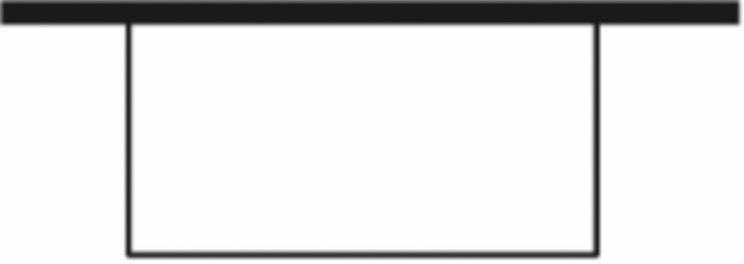
\includegraphics[width=0.28\textwidth]{figures/gao92_q8_fence.png}
\end{center}

\ifanswer
\solbegin
\step{设矩形的长为 $x$ 米，宽为 $y$，则 $xy=18$，}
\step{需要用栅栏长为 $x+2y\geqslant2\sqrt{2xy}=12$，}
\step{当且仅当 $x=2y$，即 $y=3$，$x=6$ 时取等号，故至少需要 $12$ 米栅栏.}
\solend
\fi

\item 已知 $a$ 为正整数，若关于 $x$ 的不等式 $\lvert x-2025\rvert\leqslant a$ 的解集中有且仅有 $7$ 个整数，则 $a$ 的值为\blankline[4.4em].

\ifanswer
\solbegin
\step{不等式 $\lvert x-2025\rvert\leqslant a$，则 $-a\leqslant x-2025\leqslant a$，即 $2025-a\leqslant x\leqslant2025+a$，}
\step{所以不等式 $\lvert x-2025\rvert\leqslant a$ 的解集为 $\{x\mid2025-a\leqslant x\leqslant2025+a\}$，}
\step{若不等式解集中有且仅有 $7$ 个整数，且 $a$ 为正整数，}
\step{由解集的对称性得这 $7$ 个整数以 $2025$ 为中心，向左右两边各延伸 $3$ 个整数，}
\step{即这 $7$ 个整数为 $2022,2023,2024,2025,2026,2027,2028$，所以 $a=3$.}
\solend
\fi

\item 已知关于 $x$ 的一元二次方程 $x^2-x+a=0$ 有两个不相等的正根 $m$、$n$，则 $\dfrac1m+\dfrac9n$ 的最小值为\blankline[4.4em].

\ifanswer
\solbegin
\step{因为一元二次方程 $x^2-x+a=0$ 有两个不相等的正根 $m$、$n$，}
\step{所以判别式 $\Delta=(-1)^2-4a>0\Rightarrow a<\dfrac14$，$m+n=1$，$mn=a>0$，}
\step{因此 $0<a<\dfrac14$ 且 $m+n=1(m,n>0)$.}
\step{$\dfrac1m+\dfrac9n=\left(\dfrac1m+\dfrac9n\right)(m+n)=1+\dfrac nm+\dfrac{9m}{n}+9=10+\dfrac nm+\dfrac{9m}{n}\geqslant10+2\sqrt9=16$，}
\step{等号成立条件为 $\dfrac nm=\dfrac{9m}{n}\Rightarrow n^2=9m^2\Rightarrow n=3m$，}
\step{$m$、$n>0$，结合 $m+n=1$，代入 $n=3m$ 得 $m+3m=1\Rightarrow m=\dfrac14$，$n=\dfrac34$，}
\step{此时 $mn=\dfrac14\cdot\dfrac34=\dfrac3{16}$，满足 $0<a<\dfrac14$，等号可取，因此 $\dfrac1m+\dfrac9n$ 的最小值为 $16$.}
\solend
\fi

\item 对任意 $A$、$B\subseteq R$，记 $A\oplus B=\{x\mid x\in A\cup B,x\notin A\cap B\}$，并称 $A\oplus B$ 为集合 $A$，$B$ 的对称差. 例如：若 $A=\{1,2,3\},B=\{2,3,4\}$，则 $A\oplus B=\{1,4\}$. 下列命题中，为真命题的有\blankline[4.4em].

①若 $A$、$B\subseteq R$ 且 $A\oplus B\subseteq A$，则 $A\subseteq B$

②若 $A$、$B\subseteq R$ 且 $A\oplus B=\varnothing$，则 $A=B$

③若 $A$、$B\subseteq R$ 且 $A\oplus B=B$，则 $A=\varnothing$

④对任意 $A$、$B\subseteq R$，都有 $A\oplus B=\complement_{R}A\oplus\complement_{R}B$

\ifanswer
\solbegin
\step{对于①，因为 $A\oplus B\subseteq A$，所以 $\{x\mid x\in A\cup B,x\notin A\cap B\}\subseteq A$，故 $B\subseteq A$，}
\step{故①错误；}
\step{对于②，$A$、$B\subseteq R$ 且 $A\oplus B=\varnothing$，则 $\varnothing=\{x\mid x\in A\cup B,x\notin A\cap B\}$，}
\step{即 $A\cup B=A\cap B$，所以 $A=B$，故②正确；}
\step{对于③，$A$、$B\subseteq R$ 且 $A\oplus B=B$，则 $B=\{x\mid x\in A\cup B,x\notin A\cap B\}$，}
\step{故 $A\subseteq B$，且 $B$ 中元素不在 $A\cap B$ 中，故 $A=\varnothing$，故③正确；}
\step{对于④，$\complement_{R}A\oplus\complement_{R}B=\{x\mid x\in\complement_{R}A\cup\complement_{R}B,x\notin\complement_{R}A\cap\complement_{R}B\}$，}
\step{其中 $\complement_{R}A\cup\complement_{R}B=\complement_{R}(A\cap B)$，$\complement_{R}A\cap\complement_{R}B=\complement_{R}(A\cup B)$，}
\step{故 $\complement_{R}A\oplus\complement_{R}B=\{x\mid x\in\complement_{R}(A\cap B)$，}
\step{$x\notin\complement_{R}(A\cup B)\}=\{x\mid x\in A\cup B,x\notin A\cap B\}$，}
\step{而 $A\oplus B=\{x\mid x\in A\cup B,x\notin A\cap B\}$，故 $A\oplus B=\complement_{R}A\oplus\complement_{R}B$，故④正确.}
\step{故正确的是②③④.}
\solend
\fi

\item 若不等式 $x^2-2ax+a^2-1\geqslant0$ 对任意 $x\in[0,2]$ 恒成立，则实数 $a$ 的取值范围是\blankline[4.4em].

\ifanswer
\solbegin
\step{由题意不等式 $x^2-2ax+a^2-1\geqslant0$ 对任意 $x\in[0,2]$ 恒成立，}
\step{解得 $x\leqslant a-1$ 或 $x\geqslant a+1$，要使此不等式对任意 $x\in[0,2]$ 恒成立，}
\step{则区间 $[0,2]$ 必须完全包含在解集 $(-\infty,a-1]\cup[a+1,+\infty)$ 中，}
\step{等价于 $[0,2]$ 与开区间 $(a-1,a+1)$ 的交集为空集，}
\step{区间 $[0,2]$ 在 $a-1$ 左侧，即 $2\leqslant a-1$，解得 $a\geqslant3$，}
\step{区间 $[0,2]$ 在 $a+1$ 右侧，即 $a+1\leqslant0$，解得 $a\leqslant-1$，}
\step{当 $a\in(-1,3)$，则 $(a-1,a+1)$ 与 $[0,2]$ 必有交集，不满足条件，}
\step{综上，实数 $a$ 的取值范围是 $(-\infty,-1]\cup[3,+\infty)$.}
\solend
\fi

\end{enumerate}

\bigsec{二、选择题}

\begin{enumerate}
\setcounter{enumi}{12}

\item 若 $a<b<0$，则下列不等式成立的是\mbox{（\quad）}% 原卷括号内已印“D”，试卷版按惯例留空

\keepwithprev
A. $a^2<b^2$\qquad B. $\dfrac1a<\dfrac1b$\qquad C. $ab<b^2$\qquad D. $ab<a^2$

\ifanswer
\ans{$D$}
\fi

\item 已知全集 $U=\{1,2,3,4,5\}$，集合 $A,B$ 是 $U$ 子集，满足 $\overline{A\cup B}=\{4,5\}$，$B=\{2,3\}$，则 $A\cap\overline B=\mbox{（\quad）}$

\keepwithprev
A. $\{1\}$\qquad B. $\{1,2\}$\qquad C. $\{1,4,5\}$\qquad D. $\varnothing$

\ifanswer
\solbegin
\step{因为全集 $U=\{1,2,3,4,5\}$，集合 $A$、$B$ 是 $U$ 子集，$\overline{A\cup B}=\{4,5\}$，$B=\{2,3\}$，}
\step{所以 $A\cup B=\{1,2,3\}$，故 $1\in A$，$1\notin B$，$4\notin A$，$5\notin A$，$4\notin B$，$5\notin B$，}
\step{故 $A\cap\overline B=\{1\}$. 故选 $A$.}
\solend
\fi

\item 设 $a>0$，若关于 $x$ 的不等式 $x^2-(2a-1)x-2a<0$ 的解集中恰有 $3$ 个整数，则实数 $a$ 的取值范围是\mbox{（\quad）}

\keepwithprev
A. $\left[1,\dfrac32\right]$\qquad B. $\left(1,\dfrac32\right]$\qquad C. $\left[\dfrac12,1\right]$\qquad D. $\left(\dfrac12,1\right]$

\ifanswer
\solbegin
\step{已知关于 $x$ 的不等式 $x^2-(2a-1)x-2a<0$，则 $(x+1)(x-2a)<0$，}
\step{则 $-1<x<2a$，又解集中恰有 $3$ 个整数，则 $2<2a\leqslant3$，则 $1<a\leqslant\dfrac32$，}
\step{则 $a$ 的取值范围为 $\left(1,\dfrac32\right]$. 故选 $B$.}
\solend
\fi

\item 已知集合 $U=\{1,2,3,\cdots,2027\}$，$M\subseteq U$，若对于 $M$ 中的任意两个不同的元素 $x$、$y$，都有 $\lvert x-y\rvert>2$，则 $M$ 中元素个数的最大值为\mbox{（\quad）}

\keepwithprev
A. $675$\qquad B. $676$\qquad C. $2025$\qquad D. $2026$

\ifanswer
\solbegin
\step{对于 $M$ 中的任意两个不同的元素 $x$、$y$，都有 $\lvert x-y\rvert>2$，}
\step{不妨设 $x>y$，都有 $x-y\geqslant3$，}
\step{要想 $M$ 所含元素个数最大，则要 $x-y$ 尽可能小，故需使得 $x-y$ 的最小值为 $3$，}
\step{将 $1\sim2027$ 这 $2027$ 个元素按如下分组：}
\step{$\{1,2,3\},\{4,5,6\},\cdots,\{2023,2024,2025\},\{2026,2027\}$，}
\step{故应在前 $675$ 组中按周期 $3$ 每组取一个元素，且第一组中不能取 $3$，}
\step{第一组中取 $1$ 时，得 $M=\{1,4,7,\cdots,2023,2026\}$}
\step{或 $M=\{1,4,7,\cdots,2023,2027\}$ 这样的集合，}
\step{第一组取 $2$ 时，得 $M=\{2,5,8,\cdots,2024,2027\}$，}
\step{其中任意两元素差值 $x-y(x>y)$ 都大于 $2$，满足题意，}
\step{故 $M$ 所含元素个数的最大值为 $\dfrac{2025}{3}+1=676$. 故选 $B$.}
\solend
\fi

\end{enumerate}

\bigsec{三、解答题}

\begin{enumerate}
\setcounter{enumi}{16}

\item 已知集合 $M=\{x\mid a-1\leqslant x\leqslant2a+3\}$，$P=\{x\mid-2<x\leqslant4\}$，全集 $U=R$.

（1）当 $a=2$ 时，求 $M\cap P$；

（2）若 $x\in P$ 是 $x\in M$ 的必要不充分条件，求实数 $a$ 的取值范围.

\ansspace*[9]

\ifanswer
\solbegin
\stepm{（1）}{当 $a=2$ 时，集合 $M=\{x\mid1\leqslant x\leqslant7\}$，所以 $M\cap P=\{x\mid1\leqslant x\leqslant4\}$；}
\stepm{（2）}{因为 $x\in P$ 是 $x\in M$ 的必要不充分条件，所以 $M\subsetneqq P$，}
\step{当 $M=\varnothing$ 时，$a-1>2a+3$，解得 $a<-4$，}
\step{当 $M\neq\varnothing$ 时，则 $\begin{cases}a-1\leqslant2a+3\\ a-1>-2\\ 2a+3\leqslant4\end{cases}$，解得 $-1<a\leqslant\dfrac12$，}
\step{综上所述，实数 $a$ 的取值范围为 $(-\infty,-4)\cup\left(-1,\dfrac12\right]$.}
\solend
\fi

\item 命题甲：关于 $x$ 的方程 $(a-1)x^2+(2a-4)x+a=0$ 有两个不相等的实数根；

命题乙：关于 $x$ 的不等式 $ax^2-2ax+a+1>0$ 的解集为 $R$.

（1）若命题甲为真命题，求实数 $a$ 的取值范围；

（2）若命题甲、乙中至多有一个为真命题，求实数 $a$ 的取值范围.

\ansspace*[12]

\ifanswer
\solbegin
\stepm{（1）}{命题甲：关于 $x$ 的方程 $(a-1)x^2+(2a-4)x+a=0$ 有两个不相等的实数根，}
\step{则 $\begin{cases}a-1\neq0\\ \Delta=(2a-4)^2-4a(a-1)>0\end{cases}$，解得 $a<\dfrac43$ 且 $a\neq1$，}
\step{故 $a$ 的范围为 $\left\{a\left|a<\dfrac43\ \text{且}\ a\neq1\right.\right\}$；}
\stepm{（2）}{当 $a=0$ 时 $y=1>0$，符合题意；}
\step{当 $a\neq0$，由 $\begin{cases}a>0\\ \Delta=4a^2-4a(a+1)<0\end{cases}$，解得 $a>0$，}
\step{则 $a$ 的取值范围为 $a\geqslant0$，}
\step{故 $p$、$q$ 都为真时，$a$ 的范围为 $0\leqslant a<\dfrac43$ 且 $a\neq1$，}
\step{则命题甲、乙中至多有一个为真命题时，}
\step{$a$ 的取值范围为 $\left\{a\left|a<0\ \text{或}\ a=1\ \text{或}\ a\geqslant\dfrac43\right.\right\}$.}
\solend
\fi

\item 如图，$OA$、$OB$ 是两条长度足够长的互相垂直的笔直小路，矩形 $OCPD$ 的顶点 $C$，$D$ 分别在 $OA$、$OB$ 上，且该矩形区域内种满了荷花. 为了让观赏者有更好的观赏体验，现计划经过点 $P$ 修一条小路 $EF$，其中点 $E$ 在小路 $OA$ 上，点 $F$ 在小路 $OB$ 上，并在 $\triangle OEF$ 区域内种满荷花. 已知 $OD=25$ m，$OC=40$ m，且小路 $EF$ 要完全位于一个以 $O$ 为顶点的，边长为 $100$ m 的正方形内部（包括边界）. 记 $\triangle OEF$ 的面积为 $S$ m$^2$.

\begin{center}
\begin{tikzpicture}[x=0.46cm,y=0.42cm,line width=0.7pt]
\draw (0,0) -- (0,10.2) node[above,inner sep=3pt] {$A$};
\draw (0,0) -- (11.8,0) node[right,inner sep=3pt] {$B$};
\draw (0,4.83) -- (2.42,4.83) -- (2.42,0);
\draw (0,6.92) -- (8.01,0);
\node[below left,inner sep=2pt] at (0,0) {$O$};
\node[below,inner sep=2pt] at (2.42,0) {$D$};
\node[left,inner sep=3pt] at (0,4.83) {$C$};
\node[above right,inner sep=1pt] at (2.42,4.83) {$P$};
\node[left,inner sep=3pt] at (0,6.92) {$E$};
\node[below,inner sep=2pt] at (8.01,0) {$F$};
\end{tikzpicture}
\end{center}

（1）设 $EC=x\cdot m$，试用 $x$ 表示 $OF$，并求 $x$ 的取值范围.

（2）当 $EC$ 的长度为多少时，$S$ 取得最小值？最小值是多少？

\ansspace*[11]

\ifanswer
\solbegin
\stepm{（1）}{由题意得 $x\leqslant60$，}
\step{$\triangle PCE\backsim\triangle FDP$，所以 $\dfrac{EC}{CP}=\dfrac{PD}{DF}$，即 $\dfrac{x}{25}=\dfrac{40}{DF}$，得 $DF=\dfrac{1000}{x}$ m，}
\step{所以 $OF=OD+DF=\left(25+\dfrac{1000}{x}\right)$ m，}
\step{所以 $25+\dfrac{1000}{x}\leqslant100$，解得 $x\geqslant\dfrac{40}{3}$；}
\step{综上，$\dfrac{40}{3}\leqslant x\leqslant60$；}
\stepm{（2）}{由 $OE=OC+CE=(40+x)$ m，}
\step{所以 $S=\dfrac12\cdot OF\cdot OE=\dfrac12\left(25+\dfrac{1000}{x}\right)(40+x)$}
\step{$=\dfrac12\left(1000+25x+\dfrac{40000}{x}+1000\right)$ m$^2$，}
\step{由基本不等式得 $S\geqslant\dfrac12\left(2000+2\sqrt{25x\cdot\dfrac{40000}{x}}\right)=2000$ m$^2$，}
\step{当且仅当 $25x=\dfrac{40000}{x}$，即 $x=40$ 时取等号，}
\step{故 $EC=40$ m 时，$S$ 取得最小值，为 $2000$ m$^2$.}
\solend
\fi

\item 已知函数 $f(x)=x^2-(a-2)x+a-3$.

（1）若 $f(x)=0$ 的两根为 $\alpha,\beta$，$\alpha^2+\beta^2=2$，求 $a$ 的值；

（2）解关于 $x$ 的不等式 $f(x)\geqslant0$；

（3）是否存在整数 $m,n$，使得关于 $x$ 的不等式 $m\leqslant f(x)\leqslant n$ 的解集恰好为 $[m,n]$？若存在，求出 $m,n$ 的值. 若不存在，请说明理由.

\ansspace*[16]

\ifanswer
\solbegin
\stepm{（1）}{由韦达定理，$\alpha+\beta=a-2,\alpha\beta=a-3$，}
\step{因此 $\alpha^2+\beta^2=(a-2)^2-2(a-3)=2\Leftrightarrow(a-2)(a-4)=0$，}
\step{$a=2$ 时两根为 $1,-1$；$a=4$ 时两根均为 $1$，均满足条件，}
\step{所以 $a=2$ 或 $a=4$.}
\stepm{（2）}{因为 $f(x)=(x-1)[x-(a-3)]$，所以分三种情况：}
\step{当 $a<4$ 时，$a-3<1$，解集为 $(-\infty,a-3]\cup[1,+\infty)$.}
\step{当 $a=4$ 时，$f(x)=(x-1)^2\geqslant0$ 恒成立，解集为 $R$.}
\step{当 $a>4$ 时，$a-3>1$，解集为 $(-\infty,1]\cup[a-3,+\infty)$.}
\stepm{（3）}{区间 $[m,n]$ 要求 $m<n$. 记 $f(x)$ 的最小值为 $k$.}
\step{$[m,n]$ 非空，不等式 $f(x)\leqslant n$ 有解，其解集为闭区间 $[x_1,x_2]$，}
\step{其中 $x_1\leqslant x_2$ 是方程 $f(x)=n$ 的两根.}
\step{若 $k<m$，则 $f(x)<m$ 的解集是 $[x_1,x_2]$ 内部的一个开区间，}
\step{从 $[x_1,x_2]$ 中去掉它后剩下两段，原不等式的解集不是一个区间，矛盾，}
\step{所以 $k\geqslant m$，原不等式的解集就是 $[x_1,x_2]$，于是 $m=x_1,n=x_2$，}
\step{即 $f(m)=f(n)=n$，于是 $f(m)-f(n)=(m-n)(m+n-a+2)=0$.}
\step{因为 $m\neq n$，所以 $a=m+n+2$.}
\step{代入 $f(m)=n$，得 $(m-1)(1-n)=n\Leftrightarrow m(n-1)=-1$，$m,n$ 均为整数，}
\step{因此 $(m,n)=(-1,2)$ 或 $(m,n)=(1,0)$.}
\step{结合 $m<n$，只可能有 $m=-1,n=2$，此时 $a=3$.}
\step{检验：此时 $f(x)=x^2-x$，且 $x^2-x=\left(x-\dfrac12\right)^2-\dfrac14\geqslant-\dfrac14>-1$，}
\step{因此 $-1\leqslant f(x)\leqslant2\Leftrightarrow x^2-x\leqslant2\Leftrightarrow(x+1)(x-2)\leqslant0\Leftrightarrow x\in[-1,2]$，}
\step{所以存在符合条件的整数 $m=-1,n=2$.}
\solend
\fi

\item 给定数集 $M$，若对于任意 $a$、$b\in M$，有 $a+b\in M,a-b\in M$，则称集合 $M$ 为闭集合.

（1）判断集合 $A_1=\{-4,-2,0,2,4\}$，集合 $B=\{x\mid x=3k,k\in\Z\}$ 是否为闭集合；

（2）若集合 $C$、$D$ 为闭集合，则 $C\cup D$ 是否一定为闭集合？请说明理由；

（3）已知集合 $C$、$D$ 为闭集合，且 $C\subsetneq R,D\subsetneq R$，证明：$(C\cup D)\subsetneq R$.% 原卷印作 (C∪D)⊂R，按解析证明的是 C∪D≠R，排真子集

\ansspace*[14]

\ifanswer
\solbegin
\stepm{（1）}{因为 $4\in A_1$，$2\in A_1$，$4+2=6\notin A_1$，所以 $A_1$ 不是闭集合；}
\step{任取 $x,y\in B$，设 $x=3m,y=3n,m,n\in\Z$，}
\step{则 $x+y=3m+3n=3(m+n)$ 且 $m+n\in\Z$，}
\step{所以 $x+y\in B$，同理，$x-y\in B$，故 $B$ 为闭集合.}
\stepm{（2）}{结论：不一定.}
\step{不妨令 $C=\{x\mid x=2k,k\in\Z\},D=\{x\mid x=3k,k\in\Z\}$，}
\step{则由（1）得 $C$、$D$ 为闭集合，易得 $2,3\in C\cup D,2+3=5\notin C\cup D$，}
\step{因此，$C\cup D$ 不一定是闭集合.}
\stepm{（3）}{不妨假设 $C\cup D=R$，则由 $C\subsetneq R$，得存在 $a\in R$ 且 $a\notin C$，故 $a\in D$.}
\step{同理，存在 $b\in R$ 且 $b\notin D$，故 $b\in C$.}
\step{因为 $a+b\in R=C\cup D$，所以 $a+b\in C$ 或 $a+b\in D$.}
\step{若 $a+b\in C$，则由 $C$ 为闭集合且 $b\in C$，得 $a=(a+b)-b\in C$，}
\step{与 $a\notin C$ 矛盾.}
\step{若 $a+b\in D$，则由 $D$ 为闭集合且 $a\in D$，得 $b=(a+b)-a\in D$，}
\step{与 $b\notin D$ 矛盾.}
\step{综上，$C\cup D=R$ 不成立，故 $(C\cup D)\subsetneq R$.}
\solend
\fi

\end{enumerate}

\end{document}
